%! Author = alexis
%! Date = 11/06/2022

% Preamble
\documentclass[12pt,a4paper]{book}
%\usepackage{biblatex}

%% Packages
% Packages
\usepackage{mdframed}
\usepackage{multirow} %% Pour mettre un texte sur plusieurs rangées
\usepackage{multicol} %% Pour mettre un texte sur plusieurs colonnes
\usepackage{scrextend} %Forcer la 4ème  de couverture en page pair
\usepackage{tikz}
\usepackage{graphicx}
\usepackage[absolute]{textpos}
\usepackage{array}
\usepackage{geometry}
\usepackage{titlesec}
\usepackage[backref=page]{hyperref}
\hypersetup{ % paramétrage couleur des liens hypertextes, toujours garder colorlinks=true
    colorlinks=true,
    linkcolor=black,
    urlcolor=purple}
\usepackage[full]{textcomp}
\usepackage{gensymb}
\usepackage[utf8]{inputenc}
\usepackage[T1]{fontenc}
\usepackage[french,main=english]{babel}
\usepackage[default, scale=.95]{opensans} % police Open Sans
\usepackage{amsmath}
\usepackage{amsfonts}
\usepackage{amssymb}
\usepackage{xcolor} % où color selon l'installation
\usepackage[inline]{enumitem}
\usepackage{csquotes}
\usepackage{overpic}
\usepackage{lipsum}
\usepackage{xspace}
\usepackage{xpunctuate}
\usepackage{subcaption}
\usepackage{tabularx}
\usepackage{flushend}
\usepackage[export]{adjustbox}
\usepackage{graphbox}
\usepackage{cite}
\usepackage{comment}
\usepackage{varwidth} %for the varwidth minipage environment
\usepackage{wrapfig}
\usepackage{stix2}
\usepackage{pifont}% http://ctan.org/pkg/pifont
\usepackage{minitoc} %For table of content at each chapter
\usepackage{doi}
\usepackage{colortbl}
\usepackage{fancyhdr}
%\usepackage{natbib}
%\usepackage{bibentry}

%\usepackage[backend=bibtex,style=numeric]{biblatex}
%\usepackage[backend=biber,style=numeric]{biblatex}
%\addbibresource{bibliography.bib}

% Colors
\definecolor{Prune}{RGB}{99,0,60} % l14-33 : couleurs de la charte graphique upsaclay
\definecolor{B1}{RGB}{49,62,72}
\definecolor{C1}{RGB}{124,135,143}
\definecolor{D1}{RGB}{213,218,223}
\definecolor{A2}{RGB}{198,11,70}
\definecolor{B2}{RGB}{237,20,91}
\definecolor{C2}{RGB}{238,52,35}
\definecolor{D2}{RGB}{243,115,32}
\definecolor{A3}{RGB}{124,42,144}
\definecolor{B3}{RGB}{125,106,175}
\definecolor{C3}{RGB}{198,103,29}
\definecolor{D3}{RGB}{254,188,24}
\definecolor{A4}{RGB}{0,78,125}
\definecolor{B4}{RGB}{14,135,201}
\definecolor{C4}{RGB}{0,148,181}
\definecolor{D4}{RGB}{70,195,210}
\definecolor{A5}{RGB}{0,128,122}
\definecolor{B5}{RGB}{64,183,105}
\definecolor{C5}{RGB}{140,198,62}
\definecolor{D5}{RGB}{213,223,61}
\definecolor{lightgrey}{gray}{0.9}

% For network schemas
\colorlet{temoin}{teal!80!white!50}
\colorlet{parent}{yellow!80!white!50}
\colorlet{epoux}{orange!80!white!50}
\colorlet{epouse}{purple!80!white!50}

% Collaboration IDS
\newcommand{\pascal}{\#1\xspace}
\newcommand{\nicole}{\#2\xspace}
\newcommand{\zacarias}{\#3\xspace}
\newcommand{\dana}{\#4\xspace}
\newcommand{\myindent}{~~} % ~\rule{1pt}{6pt}

% Text commandes
\newcommand{\cmark}{\ding{51}}%
\newcommand{\xmark}{\ding{55}}%
\newcommand{\del}[1]{}
\newcommand{\ie}{i.e.\xcomma}
\newcommand{\eg}{e.g.\xcomma}
\newcommand{\paovis}{PAOHVis\xspace}

% REVS
\newcommand{\rev}[1]{#1}
\newenvironment{revs}{}{}
%\newcommand{\rev}[1]{\textcolor{blue}{#1}}
%\newenvironment{revs}{\bgroup\color{blue}}{\egroup}

% Abstracts
\newcommand{\abstracteng}{
Historical Social Network Analysis is a method followed by social historians to model relational phenomena of the past such as kinship, political power, migrations, or business affiliations with networks using the information of historical documents.
Through visualization and analytical methods, social historians are able to describe the global structure of such phenomena and explain individual behaviors through their network position.
However, the inspection, encoding, correction, and modeling process of the historical documents leading to a finalized network is complicated and often results in inconsistencies, errors, distortions, simplifications, and traceability issues.
For these reasons and usability issues, social historians are often not able to make thorough historical conclusions with current visualization tools. 
In this thesis, I aim to identify how visual analytics---the combination of data mining capabilities integrated into visual interfaces with direct manipulation and interaction---can support social historians in their process, from the collection of their data to the answer to high-level historical questions.
Towards this goal, I first formalize the workflow of historical network analysis in collaboration with social historians, from the acquisition of their sources to their final visual analysis, and propose to model historical sources into bipartite multivariate dynamic social networks with roles to satisfy traceability, simplicity, and document reality properties.
This modeling allows a concrete representation of historical documents, hence letting users encode, correct, and analyze their data with the same abstraction and tools.
I, therefore, propose two interactive visual interfaces to manipulate, explore, and analyze this type of data with a focus on usability for social historians.
First, I present ComBiNet, which allows an interactive exploration leveraging the structure, time, localization, and attributes of the data model with the help of coordinated views, a visual query system, and comparison mechanisms. 
Finding specific patterns easily and comparing them, social historians are able to find inconsistencies in their annotations and answer their high-level questions.
The second system, PK-Clustering, is a concrete proposition to increase the usability and effectiveness of clustering mechanisms in social network visual analytics systems. It consists in a mixed-initiative clustering interface that let social scientists create meaningful clusters with the help of their prior knowledge, algorithmic consensus, and exploration of the network.
Both systems have been designed with continuous feedback from social historians, and aim to increase the traceability, simplicity, and document reality of the historical social network analysis process.
I conclude with discussions on the potential merging of both systems and more globally on research directions towards better integration of visual analytics systems on the whole workflow of social historians.
Such systems with a focus on usability can lower the requirements for the use of quantitative methods for historians and social scientists, which has always been a controversial discussion among practitioners.
}

\abstracteng



\def\Snospace~{\S{}} % eat the ~ added by \autoref after the macro
\renewcommand*\sectionautorefname{\Snospace}
\renewcommand*\subsectionautorefname{\Snospace}
\renewcommand*\subsubsectionautorefname{\Snospace}

\newcommand{\alexis}[1]{\textcolor{red}{alexis: #1}}
\newcommand{\jdf}[1]{\textcolor{blue}{jdf: #1}}
\newcommand{\christophe}[1]{\textcolor{green}{christophe: #1}}

\newcommand*\circled[1]{\tikz[baseline=(char.base)]{
            \node[shape=circle,draw,inner sep=2pt] (char) {#1};}}
\newcommand*\circledColored[2]{\tikz[baseline=(char.base)]{
            \node[#2,shape=circle,draw,inner sep=2pt] (char) {#1};}}
\newcommand{\ts}{\textsuperscript}

\newcommand{\model}{bipartite multivariate dynamic network\xspace}
\newcommand{\modelplural}{bipartite multivariate dynamic networks\xspace}
\newcommand{\modelpluralcapital}{Bipartite multivariate dynamic networks\xspace}

\newcommand{\todo}[1]{\textcolor{red}{\textbf{#1}}}
\newcommand{\name}{ComBiNet\xspace}
\newcommand{\combinet}{ComBiNet\xspace}
\newcommand{\pkclustering}{PK-Clustering\xspace}

% Typology
\newcommand{\project}[1]{\textsl{#1}}
\newcommand{\property}[1]{\textsl{#1}}

% Terms
\newcommand{\hsna}{HSNA\xspace}
\newcommand{\sna}{SNA\xspace}
\newcommand{\va}{VA\xspace}
\newcommand{\eda}{Exploratory Data Analysis\xspace}
\newcommand{\snv}{social network visualization\xspace}
\newcommand{\traceability}{\textsl{traceability}\xspace}
\newcommand{\reality}{\textsl{document reality}\xspace}
\newcommand{\simplicity}{\textsl{simplicity}\xspace}


% Research Questions
\newcommand{\qone}{\textbf{Q1}\xspace}
\newcommand{\qtwo}{\textbf{Q2}\xspace}
\newcommand{\qthree}{\textbf{Q3}\xspace}

\newcommand{\paperbox}[1]{
\vspace{1em}
\noindent\fbox{\begin{minipage}{\textwidth}
#1
\end{minipage}}
% \vspace{1pt}
}

% Square scales commands
\newcommand{\scalezero}{$\smwhtsquare \smwhtsquare \smwhtsquare$}
\newcommand{\scaleone}{$\smblksquare \smwhtsquare \smwhtsquare$}
\newcommand{\scaletwo}{$\smblksquare \smblksquare \smwhtsquare$}
\newcommand{\scalethree}{$\smblksquare \smblksquare \smblksquare$}


% GRAPHLETS
\newcommand{\inlinevisImproved}[3]{\raisebox{#1}[0pt][0pt]{\includegraphics[height=#2]{#3}}}

\newcommand{\EDGE}{\inlinevisImproved{-3pt}{1.1em}{static/figures/RelatedWork/graphlets/edge.pdf}}
\newcommand{\PATH}{\inlinevisImproved{-3pt}{1.1em}{static/figures/RelatedWork/graphlets/edge2.pdf}}
\newcommand{\TRIANGLE}{\inlinevisImproved{-3pt}{1.1em}{static/figures/RelatedWork/graphlets/triangle.pdf}}




% FOR HSNA PROCESS CHAPTER
\newcommand{\simple}[1][0]{\begin{tikzpicture}[node distance=3cm, auto, every node/.style={inner sep=3,outer sep=0}]
        \node[shape=circle,draw=gray, fill=lightgrey] (A) at (0,1) {\tiny H};
        \node[shape=circle,draw=gray, fill=lightgrey] (B) at (2,1) {\tiny W};
        \node[shape=circle,draw=gray, fill=lightgrey] (T1) at (1,2) {\tiny T1};
        \node[shape=circle,draw=gray, fill=lightgrey] (T2) at (1,0) {\tiny T2};

        \begin{scope}[every node/.style={scale=.5}]
            \path [line width=0.5mm]
            (A)  edge node [color=black] {\small 1659} (B)
            (T1) edge node [color=black] {\small 1659} (T2)
            (T1) edge node [above left, color=black] {\small 1659} (A)
            (T1) edge node [color=black] {\small 1659} (B)
            (T2) edge node [color=black] {\small 1659} (A)
            (T2) edge node [right, color=black] {\small 1659} (B);
        \end{scope}
    \end{tikzpicture}}


\newcommand{\noParents}[1][0]{\begin{tikzpicture}[->, node distance=3cm, auto, every node/.style={inner sep=3,outer sep=0}]
        \node[shape=circle,draw=gray, fill=lightgrey] (A) at (0,1) {\tiny H};
        \node[shape=circle,draw=gray, fill=lightgrey] (B) at (2,1) {\tiny W};
        \node[shape=circle,draw=gray, fill=lightgrey] (T1) at (1,2) {\tiny T1};
        \node[shape=circle,draw=gray, fill=lightgrey] (T2) at (1,0) {\tiny T2};

        \begin{scope}[every node/.style={scale=.5}]
            \path [line width=0.5mm] (A) edge [bend left, color=epoux] node [color=black] {\small 1712} (B)
            (B) edge [bend left, color=epouse] node [color=black] {\small 1659} (A)
            (T1) edge [color=temoin] node [above left, color=black] {\small 1659} (A)
            (T1) edge [color=temoin] node [color=black] {\small 1659} (B)
            (T2) edge [color=temoin] node [color=black] {\small 1659} (A)
            (T2) edge [color=temoin] node [right, color=black] {\small 1659} (B);
        \end{scope}
    \end{tikzpicture}}

% \newcommand{\bipartiteNoParents}[1]{\begin{tikzpicture}[, node distance=3cm, auto, scale=#1]
\newcommand{\bipartiteNoParents}[1][0]{\begin{tikzpicture}[, node distance=3cm, auto, every node/.style={inner sep=3,outer sep=0}]
        \node[shape=circle,draw=gray, fill=lightgrey] (A) at (0,3) {\tiny H};
        \node[shape=circle,draw=gray, fill=lightgrey] (B) at (0,1) {\tiny W};

        \node[shape=circle,draw=gray, fill=lightgrey] (T1) at (2,3) {\tiny T1};
        \node[shape=circle,draw=gray, fill=lightgrey] (T2) at (2,1) {\tiny T2};

        \node[shape=rectangle,draw=gray, align=center,fill=lightgrey] (D) at (1,2) {\tiny M \\[0.5em] \tiny 1659};
        \draw (D.west) -- (D.east);

        \begin{scope}[every node/.style={scale=.5}]
            \path [line width=0.5mm] (A) edge [color=epoux] (D)
            (B) edge [color=epouse] (D)
            (T1) edge [color=temoin] (D)
            (T2) edge [color=temoin] (D);
        \end{scope}
        \end{tikzpicture}}

\newcommand{\unipartiteParents}[1][0]{
\begin{tikzpicture}[->, node distance=3cm, auto]
        \node[shape=circle,draw=gray, fill=lightgrey] (A) at (2,1) {\tiny A};
        \node[shape=circle,draw=gray, fill=lightgrey] (B) at (4,1) {\tiny B};

        \node[shape=circle,draw=gray, fill=lightgrey] (T1) at (3,2) {\tiny T1};
        \node[shape=circle,draw=gray, fill=lightgrey] (T2) at (3,0) {\tiny T2};

        \node[shape=circle,draw=gray, fill=lightgrey] (PA) at (1,2) {\tiny PA};
        \node[shape=circle,draw=gray, fill=lightgrey] (MA) at (1,0) {\tiny MA};

        \node[shape=circle,draw=gray, fill=lightgrey] (PB) at (5,2) {\tiny PB};
        \node[shape=circle,draw=gray, fill=lightgrey] (MB) at (5,0) {\tiny MB};

    \begin{scope}[every node/.style={scale=.5}]
        \path [line width=0.5mm] (A) edge [bend left, color=epoux] node [color=black] {\small 1712} (B)
        (B) edge [bend left, color=epouse] node [color=black] {\small 1712} (A)
        (T1) edge [color=temoin] node [above left, color=black] {\small 1712} (A)
        (T1) edge [color=temoin] node [color=black] {\small 1712} (B)
        (T2) edge [color=temoin] node [color=black] {\small 1712} (A)
        (T2) edge [color=temoin] node [right, color=black] {\small 1712} (B)
        (PA) edge [color=parent] node [color=black] {\small Valencia} (A)
        (MA) edge [color=parent] node [right, color=black] {\small Valencia} (A)
        (PB) edge [color=parent] node [color=black] {\small Valencia} (B)
        (MB) edge [color=parent] node [right, color=black] {\small Valencia} (B);
    \end{scope}
    \end{tikzpicture}
}

\newcommand{\bipartiteParents}[1]{
\begin{tikzpicture}[, node distance=3cm, auto, scale=#1]
        \node[shape=circle,draw=gray, fill=lightgrey] (A) at (0,3) {\tiny H};
        \node[shape=circle,draw=gray, fill=lightgrey] (T1) at (0,2) {\tiny T1};

        \node[shape=circle,draw=gray, fill=lightgrey] (T2) at (0,1) {\tiny T2};
        \node[shape=circle,draw=gray, fill=lightgrey] (B) at (0,0) {\tiny W};

        \node[shape=rectangle,draw=gray, align=center, fill=lightgrey] (D) at (1.5,1.5) {\tiny M \\[0.5em] \tiny 1761};

        \node[shape=rectangle,draw=gray, align=center, fill=lightgrey] (BA) at (1.5,3) {\tiny BA};
        \node[shape=rectangle,draw=gray, align=center, fill=lightgrey] (BB) at (1.5,0) {\tiny BB};
%        \node[shape=rectangle,draw=gray, align=center, fill=lightgrey] (BA) at (1.5,3) {\tiny BA \\[0.5em] \tiny Valencia};
%        \node[shape=rectangle,draw=gray, align=center, fill=lightgrey] (BB) at (1.5,0) {\tiny BB \\[0.5em] \tiny Valencia};

        \draw (D.west) -- (D.east);
        \draw (BA.west) -- (BA.east);
        \draw (BB.west) -- (BB.east);

        \node[shape=circle,draw=gray, fill=lightgrey] (PA) at (3,3) {\tiny HF};
        \node[shape=circle,draw=gray, fill=lightgrey] (MA) at (3,2) {\tiny HM};
        \node[shape=circle,draw=gray, fill=lightgrey] (PB) at (3,1) {\tiny WF};
        \node[shape=circle,draw=gray, fill=lightgrey] (MB) at (3,0) {\tiny WM};

    \begin{scope}[every node/.style={scale=.5}]
        \path [line width=0.5mm] (A) edge [color=epoux] (D)
        (B) edge [color=epouse] (D)
        (T1) edge [color=temoin] (D)
        (T2) edge [color=temoin] (D)
        (PA) edge [color=parent] (BA)
        (MA) edge [color=parent] (BA)
        (PB) edge [color=parent] (BB)
        (MB) edge [color=parent] (BB)
        (A) edge [color=parent] (BA)
        (B) edge [color=parent] (BB);
    \end{scope}
    \end{tikzpicture}
}


\newcommand{\bipartiteParentsOneEvent}[1]{
\begin{tikzpicture}[, node distance=3cm, auto, scale=#1]
        \node[shape=circle,draw=gray, fill=lightgrey] (A) at (0,3) {\tiny H};
        \node[shape=circle,draw=gray, fill=lightgrey] (T1) at (0,2) {\tiny T1};

        \node[shape=circle,draw=gray, fill=lightgrey] (T2) at (0,1) {\tiny T2};
        \node[shape=circle,draw=gray, fill=lightgrey] (B) at (0,0) {\tiny W};

        \node[shape=rectangle,draw=gray, align=center, fill=lightgrey] (D) at (1.5,1.5) {\tiny M \\[0.5em] \tiny 1761};

        \draw (D.west) -- (D.east);

        \node[shape=circle,draw=gray, fill=lightgrey] (PA) at (3,3) {\tiny HF};
        \node[shape=circle,draw=gray, fill=lightgrey] (MA) at (3,2) {\tiny HM};
        \node[shape=circle,draw=gray, fill=lightgrey] (PB) at (3,1) {\tiny WF};
        \node[shape=circle,draw=gray, fill=lightgrey] (MB) at (3,0) {\tiny WM};

    \begin{scope}[every node/.style={scale=.5}]
        \path [line width=0.5mm] (A) edge [color=epoux] (D)
        (B) edge [color=epouse] (D)
        (T1) edge [color=temoin] (D)
        (T2) edge [color=temoin] (D)
        (PA) edge [color=parent] (D)
        (MA) edge [color=parent] (D)
        (PB) edge [color=parent] (D)
        (MB) edge [color=parent] (D);
    \end{scope}
    \end{tikzpicture}
}



\iffalse
\begin{figure}
    \centering

%     \begin{subfigure}{0.5\columnwidth}
%     \includegraphics[width=\columnwidth]{Figures/marriageDocumentnoParents.pdf}
%     % \caption{First, an exciting contribution by unknown artist.}
%   \end{subfigure}
%   \begin{subfigure}{0.32\columnwidth}
%     \bipartiteNoParents{1}
% %   \includegraphics[width=\linewidth]{Figures/marriageDocumentnoParents.pdf}
% %   \resizebox{0.5\textwidth}{!}{
% %     \bipartiteNoParents{1}
% % }%
%     % \caption{Second, an anonymous mystery.}
%   \end{subfigure}
%   \begin{subfigure}{0.5\columnwidth}
%     \includegraphics[width=\linewidth]{Figures/marriageDocument.pdf}
%   \end{subfigure}
%   \begin{subfigure}{0.3\columnwidth}
%     \bipartiteParents{1}
%   \end{subfigure}


  \begin{subfigure}{.23\textwidth}
    \includegraphics[width=\linewidth]{static/figures/HSNAProcess/OriginalPaperFigures/marriageDocumentnoParents.pdf}
    \caption{}
  \end{subfigure}
  \begin{subfigure}{.23\textwidth}
    \centering
    \bipartiteNoParents{1}
  \end{subfigure}
  \begin{subfigure}{.23\textwidth}
        \includegraphics[width=\linewidth]{static/figures/HSNAProcess/OriginalPaperFigures/marriageDocument.pdf}
    \caption{}
%    \includegraphics[scale=0.2,left]{Figures/MarriageLegend.pdf}
        \includegraphics[width=\linewidth]{static/figures/HSNAProcess/OriginalPaperFigures/MarriageLegend.pdf}
  \end{subfigure}
  \centering
  \begin{subfigure}{.23\textwidth}
    \bipartiteParents{1}
  \end{subfigure}


    % \includegraphics[width=0.49\linewidth]{Figures/marriageDocumentnoParents.pdf}
    % \bipartiteNoParents{1}
    % % \subfigure[]{\bipartiteNoParents{0.6}}

    % \includegraphics[width=0.49\linewidth]{Figures/marriageDocument.pdf}
    % \bipartiteParents{1}

    \caption{Transformation of annotated marriage acts from use case \zacarias\ into our proposed model. The acts can refers to parent relationships (b) or not (a). Each color represent a relationship between a person and an event. Additional information on the persons or the events are underlined and stored in the nodes as attributes. The network is a concrete representation of the events mentioned in the original sources. H: Husband, W: wife, T1,T2: witnesses, M: marriage act, HF, HM, WF, WM: husband/wife's father/mother.
    % \jdf{Tu peux expliquer les A, B, T1, T2, PA, MA, PB, MB?}
    }\label{tab:MarriageModel}
\end{figure}
\fi


\colorlet{associate}{orange!80!white!50}
\colorlet{guarantor}{blue!80!white!50}
\colorlet{approbator}{olive!80!white!50}


%\newcommand{\simplePiemont}[1][0]{\begin{tikzpicture}[auto]
\newcommand{\simplePiemont}[1][0]{\begin{tikzpicture}[auto, every node/.style={inner sep=3,outer sep=0}]
        \node[shape=circle,draw=gray, fill=lightgrey] (A1) at (2,1) {\tiny A1};
        \node[shape=circle,draw=gray, fill=lightgrey] (A2) at (2.5,3) {\tiny A2};
        \node[shape=circle,draw=gray, fill=lightgrey] (A3) at (3,1) {\tiny A3};
        \node[shape=circle,draw=gray, fill=lightgrey] (G) at (1.5,2.1) {\tiny G};
%        \node[shape=circle,draw=gray, fill=lightgrey] (G) at (0,2.1) {\tiny G};
        \node[shape=circle,draw=gray, fill=lightgrey] (Ap) at (3.5,2.1) {\tiny Ap};

        \begin{scope}[every node/.style={scale=.5}]
            \path [line width=0.5mm]
            (A1) edge node [above left, color=black] {\small 1712} (A2)
            (A1) edge node [color=black] {\small 1712} (A3)
            (A2) edge node [color=black] {\small 1712} (A3)
            (G) edge node [left, color=black] {\small 1712} (A1)
            (G) edge node [left, color=black] {\small 1712} (A2)
            (G) edge node [right, color=black] {\small 1712} (A3)
            (Ap) edge node [right, color=black] {\small 1712} (A1)
            (Ap) edge node [right, color=black] {\small 1712} (A2)
            (Ap) edge node [right, color=black] {\small 1712} (A3)
            (G) edge node [color=black] {\small 1712} (Ap);
        \end{scope}
    \end{tikzpicture}}

\newcommand{\unipartitePiemont}[1][0]{\begin{tikzpicture}[->, node distance=3cm, auto, every node/.style={inner sep=3,outer sep=0}]
        \node[shape=circle,draw=gray, fill=lightgrey] (A1) at (2,1) {\tiny A1};
        \node[shape=circle,draw=gray, fill=lightgrey] (A2) at (2.5,3) {\tiny A2};
        \node[shape=circle,draw=gray, fill=lightgrey] (A3) at (3,1) {\tiny A3};
        \node[shape=circle,draw=gray, fill=lightgrey] (G) at (1.5,2.1) {\tiny G};
        \node[shape=circle,draw=gray, fill=lightgrey] (Ap) at (3.5,2.1) {\tiny Ap};

        \begin{scope}[every node/.style={scale=.5}]
            \path [line width=0.5mm]
            (A1) edge [color=associate] node [above left, color=black] {\small 1712} (A2)
            (A1) edge [color=associate] node [color=black] {\small 1712} (A3)
            (A2) edge [color=associate] node [color=black] {\small 1712} (A3)
            (G) edge [color=guarantor] node [left, color=black] {\small 1712} (A1)
            (G) edge [color=guarantor] node [left, color=black] {\small 1712} (A2)
            (G) edge [color=guarantor] node [right, color=black] {\small 1712} (A3)
            (Ap) edge [color=approbator] node [right, color=black] {\small 1712} (A1)
            (Ap) edge [color=approbator] node [right, color=black] {\small 1712} (A2)
            (Ap) edge [color=approbator] node [right, color=black] {\small 1712} (A3);
        \end{scope}
    \end{tikzpicture}}


\newcommand{\bipartitePiemont}[1][0]{\begin{tikzpicture}[, node distance=3cm, auto, every node/.style={inner sep=3,outer sep=0}]
        \node[shape=circle,draw=gray, fill=lightgrey] (A1) at (0,3) {\tiny A1};
        \node[shape=circle,draw=gray, fill=lightgrey] (A2) at (0,2) {\tiny A2};
        \node[shape=circle,draw=gray, fill=lightgrey] (A3) at (0,1) {\tiny A3};

        \node[shape=circle,draw=gray, fill=lightgrey] (G) at (2,3) {\tiny G};
        \node[shape=circle,draw=gray, fill=lightgrey] (Ap) at (2,1) {\tiny Ap};

        \node[shape=rectangle,draw=gray, align=center,fill=lightgrey] (D) at (1,2) {\tiny M \\[0.5em] \tiny 1761};
        \draw (D.west) -- (D.east);

        \begin{scope}[every node/.style={scale=.5}]
            \path [line width=0.5mm] (A1) edge [color=associate] (D)
            (A2) edge [color=associate] (D)
            (A3) edge [color=associate] (D)
            (G) edge [color=guarantor] (D)
            (Ap) edge [color=approbator] (D);
        \end{scope}
        \end{tikzpicture}}


\colorlet{father}{red!80!white!50}
\colorlet{mother}{green!80!white!50}
\colorlet{child}{blue!80!white!50}


\newcommand{\birthSimple}[1][0]{\begin{tikzpicture}[, node distance=3cm, auto, every node/.style={inner sep=3,outer sep=0}]
        \node[shape=circle,draw=gray, fill=lightgrey] (F) at (0,1) {\tiny F};
        \node[shape=circle,draw=gray, fill=lightgrey] (M) at (1.5,1) {\tiny M};
        \node[shape=circle,draw=gray, fill=lightgrey] (C) at (0.75,0) {\tiny C};

        \begin{scope}[every node/.style={scale=.5}]
            \path [line width=0.5mm] (F) edge [color=black] node [left, color=black] {\small 1901} (C)
            (M) edge node [right, color=black] {\small 1901} (C)
            (F) edge node [color=black] {\small 1901} (M);
        \end{scope}
        \end{tikzpicture}}

\newcommand{\birthUnipartite}[1][0]{\begin{tikzpicture}[->, node distance=3cm, auto, every node/.style={inner sep=3,outer sep=0}]
        \node[shape=circle,draw=gray, fill=lightgrey] (F) at (0,1) {\tiny F};
        \node[shape=circle,draw=gray, fill=lightgrey] (M) at (1.5,1) {\tiny M};
        \node[shape=circle,draw=gray, fill=lightgrey] (C) at (0.75,0) {\tiny C};

        \begin{scope}[every node/.style={scale=.5}]
            \path [line width=0.5mm] (F) edge [color=father] node [left, color=black] {\small 1901} (C)
            (M) edge [color=mother] node [right, color=black] {\small 1901} (C);
        \end{scope}
        \end{tikzpicture}}

\newcommand{\birthBipartite}[1][0]{\begin{tikzpicture}[, node distance=3cm, auto, every node/.style={inner sep=3,outer sep=0}]
        \node[shape=circle,draw=gray, fill=lightgrey] (F) at (0,2) {\tiny F};
        \node[shape=circle,draw=gray, fill=lightgrey] (M) at (2,2) {\tiny M};
        \node[shape=rectangle,draw=gray, align=center,fill=lightgrey] (D) at (1,1) {\tiny M \\[0.5em] \tiny 1901};
        \draw (D.west) -- (D.east);
        \node[shape=circle,draw=gray, fill=lightgrey] (C) at (1,0) {\tiny C};

        \begin{scope}[every node/.style={scale=.5}]
            \path [line width=0.5mm] (F) edge [color=father] (D)
            (M) edge [color=mother] (D)
            (D) edge [color=child] (C);
        \end{scope}
        \end{tikzpicture}}

\pagestyle{plain} % pour ne garder que les n°de page en milieu-bas et supprimer les indications de chapitre en marge haute
%\usepackage{biblatex} % à retirer!!!


\includeonly{
%    chapters/Publications,
%  chapters/Introduction,
%  chapters/Context,
%  chapters/NetworkModels,
  chapters/ComBiNet,
%  chapters/PK-Clustering
}

% Document
\begin{document}
    \begin{titlepage}
        %\thispagestyle{empty}

        \newgeometry{left=6cm,bottom=2cm, top=1cm, right=1cm}

        \tikz[remember picture,overlay] \node[opacity=1,inner sep=0pt] at (-13mm,-135mm){
\includegraphics{static/logos/Frame-ups}};

        %*****************************************************
        %******** NUMÉRO D'ORDRE DE LA THÈSE À COMPLÉTER *****
        %******** POUR LE SECOND DÉPOT                   *****
        %*****************************************************

        \color{white}

        \begin{picture}(0,0)
            \put(-152,-743){\rotatebox{90}{\Large \textsc{THESE DE DOCTORAT}}} \\
            \put(-120,-743){\rotatebox{90}{NNT : 2020UPASA001}}
        \end{picture}

        %*****************************************************
        %**  LOGO  ÉTABLISSEMENT PARTENAIRE SI COTUTELLE
        %**  CHANGER L'IMAGE PAR DÉFAUT **
        %*****************************************************
        %\vspace{-14mm} % à ajuster en fonction de la hauteur du logo
        %\flushright 
\includegraphics[scale=1]{static/logos/logo2}

        %*****************************************************
        %******************** TITRE **************************
        %*****************************************************

        \flushright
        \vspace{10mm} % à régler éventuellement
        \color{Prune}
        \fontfamily{cmss}\fontseries{m}\fontsize{22}{26}\selectfont
        \Huge Analyse Visuelle pour l'Analyse de Réseaux Sociaux Historiques  \\

        \normalsize
        \color{black}
        \Large{\textit{Visual Analytics for Historical Social Networks: Traceability, Exploration, and Analysis}} \\
%        \Large{\textit{Visual Analytics for Historical Network Research }} \\
%        \Large{\textit{Traduction du titre de la thèse (sur plusieurs lignes si nécessaire)}} \\
        %*****************************************************

        \fontfamily{fvs}\fontseries{m}\fontsize{8}{12}\selectfont

        \vspace{1.5cm}

        \normalsize
        \textbf{Thèse de doctorat de l'université Paris-Saclay et de Telecom Paris} \\

        \vspace{6mm}

        \small École doctorale n$^{\circ}580$ : Sciences et technologies de l’information et de la communication (STIC)\\
        \small Spécialité de doctorat: Informatique\\
        \small Graduate School : Informatique et Sciences du Numérique\\
        \small Référent : Faculté des sciences d’Orsay \\
        \vspace{6mm}

%        \footnotesize Thèse préparée dans la (ou les) unité(s) de recherche Nom(s) (voir annexe), sous la direction de Prénom NOM, titre du directeur ou de la directrice de thèse, la co-direction de Prénom NOM, titre du co-directeur ou de la co-directrice de thèse, le co-encadrement de Prénom NOM, titre, du co-encadrant ou de la co-encadrante ou la co-supervision de Prénom NOM, titre, du tuteur ou de la tutrice (en cas de partenariat industriel) \\

        \footnotesize Thèse préparée au Laboratoire interdisciplinaire des sciences du numérique (Université Paris-Saclay, CNRS, Inria), et à Telecom Paris, sous la direction de Jean-Daniel FEKETE, Directeur de recherche et la co-direction de Christophe Prieur, Professeur des universités. \\

        \vspace{15mm}

        \textbf{Thèse soutenue à Paris-Saclay, le JJ décembre 2022, par}\\
        \bigskip
        \Large {\color{Prune} \textbf{Alexis PISTER}} % Changer le Prénom et le NOM

        %************************************
        \vspace{\fill} % ALIGNER LE TABLEAU EN BAS DE PAGE
        %************************************

        \bigskip

        \flushleft
        \small \textbf{Composition du jury}\\
        \vspace{2mm}
        \scriptsize
        % \begin{tabular}{|p{7cm}l}
        %     \arrayrulecolor{Prune}
        %     \textbf{Prénom Nom} & Président ou Présidente           \\
        %     Titre, Affiliation  &                                   \\
        %     \textbf{Prénom Nom} & Rapporteur \& Examinateur / trice \\
        %     Titre, Affiliation  &                                   \\
        %     \textbf{Prénom Nom} & Rapporteur \& Examinateur / trice \\
        %     Titre, Affiliation  &                                   \\
        %     \textbf{Prénom Nom} & Examinateur ou Examinatrice       \\
        %     Titre, Affiliation  &                                   \\
        %     \textbf{Prénom Nom} & Examinateur ou Examinatrice       \\
        %     Titre, Affiliation  &                                   \\
        %     \textbf{Prénom Nom} & Directeur ou Directrice de thèse  \\
        %     Titre, Affiliation  &                                   \\
        % \end{tabular}
        
        % \begin{tabular}{|p{7cm}l} % original
        \begin{tabular}{|p{9cm}l}
            \arrayrulecolor{Prune}
            \textbf{Ulrik Brandes} & Rapporteur \& Examinateur \\
            Professeur, ETH Zürich  &                                   \\
            \textbf{Guy Melançon} & Rapporteur \& Examinateur \\
            Professeur, Univerité de Bordeaux  &                                   \\
            \textbf{Wendy Mackay} & Examinatrice       \\
            Directrice de recherche, Univ. Paris-Saclay, CNRS, Inria, LISN  &   \\
            \textbf{Uta Hinrichs} & Examinatrice       \\
            Reader, University of Edinburgh  &                                   \\
            \textbf{Laurent Beauguitte} & Examinateur       \\
            Chargé de recherche, CNRS  &                                   \\
            \textbf{Jean-Daniel Fekete} & Directeur de thèse  \\
            Directeur de recherche, Univ. Paris-Saclay, CNRS, Inria, LISN  &                                   \\
            \textbf{Chritophe Prieur} & Directeur de thèse  \\
            Professeur, Université Gustave Eiffel  &           
        \end{tabular}

    \end{titlepage}

    \Ifthispageodd{\newpage\thispagestyle{empty}\null\newpage}{}
    \thispagestyle{empty}
    \newgeometry{top=1.5cm, bottom=1.25cm, left=2cm, right=2cm}
    \fontfamily{rm}\selectfont

    \lhead{}
    \rhead{}
    \rfoot{}
    \cfoot{}
    \lfoot{}

    \noindent
%*****************************************************
%***** LOGO DE L'ED À CHANGER IMPÉRATIVEMENT *********
%*****************************************************
    
\includegraphics[height=2.45cm]{static/logos/EOBE}
    \vspace{1cm}
%*****************************************************
    \fontfamily{cmss}\fontseries{m}\selectfont

    \small

    \begin{mdframed}[linecolor=Prune,linewidth=1]

        \textbf{Titre:} Analyse Visuelle pour l'Analyse de Réseaux Sociaux Historiques

        \noindent \textbf{Mots clés:} 3 à 6 mots clefs (version en français)

        \vspace{-.5cm}
        \begin{multicols}{2}
            \noindent \textbf{Résumé:}\lipsum[1-2]
        \end{multicols}

    \end{mdframed}

    \vspace{8mm}

    \begin{mdframed}[linecolor=Prune,linewidth=1]

        \textbf{Title:} Visual Analytics for Historical Social Networks: Traceability, Exploration, and Analysis

        \noindent \textbf{Keywords:} 3 à 6 mots clefs (version en anglais)

        %\begin{multicols}{2}
            \noindent \textbf{Abstract:} \newcommand{\abstracteng}{
Historical Social Network Analysis is a method followed by social historians to model relational phenomena of the past such as kinship, political power, migrations, or business affiliations with networks using the information of historical documents.
Through visualization and analytical methods, social historians are able to describe the global structure of such phenomena and explain individual behaviors through their network position.
However, the inspection, encoding, correction, and modeling process of the historical documents leading to a finalized network is complicated and often results in inconsistencies, errors, distortions, simplifications, and traceability issues.
For these reasons and usability issues, social historians are often not able to make thorough historical conclusions with current visualization tools. 
In this thesis, I aim to identify how visual analytics---the combination of data mining capabilities integrated into visual interfaces with direct manipulation and interaction---can support social historians in their process, from the collection of their data to the answer to high-level historical questions.
Towards this goal, I first formalize the workflow of historical network analysis in collaboration with social historians, from the acquisition of their sources to their final visual analysis, and propose to model historical sources into bipartite multivariate dynamic social networks with roles to satisfy traceability, simplicity, and document reality properties.
This modeling allows a concrete representation of historical documents, hence letting users encode, correct, and analyze their data with the same abstraction and tools.
I, therefore, propose two interactive visual interfaces to manipulate, explore, and analyze this type of data with a focus on usability for social historians.
First, I present ComBiNet, which allows an interactive exploration leveraging the structure, time, localization, and attributes of the data model with the help of coordinated views, a visual query system, and comparison mechanisms. 
Finding specific patterns easily and comparing them, social historians are able to find inconsistencies in their annotations and answer their high-level questions.
The second system, PK-Clustering, is a concrete proposition to increase the usability and effectiveness of clustering mechanisms in social network visual analytics systems. It consists in a mixed-initiative clustering interface that let social scientists create meaningful clusters with the help of their prior knowledge, algorithmic consensus, and exploration of the network.
Both systems have been designed with continuous feedback from social historians, and aim to increase the traceability, simplicity, and document reality of the historical social network analysis process.
I conclude with discussions on the potential merging of both systems and more globally on research directions towards better integration of visual analytics systems on the whole workflow of social historians.
Such systems with a focus on usability can lower the requirements for the use of quantitative methods for historians and social scientists, which has always been a controversial discussion among practitioners.
}

\abstracteng
        %\end{multicols}
    \end{mdframed}

    \titleformat{\chapter}[hang]{\bfseries\Large\color{Prune}}{\thechapter}{.1ex}
    {\vspace{0.1ex}
    }
    [\vspace{1ex}]
    \titlespacing{\chapter}{0pc}{0ex}{0.5pc}

    \titleformat{\section}[hang]{\bfseries\normalsize}{\thesection}{0.5pt}
    {\vspace{0.1ex}
    }
    [\vspace{0.1ex}]
    \titlespacing{\section}{1.5pc}{4ex plus .1ex minus .2ex}{.8pc}

    \titleformat{\subsection}[hang]{\bfseries\small}{\thesubsection}{1pt}
    {\vspace{0.1ex}
    }
    [\vspace{0.1ex}]
    \titlespacing{\subsection}{3pc}{2ex plus .1ex minus .2ex}{.1pc}

    \newgeometry{top=4cm, bottom=4cm, left=2cm, right=2cm}


    \chapter*{Publications}

Publications related to the current thesis:

\section*{Journal Paper}

\begin{itemize}
    \item [3] A. Pister, P. Buono, J.-D. Fekete, C. Plaisant, and P. Valdivia, “Integrating Prior Knowledge in Mixed-Initiative Social Network Clustering,” IEEE Transactions on Visualization and Computer Graphics, vol. 27, no. 2, pp. 1775–1785, Feb. 2021, doi: 10.1109/TVCG.2020.3030347.
    \item ComBiNet
\end{itemize}

\section*{Workshop Papers}\section*{Workshop Papers}

\begin{itemize}
    \item A. Pister, N. Dufournaud, P. Cristofoli, C. Prieur, and J.-D. Fekete, “From Historical Documents To Social Network Visualization: Potential Pitfalls and Network Modeling,” presented at the IEEE Visualization Conference (VIS) 2022, 2022.
\end{itemize}


\section*{Poster}

\begin{itemize}
    \item  A. Pister, C. Prieur, and J.-D. Fekete, “Visual Queries on Bipartite Multivariate Dynamic Social Networks,” 2022. doi: 10.2312/evp.20221115.
\end{itemize}



Publications not related to the current thesis:

\section*{Journal Papers}

\begin{itemize}
    \item N. Tovanich et al., “GraphletMatchMaker: Visual Analytics Approaches to Graph Matching in Cybersecurity Communities.” IEEE Visual Analytics Science and Technology, VAST Challenge, Oct. 2020. Accessed: Jun. 09, 2022. [Online]. Available: https://hal.archives-ouvertes.fr/hal-02986447
    \item S. D. Bartolomeo, A. Pister, P. Buono, C. Plaisant, C. Dunne, and J.-D. Fekete, “Six Methods for Transforming Layered Hypergraphs to Apply Layered Graph Layout Algorithms,” Computer Graphics Forum, vol. 41, no. 3, p. 1467, Jun. 2022, doi: 10.1111/cgf.14538.
\end{itemize}


    \tableofcontents

    \newgeometry{top=4cm, bottom=4cm, left=4cm, right=4cm}

    %! Author = alexis
%! Date = 14/06/2022

% Document


\chapter{Introduction}

Social scientists such as historians and sociologists want to make sense of the structure and dynamics of the social relationships between people of a given place and time.
Social Network Analysis (SNA) and its history equivalent Historical Social Network Analysis (HSNA) is one of the main paradigm to achieve this task.
It consists in constructing a network representing the social ties between the persons of interest, and studying this network to make sociological conclusions. Usually, persons are represented as nodes in the network, while the links model social relationships, such as friendships or family links. For this, social scientists try to exhaustively list all the persons in a restricted time and place with all their social ties, and create a network from it.
The resulting network is considered to be a good model of the social reality, thus allowing us to study the structure and dynamics of the social fabric of a period, by studying the network in itself.
In parallel, a lot of work has been done in network visualization and specifically Social Network Visualization (SNV) to make useful representations of social networks, and visual analytics tools allowing an effective exploration and analysis of this type of data.
However, sociology and history data can be quite complex, and simple networks model are often a simplification of the real world social phenomena.
Several network models ranging from simple to complex ones have been introduced, with associated visual representations and tools. But there is no consensus of which is better, specifically for networks constructed from historical sources, and the majority of research is still done using very simple models, with a classical node-link representation.
Furthermore, current SNA tools such as Gephi or Pajek do not provide much guidance to the social scientists for their analysis, which often require a good computer science and statistics background.
This thesis aim is to tackle those two problems, by first defining a network model which models well most of the historical sources we encountered, and proposing visual representations to explore them.
Then, we propose visual analytics tools and methods specifically designed for social scientists to explore their data, with the aim of proposing the right balance between algorithmic power, interpretation of the analysis and the decision.

\section{Social History and Historical Social Network Analysis}

History is the science of retrieving and characterizing facts about the past, in all their complexity. Traditional history methodology consists in finding and expliciting specific events---such as wars or diplomatic tensions---and eliciting their causes and consequences, and narrating the lives of historic figures, such as rulers and artists. But in the first half of the 20th century, a new history approach and methodology emerged called social history. This branch of history studies the socio-economic dynamics between the different groups of a society, instead of focusing on the affairs of a state.
More recently, with the development of network science and computer science, sociologists started to study social phenomena and relationships from a network perspective. A network is an abstraction used to model phenomena based on relationships between entities, made of nodes and links. By modeling the social ties of a group of interest, such as preschooler [REF], or a karate club [REF] with the use of a network, sociologists can leverage quantitative measures from the network to make sociological conclusions.
This network analysis approach grew in popularity in recent years, and has started to be used and formalized by historians, under the term of Historical Network Research (HNR). Similarly to sociologists, historians can build a network modeling the social relationships of actors of the past, restricted in a specific period and area they are studying. If sociologists can use surveys, experiments or nowadays the internet to extract social relationships and construct a social network, historians are restricted by the written sources they can find. Their main source of work to extract social relationships in a rigorous way are historical documents which correspond to traces of specific events linking people together. These can be marriage acts, birth certificates, or census for family and close personal relationships, or migration acts and working contracts for other types of social ties. After having a selected corpus, they have to annotate manually each document to extract the persons mentioned in it along the relationships between them, to finally construct a network from this data. This is a long and tedious process which can result in small to large networks that they want to analyze to make conclusions on the social dynamics of a population of interest.
For this complicated task, historians follow what is called a Social Network Analysis (SNA), or more precisely a Historical Social Network Analysis (HSNA) which consists in characterizing the structure of the network with measures such as the centrality or the density of some parts of the network to then make conclusions on how people were interacting in the period of interest. To help their analysis, and generate new hypotheses, they usually rely on Visual Analytics tools to represent and explore their network. The elaboration of visual tools to represent and explore social networks is called Social Network Visualization.
Sociologists and historians started to use static representation of networks, using node-links diagrams to have a visual understanding of their data, and to report their findings in publications. With the development of visualization, more complex representations and visual analytics tools emerged, which allow more complex representation and exploration capabilities, with the help of interaction and navigation features. Social networks visual systems such as Gephi or Pajek are now widely used in HNR and SNA by social scientists. Representing their network data and being able to interact with it allows them to rapidly have an overview of it, confirm hypotheses they have and arrange new ones by exploring the network.

However, most used social networks visual analysis tools still have several issues that we tackle in this thesis : the visual representations still widely used are pretty simple, and are often not a good fit to represent and explore complex multivariate historical dataset, and current visual analytics tools often do not provide enough power and guidance to the end users to manipulate their data, which can result in frustration.

\section{Network models and representations}

Person-to-person simple node-link diagram is still the most widely used network representation is SNA, and most SVA tools only include this type of representation. This visualization shows the persons as nodes, and social ties as links and displays them in a way to minimize the number of crossings to increase the readability. However, historians very often have access to richer and more diverse information through the historical documents they study. The documents can refer to coexistent complex social relationships which link several people together with different roles. These cannot be modeled with simple person-to-person links, without losing some information on the social implication of these relationships. Moreover, documents often give access to other information related to the event they refer to, such as the time, the location or the roles of the different persons mentioned. For example, marriage acts often indicate the date and the place of the event, and mention persons under different roles : the spouses, the witness, the parents, the priest etc. Additional information related to persons can also be mentioned, such as their age, origin or profession. It is clear that simply using a person network model won’t encapsulate the whole complexity of the data and will simplify the social relationship. This is a common issue in SNA and HSNA [REF Lemercier] and more complex network models are needed. However, complexity
along with visual analysis tools to explore them.

\section{Usability Issues}

One of the aims of Visual Analytics is to provide automatic or semi-automatic processing and analysis tools with data mining and machine learning algorithms, to help end users make sense of their data and find interesting patterns and relationships.
However, current social network visual analytics systems are still very algorithm oriented, and do not provide many controls to historians and sociologists who usually feel off the analysis loop when the system provides automatic and algorithmic results. One of the reason is because automatic results can be hard to interpret, especially in a discipline such as History or Sociology, where users often have little knowledge on computer science.
One example is the automatic detection of community structures using network clustering algorithms. Social networks are known to have a community-like structure, meaning that the probability of a link existing between two random person nodes is not uniform, and that people tend to agglomerate in groups, who have more social ties between them than with other persons in the network.
There are a lot of existing clustering algorithms which aim to automatically find these groups, by optimizing measures such as the modularity or using propagation models.
However, clustering is an ill-defined problem, and several good partitions may coexist for the same network, and which can have several interpretations in a SNA. Most SNA/SVA tools such as Gephi or NodeXl provide several well known clustering algorithms such as Girvan-Newman, Louvain or Clauset-Newman-Moore, but do not provide much guidance on how to use them and interpret their results.
Social Scientists often try several ones in the list of algorithms proposed until finding a convenient result, in the eyes of the analysis they want to follow.
This leads to a non satisfactory analysis process, as historians are out of the loop and have few decisions on the results. This usability issue is the same for automatic processes with no universal ground truth.

\section{Contribution and research statement}

This thesis is centered around two research questions: first, the proposition of an efficient network model to represent historical sources as a network, with associated visualizations to show and explore this type of network. Secondly, elaborating visual analytics tools to explore this type of data with the right balance of algorithmic power, simplicity and interpretability for the social scientists, who need to be in control of the analysis. We first [tell plan]

    %! Author = alexis
%! Date = 20/06/2022

\chapter{Related Work}\label{ch:related-work}

Social historians rely on textual historical documents to draw socio-economic conclusions about the past.
They read and analyze the documents they can find from a period and subject of interest, and make their conclusions after analyzing them and cross-referencing the information they found.
Several methods have been developed in History to extract and analyze the information contained in the documents in a rigorous way, such as qualitative analysis, quantitative methods, or \hsna.
\hsna is a method coming from Sociology consisting in modeling the relational information mentioned in the documents---such as family, business, or friendship ties---in a network, to be able to characterize and explain social behaviors through the description of the network's structure \cite{wetherellHistoricalSocialNetwork1998, kerschbaumerPowerNetworksProspects2015}.
\hsna is directly inspired by \sna, which is a well-known method in sociology that sociologist theorized to understand and describe real world social relationships modeled as networks \cite{freemanDevelopmentSocialNetwork2004, scottSocialNetworkAnalysis1988}.
Historians appropriated this methods, by extracting relationships from historical documents.
The specificy of \hsna is therefore the modeling of the network from the historical documents---which are at the core of the historical work \cite{prost2014}---and the integration of the time aspect which is often disregarded in traditional \sna.
%Historians appropriated this method and adjusted it to the historian framework which differs from sociology by its relation to the sources (historians are limited by the documents they have, and all their work goes through them) and its focus on the temporality of their studies.
%They first have to annotate the documents to extract useful information, to then model it into an analyzable network.
%The annotation and modeling process is thus particularly complicated and specific to HSNA.
Historians typically use social network visualization tools to confirm or generate new hypotheses once they successfully constructed their network \cite{freemanVisualizingSocialNetworks2000}.
%As the network models used by historians are more and more complicated, new visualization systems are needed, first to analyze their networks, but also to help them in their HSNA process, from the acquisition of relevant documents to the final analysis and visualization steps.
In this chapter, we therefore present a general overview of the fields of SNA (\autoref{sec:social-network-analysis}), HSNA (\autoref{sec:historical-network-research}), and Social Network Visualization (\autoref{sec:social-network-visualization}).


\section{Visualization}

Visualization is often defined as ``the use of computer-supported, interactive, visual representations of data to amplify cognition"" \cite{cardReadingsInformationVisualization1999}.
Graphically displaying data allows us to leverage our visual system to gain a better acquisition of knowledge, leading to better decision-making, communication, and potential discoveries.
The field of visualization can be split in three sub domains: \textbf{Scientific visualization} focus on visualizing continuous physically based data such as weather, astrophysics, and anatomical data, sometimes produced with simulations whereas \textbf{Information Visualization} is centered around the visualization of discrete abstract data points, often multidimensional. \textbf{Visual Analytics} emerged later from Information Visualization by mixing data mining and more complex analysis process with traditional information visualization displays.
We focus in this thesis on the two former branches of visualization, as social scientists use both information visualization and visual analytics systems to gain insight on the structure of the networks they are studying.


\subsection{Information Visualization}

Information Visualization focus on displaying abstract data to amplify cognition and gain insight on real world phenomena \cite{cardReadingsInformationVisualization1999}.
History is filled with classical examples of visual data displays which helped understand specific events, such as Minard's map of Napoleon's march in Russia \cite{friendlyVisionsReVisionsCharles2002}, or Snow's dot map of cholera cases in London which showed the proximity between street pumps and cholera infections \cite{snowModeCommunicationCholera1856}.
If several examples of information visualization can be found thorough history, it mainly developed as a scientific field in the 1960s with Tukey's work on data analysis and visualization \cite{tukeyFutureDataAnalysis1962} and Bertin's publication of Semiology of graphics \cite{bertin1967}.
In this foundational work, Bertin described and organized the different visual elements usable in graphical information displays, and linked them to data features and relations types.
Michael Friendly writes that ``To some, this appeared to do for graphics what Mendeleev had done for the organization of the chemical elements'' \cite{friendlyBriefHistoryData2008}.
The development of computer science and the rise of hardware capabilities during the same time created a big need for data visualization.
The amount of data stored increased exponentially \cite{hilbertWorldTechnologicalCapacity2011} and descriptive statistics were not enough to understand the underlying structure of the amount and diversity of produced data.
Visualization, leveraging the human visual system, allowed to rapidly see the hidden structure of a dataset and detect interesting and unexpected patterns very often unseen with classical statistical methods.
One classical illustration of this is Anscombe's quartet \cite{anscombeGraphsStatisticalAnalysis1973} which consists of four datasets of points in $\mathbb{R} ^{2}$ with the same statistical measures (mean, variance, correlation coefficient, etc.) but with very different structures, that plotting the data show immediately.
The four datasets are illustrated in \autoref{fig:anscombe-quartet}.


\begin{figure}
    \centering % avoid the use of \begin{center}...\end{center} and use \centering instead (more compact)
    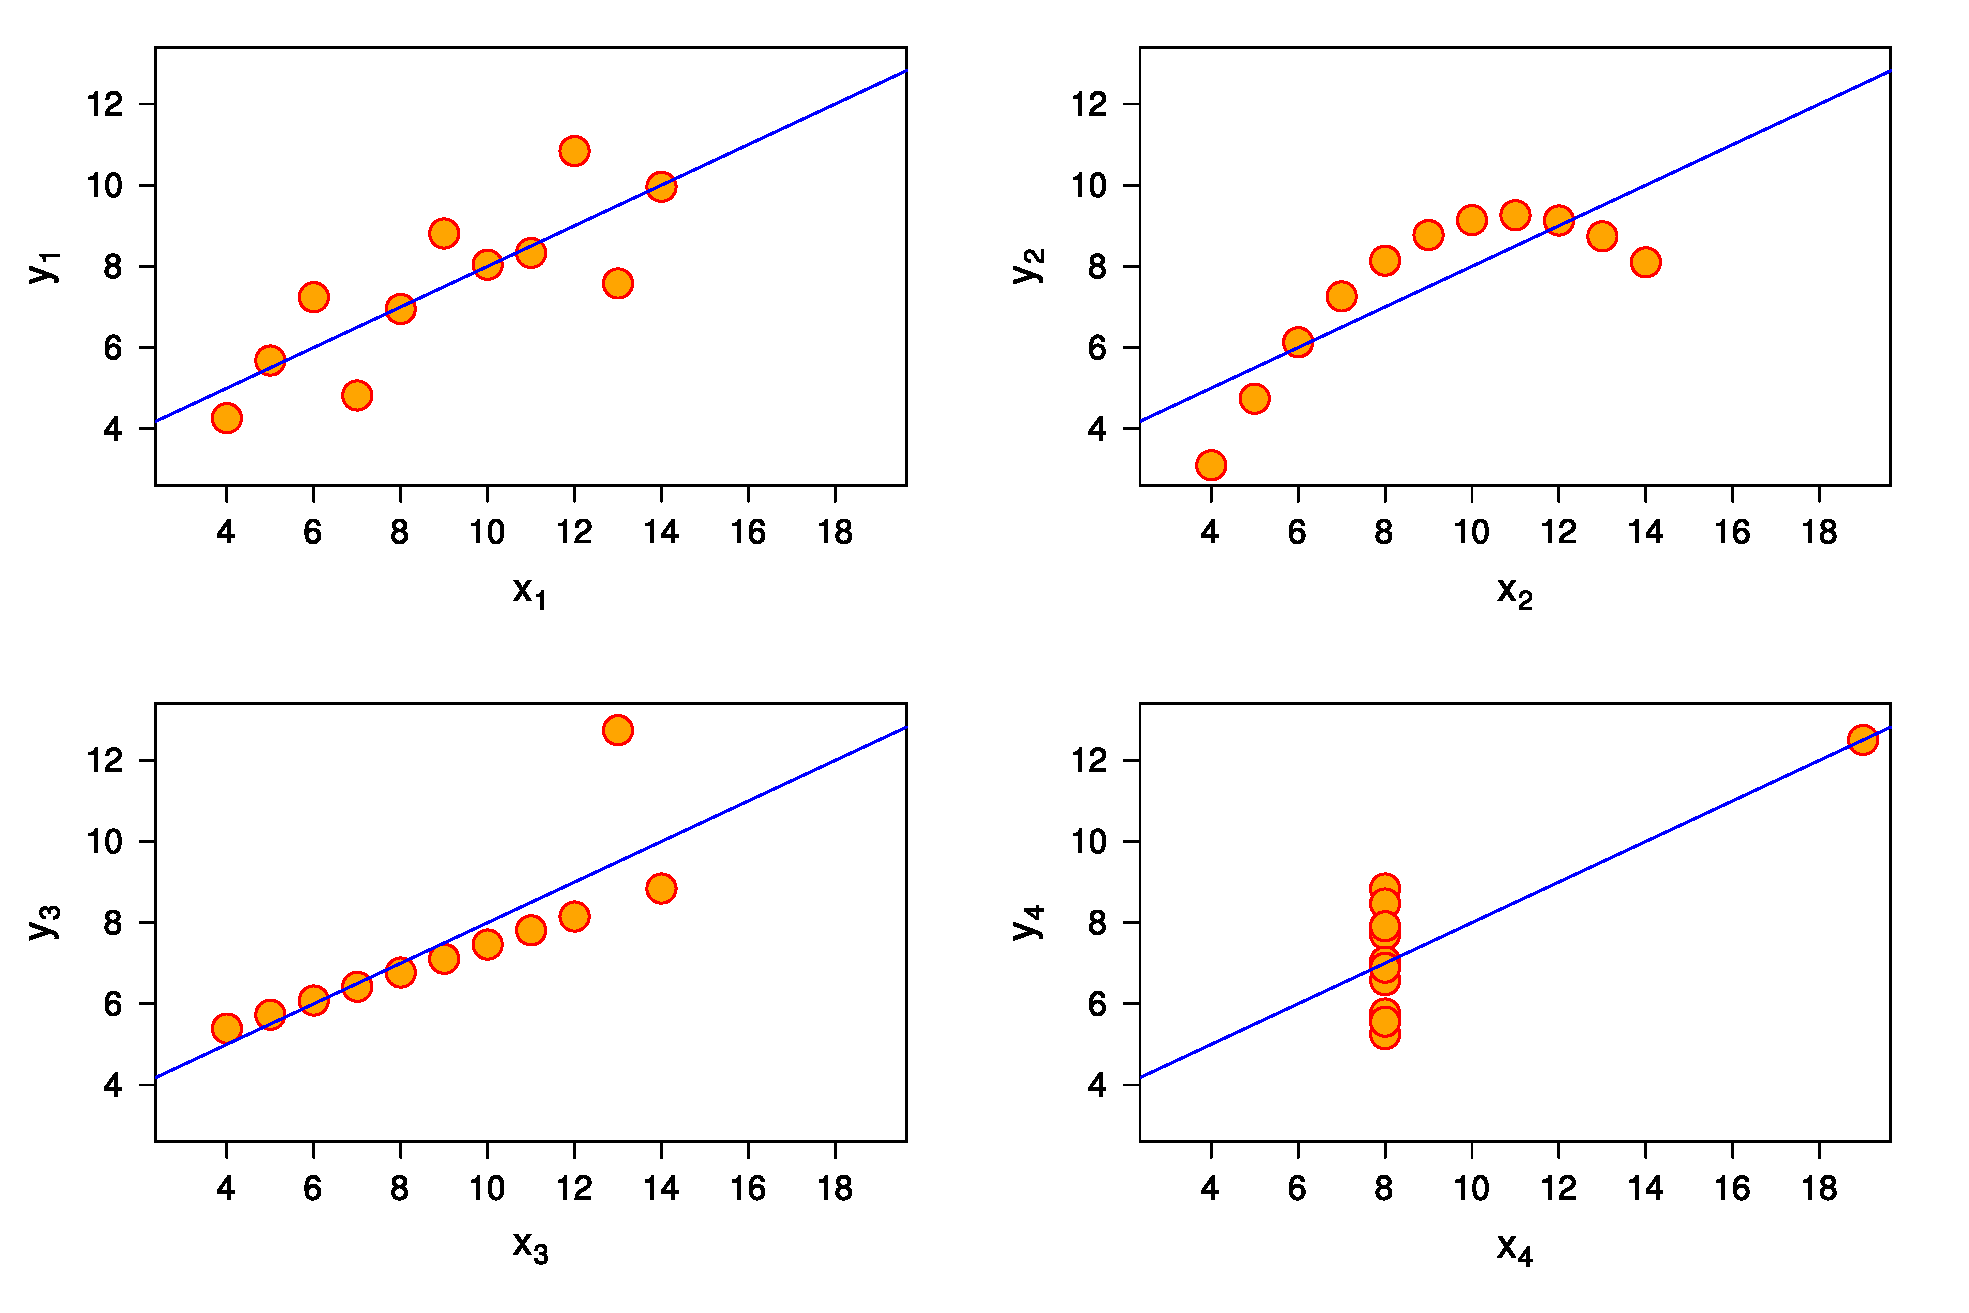
\includegraphics[width=0.8\textwidth]{static/figures/RelatedWork/Anscombe.pdf}
    \caption{Anscombe quartet. The four datasets have the same descriptive statistics (average, variance, correlation coefficient) but very different structures. Image from \cite{anscombeGraphsStatisticalAnalysis1973}.}
    \label{fig:anscombe-quartet}
\end{figure}

A large number of visualization techniques emerged to make sense of the diversity of data produced, such as multidimensional, temporal, spatial, or network data \cite{shneidermanEyesHaveIt1996}.
Instead of using taxonomies classifying graphics into categories such as histograms, pie charts, and stream graphs, some theorized how to describe graphics in a more systematic and structural way.
In 1993, Wilkinson extended Bertin's work and developed the Grammar of Graphics \cite{wilkinsonGrammarGraphics1993} as a way to describe the deep structure unifying every possible graphics, thus allowing to characterize and create graphics using common terms and rules.
In this framework, a graphic can be defined as a function of six components: data (a set of data points and attributes from a dataset), transformations (statistical operations which modify the original data, \eg mean and rank transformations), scales (\eg linear and log scales), coordinate systems (\eg cartesian and polar coordinate systems), elements (graphical marks such as rectangular or circular marks, and their aesthetics, \eg color and size), and guides (additional information such as axes and legend).
Many well-known visualization toolkits are now based on this framework, such as vega and ggplot, as it allows great expressiveness and reusability for graphic creation.
Visualization allows to gain insight on the structure of a given data, and has traditionally been used for confirmation and communication purposes, for example to verify hypothesis on empirical sciences, and later on to communicate findings.
%Many scientists use graphics to confirm hypothesis they have on their data, and later on to communicate their findings.
Visualization is also used to communicate information to wider general audiences, for example in the context of data journalism to support a point.


%Subfields of Visualization emerged: \textbf{Scientific visualization} focus on visualizing continuous real data such as weather, spatial, and physics data, sometimes produced with simulations whereas \textbf{Information Visualization} is centered around the visualization of (multidimensional) discrete data points, often in an abstract way. \textbf{Visual Analytics} emerged later from Information Visualization by mixing data mining and more complex analysis process with traditional information visualization displays.
%Historical Social Network visualization is closely related to Information Visualization and Visual Analytics, and good visualization systems for HNR use concepts and methodologies from those two fields.


\subsection{Visual Analytics}

Visualization can also be used for exploratory aims, to gain new insights on the general structure of the data and potentially generate new hypotheses.
This process has been characterized by Tukey in 1960 as \emph{Exploratory Data Analysis} \cite{tukeyExploratoryDataAnalysis1977} and consist in trying to characterize the structure of a dataset with the help of visualization and statistical measurements.
Visual exploration is enhanced by direct manipulation interfaces through interaction and usually follows the information-seeking mantra formalized by Schneiderman: ``Overview first, zoom and filter, then details-on-demand"" \cite{shneidermanEyesHaveIt1996}.
It allows users to first have a visual overview of the data and get an idea of its overall structure, to then change the point of focus to highlight interesting patterns with the help of filtering, querying, sorting, and zooming mechanisms.
%Exploration is enhanced by direct manipulation interfaces and interaction, which allows changing the point of focus in the data to highlight interesting patterns, with the help of filtering, querying, sorting, and zooming mechanisms.
%Most visual exploration interfaces are based on Schneiderman information-seeking mantra: ``Overview first, zoom and filter, then details-on-demand"" \cite{shneidermanEyesHaveIt1996}.
As the average size of datasets keeps growing, exploratory tools are often needed to make sense of large datasets and generate interesting hypotheses.

%Moreover, with the develpment of data mining and machine learning methods,
%Social scientists also often want to gain insight with the help of statistical and machine learning methods, that visualization only can not provide.
More recent visual exploration interfaces also incorporate automatic analytical tools along with graphical displays, letting users apply data mining algorithms directly in the exploratory loop.
This coupling of visualization and data mining has been defined as Visual Analytics (VA) and is still undergoing lots of research.
Keim and al.\ define it as ``a combination of automatic and visual analysis methods with a tight coupling through human interaction in order to gain knowledge from data'' \cite{keimVisualAnalyticsDefinition2008}. \autoref{fig:keim-va} shows an abstract representation of the VA process.

%\begin{figure}
%    \centering % avoid the use of \begin{center}...\end{center} and use \centering instead (more compact)
%    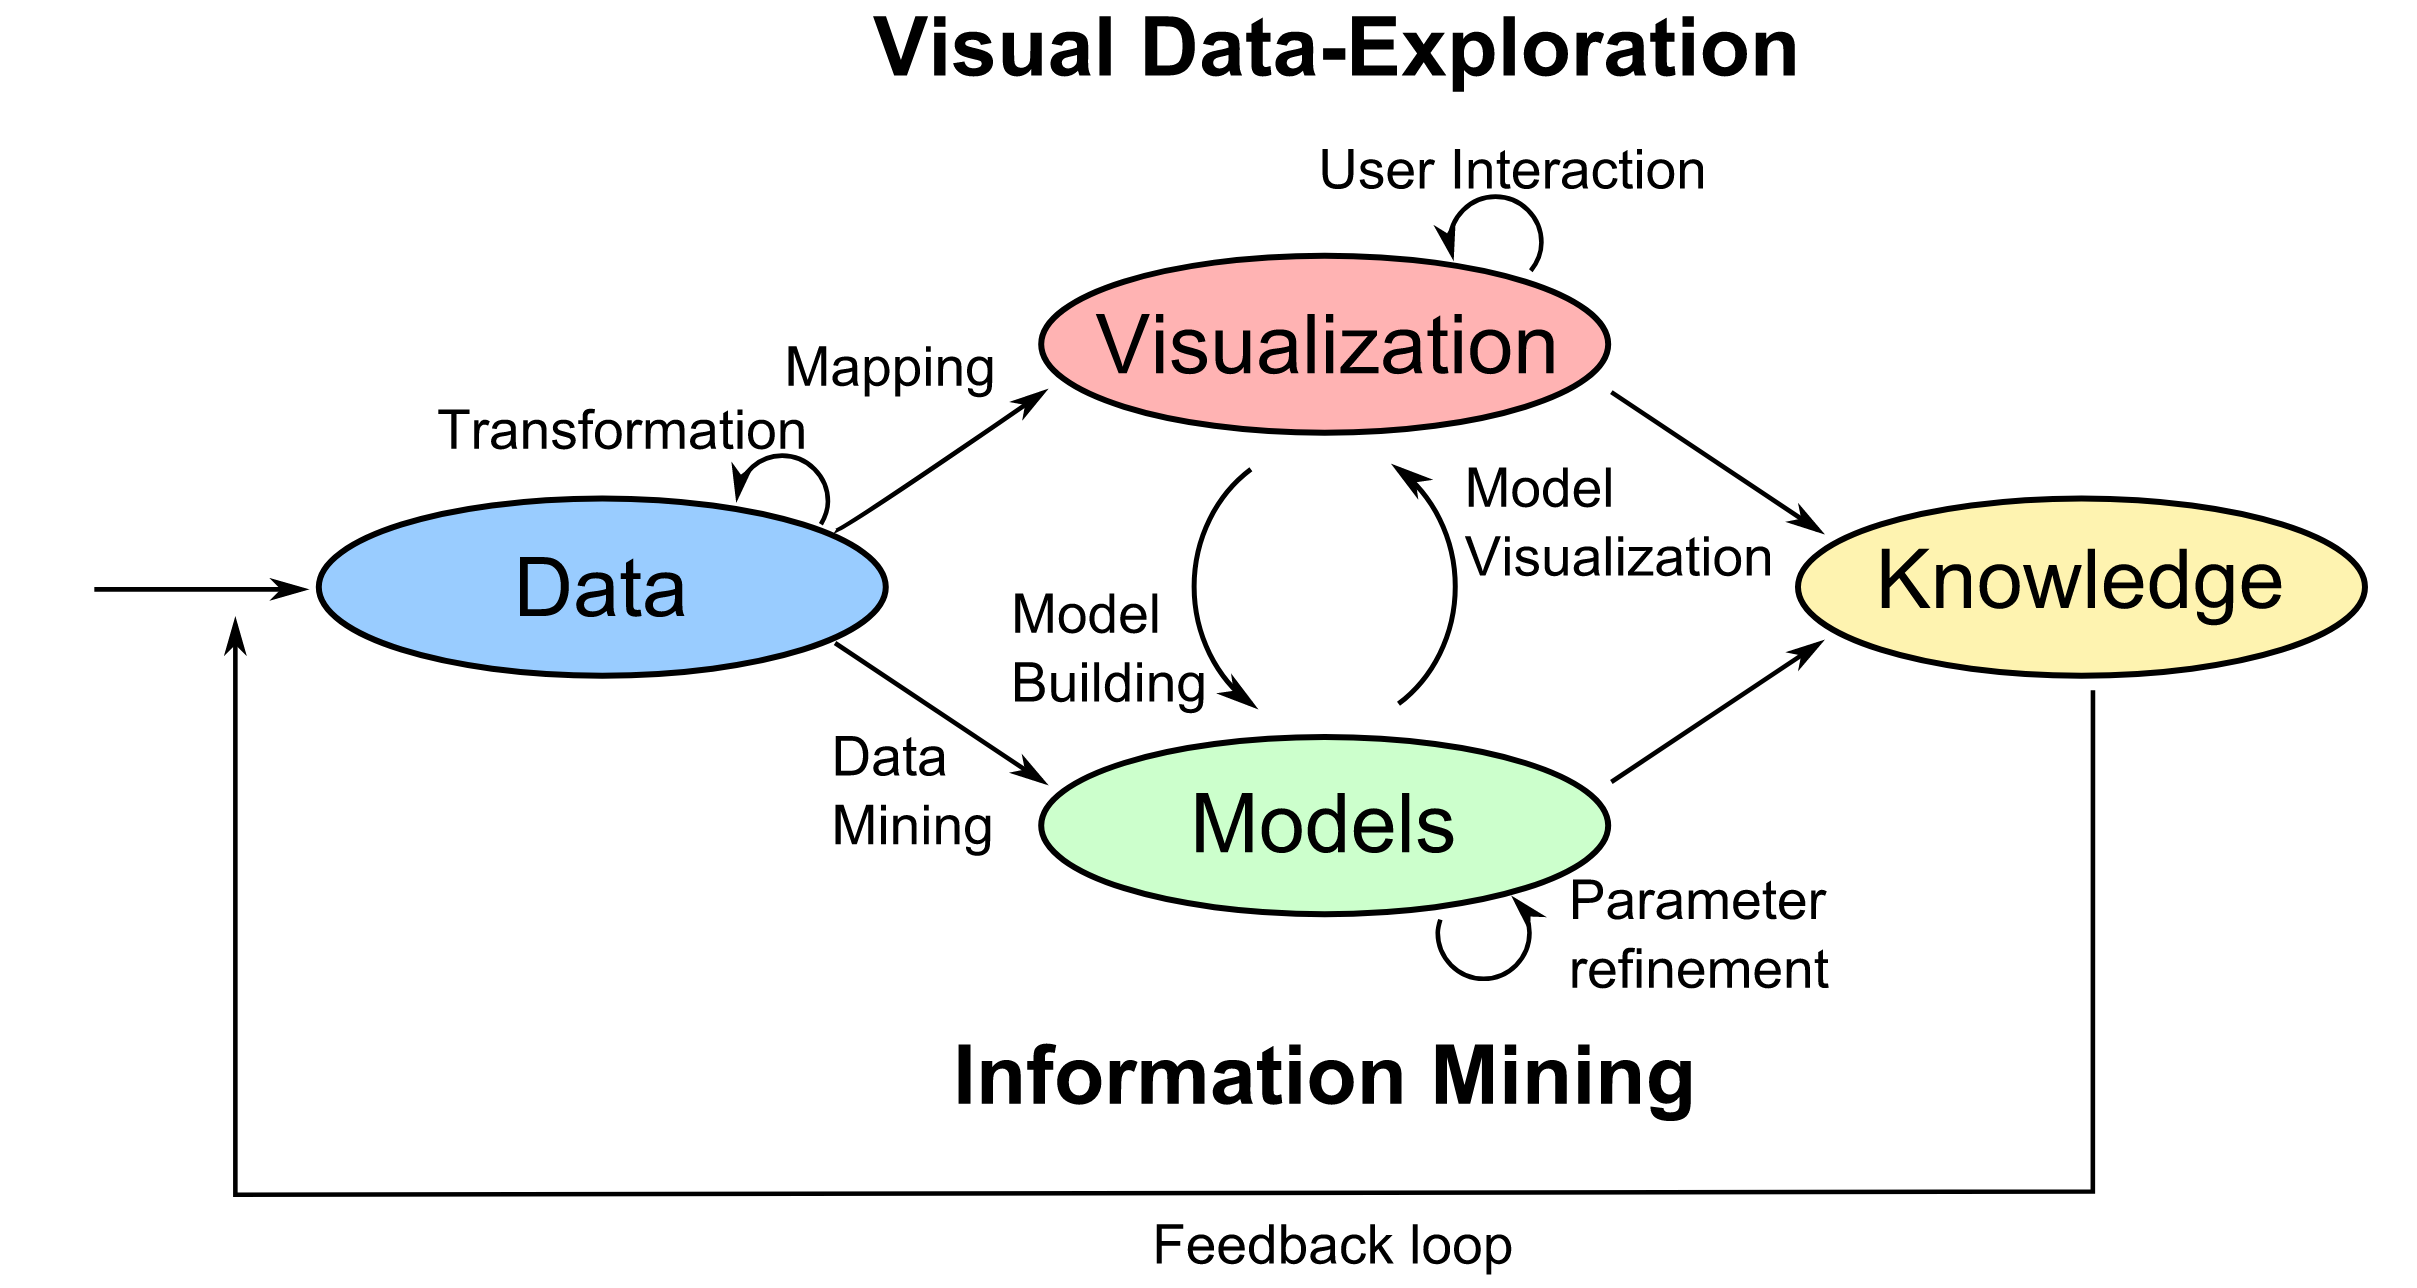
\includegraphics[width=1\textwidth]{static/figures/RelatedWork/Keim-VisualAnalytics.png}
%    \caption{Abstraction of the VA process. It is characterized by continuous interactions between the data, visualizations, models, and knowledge. Image from \cite{keimVisualAnalyticsDefinition2008}.}
%    \label{fig:keim-va}
%\end{figure}

It is defined around the generation of knowledge using visualizations and models of the data, that the user generates and explores using interaction.
VA systems have been developed in various empirical domains, such as biology, astronomy, engineering, and social sciences, as it allow to rapidly gain insight on the structure of various potentially large dataset, while generating and refuting hypotheses. %but are nonetheless not used by the majority of application scientists.
%Indeed, there are currently debates on the roles of EDA and VA in the scientific process, as exploratory findings do not have the same level of proof than statistical results coming from the hypothetico-deductive model.
%\eda and \va are nevertheless efficient tools to refute and generate hypothesis, especially with the ever-increasing amount of stored data.


%Social scientists now frequently use VA systems to make sense of their data by using visualization, interaction, and data mining algorithms in their analysis loop to find interesting patterns and verify and create hypotheses.
%The most used social network VA tools are Gephi \cite{Gephi}, Pajek \cite{mrvarAnalysisVisualizationLarge2016}, and NodeXl \cite{NodeXL}. \autoref{fig:gephi} presents the Gephi interface showing a clustered social network, where each node is part of a cluster, encoded by color.
%They all let users visualize their networks with a node-link diagram, and allow an interactive exploration of the data with operations like filtering.
%Users can also analyze their data using network measures computed directly in the interface, and apply data mining algorithms such as clustering which results are explorable visually.



\section{Social History}\label{sec:historical-network-research}

If Sociology and Anthropology started to use network concepts and methods rapidly in the 1950s, it was not until the 1980s that historians started to use this type of methodology.
Yet, historians started to use quantitative methods in the 1960s, with the rise of social history, by extracting information from historical textual documents and studying them with statistical methods.
When seeing the potential of SNA concepts for historical purposes, historians started to extract the relational information contained in documents to study historical social phenomena using the power of networks and methods already developed in SNA.


\subsection{History, Social History and Methodology}\label{subsec:history-and-social-history}

The concept of History is hard to define as its practice and cutomes highly evolved through time \cite{prost2014}.
History of a given time can be characterized by the different historical work produces at that time.
However, the work of the historians always focused on the collection and study of historical documents, to characterize the past.
As Langlois and Seignobos write, ``The search for and the collection of documents is thus a part, logically the first and most important part, of the historian's craft'' \cite{langloisIntroductionAuxÉtudes2014}.
History emerged as a field with its own rules, conventions and journals in the 1880s from faculties of letters, to counterbalance previous history works which were judged as too ``literary'' \cite{noirielNaissanceMétierHistorien1990}.
History can be seen through two facets: one is societal, and serves creating a shared story for the country and a sense of unity to its citizens.
Antoine Prost says that ``it's through history than France thinks itself'' (translated from french) \cite{prost2014}.
The second facet of history constitute a methodology to describe the past in a rigorous and scientific way, with proofs.
For this, historians rely on historical documents that they leverage to infer dated facts about the past (the temporal aspects of conclusions is always central to the historian work).
The textual sources are thus at the core of the work of the historians, and having to cite historical documents and previous peers work to new claims is primordial to be considered as rigorous History work.
However, even if those two aspects are well characterized (temporal aspect of the work and its relationships to sources), methodological and epistemological facets (how historians should read and analyze their sources, how to cite them, what to report/not report etc.) of History have not been studied and discussed for a long time, until the end of the 1980s.
Some historians were interested in historiography \cite{carbonellHistoriographie1981}, but none were going to philosophical and epistemological reflexions of the History discipline.
For Lucien fèbvre, philosophising was even constituting a ``capital crime'' \cite{febvreVERSAUTREHISTOIRE1949, prost2014}.
%Les historiens font ordinairement de l’histoire sans méditer sur les limites et les conditions de l’histoire  ; sans doute, ils ont raison ; il vaut mieux que chacun fasse son métier ; d’une façon générale, il vaut mieux qu’un historien commence par faire de l’histoire sans en chercher aussi long : autrement, il n’y aurait jamais rien de fait

%\alexis{maybe talk about the positivists and methodists}
At the start, history was mainly event-centered, and was focusing in characterizing central figures of the past like rulers and artists or shed light on events which shaped history like wars or political crisis.
This narrative approach to history has been criticized for its open interpretation of historical documents, which can introduce bias from the authors \cite{bourdieuRapportsEntreSociologie1995}.
%Social History emerged as a sub discipline of history with a focus on the social ascpect of history, trying to link political events (such as a revolution) to

In the 1930s, March Bloch and Lucien fèbvre detached from traditional history by creating the ``Annales school'' (Ecole des Annales) which tried to replace the human as a component of a broader sociological, political and economic system with influences between each other \cite{burkeHistorySocialTheory2005}.
They strongly advised to exhaustively search from archives, to ground historical results in documents, texts and numbers.
This new way of studying past events and societies became successful in a profession in crisis, by bringing a new lens of study on various societal subjects more grounded in the real and with a better intelligibility.
This school of thought can be seen as one of the biggest milestones for Social History, a branch of History which focuses on the socio-economical aspects of societies and their changes through time, rather than an event-centric view of History.
For example, in his thesis, Ernest Labrousse---a well known figure of Social History---tries to describe and explain the economic crisis of France at the end of the ``Ancien Régime''\footnote{The ``Ancien Régime'' is an historical period of France which starts from the beginning of the reign of the Bourbon house at 1589 until the Revolution in 1789.} through the evolution of the economic power of different social groups such as farmers, workers, property owners etc\. instead of solely describing memorable facts about the period \cite{labrousse1990crise}.
Social History continued to evolve since the 1930s, introducing new methods and concepts, but always with the goals to describe periods and historical facts through a sociological lens and with a strong focus on sources and traceability.



\subsection{Quantitative History}\label{subsec:quantitative-history}

\todo{Cliometrics}

%Historians try to understand an epoch using textual sources from the past, and trying to extract useful information from them.
%Social history, which is a branch of history, focus on understanding how societies were organised and how people were living together at a particular time and place. Charles Tilly argued that the task of social history lays in "(i) documenting large structural changes, (2) reconstructing the experiences of ordinary people in the course of those changes, and (3) connecting the two". For the latter, historians can leverage personal written sources---such as letters, journals, books, and newspapers---to have the internal point of view of persons living in this society and descriptions of lives of precise individuals.
%For the former, historians usually need to study more structured documents which contain information which can be extracted in a predefined and exhaustive way.
%These documents can for example be census, migration acts or marriage acts. By studying theses documents and by systematically extracting the information of these documents, historians can make global and quantitative conclusions on certain social and behavioural aspects of societies of interest.
%For example .. [EXAMPLE CHANGEMENT METIERS XXth century]

%Traditionally, historians try to tell a story about protagonists and socio-economic facts in a given society by reading, understanding, and linking together historical sources.
%This narrative approach to history has been criticized for its lack of traceability and the open interpretation of historical documents, which can introduce bias from the authors.
%To solve this problem, the ``Annales school'' (Ecole des Annales) proposed to characterize past social phenomena through the exhaustive and systematic analysis of historical documents~\cite{prost2014}.

With the development of statistical methods and Computer Science, quantitative approaches of History emerged in the 1960s with the aim of analyzing quantitative data directly extracted from historical documents.
%Using quantitative data, historians were able to make numeric conclusions on topics such as demography \cite{henryRegistresParoissiauxHistoire1956} or job distribution.
Using such methods, historians were able to make conclusions based on statistical results on topics such as demography \cite{henryRegistresParoissiauxHistoire1956} or job distribution.
For example, Gribaudi and Blum illustrated a shift in the most widespread professions in France during the 19th century using the data extracted from 50000 marriage acts \cite{gribaudi1990} and using statistical methods.

Unfortunately, quantitative and numerical methods have been criticized by historians for their simplifications and for consuming considerable time while often providing simple results \cite{karila-cohenNouvellesCuisinesHistoire2018,lepetitHistoireQuantitativeDeux1989}.
Trying to understand complex historical phenomena is complicated and modeling the information contained in historical documents into quantitative datasets can rapidly simplify and distort reality.
Moreover, quantitative historians have been criticized for focusing too much on the data, neglecting the original sources which give the context in which the data has been produced \cite{lemercierQuantitativeMethodsHumanities2019}.
Guildi and Aritage went as far as criticizing the decrease of interest of historians working in archives \cite{guldiHistoryManifesto2014}.
Approaches using digital methods and tools are nonetheless more and more popular, sometimes more recently referred to under the umbrella term Digital Humanities (DH).
If their adoption remains slow and sometimes criticized among historians, they still provide tools to store, explore, and analyze historical documents systematically if used appropriately (i.e.\ not trying to bias the analysis, and not losing the trace of the original sources).
DH can also provide infrastructures and tools to study large historical databases which is more complicated to do by hand, as with the Venice Time Machine project~\cite{kaplanVeniceTimeMachine2015} which aims at digitizing and analyzing thousands of documents from the archives of Venice to understand the political, geographical, and sociological dynamics of the cities across generations and centuries.



\subsection{Digital Humanities}\label{subsec:DH}

Digital Humanities is sometimes described as the third wave of computational social sciences \cite{lemercierQuantitativeMethodsHumanities2019}.
The term have gained popularity since the 2010s and refer to ``research and teaching taking place at the intersection of digital technologies and humanities. DH aims to
produce and use applications and models that make possible new kinds of teaching and research, both in the humanities and
in computer science (and its allied technologies). DH also studies the impact of these techniques on cultural heritage,
memory institutions, libraries, archives and digital culture.'' \cite{terras2011quantifying}.
If the first waves of computational social sciences focused a lot on mathematical computations such as hypothesis testing and correlation computations to make conclusions, DH focuses also on the teaching, communication and exploration of humanities datasets and concepts, through the help of design, infographics and interactive systems \cite{burdickDigitalHumanities2016}.
In the context of historical research, the term Digital History have been coined as ``an approach to examining and representing the past that works with the new communication technologies of the computer, the Internet network, and software systems. On one level, digital history is an open arena of scholarly production and communication, encompassing the development of new course materials and scholarly data collections. On another, it is a methodological approach framed by the hypertextual power of these technologies to make, define, query, and annotate associations in the human record of the past. To do digital history, then, is to create a framework, an ontology, through the technology for people to experience, read, and follow an argument about a historical problem.'' \cite{InterchangePromiseDigital2008}
%Digital History therefore focus a lot on the curation and exploration of historical archives in the purpose of characterizing and communicate of historical concepts.
Digital History therefore focus a lot on the curation and digitization of historical archives, the identification of historical concepts through computational and exploration methods, but also their communication to the general audience through digital technologies.

\begin{figure}
    \centering % avoid the use of \begin{center}...\end{center} and use \centering instead (more compact)
    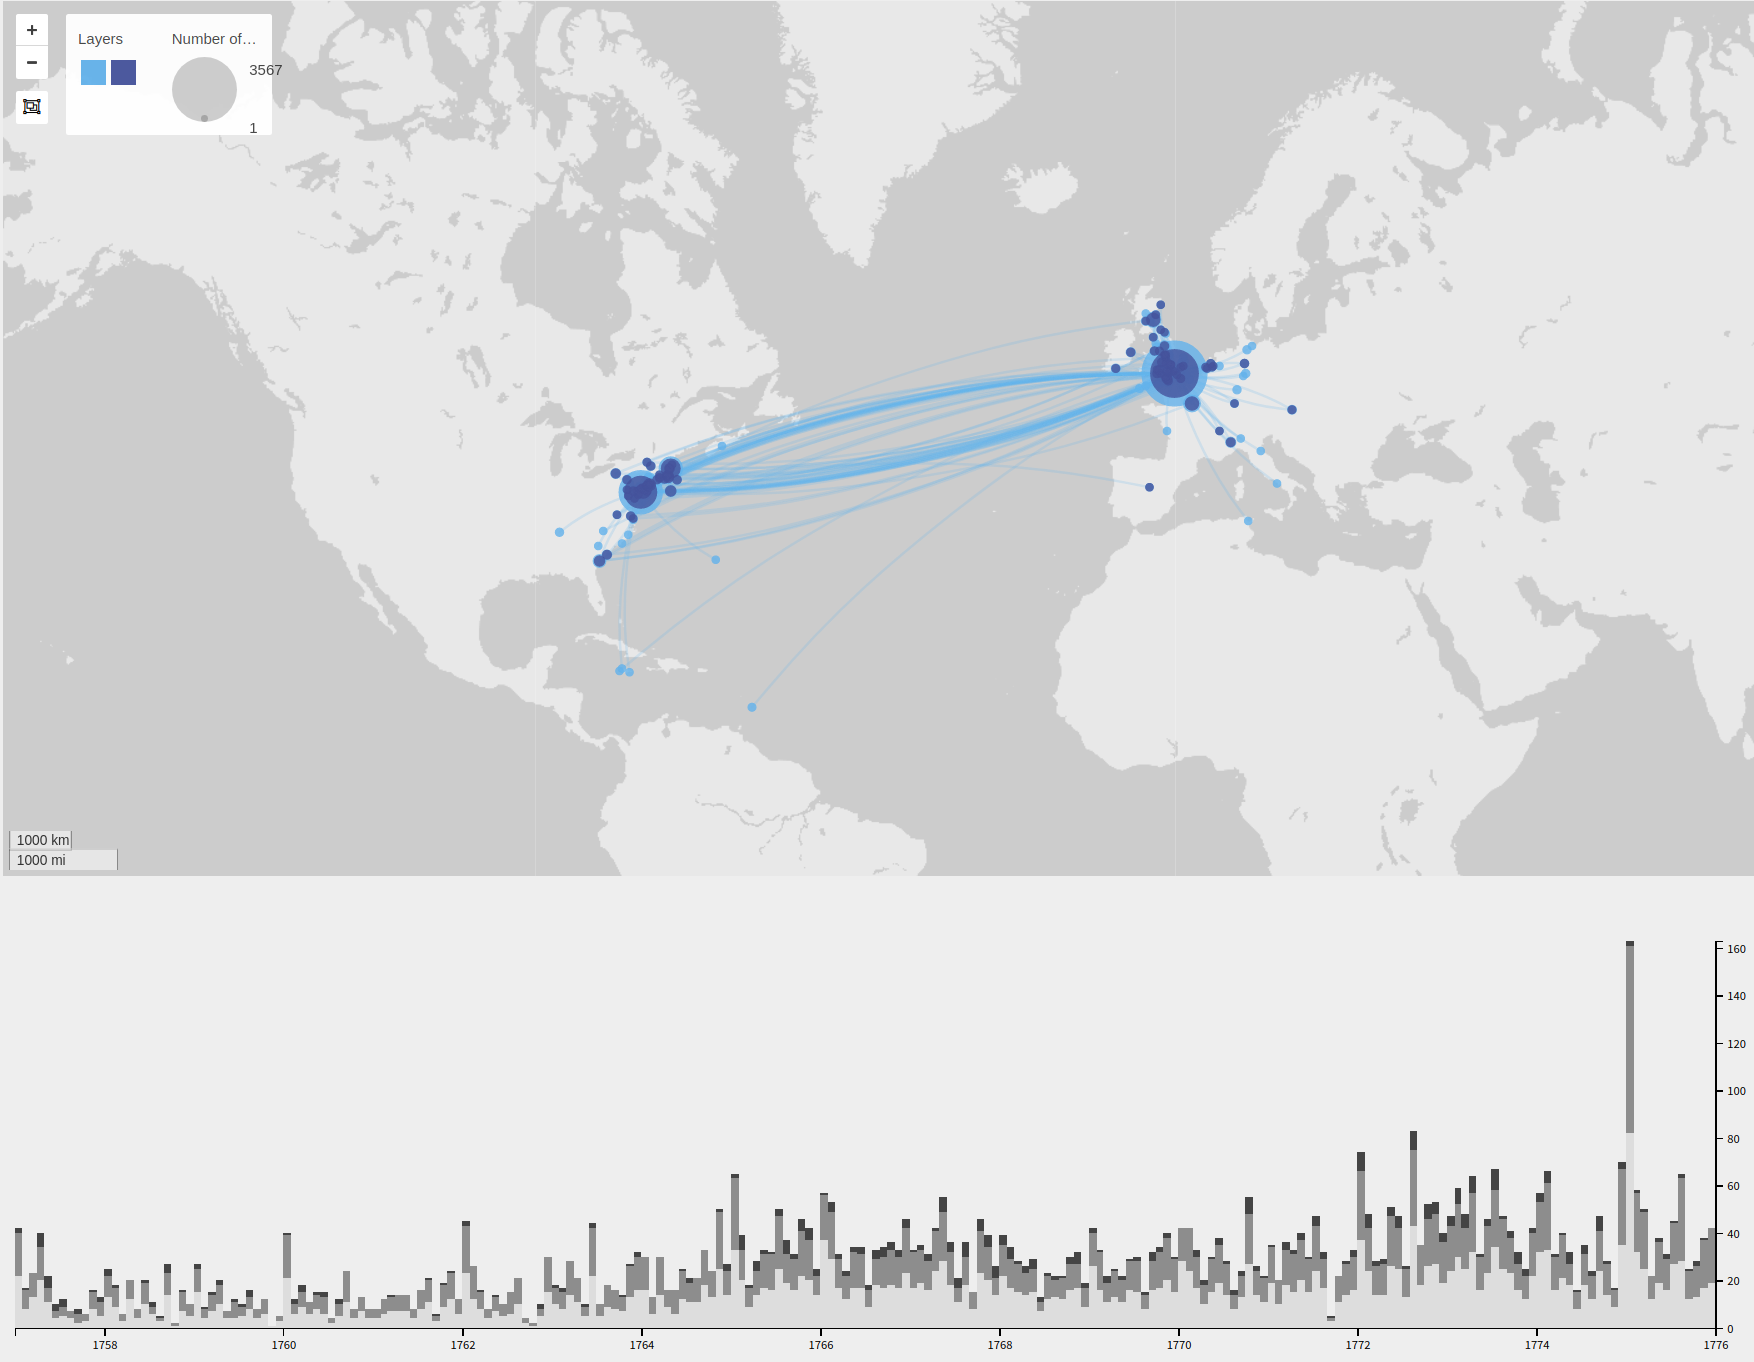
\includegraphics[width=1\textwidth]{static/figures/RelatedWork/RepublicOfLetter_BenjFranklin}
    \caption{Correspondence letters of Benjamin Franklin and his close relationships, using a map and an histogram, accessible online on the republic of letter website.}
    \label{fig:republic-letters}
\end{figure}

A lot of Digital History projects are thus multidisciplinary by essence and involve several teams of researchers, such as the Republic of Letters project which consisted in digitizing, storing and exploring letters of scholars across the world, in a common hub and using shared visualization tools \cite{edelsteinHistoricalResearchDigital2017}.
It resulted in the elaboration of curated datasets and visualizations concerning the correspondence of various scholars such as Voltaire, Benjamin Franklin (see \autoref{fig:republic-letters}), or John Locke, accessible in the same place by researchers and the general audience.

With modern technologies and infrastructures, it also becomes possible to study large historical databases as with the Venice Time Machine project~\cite{kaplanVeniceTimeMachine2015} which aims at digitizing and analyzing thousands of documents from the archives of Venice to understand the political, geographical, and sociological dynamics of the cities across generations and centuries.
A lot of projects which claim themselves as Digital History also leverage network methods and concepts \cite{ahnertNetworkTurnChanging2020}, such
as the Viral Texts \cite{cordell2017viral} and Living with Machines \cite{ardanuyLivingMachinesStudy2020} projects which respectively study nineteenth-century newspapers and the industrial revolution by translating their sources into analyzable networks.
We discuss more in depth the related work of network analysis for historical research in \autoref{subsec:hsna}.


\section{Historical Social Network Analysis}\label{sec:hsna}


SNA is defined as an ``approach grounded in the intuitive notion that the patterning of social ties in which actors are embedded has important consequences for those actors. Network analysts, then, seek to uncover various kinds of patterns. And they try to determine the conditions under which those patterns arise and to discover their consequences'' \cite{freeman_development_2004}.
The concept of SNA emerged in sociology in response to traditional methods using pre-defined taxonomies and social categories to understand and explain sociological behaviors and phenomena, which could introduce bias.
By modeling real observed social relationships and interactions with networks and by using mathematical and statistical methods to study those, sociologists have been able to explain sociological phenomena and describe sociological interactions through their direct observation modeled as networks.
%SNA is now a well-praised methodology in sociology, which has also been extended to History to study relational aspects of societies and institutions of the past.
SNA is now a well-praised methodology in sociology and has been extended to historical research to study relational concepts such as kinship, friendships, and institutions of the past.
Social historians leverage their documents to extract relationships between entities---often persons---that they model into networks.
Using network concepts and visualization tools, they can make conclusions through structural observations of such networks.


%which has also been extended to History to study relational aspects of societies and institutions of the past.


\subsection{Sociometry to SNA}

One of Sociology's main goals is to study social relationships between individuals and find recurrent patterns and structures allowing to explain the behaviors of people and groups.
Traditional methods try to explain social phenomena using classical social classifications such as age, social status, profession, and gender.
For example, the socio-economic position of people living in a small city could be explained by their age, demographics, and family status which are traditional social categories.
However, some criticism emerged that this type of division is often partially biased and comes from predefined categories which are not always grounded in reality.
Sociometry is considered one of the bases of SNA and had the goal of redefining social categories through the lens of real social interactions and ties between persons, that sociologists wanted to observe in real conditions.
It is in the 1930s that Moreno started to develop this new method by trying to depict real social interactions as a way to understand how groups and organizations were functioning \cite{morenoFoundationsSociometryIntroduction1941}.
He developed sociograms as a way to visually show friendships between people with the help of circles representing persons and lines modeling friendships.
\autoref{fig:moreno-sociogram} shows one of Moreno's original sociograms to depict friendships in a class of first grades (left).
%This way, he could rapidly see the main actors and hubs of interaction inside the social network represented visually.
Sociometry tremendously helped disseminate the metaphor of networks to model and understand social structures and phenomena.
It was during the 1960s that sociologists and anthropologists took these concepts further and formalized SNA using graphs and mathematical methods, following the emergence of Graph Theory studies in the 1950s by Mathematicians such as Erd\H{o}s \cite{erdos2011}.
%It did not take long until sociologists used these concepts to model social ties and relationships into graphs.
Sociologists already had structural theories of social phenomena, and they rapidly saw the potential of networks\footnote{Graphs and networks refer to the same thing but are often used in different contexts. The term graph is preferred in a mathematical and abstraction setting, while the term network is mostly used when modeling real-world phenomena. We talk about nodes and links for networks and vertices and edges for graphs.} to model social relationships between actors, representing the persons as nodes and relationships as links.
Graph theory brought a panoply of concepts and methods to study and describe networks, that sociologists such as Coleman started to codify to use in a sociology setting \cite{colemanIntroductionMathematicalSociology1964}.
Using mathematical and network methods, it was possible to formally describe social relationships to make sociological conclusions grounded in real observations modeled as networks.


\begin{figure}
    \centering % avoid the use of \begin{center}...\end{center} and use \centering instead (more compact)
    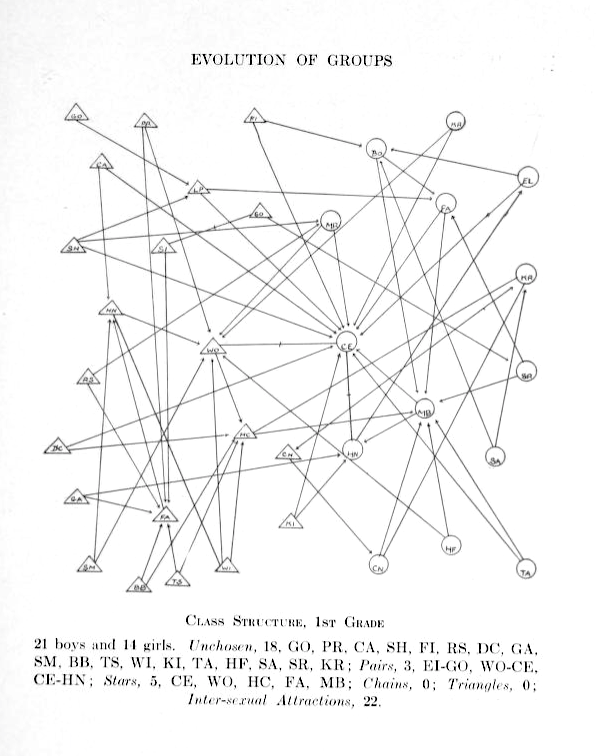
\includegraphics[width=0.4\textwidth]{static/figures/RelatedWork/Moreno-1}
    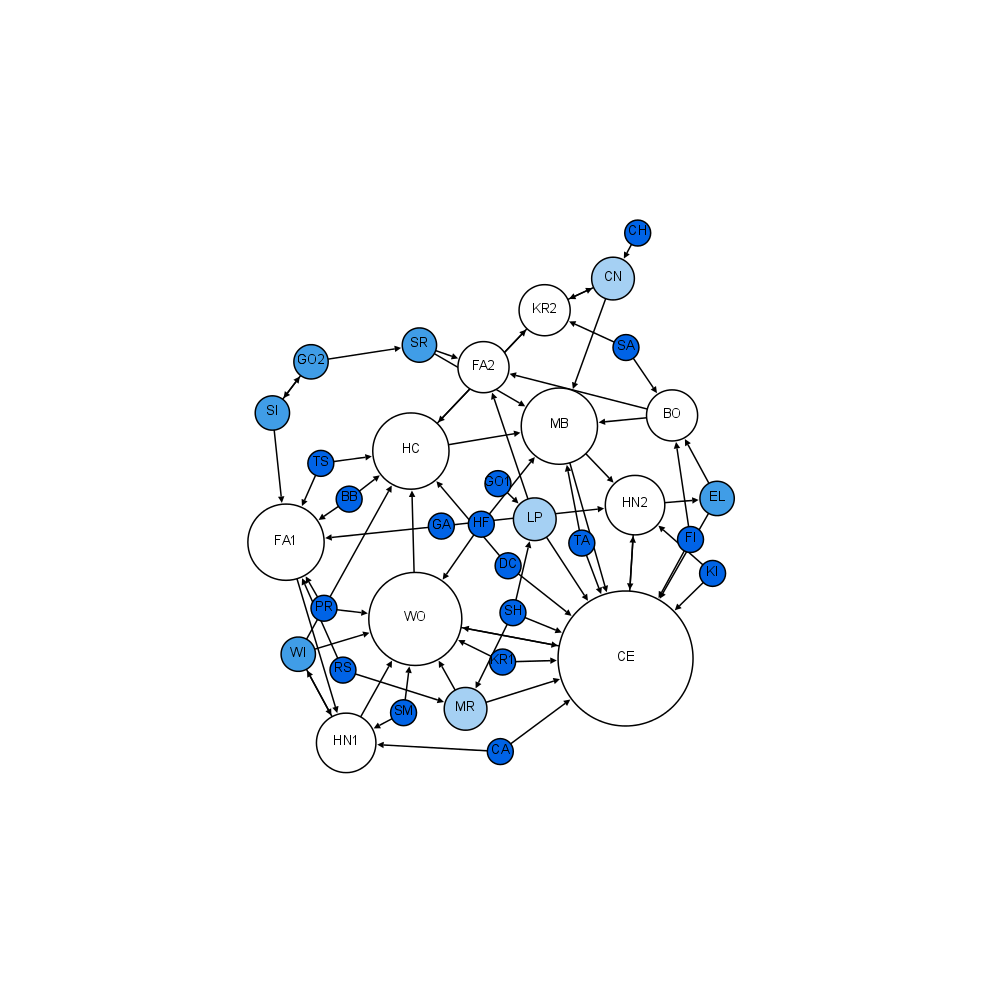
\includegraphics[width=0.55\textwidth]{static/figures/RelatedWork/Moreno-1_GrandJean}
    \caption{Moreno's original sociogram of a class of first grades from \cite{morenoWhoShallSurvive1934} (left). The diagram shows 21 boys (triangles) and 14 girls (circles). The same sociogram plot using modern practices generated from Gephi from \cite{grandjeanSocialNetworkAnalysis2015}. The color encodes the number of connections incoming.}
    \label{fig:moreno-sociogram}
\end{figure}



\subsection{Methods and Measures}

%After SNA started to be formalized, lots of sociological studies used those concepts.
%Many sociological studies used SNA concepts after it has been formalized.
%However, there were not yet strong protocols and methods to follow, and networks are an abstraction that can model different things in different ways.
%When looking retrospectively, we can see that two schools of thought emerged with different objectives and methods: the structuralists and the school of Manchester \cite{eveDeuxTraditionsAnalyse2002, maurizio2000, freemanDevelopmentSocialNetwork2004}.

The goal of SNA is to study the structure of a given network to make sociological conclusions.
Yet, two distinct methodologies emerged through the history of SNA: the structuralists and the school of Manchester \cite{eveDeuxTraditionsAnalyse2002, maurizio2000, freemanDevelopmentSocialNetwork2004}.


%The Structural Analysis of Social Network refer to the Structuralists in Sociology.
The structuralists are interested in observing the relational structures and patterns forming a network, to make parallels between them and the social behaviors of actors in real life \cite{lazegaReseaux}.
They think the positions of the persons in the network and the relational patterns they are part of reflect well the social activities and behavior in real life.
Studying those would thus allow them to make interesting sociological conclusions.
Accordingly, sociologists in this school usually study organizations and specific groups---such as institutions, companies, families, etc.---and want to explain their functioning through the description of the internal shapes and structures of the networks.
Thus, they try to construct networks that exhaustively model all the interactions between the actors constituting the groups, as missing links would misrepresent the reality of interactions.

In contrast, the school of Manchester constituted by anthropologists focuses on studying specific individuals and all their interactions in the different facets of their lives and through time.
They typically want to explain certain behaviors and social characteristics of individuals by their relationships and interactions in all their complexity and highlight the influence of different social aspects between them in one's life.
One famous example is Mayer's study on austral Africa rural migrants going to cities \cite{mayerMigrancyStudyAfricans1962} where he showed that the integration of urban mores and customs were directly correlated to the persons' relationships networks in the city.
Xhosa\footnote{Xhosa people are an ethnic group living in South Africa and talking the Xhosa language. and studied} people still interacting with rural people of their village in the city were less changing their customs.
This school of thought typically relies on the concept of ego network and more recently dynamic and multiplex networks.
Ego networks are networks modeling all the direct relations of one central node---in this case, a person---including the relations existing between the persons of this small network.
They typically try to model the different types of relationships of a person, like their family, work, and friendship ties, and study them through time.
By studying the ego network structure of someone, sociologists of this school try to leverage explanations on other social aspects of the persons like their social status, job, and gender.
It is also common to compare several ego networks to make correlations between the social relationships of individuals and other interesting social categories.

%These two methodologies of SNA are often not exclusives and current studies usually involve concepts and methods from both.
These two methodologies of SNA are often not exclusives and current studies are typically inspired by those two traditions.
This is especially true in history where even if historians may want to describe exhaustively a group or institution of the past, they are almost always interested in specific individuals they study in depth.

Furthermore, the two approaches leverage similar network measures and concepts.
%Graph theoreticians and network scientists developed a myriad of graph measures (\eg density, centrality, and diameter) and algorithms that social scientists appropriated to describe and characterize social phenomena.
A myriad of graph measures (\eg density, centrality, and diameter) and algorithms have been proposed by graph theoreticians and network scientists that social scientists appropriated to describe and characterize social phenomena.

When constructing networks, the first thing sociologists do is to identify the main actors of the network and explain why these actors are the most central, for example by linking it to their profession or social status.
Computing the degree---which is the number of connections for a node---distribution is the main straightforward way of doing it, but other more complex measures like centrality have also been developed.
Several types of centrality measures (\eg betweenness, closeness) have been proposed, based on different criteria, as there are several ways of defining the more important actors.
Some centrality measures highlight actors with the highest number of connections while others highlight people bridging different groups with low interactions.
More generally sociologists aim at identifying recurring patterns of sociability between actors.
The concepts of dyads and triads counting, which are basic structural patterns of 2 and 3 nodes, give insights into low-level relationships between people.
This reflects on Simmel's formal sociology, where he already referred to dyads and triads as a primal form of sociability \cite{Simmel2013}.
More recently, graphlet analysis extended this concept to every pattern of N-entities.
Graphlet analysis aims at enumerating every small structure of $N$ nodes composing a network, to understand how people interact at a low level.
Graphlets counting shows that graphlets are not found in a uniform distribution in social networks, thus revealing that social networks usually do not have the same structure that random networks.
This is a fact well known in SNA. Precisely, entities in real-world networks tend to agglomerate into groups (also called clusters) where entities in the same groups interact more between them than with entities from other groups.
From a sociology perspective, it means that people tend to interact and socialize in groups and interact more rarely with other people from outside groups.
These groups are often referred to as \emph{communities}, and many algorithms have been proposed to find these automatically.



\subsection{Historical Social Network Analysis}\label{subsec:historical-social-network-analsyis}

History started to use concepts and methods from SNA in the 1980s~\cite{wetherellHistoricalSocialNetwork1998} in order to criticize quantitative history concepts and results,
% \cite{gribaudi_categories_1990}
and to develop historical approaches---like \textit{Microstoria} \cite{ginzburgMicrohistoire1981}---that focus on the study of individuals and groups through the lens of their interactions and relationships directly extracted from historical documents.
%History started to adopt some methods and vocabulary of Network Science in the 1980s, several years after other fields such as sociology and anthropology.
Beforehand, historians were already describing and studying relational structures such as families and organizations with qualitative methods and with classical taxonomies, without studying in depth the relational aspect of these entities.
Network research allowed them to model those relational entities more thoroughly using network concepts, thus allowing them to make new observations that it was not possible to see without taking into account the relational aspects of these entities.
%Historians already had techniques and tools to annotate and extract quantitative information from textual sources that they adapted to extract and study social ties.
%We therefore saw the emergence of HNR studies, where historians studied the social relationships of actors of the past extracted from textual document and modeled into networks.
Observing and describing the structure of the resulting networks allowed historians to make conclusions on sociological aspects of the past, similar to SNA.
%followed SNA protocols on networks constructed from the mention of social ties of their textual sources.
%Using similar concepts of SNA, describing the network of social relationships of the past,
Since then, HSNA---a term coined by C. Wetherell in 1998 \cite{wetherellHistoricalSocialNetwork1998}---has been applied by historians to study multiple kinds of relationships, like kinship and political mobilization \cite{lippKinshipNetworksLocal2005}, administrative and economic patronage \cite{moutoukias1992}, etc.
If these approaches fall under similar critics as quantitative history \cite{lemercier12FormalNetwork2015} like leading of trivial conclusions, it still led to classical work and interesting discoveries.
One famous example is the study of the rise of the Medici family in Florence in the 15th century by Padgett \cite{padgettRobustActionRise1993}, where he explained the rise of power of this family by their central position in the trading, marriage, and banking networks of the powerful families of Florence. \autoref{fig:padgett-medicis} shows the different networks of Florence families where we can see the central position of the Medici.

\begin{figure}[!ht]
    \centering % avoid the use of \begin{center}...\end{center} and use \centering instead (more compact)
    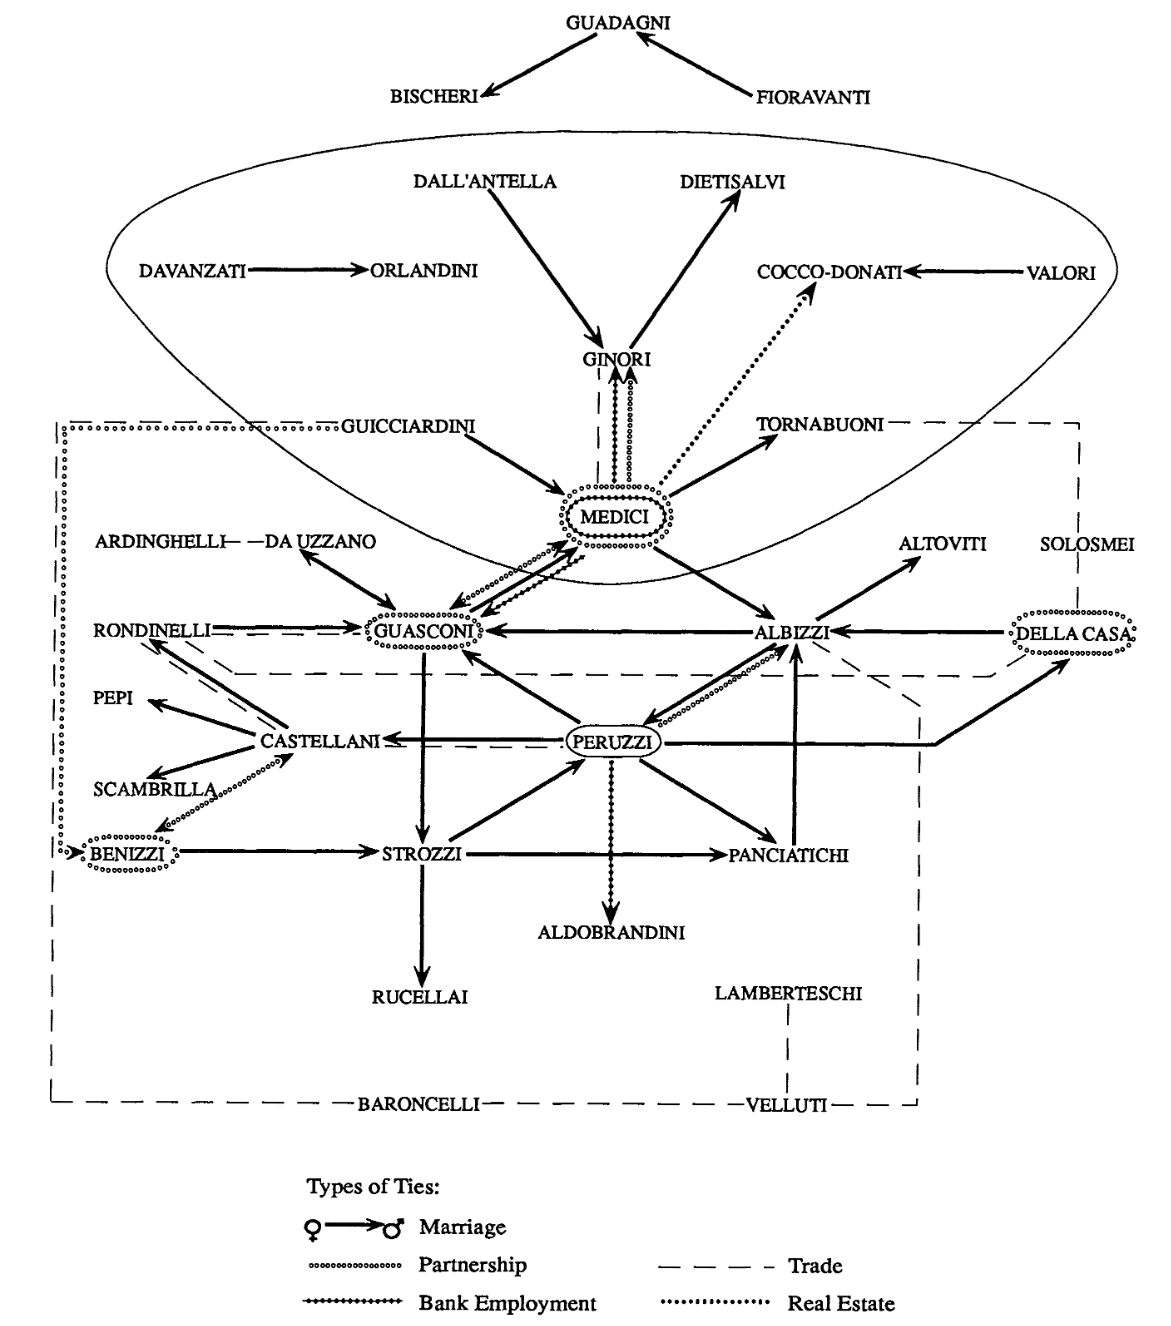
\includegraphics[width=0.8\textwidth]{static/figures/RelatedWork/padgett-Medicis.png}
    \caption{Marriage, partnership. trading, banking, and real estate networks of the powerful families of Florence from \cite{padgettRobustActionRise1993}. We can see the central position in the network of the Medici Family.}
    \label{fig:padgett-medicis}
\end{figure}

Several historians are using and continuously improving the HSNA methods which can be very effective to study relational historical phenomena~\cite{kerschbaumerPowerNetworksProspects2015}.
Moreover, historians rarely rely on a single approach when studying an era or phenomenon, they mix methods and tools from several domains of social and natural sciences with their own practices~\cite{padgettRobustActionRise1993, petzCombiningNetworkResearch2022}.




%However, constructing a network from historical sources, which can differ in their structure is not a trivial task.
%The most straightforward approach, based on the most well known social network analysis, consists in constructing social network based on simple graph $G = (V, E)$ with $V$ a set a vertices representing the persons of interest, and $E \subseteq V^2$ a set of edges modeling the social ties between pairs of persons.
%This allows to have a simple network to visualize and analyze, but does not always reflect the social complexity of the real relationships.
%More complex networks models have been proposed in SNA to be able to model more complex social relationships.


\subsection{Network Modeling}

Constructing a network from historical documents, which can vary tremendously in their formats and structures, is not a trivial task \cite{alkadi2022}.
The most straightforward and well-known approach consists in constructing a social network based on a simple graph $G = (V, E)$ with $V$ a set of vertices representing the actors of interest (very often individuals mentioned in the documents), and $E \subseteq V^2$ a set of edges modeling the social ties between pairs of actors.
This allows to have a simple network to visualize and analyze, but it does not always reflect the sociological complexity of information contained in the documents.
%More complex networks models have been proposed in SNA and HNR to be able to model more complex social relationships.
HSNA network models have evolved over time to better take into account concrete properties of social networks, such as types of actors using labeled networks, the importance of actors or relations with weighted networks, mixed relationships with multiplex networks, dynamics of relations with dynamic networks.
Bipartite networks have been proposed to model relations between two types of entities, such as organization and employees where the relations link employees to organizations but not employees to employees or organizations to organizations.
Many social situations or documents can be modeled in these terms (%\textit{Interlocking directorates},
affiliation lists or co-authoring).
Multivariate networks, \ie graphs, where vertices and edges can be assigned multiple ``properties'' or ``attributes'', are less used in SNA\@.
These attributes are often considered secondary, the emphasis of SNA being on the topology, its features, measures, and evolution.

Historians, demographers, sociologists, and anthropologists have also been designing specific data models for their social networks, based on genealogy or more generally kinship~\cite{hambergerKinshipNetworkAnalysis2011}.
For genealogy, the standard GEDCOM~\cite{gedcom} format models a genealogical graph as a bipartite graph with two types of vertices: individuals and families.
This format also integrates an ``event'' object but it is diversely adapted in genealogical tools.
The \href{https://www.kintip.net/}{Puck software} has extended its original genealogical graph with the concept of ``relational nodes'' to adapt the data model to more family structures and to integrate other social relationships for anthropology and historical studies~\cite{hambergerScanningPatternsRelationship2014}.






\section{Social Network Visualization}\label{sec:social-network-visualization}


Practitioners of SNA and HSNA have always visually depicted their networks for validation and communication purposes, mostly using node-link diagrams.
With the increase in average network size and density and the diversity of network models, new visualization techniques have been proposed to represent the diversity of studied networks.
Moreover, more and more social scientists are following exploratory approaches using Visual Analytics (VA) tools, to describe more in-depth their data and generate new interesting hypotheses, using interaction and exploration capabilities.

\subsection{Graph Drawing}

Sociologists rapidly saw the potential of graphically showing relationships between individuals, to better comprehend the underlying social structure and communicate their findings.
Moreno elaborated sociograms to visually show friendships among schoolchildren with circles and lines to respectively show children and friendships ties \cite{morenoWhoShallSurvive1934}.
This type of representation---commonly called node-link diagram---is the most widely used in social sciences, as it is rapidly understandable and effective for small to medium-sized networks which is usually the norm in social sciences.
The most used social network visual analytics software such as Gephi \cite{Gephi} and Pajek \cite{mrvarAnalysisVisualizationLarge2016} are based on this type of representation and allow a fully integrated exploration and analysis with the help of various algorithms.
Finding an optimal placement for the nodes is however not that simple as several metrics can be optimized depending on the desired drawing, such as the number of edge crossings, the variance of edge length, orthogonality of edges, etc~\cite{cristofoliPrincipesUsagesDessins, kosakAutomatingLayoutNetwork1994}. \autoref{fig:kosak-graph-drawing} shows some of these metrics, synthesized by Kosara and al.~\cite{kosakAutomatingLayoutNetwork1994}.
In \autoref{fig:moreno-sociogram} we can see the difference in readability between the original manual layout (left) and an automatic one (right).
Automatic layouts which aim at optimizing readability metrics give clearer diagrams.
The number of edge crossings is often considered the most important measure, but finding a drawing with the optimal number of crossings is an NP-Hard problem, meaning that heuristics are needed for most real-world use cases.
A large number of algorithms have been designed such as force-directed ones, modeling the nodes as particles that repulse each other and are attracted together when connected with a link that can be seen as strings.
Other visual techniques have been proposed to represent networks such as matrices, circular layouts, and arcs, but are less used in social sciences \cite{mcguffinSimpleAlgorithmsNetwork2012}.
Still, Matrices have been shown to be more effective than node-link diagrams for several tasks such as finding cluster-related patterns, especially for medium to large networks \cite{ghoniemComparisonReadabilityGraphs2004, abdelaalComparativeEvaluationBipartite2022}.

\begin{figure}
    \centering % avoid the use of \begin{center}...\end{center} and use \centering instead (more compact)
    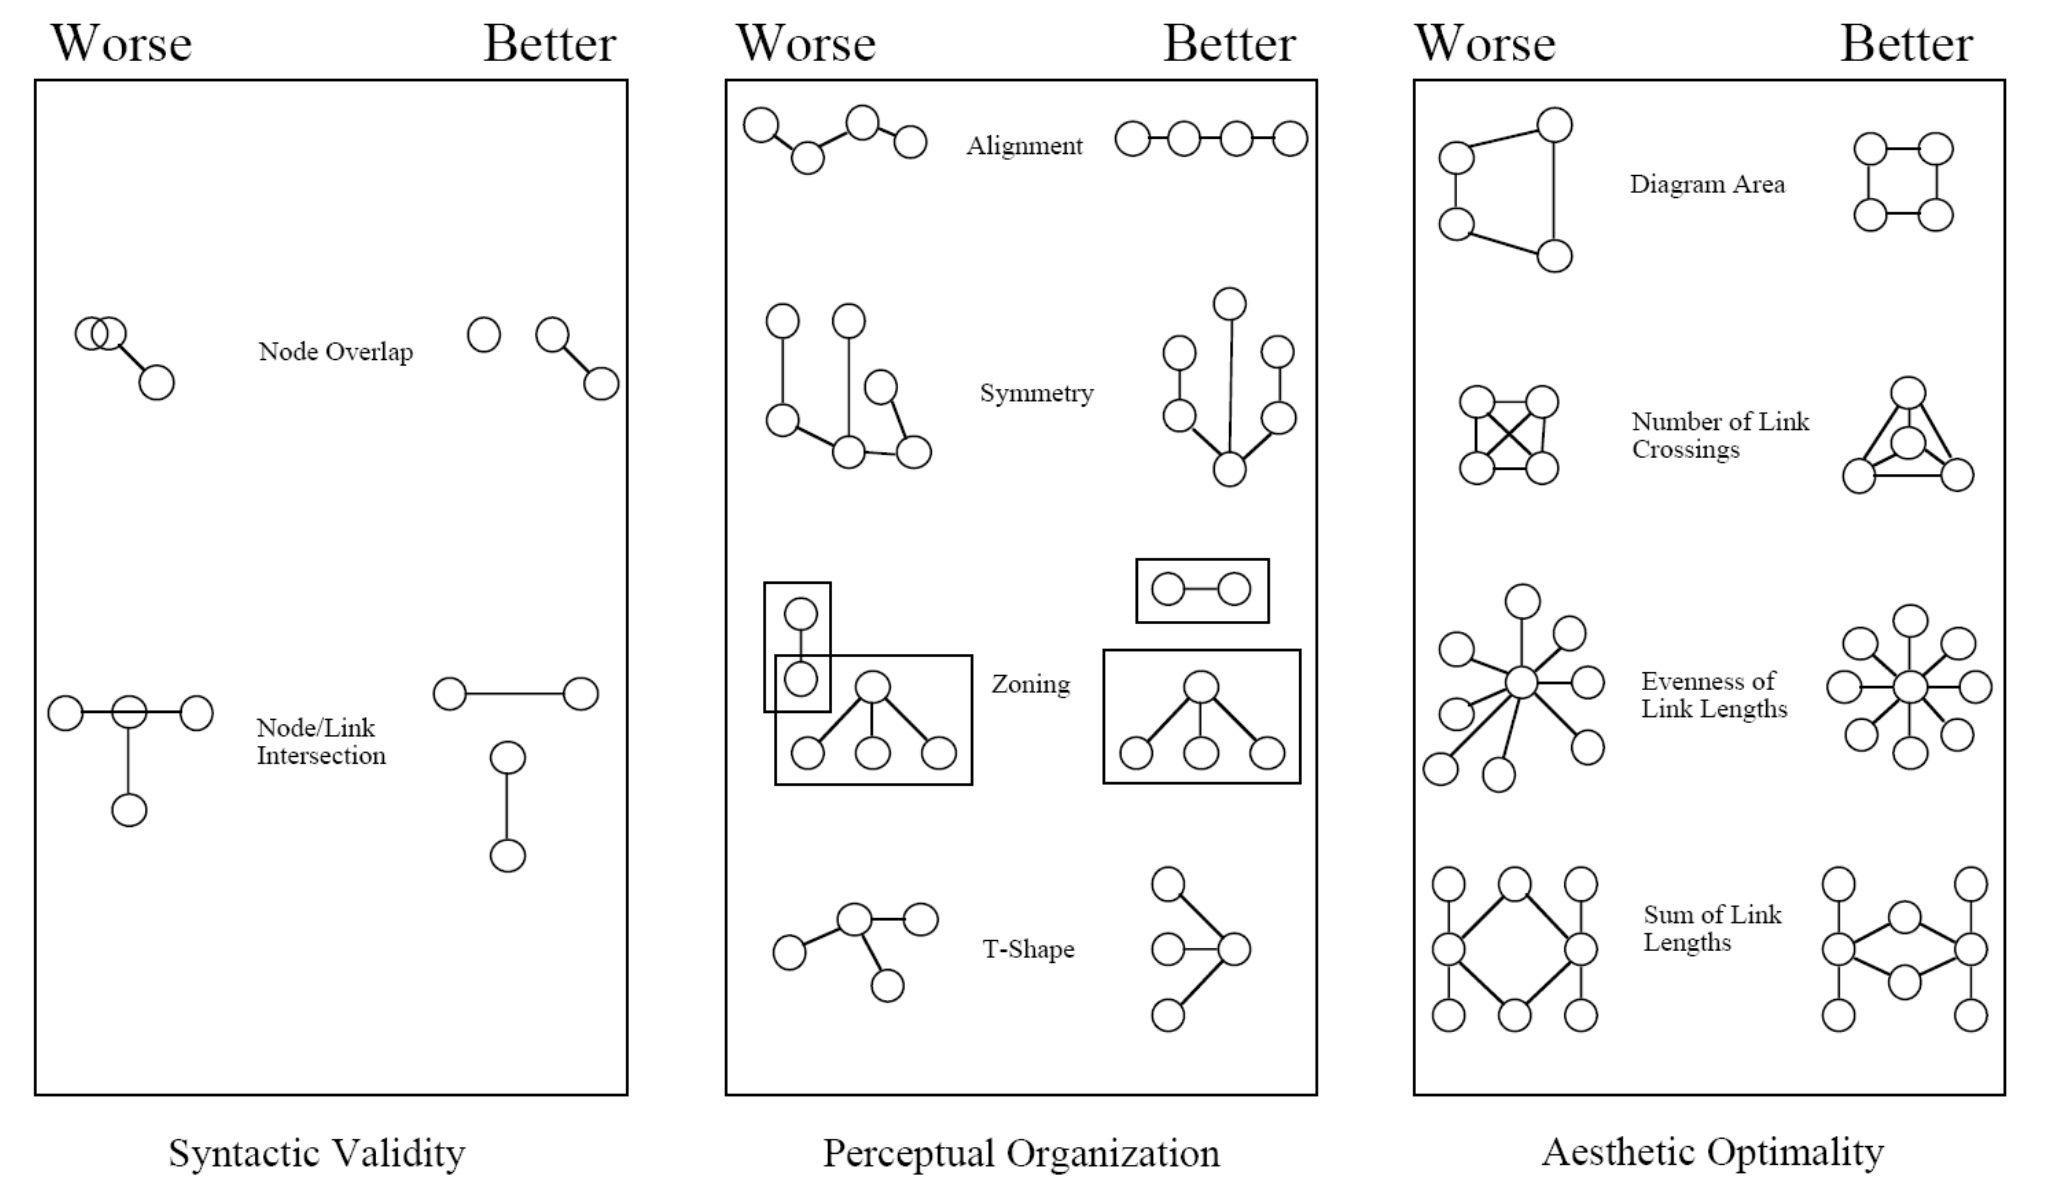
\includegraphics[width=1\textwidth]{static/figures/RelatedWork/Kosak-nodelinkdiagramMetrics}
    \caption{Different criteria are proposed to enhance node-link diagram readability. Image from \cite{kosakAutomatingLayoutNetwork1994}}
    \label{fig:kosak-graph-drawing}
\end{figure}

As social scientists are using more complex network models such as bipartite or temporal networks, more sophisticated representations are needed.
%The visualization community proposed new visualization systems for specific network types such as PAOHVis for temporal hypergraphs, NodeTrix for clustered networks or Juniper for Multivariate networks.
The visualization community developed new representations to visualize other network types such as dynamic hypergraphs with PAOHVis \cite{valdiviaAnalyzingDynamicHypergraphs2021}, clustered graphs with NodeTrix \cite{henryNodeTrixHybridVisualization2007} (illustrated in \autoref{fig:Riche-NodeTrix}), geolocated social networks with the Vistorian \cite{serranomolineroUnderstandingUseVistorian2017}, and multivariate networks with Juniper \cite{nobreJuniperTreeTable2019}.
However, these new network representations take time to be adopted by social scientists who rarely use those.


\begin{figure}
    \centering % avoid the use of \begin{center}...\end{center} and use \centering instead (more compact)
    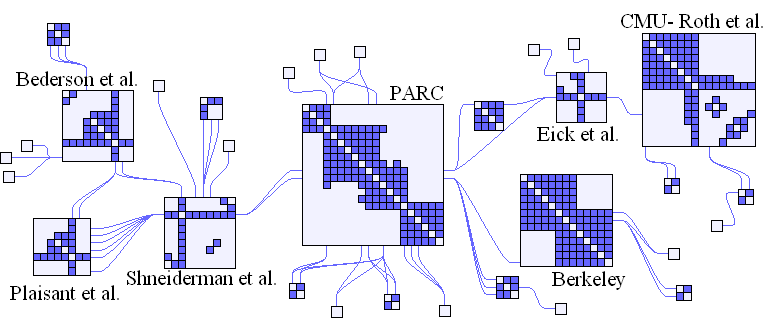
\includegraphics[width=0.8\textwidth]{static/figures/RelatedWork/NodeTrix.png}
    \caption{NodeTrix system showing a scientific collaboration social network with clusters. Each cluster is represented as a matrix,  Image from \cite{henryNodeTrixHybridVisualization2007}.}
    \label{fig:Riche-NodeTrix}
\end{figure}


\subsection{Social Network Visual Analytics}

Most widely used social network visualization softwares by social scientists are Gephi \cite{Gephi}, Pajek \cite{mrvarAnalysisVisualizationLarge2016}, and NodeXl \cite{NodeXL} which provide node-link diagrams, and allow basic interactions such as selection to explore the network.
These softwares usually provides automatic computation of several network measures such as the density and the diameter, allowing users to follow SNA workflows all in the interface.
Similarly, Automatic clustering capabilities are provided letting users find interesting community structure in their network.
\autoref{fig:gephi} presents the Gephi interface showing a clustered social network, where each node is part of a cluster, encoded by color.

\begin{figure}
    \centering % avoid the use of \begin{center}...\end{center} and use \centering instead (more compact)
    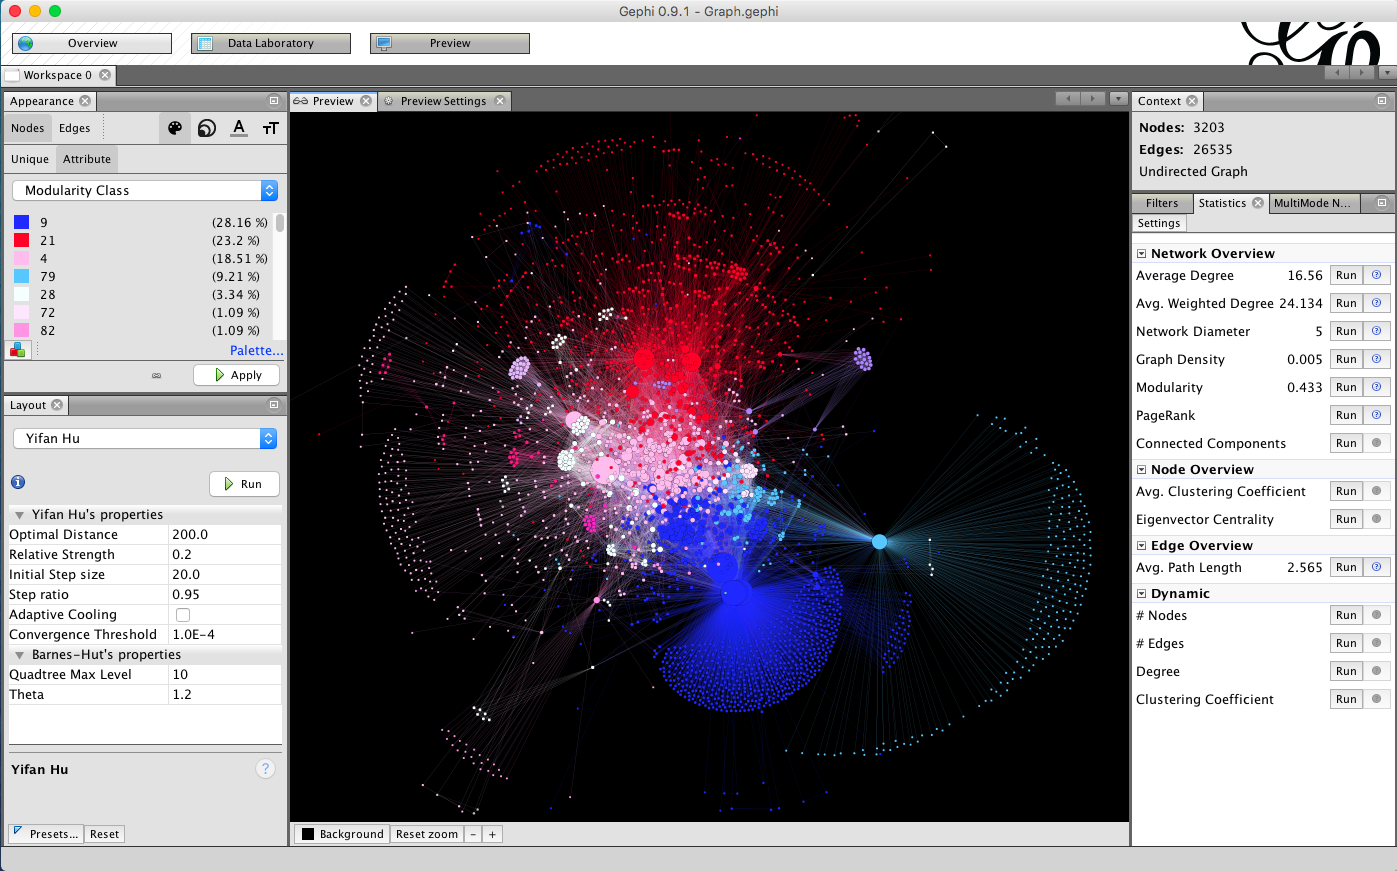
\includegraphics[width=0.8\textwidth]{static/figures/RelatedWork/Gephi_0.9.1_Network_Analysis_and_Visualization_Software}
    \caption{Gephi \cite{Gephi} interface. The network is represented with a node-link diagram. Users can interact on the visualization and encode node and links visual attribute (color, size etc.) with network measures computed directly in the interface, such as the node degree, or clustering results.}
    \label{fig:gephi}
\end{figure}
More complex VA interface have been proposed to explore social networks with complex interactions and more complex network models such as GUESS and the Vistorian.
These interfaces let social scientists explore their data with other interactions such as filtering, and often propose multiple coordinated views allowing to see the data through different lens.
For example, the Vistorian can show the data using a node-link diagram, a matrix, a map, and arc diagrams.
%These interfaces are usually aimed at more complex model than simple network,

Unfortunately, social scientists are often not trained in computer science and mathematical methods, and most of them have been frustrated by VA tools and by how it was guiding their analysis in predefined ways.
Interfaces leveraging automatic data mining algorithms sometimes put users in an awkward position, as they have a hard time interpreting results coming from those black-box algorithms.
They usually end up trying several algorithms until they stumble upon a satisfactory enough solution \cite{pisterIntegratingPriorKnowledge2021}.

Cleaning and importing the data is also complicated, as the annotation and network modeling process are not straightforward.
Thus, social scientists often encounter errors and inconsistencies in the data once they visualize it, that they want to correct.
It leads to continuous back and forth between their analysis process inside the VA tool they are using, and their original sources and annotation/modeling process, to correct errors or modify annotations.
Interestingly, the network model choice plays a crucial role in the process, as a simple network model representing only the persons (as it is often the case) will make it harder to trace back to the original documents containing the annotations from the network entities.
Yet the majority of Social Network VA systems enforce simple network models, making this retroactive process harder.
Some interfaces still incorporate data models encapsulating document representations, such as Jigsaw \cite{staskoJigsawSupportingInvestigative2008} which is a VA systems using textual documents as a data model, originally developed for intelligence analysis.
It allows an analysis of the documents and their mentions of entities (persons, locations, institutions, etc.) through multiple coordinated views.
Using such model allow to rapidly see errors and inconsistencies in the documents annotations, while still following complex analyzes.

Finally, more work is still to be done on social network VA tools, to provide more guidance and power to social scientists while doing their analysis, and to help them to do easier back and forth between their analysis and the annotation, network modeling, and cleaning steps, as they play a big role in the historian workflow.

































=======
Finally, more work is still to be done on social network VA tools, to provide more guidance and power to social scientists while doing their analysis, and to help them to do easier back and forth between their analysis and the annotation, network modeling, and cleaning steps, as they play a big role in the historian workflow.
>>>>>>> origin/overleaf-2022-09-13-0755

    \chapter{Historical Social Network Analysis Process, Pitfalls, and Network Modeling}\label{ch:hsna-process-and-network-modeling}
\minitoc

I describe in this chapter a formalization of the \hsna workflow followed by social historians, to shed light on their process and summarize recurring pitfalls to identify how \va could support them in this workflow.
Most \hsna practitioners report on their findings concerning the network they constructed from their sources, but few highlight the process which led to these conclusions from the raw historical documents, even though they have to make several encoding, modification, and modeling decisions that deeply influence the final analysis\cite{alkadi2022}.
Specifically, social historians can model documents and their content through various network models which have been proposed in the literature.
I discuss this step in depth as it impacts the annotation and analysis possibilities, and I give an answer to our first research question \qone by proposing to model this type of data with \modelplural.
This model satisfies \simplicity, \reality, and \traceability properties, which we define as critical for social history work from our joint collaborations with social historians and current critics of \hsna \cite{lemercier12FormalNetwork2015, lemercierBackSourcesPracticing2021, edelsteinHistoricalResearchDigital2017}.

\paperbox{This chapter is an updated version of an article presented at the VIS4DH workshop of the IEEE VIS: Visualization \& Visual Analytics Conference 2022 which is currently being published in IEEE Explore\cite{pisterHistoricalDocumentsSocial2022}. It was a collaboration with Nicole Dufournaud, Pascal Cristofoli, and my supervisors Christophe Prieur and Jean-Daniel Fekete. I have been leading the discussions, elaboration of concepts, and writing of the paper.}

\section{Context}

Tools for social network visualization tend to ignore the context in which the networks are produced, where they come from, and the workflow that led from their origin (e.g., documents, polls, interviews, web scraping) to their network form.
Yet, practitioners of social history need to inspect and encode their sources in depth using ad hoc methods to generate a network, and sometimes end with errors or simple networks which do not fit their analysis goals\cite{lemercierQuantitativeMethodsHumanities2019}.
%Yet, practitioners of social history need to generate many networks from the same documents/sources to visualize and analyze them
% and need to maintain the provenance from documents to analyzes and back.
% In this article, we explain why and how effective tools for supporting Historical Social Network Analysis~\cite{wetherell_historical_1998} (HSNA) should model social networks in multiple steps to support three essential principles: \traceability, connection to \emph{reality}, and \simplicity.
In this chapter, after describing and characterizing the workflow of \hsna~\cite{wetherellHistoricalSocialNetwork1998} from our collaborations with social historians, I explain why and how effective tools for supporting this process should model social networks in multiple steps to support three essential principles: \traceability, \reality, and \simplicity.
These principles emerged from joint experiences as historians and computer scientists were collaborating on multiple projects, and aim at simplifying the \hsna process while enhancing exploration and analysis options and replicability.
%These principles emerged from joint experiences as historians and computer scientists while collaborating on multiple projects, and aim at simplifying the \hsna process while enhancing exploration and analysis options and replicability.

Social historians' goal is to characterize socio-economic phenomena and their dynamics in a restricted period and place of interest and to see how individual people of that time lived through those changes\cite{tilly1984retrieving}.
For this, they rely on historical documents that they inspect in depth to next extract qualitative and quantitative information allowing them to answer their research questions.

%They typically extract qualitative and quantitative information from an identified corpus of documents, to then make conclusions on socio-economic topics such as migrations, business dynamics, education, and kinship.
%For doing this, historians can apply Social Network Analysis (SNA), a method---sometimes referred to as a paradigm---which consists in modeling the social relationships between a set of entities---usually individuals---into a network.
%Much work has been done to adapt SNA to the context of historical document exploitation, and although several approaches coexist they can be brought together under the banner of Historical Social Network Analysis~\cite{wetherellHistoricalSocialNetwork1998} (HSNA) or Historical Network Research~\cite{kerschbaumerPowerNetworksProspects2015} (HNR).
To study relational social structures where individuals influence each other such as families, companies, and institutions, historians rely on \hsna by modeling the social relationships between a set of entities---usually individuals---into a network.
%Historians therefore collect documents, annotate them, construct a network from the annotations that they finally analyze and visualize to understand the structural aspect of their object of study by validating and/or generating new hypotheses.
However, the process leading to the final network from the raw documents is often linear, and it is common that, when visualizing their network, historians spot errors and inconsistencies in the network structure that they could have fixed if the process was more iterative\cite{alkadi2022}.
Moreover, historical documents are often complex, meaning that the annotation and modeling process can be done in many different ways, concerning what to annotate from the documents\cite{lemercierBackSourcesPracticing2021} and how to model the annotation in a network\cite{cristofoliAuxSourcesGrands2008}.
Several network models have been proposed ranging from simple and specific ones like co-occurrence networks to more general and complex ones such as multilayer networks and knowledge graphs.
Simple models allow answering specific questions and are easy to manipulate but are often too simplistic and may distort the information contained in the documents.
Moreover, they often break the traceability from the analysis to the original documents, making the communication of findings less reproducible and the process of modifying/correcting annotations complicated.
Indeed, errors and mismatches often occur in the annotation process, for example, due to entity disambiguation problems\cite{diesnerImpactEntityDisambiguation2015}.
On the contrary, too complex models are complicated to visualize and analyze, and historians do not always have the tools to create them properly.
In this chapter, I answer \qone (how to model historical documents into analyzable networks with the right balance between expressivity and simplicity) by proposing to model historical documents as \modelplural, where both persons and documents are modeled as nodes with attributes and the links represent both individuals' mentions in the documents and their social roles in the event witnessed by the documents (such as witness in a marriage act).
While this model is simple enough for creation and inspection, it allows tracing back the entities of the network to the original sources for a continuous annotation process and still accurately models the social relationships mentioned in the documents.
Historians can therefore use this model to simultaneously find errors and inconsistencies in their annotation process---allowing them easier back and forth between the annotation and analysis steps---while starting a first analysis and exploration of the data to answer their sociological questions.
The traceability to the original sources also makes the communication of findings more replicable and transparent.

% Very often, historians model the persons mentioned in the text as the nodes of the network, who are connected two by two by links modeling social relationships, such as friendships and family ties.
% However, historical documents are often rich in information and can refer to complex relationships involving more than two persons at the same time. Persons can also have different implications or roles in the documents, and relationships are often non symmetrical~\cite{lemercier_analyse_2005}.
% For example, there have been several studies on business documents concerning financial transactions~\cite{rossi_exploration_2014, crailsheimSpanishConnectionFrench2016}. These documents often involve more than two persons, who can have  different roles; this type of documents refer to sellers and buyers, but can also indicate other roles such as a guarantor, witness, or notary. These complex relationships are hard to model into simple person-to-person networks.
% Furthermore, textual sources almost always contain extra information in regard of the event they refer to like the date and time, location, and other such as the type and amount of the transactions. It can also contain extra information about the persons such as their job, family, and gender.
% It is clear that such information-rich data is difficultly modeled as a simple person-to-person network. Yet, even if more complex models have been proposed in the literature such as dynamic and bipartite networks, simple networks are still the most widespread model supported by popular tools.
% Moreover, a large number of HSNA studies focus on reporting network analysis results, but rarely give details on the encoding, annotation, and network modeling process even though these are primordial steps which influence greatly the final results. Therefore, it can be difficult for readers to trace back the analysis to the original documents, and can pose replicability problems~\cite{baker_1500_2016}. For these reasons, network models that can more faithfully represent the complex reality of the documents while allowing traceability to the sources and are easy enough to manipulate are needed.
% In this paper, we first describe the HSNA work process that we have observed from the literature and collaborations, starting from the textual sources acquisition to the analysis and visualization of the network, and we identify potential issues related to analysis for each step.
% Then, after describing the most used network models in HSNA, we formalize a network model which satisfies \textit{reality} and \traceability properties, and
% which models well the majority of historical sources we encountered with their complexity: the \model. We give real world examples on how this model has been used to follow HSNA pipelines, from data preparation to visual analysis using a visual query system. From these examples, we identify three problems which arise when doing a network projection but not when using \modelplural: no loss of information, no duplication, and no distortion.

%
%\section{Related Work}
%
%Since we already elaborated on the related work of SNA, HNR, network modeling, and social network visualization in \autoref{ch:related-work}, we only discuss in this section the related work concerning historians' workflow and methodology descriptions.
%
%The essence of the historical discipline is based on a critical approach of sources and involves considering peers' work.
%Traditional approaches to history often focus on the construction of a narrative, without necessarily adopting a systematic and problematized approach to the exploitation of original sources.
%Social history and the ``Annales School'' proposed a new approach to history, by trying to describe and characterize socio-economic phenomena of the past by rigorously extracting information from historical documents and making conclusions from them.
%
%
%
%With similar aims, Glaser and Strauss developed the ``Grounded Theory''~\cite{glaserDiscoveryGroundedTheory2010} as a methodology for the humanities to build hypotheses and theories by solely studying and categorizing real-world observations, without starting from prior knowledge and predefined categories.
%Later on in the 1960s, quantitative methods started to be used in history, providing statistical and later computer-supported tools to aid historians in grounding their analysis in mathematical models and results.
%Unfortunately, the lack of methodology and understanding between the two worlds led to many criticisms by historians pointing to using wrong metrics, simplifying categories, and disconnections between the original documents and analysis~\cite{karila-cohenNouvellesCuisinesHistoire2018, lemercierBackSourcesPracticing2021}.
%Quantitative history has been showed to be useful when used properly and when not focusing only on numbers, and several books have been published on how to efficiently use statistical methods such as summarizations, correlations, statistical distributions, statistical testing, time series etc.~\cite{hudsonHistoryNumbersIntroduction2016, lemercierQuantitativeMethodsHumanities2019}.
%Similarly, the use of network science for historical aims increased in recent years, and a lot or resources exist on how to use network methods and measures for historical research~\cite{lemercier12FormalNetwork2015, kerschbaumerPowerNetworksProspects2015}.
%
%However, little work has been done on describing and formalizing the process before the analysis part for a quantitative and network research workflow.
%Indeed, if it is central to know how to manipulate statistical and network concepts and methods when following this kind of methodology, it is as important if not even more to follow a correct and rigorous workflow to generate the data we plan to analyze beforehand.
%The process to generate a clean quantitative or network dataset from historical sources is difficult and requires several data acquisition, annotation, and cleaning steps.
%Social analysts are not always trained on how to do these steps effectivity, which can lead to errors, inconsistencies, and mismatches between the chosen data models and the historical questions~\cite{alkadi2022}.
%Karila-Cohen and al.\ provide some advice on how to annotate historical documents with the aim of using quantitative methods~\cite{karila-cohenNouvellesCuisinesHistoire2018} and prone that the annotation and analytical processes should not be dispatched between several persons, as both usually influence each other.
%Dufournaud describes her workflow in depth when studying the socio-economic status of women in France in the 16th and 17th centuries, which she splits into three steps: \textit{data collection}, \textit{data processing}, and \textit{data analysis}~\cite{dufournaudCommentRendreVisible2018}.
%She provides the tools and methodology she used to annotate her data, providing transparency on her historical analysis and methodological resources.
%Cristofoli discusses the network modeling problem when following an HSNA and highlights the fact that the same historical documents can be modeled in different ways~\cite{cristofoliAuxSourcesGrands2008}.
%Historians should be aware of this and choose a network model which fits their analytical goals.



\section{Related Work}

Since I already elaborated on the related work of SNA, network modeling, and social network visualization in \autoref{ch:related-work}, I only discuss in this section the related work concerning historians' methodology and workflows.

%\subsection{Methodologies and formalisms}

\subsection{History Methodology}

%The essence of the historical discipline is based on a critical approach of sources and involves considering peers' work.
%Traditional approaches to history often focus on the construction of a narrative, without necessarily adopting a systematic and problematized approach to the exploitation of an exhaustive set of historical documents.
%Social history and the ``Annales School'' shifted the focus from a narrative approach of History focused on individuals, towards exhaustive inspection of documents to make sociological conclusions on groups and organizations.
%Historians therefore started to extract numbers and categories from their sources to point to social and economical aspects of societies. \todo{example}
%This type of practice logically led historians to use quantitative methods with the rise of computer science in the 1960s.


The essence of the historical discipline is based on a critical approach to sources and involves considering peers' work.
Traditional approaches to history often focus on the construction of a narrative, without necessarily adopting a systematic and problematized approach to the exploitation of an exhaustive set of historical documents\cite{tillyObservationsSocialProcesses2004}.
With the development of social and quantitative history, historians now have a panoply of methods to exhaustively extract quantitative data from their sources and analyze it to ground their results in verifiable claims.
Many historians criticized this computational aspect of history\cite{lepetitHistoireQuantitativeDeux1989, fogelLimitsQuantitativeMethods1975, barnesBigDataLittle2013}, pointing out that it would lead to errors and missing the core content of historical sources.
However, using quantitative approaches and formalisms is not exclusive to having a deep understanding of the documents and their context, nor building a narrative on top of their quantitative analysis.
Good historical work can in fact be described as a combination of the two \cite{karila-cohenNouvellesCuisinesHistoire2018}, as Tilly says ``Formalisms play their parts in the space between the initial collection of archival material and the final production of narratives. In my own historical research, formalisms figure prominently from early in the ordering of evidence to late in its analysis; \textup{[\,\dots]} As it happens, many other historians rush from sources to reasoned narratives without pausing to employ formalisms, or even to reflect very self-consciously on the logical structure of their arguments, hence on what the evidence should show if their arguments are correct'' \cite{tillyObservationsSocialProcesses2004}.
Historians have a panoply of methods and formalisms they can leverage to ground their narratives in concrete comparable results, such as serial analysis, tabular analysis, classical statistical treatments, and network analysis.

However, formalisms have to be used wisely and with a critical vision of the documents and their context, so as to not fall into simplifications, anachronisms, and errors which are pertinent critics of quantitative history\cite{lemercierQuantitativeMethodsHumanities2019, lemercierBackSourcesPracticing2021}.
%Such formalisms often demand categorization and aggregation of the original documents, which can result in distortion and simplification of the original documents content \cite{lemercierQuantitativeMethodsHumanities2019}.
Most historical work leverage several methods in the same study to support their claims through different qualitative and quantitative results \cite{petzCombiningNetworkResearch2022}.
The level of the plausibility of a claim increase or decrease depending on if the different evidence point to similar results or not.
%If several different evidence point to the same fact, the level of plausibility of the claim increase, even without uing formal statistical testing.
Similarly, historians often work on small populations or specific individuals---as it is the case with microhistory studies\cite{ginzburgMicrohistoire1981}---which can result in complications for generalization.
Only after studying several similar individuals or groups, historians are able to generalize and point to exceptions.
For example, by comparing several Jewish commercial communities in Europe during the first half of the 18th century, Trivellato has been able to generalize what is common to those groups (they have been trading between them and with outer ethnic groups) and what is specific to each (such as their business strategies) \cite{trivellatoThereFutureItalian2011}.
%Most historical work do not go to the level of statistical testing to verify their claims, but often combine several formalisms with a narrative to refute or support a hypothesis.
%As the objects of study are often on small to medium groups, the combination of several studies lead to the increase or decrease of level of plausibility of different claims.


%\todo{Grounded Theory}



\subsection{Historian Workflows}

%Many approaches have been introduced to analyze historical documents through various formalisms to analyze their content through quantification.
Many quantitative methods and formalisms are available for historians to inspect their sources with the aim of making historical claims.
Several textbooks describe and explain to social scientists and students who do not have formal computer science training in what consist these methods (statistical regression, Chi-squared test, network analysis, etc.) and how to practically use those with software and programming language \cite{archdeaconCorrelationRegressionAnalysis1994, floudIntroductionQuantitativeMethods2013}.
However, the process leading from the sources to the numeric artifacts (a table, a network, a timeline) has not been described thoroughly in the literature, especially with concrete examples, and is often not presented in scientific publications of concrete use cases.
Yet, the process leading from the documents to analyzable data requires social historians to make several annotations, encoding, and modeling decisions, concerning \emph{what} to extract from the source and \emph{how} to encode it.
This process is tedious and requires data acquisition, annotation, encoding, and modification with continuous back and forth between the different steps \cite{alkadi2022}.
%The process to generate a clean quantitative or network dataset from historical sources is difficult and requires several data acquisition, annotation, and cleaning steps.
%Social analysts are not always trained on how to do these steps effectivity, which can lead to errors, inconsistencies, and mismatches between the chosen data models and the historical questions~\cite{alkadi2022}.
This is a critical process as it can lead to simplifications, anachronism, distortion, or data that do not allow to answer original or new hypotheses \cite{karila-cohenNouvellesCuisinesHistoire2018, lemercierQuantitativeMethodsHumanities2019}.
Lemercier et al. give guidelines on how to encode information from historical documents to prevent introducing bias, by having a critical view of the documents \cite{lemercierBackSourcesPracticing2021}.
They emphasize the importance of the input phase of research and advise copying the first documents by hand while characterizing them in the most exhaustive and factual way, without imposing categorization.
This explorative step lets historians familiarize themselves with the content of the document, leading to a better view of what to encode to answer their research questions and sometimes to the formulation of new hypotheses.
For example, in their project on the social and geographical trajectories of Jews in Lubartów\cite{zakrzewski1932PopulationRegister2020}, a village in Poland, the team encoded the mean of writing inside the register documents (pen, pencil, ink, etc.) they were inspecting.
This information  allowed them to conclude that the inscription ``expelled'' written in pencil was probably added during World War II by Germans to denote exported Jews in the extermination camps.
When applying network analysis, historians often create specific person-to-person networks which allow them to answer precise research questions, but often lose this type of document-related information.
% If historians decide to apply network analysis, they also have to decide how to model their network, based on the entities they can extract from their documents and their research questions.
Cristofoli discusses the network modeling problem when following a network analysis and highlights the fact that the same historical documents can be modeled in different ways~\cite{cristofoliAuxSourcesGrands2008}, which can result in mismatches between the network shape and the research questions.
Dufournaud presents her quantitative and network workflow when studying the economic role of women during the 16\ts{th} and 17\ts{th} centuries in the city of Nantes, which she splits into three steps: data collection, data processing, and data analysis \cite{dufournaudCommentRendreVisible2018}.







%With similar aims, Glaser and Strauss developed the ``Grounded Theory''~\cite{glaserDiscoveryGroundedTheory2010} as a methodology for the humanities to build hypotheses and theories by solely studying and categorizing real-world observations, without starting from prior knowledge and predefined categories.
%Later on in the 1960s, quantitative methods started to be used in history, providing statistical and later computer-supported tools to aid historians in grounding their analysis in mathematical models and results.
%Unfortunately, the lack of methodology and understanding between the two worlds led to many criticisms by historians pointing to using wrong metrics, simplifying categories, and disconnections between the original documents and analysis~\cite{karila-cohenNouvellesCuisinesHistoire2018, lemercierBackSourcesPracticing2021}.
%Quantitative history has been showed to be useful when used properly and when not focusing only on numbers, and several books have been published on how to efficiently use statistical methods such as summarizations, correlations, statistical distributions, statistical testing, time series etc.~\cite{hudsonHistoryNumbersIntroduction2016, lemercierQuantitativeMethodsHumanities2019}.
%Similarly, the use of network science for historical aims increased in recent years, and a lot or resources exist on how to use network methods and measures for historical research~\cite{lemercier12FormalNetwork2015, kerschbaumerPowerNetworksProspects2015}.
%
%However, little work has been done on describing and formalizing the process before the analysis part for a quantitative and network research workflow.
%Indeed, if it is central to know how to manipulate statistical and network concepts and methods when following this kind of methodology, it is as important if not even more to follow a correct and rigorous workflow to generate the data we plan to analyze beforehand.
%The process to generate a clean quantitative or network dataset from historical sources is difficult and requires several data acquisition, annotation, and cleaning steps.
%Social analysts are not always trained on how to do these steps effectivity, which can lead to errors, inconsistencies, and mismatches between the chosen data models and the historical questions~\cite{alkadi2022}.
%Karila-Cohen and al.\ provide some advice on how to annotate historical documents with the aim of using quantitative methods~\cite{karila-cohenNouvellesCuisinesHistoire2018} and prone that the annotation and analytical processes should not be dispatched between several persons, as both usually influence each other.
%Dufournaud describes her workflow in depth when studying the socio-economic status of women in France in the 16th and 17th centuries, which she splits into three steps: \textit{data collection}, \textit{data processing}, and \textit{data analysis}~\cite{dufournaudCommentRendreVisible2018}.
%She provides the tools and methodology she used to annotate her data, providing transparency on her historical analysis and methodological resources.
%Cristofoli discusses the network modeling problem when following an HSNA and highlights the fact that the same historical documents can be modeled in different ways~\cite{cristofoliAuxSourcesGrands2008}.
%Historians should be aware of this and choose a network model which fits their analytical goals.


\section{Historical Social Network Analysis Workflow}\label{sec:hsna-workflow}


From the literature and our own projects of \hsna we conducted during the last three years in collaborations with social historians, I propose a formalization of the \hsna workflow divided into 5 steps: \textit{textual sources acquisition}, \textit{digitization}, \textit{annotation}, \textit{network creation}, and finally, \textit{visualization and analysis}.
I start by describing the sources and research questions of the different collaborations in \autoref{subsec:hsna-examples}, then explain each step of the workflow in \autoref{subsec:hsna-workflow}, and characterize three properties \va systems supporting this workflow should satisfy in \autoref{subsec:hsna-properties}.
%The workflow is presented in \autoref{fig:HSNA-process} along with potential and recurrent pitfalls.


\subsection{Examples}\label{subsec:hsna-examples}

We discussed with four experienced social historians collaborators at different steps of their \hsna workflow about their process: how they inspect and annotate their sources, what network representation they plan to use, and what are their research questions.
%annotation process and how they wanted to model their data into a network.
They all work on semi-structured historical documents, mentioning complex relationships.
I provide more details in the following:

\begin{enumerate}[nosep,leftmargin=*]
    \item Analysis of the social dynamics from \textbf{construction contracts in Italy in the 18\ts{th} century\cite{Cristofoli2018, Rolla2018}.}
    %\textcolor{red}{PC: The corpus was created by N. Rolla through the exploitation of the manuscript registers of the \textit{Azienda generale fabbriche e fortificazioni} (State Archives of Turin)[REF : Rolla Nicoletta, 2018, "Mobilité et conflits. Travailler sur les chantiers de construction piémontais dans la première moitié du XVIIIe siècle" dans Andrea Caracausi et Marco Schnyder (eds.), Travail et mobilité en Europe (XVIe-XIXe siècles), Villeneuve d’Ascq, Presses universitaires du Septentrion (coll. Histoire et civilisations), p. 49‑72]. }
    The corpus is made of contracts for different types of constructions in the Piedmont area in Italy. People are typically mentioned under three different construction roles: \textit{Associates} who are in charge of the construction, \textit{Guarantors} who bring financial guarantees, and \textit{Approvers}, who vouch for the guarantors. Documents contain information about the building sites, the types and materials of constructions, and the origins of people. Historians working on this project were interested in characterizing the social structure underlying those contracts, if there were specializations in types of construction, and describing the life trajectory of certain people.
    \item Analysis of migrations from the \textbf{genealogy of a French family between the 17\ts{th}--20\ts{th} centuries} [unpublished work].
    The corpus is made of family trees referring to several document/event types: birth and death certificates, marriage acts, military records, and census reports.
    The social historian wants to characterize the main migrations of individuals and families in France, according to time and place.
    She is also interested in studying specific families, with theories that, in some areas, people were moving places in a circular fashion over the years.
    Finally, she is interested in the average social mobility of individuals across the years.
%    The roles are different for each event type and consist of \textit{children, father, mother} for the birth events, \textit{deceased} for the death event, \textit{spouse} and \textit{witnesses} for the marriages, and \textit{family member}s for the census events.
    \item Analysis of \textbf{marriage acts in Buenos Aires in the 17--19\ts{th} centuries ~\cite{moutoukiasBuenosAiresPort2016, rueda1989matrimonios}.}
% \textcolor{red}{PC: The corpus was created by Z. Moutoukias \& C. Prieur through the digitization and annotation of a publication of the Buenos Aires Archives [REF: Jauregui Rueda, Carlos, Matrimonios de la catedral de Buenos Aires, 1747 – 1823, Buenos Aires, Fuentes Genealógicas e Históricas Argentinas, 1989]. }
    The corpus is made of summaries of marriage records that mention the spouses and the witnesses of the wedding.
    The origin, date of birth, and parents' names are specified for both spouses.
    The historian is mainly interested in characterizing the relationships between witnesses and spouses---if they are typically from the same family, and if being a witness is sometimes used to ask favors in exchange.
    % These parenting relationships are important for our collaborator, but do not refer to the same event as the marriage. Thus, we create another event node referencing the birth event, with \textit{father, mother}, \textit{child} as roles and the associated birth year and location as node attributes.
    \item Socio-political analysis of \textbf{Germans ethnic migration from communist Romania to West Germany in the 20th century (ongoing work)~\cite{diminescuMigrationEthnicGermans2020}.}
    The corpus is made of administrative forms that mention persons requesting to migrate, along with the persons they want to join, and the administrative persons of the ministry in charge of the forms.
    The family members of the aspiring migrants are also mentioned in the forms, with their respective dates of birth.
    Our historian collaborator is interested in characterizing the socio-economical profile of migrants and the types of family members they are typically joining in Germany.
\end{enumerate}

Each historian planned to follow a network analysis.
They typically first read and inspect their sources in depth, before encoding their content with the aim of constructing a network.
They plan to use analytical and visualization tools to then explore the structure of the relationships, and answer their questions.

\subsection{Workflow}\label{subsec:hsna-workflow}

\begin{figure}
%    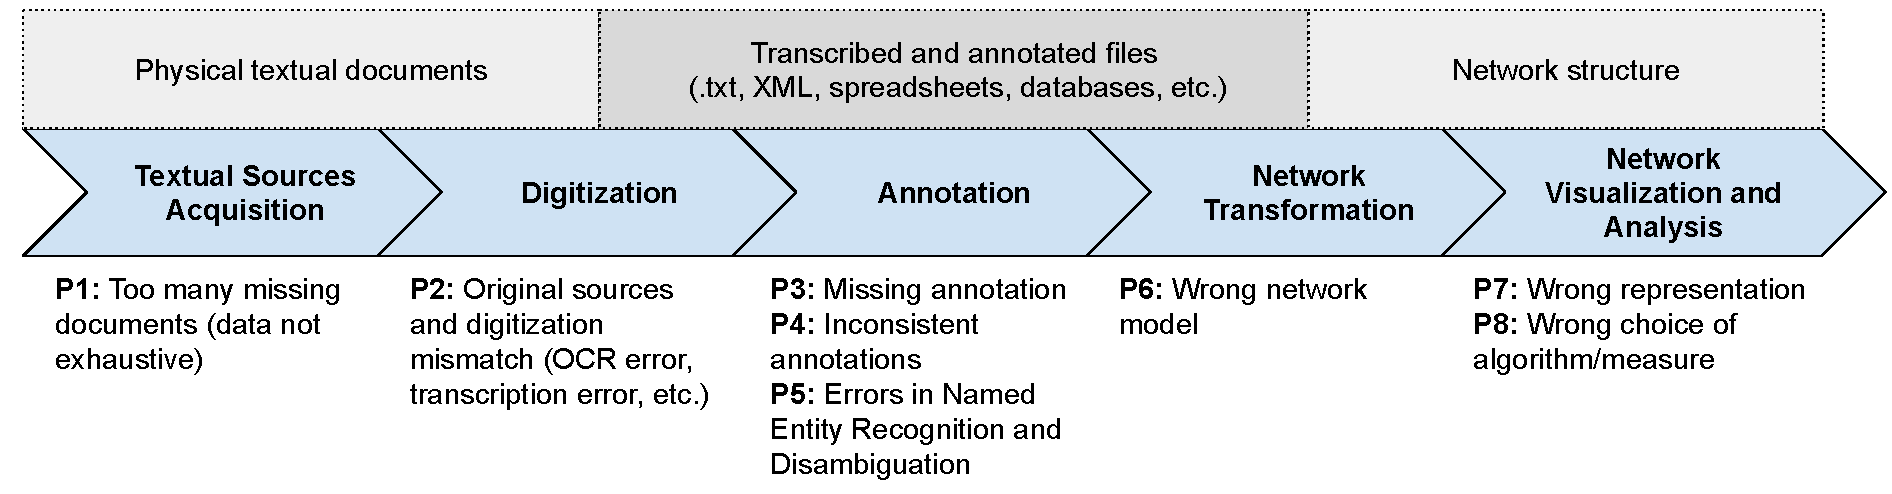
\includegraphics[origin=c, width=\textwidth]{static/figures/HSNAProcess/OriginalPaperFigures/Process5.pdf}
    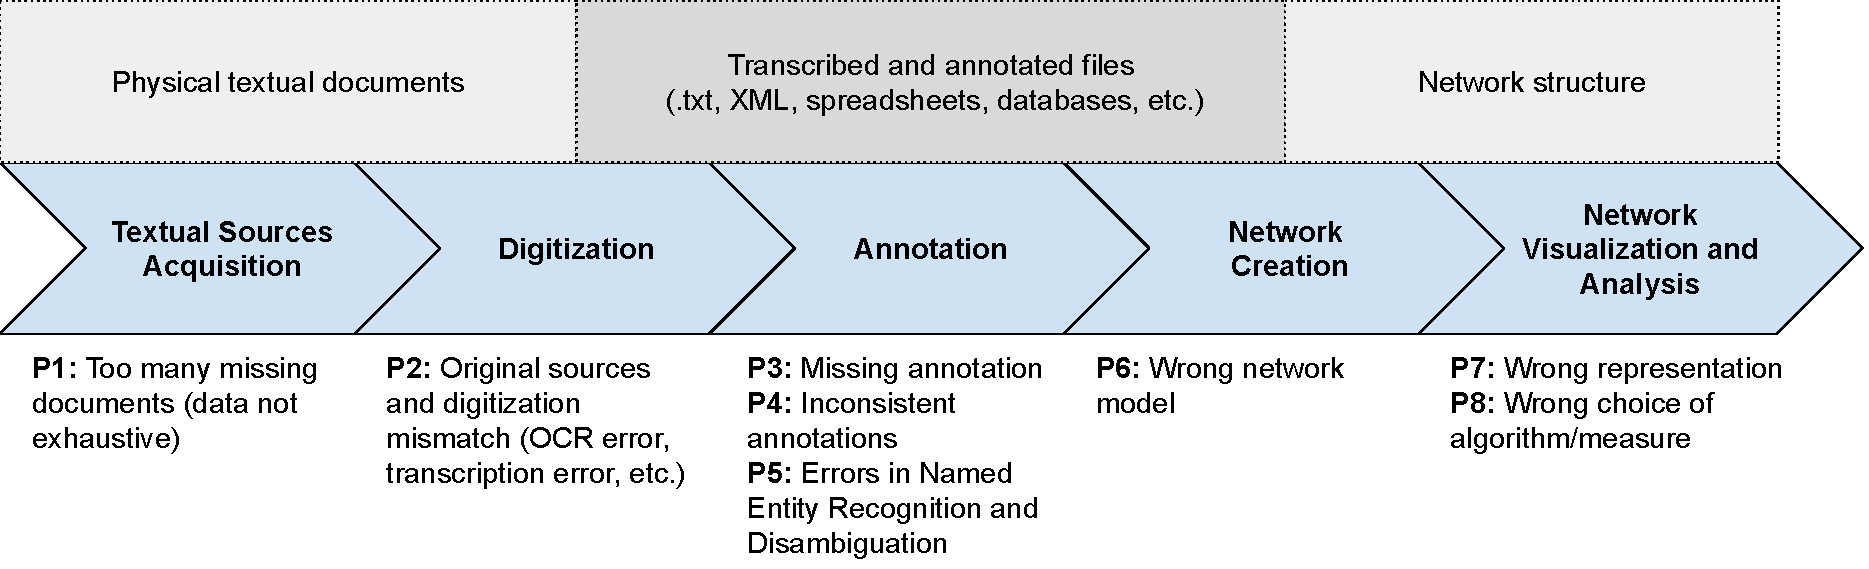
\includegraphics[origin=c, width=\textwidth]{static/figures/HSNAProcess/process.pdf}
    \caption{HSNA workflow is split into five steps: textual sources acquisition, digitization, annotation, network creation, and network visualization/analysis. Practitioners typically have to do back and forth during the process. I list potential pitfalls for each step.}
    \label{fig:HSNA-process}
\end{figure}

% This process is not straightforward, and has not been discussed a lot in the HSNA community. Dufournaud describes her workflow when studying socio-economic status of women in France in the 16th and 17th centuries, that she split in three steps: \textit{data collection}, \textit{data processing}, and \textit{data analysis}~\cite{dufournaud2018comment}. From the literature and discussions with historians collaborators we propose an HSNA workflow description split in 5 steps: \textit{textual sources acquisition}, \textit{digitization}, \textit{annotation}, \textit{network creation} and finally \textit{visualization and analysis}. The workflow is presented in \autoref{fig:HSNA-process} along recurrent potential issues which can arise.
%\noindent\textbf{Textual Sources Acquisition}

I formalize the \hsna workflow of social historians from our collaborations (\autoref{subsec:hsna-examples}) but also the literature, and informal discussions with other social historians.
We can divide it into 5 steps: \textit{textual sources acquisition}, \textit{digitization}, \textit{annotation}, \textit{network creation}, and finally, \textit{visualization and analysis}.
For each step, I present recurring pitfalls which occurred during our collaborations, or that are discussed in the literature\cite{diesnerImpactEntityDisambiguation2015, cristofoliAuxSourcesGrands2008, lemercierAnalyseReseauxHistoire2005}.
A diagram of the workflow is presented in \autoref{fig:HSNA-process}.

%\subsubsection{Textual Sources Acquisition}
\noindent\textbf{Textual Sources Acquisition}
Historians' first step is gathering a set of textual historical documents mentioning people with whom they will have social ties.
For this, they usually take documents from a specific source---such as a folder from a national or local archive---and restrict them to a period and place that they want to study.
They also often restrict themselves to one document type---such as marriage or notary acts---to focus the analysis on one or a few types of social relationships that they want to understand in depth.
However, one rule of the historian's method is to crosscheck from multiple sources, so an initial corpus is often extended with another set of related sources.
Once they restricted their search to a set of documents, a time, and a geographic area, they try to exhaustively find all the documents matching the desired properties, as \textbf{missing documents can result in uncertainty in the network structure and, therefore, the sociological conclusions (P1)}.

%\subsubsection{Digitization}
\noindent\textbf{Digitization}
Digitization consists in converting the sources into a digital format.
% \textcolor{green}{For modern history where the documents have been produced digitally or scanned and digitized through optical character recognition (OCR), this step can be skipped. For modern documents, digitization is now almost always done as it allows to tremendously ease the storage, indexation, and annotations of the documents} \textcolor{red}{
This step can be skipped for the most recent periods where many documents have been produced digitally or can be scanned and well digitized through optical character recognition (OCR), allowing tremendous ease in the storage, indexation, and annotation of the documents.
%, and facilitates the creation of a network object afterwards.
% is the only accessory step of the process, as everything can in theory be done without a computer,
However, before mid 20\ts{th} century, most historical primary sources are stored in archives in paper format and need human work to be digitized.
However, most historical primary sources originated before mid 20\ts{th} century are stored in archives in paper format and need human work to be digitized.
% Digitization can be done by hand or with the help of Optical Character Recognition (OCR) tools.
\textbf{Mismatches between the original documents and the transcription can occur for old and recent documents (P2)}.
However, if OCR tools are more and more efficient in English and highly used languages, historians can work with old documents written in old or extinguished languages and with atypical writings (e.g., Fraktur handwriting and typefaces for German in the early 20\ts{th} century).
Therefore, OCR tools are often unusable in social history, and digitization remains an expensive and sometimes highly skilled process.

%\subsection{Annotation}
\noindent\textbf{Annotation}
Annotation (often called \emph{encoding}) is the process of finding and extracting useful information from the documents concerning the persons, their social ties, and any useful information for the historian.
This extra information can concern the persons (their age, profession, sex, ethnicity, etc.) and their social relationships (type, date, place).
It encompasses \emph{named-entity recognition} as well as their resolution.
Historians also sometimes annotate information on other entities mentioned in the documents, such as art objects or administrative entities.
Usually, historians have a first idea of what they want to annotate in the data as they already explored the documents beforehand and have knowledge of their subject of study, with hypotheses they want to explore.
It is, however, common they change their mind through the annotation process, by reflecting on what they found in the documents.
Unfortunately, this can produce \textbf{missing annotations (P3)} and \textbf{inconsistent annotations (P4)} at the end of the process if annotators are not careful.
This task can also be challenging, and the choice of annotations has an impact on the final network.
Historians also face ambiguity in the process, as several persons and entities (like cities) can have the same name (homonyms), refer to a place name that has disappeared (street name or city), or to an ambiguous person (e.g., John Doe).
They, therefore, have to follow a NER and resolution/disambiguation process to identify entities in the sources and disambiguate them across several documents.
Entity resolution has always been a problem in social history---as it is more generally in text analysis, where typical groundwork consists in crossing information about the same entities from different heterogeneous sources.
However, errors in the disambiguation process can lead to important distortions in the final network structure and properties~\cite{diesnerImpactEntityDisambiguation2015}, e.g, people connected to the wrong ``John Doe''.
Historians usually carry out this process manually but can also use automated methods and refine the results themselves later.
Unfortunately, \textbf{errors are common in this step as automated methods do not provide perfect accuracy, nor do doing it manually given the lack of global information (P5)}.\\
The Text Encoding Initiative (TEI)~\cite{TEI} is an XML vocabulary and a set of guidelines typically used to encode and annotate documents, and the events happening in these documents (unclear parts, gaps, mistakes, etc.).
It is also used for historical texts and to generate social networks~\cite{dufournaudComparaisonOutilsPour2006, serranomolineroUnderstandingUseVistorian2017}.
Unfortunately, the guidelines are not meant to define a canonical annotation, and different persons can interpret the guidelines in different ways, leading again to inconsistent annotations of corpora (P4) and to errors or distortions in social networks derived from these annotations.
% Several softwares can be used for annotation and are usually stored in markups formats such as XML .

%\subsection{Network Creation}
\noindent\textbf{Network Creation}
Historians construct one or multiple networks from the annotations of the documents.
Typically, all persons mentioned are annotated and are transformed into network nodes (vertices).
Additional information, such as their age, profession, and gender, can be stored as node attributes.
How the network's links are created is not as trivial and can vary from project to project~\cite{alkadi2022}.
The most straightforward approach is to create a link between every pair of persons mentioned in one document, thus forming a clique motif.
This is a simplistic heuristic as social relationships can be quite complex, involving more than two persons who can have different roles in the relationship.
The choice of the network model has a major impact on the future analysis and \textbf{may add bias if chosen loosely (P6)}, such as the creation of network structural artifacts when using network projections\cite{cristofoliAuxSourcesGrands2008}.
More complex models have been proposed in the literature, such as weighted, dynamic, bipartite, and layered networks, but can be hard to manipulate and visualize. I discuss them more in detail in \autoref{sec:modeling}.

%\subsection{Network Analysis and Visualization}
\noindent\textbf{Network Analysis and Visualization}
Once historians have constructed a satisfactory network, they start exploring and analyzing it with visualization and quantitative methods.
The final goal of HSNA is to find interesting patterns and link them to social concepts to gain high-level socio-historical insights~\cite{freemanDevelopmentSocialNetwork2004, wetherellHistoricalSocialNetwork1998}.
Usually, historians start to visualize their network to visually confirm information they know and to potentially gain new insight with exploration.
Representations need to be chosen wisely given the network as lots of techniques and tools exist for social network visualization. \textbf{Some insight may be seen only with some specific visualization technique (P7)}.
To test or create a new hypothesis, historians typically rely on algorithms and network measures.
Lots of network measures have been developed, like modularity, centrality, and clustering coefficient, that social scientists can leverage to make conclusions~\cite{scottSocialNetworkAnalysis1988}.
Similarly, social scientists can use data mining algorithms to highlight interesting and potentially hidden structures in the network, \eg by using clustering algorithms revealing group structures~\cite{brandesModularityClustering2008}.
\textbf{However, they have to interpret the results carefully (P8)} as some algorithms act as black boxes and some measures are hard to interpret, with unclear sociological meaning (e.g., centrality).
Typically, particular patterns and measure values in the network could have different potential sociological meanings.
If we take as an example betweenness centrality which measures the number of times a node appears in the shortest path of every pair of existing nodes, individuals with high values usually highlight positions of power as they communicate with different groups.
However, it can also be interpreted as a position of vulnerability in other contexts, such as during periods of wars and repressions, as in the study of Polish social movements in the 20th century by Osa~\cite{osaSolidarityContentionNetworks2003}, where she shows persons with high betweenness centrality values are more targeted for repression in certain periods.
Social scientists, therefore, have to be careful when interpreting network measures and take into account the globality of their sources when interpreting the network they constructed.


\subsection{Visual Analytics Supported Historical Social Network Analysis}\label{subsec:hsna-properties}

Social historians typically follow the workflow described in \autoref{subsec:hsna-workflow} linearly, meaning that at the end of the process, they can realize that the analysis and visualization of the network do not allow them to answer their research questions\cite{lemercier12FormalNetwork2015}.
This can, in part, be explained by the fact that visualization and analytical \sna tools are only focused on the last part of the process.
To fully support social historians, \va interfaces should therefore provide assistance and guidance on the whole process, from the acquisition of the documents (since archives now provide digital collections that can be explored through visualization\cite{forliniMiningMaterialArchive2018, thudtBohemianBookshelfSupporting2012}) to the final analysis.
Specifically, from discussions with our collaborators, we identify three properties that \va interfaces should satisfy for good integration into the historians' workflow and to limit the recurring pitfalls we identified in \autoref{subsec:hsna-workflow}: \traceability, \reality, and \simplicity.
\begin{figure}[!ht]
    \centering
    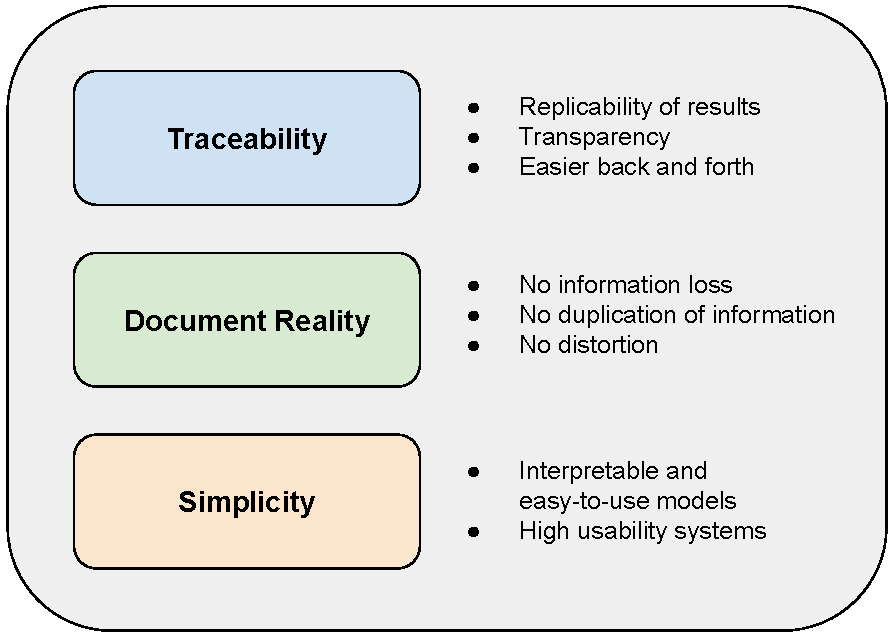
\includegraphics[width=0.70\linewidth]{static/figures/HSNAProcess/properties}
    \caption{Three properties essential to \va systems supporting the social historians workflow: \traceability, \reality, and \simplicity.}\label{fig:HSNA-properties}
\end{figure}
First, Traceable systems enable to do easier back and forth between the different annotation, modification, modeling, and analysis steps and provide a transparent chain of operations leading from the acquisition of the sources to the high-level socio-historical conclusions.
Traceability should be operated during the annotation and modeling process (for example to see why two mentions of persons have been given the same identifier, and to trace back network entities to the documents' annotations) but also during exploration.
Seeing every low-level operation (filter, selection, group-by, etc.) leading to the generation of insight leads to better transparency and replication\cite{callahanVisTrailsVisualizationMeets2006, xuSurveyAnalysisUser2020}.
Second, the digitization, encoding, modeling, and analysis/visualization steps should always reflect the textual reality of the documents \ie the \reality\footnote{We chose the term ``document reality'' over simply ``reality'' after a conversation with a historian to highlight the fact the historical documents do not describe factually the reality and reflect the subjective bias of the context in which the person wrote them\cite{karila-cohenNouvellesCuisinesHistoire2018}. The content of the documents, therefore, has to be modeled by taking into account this context, which can reveal interesting behaviors and structural patterns. See \cite{lemercierBackSourcesPracticing2021} for specific examples.}, in order to reduce the introduction of bias, simplification, and anachronisms in the analysis\cite{karila-cohenNouvellesCuisinesHistoire2018, lemercierQuantitativeMethodsHumanities2019}.
Indeed, encoding and modeling the data with abstraction and constructed concepts\footnote{In anthropology, the terms \emph{emics} and \emph{etics} refer respectively to intrinsic phenomena related to observation and constructed categories and abstractions\cite{headlandEmicsEticsInsider1990}.} such as the concept of families or ``social proximity'', often result in distortions (simplification or modifications), duplication, and loss of information contained in the documents.
Specifically, the choice of the network model embodies how the content of the sources is manipulated and abstracted with the goal of making historical conclusions, and deeply influences the annotation/encoding and analysis/visualization steps.
I discuss network models more in depth in the next \autoref{sec:modeling}.
Finally, as discussed in \autoref{sec:intro-HSNV}, social scientists often have trouble importing their data in \sna tools\cite{alkadi2022} and often perform ``soft SNA''\cite{rollingerProlegomenaProblemsPerspectives2020} only due to usability problems and ``Math anxiety''\cite{paxtonDollarsSenseConvincing2006}.
\va tools should therefore focus on \simplicity through the use of simple and comprehensible models and high usability systems.
The three properties and their effects on the workflow are summarized in \autoref{fig:HSNA-properties}.





\section{Network Modeling and Analysis}\label{sec:modeling}

% \subsection{Quantitative History}

% Traditionally, historians try to tell a story about protagonists and socio-economic facts in a given society. This narrative approach of history have been criticized for its lack of traceability and the open interpretation of historical documents, which can introduce bias from the author.
% Social history and HSNA brought answers to this problem by bringing quantitative methods to enforce a narrative supported by data and statistical results. However, traditional HSNA studies describe globally their sources without precising the annotation and transformation process they followed. They don't mention how the network they study has been obtained from the sources. Yet, these steps are critical as they can deeply influence the results of the analysis~\cite{lemercier_analyse_2005}~\cite{cristofoli_aux_2008}. Indeed, historians have to make choices on what to annotate and what to model into the network. This often depends on what they want to demonstrate at the end.
% As these steps of the workflow are often not transparent, it can be difficult for the reader of an HSNA study to understand how does the network has been constructed, what it represents, and to trace back the network entities from the original sources~\cite{dufournaud2018comment}~\cite{dufournaud_recherche_2015}.

% Recently, Experimental Computer Science went through a replicability crisis, pointing out that a lot of results were not reproducible, since authors were not giving enough data or information for people to redo the same analysis. Reproducibility is though considered a condition for building scientific knowledge, and this discussion highlighted the fragility of a lot of experimental studies. Data shows that the natural and social sciences are also affected~\cite{baker_1500_2016}.

% Usage of computer science in history can mitigate this problem, by providing methods and tools for historians to follow their analysis and providing traceability from their high level conclusions to the original documents.

% We argue one way of doing that is to use a network model which reflects well the \textbf{reality} of the social relationships mentioned in the documents, and are \textbf{traceable} to the original sources. We think network models which satisfy these two properties---\textbf{reality} and \textbf{traceability}---should always be constructed from the original sources as a basis for the analysis. Other network transformations can be applied afterwards to reveal specific patterns, but having a network which reflects well the reality of the documents is primordial for representing the sources as they are, and allowing to easily go back to them at any point in the analysis. Indeed, any transformation can be applied from a network representing well the sources. But applying modifications and transformations directly in the annotation process can bias the analysis and remove the possibility to follow other explorations and hypothesis in the future.

% Indeed, historians have to make choices on what to annotate and what to model into the network. This often depends on what they want to demonstrate at the end.
% As these steps of the workflow are often not transparent, it can be difficult for the reader of an HSNA study to understand how does the network has been constructed, what it represents, and to trace back the network entities from the original sources~\cite{dufournaud2018comment}~\cite{dufournaud_recherche_2015}.

% When transforming the information of the documents into a network, historians have to make choices on what to annotate and what to model into the network. As these steps of the workflow are often not transparent, it can be difficult for the reader of an HSNA study to understand how does the network has been constructed, what it represents, and to trace back the network entities from the original sources~\cite{dufournaudCommentRendreVisible2018}. Also, too complicated models are harder to visualize and analyze. For these reasons, we argue that a good network model should reflects well the reality of the social relationships mentioned in the documents, is traceable to the original sources, and is simple enough to visualize and understand.
% We think network models which satisfy these three properties---\textbf{reality},  \textbf{traceability} and \textbf{simplicity}---should always be constructed from the original sources as a basis for the analysis.

Historians typically construct one or several networks from their annotated documents that they visualize and analyze to validate or find new hypotheses.
As the processing steps of the workflow are often not transparent (digitization, annotation, network modeling), it can be difficult for the reader of an \hsna study to understand how the network has been constructed, what it represents, and to trace back the network entities to the original sources~\cite{dufournaudCommentRendreVisible2018}.
Moreover, visualizing the network very often highlights errors and artifacts of the annotations, along with potential mismatches between the network model and the analysis goals.
Historians then have to correct or change their annotations, even though it is a very tedious and demanding process to repeatedly switch back and forth between the network and the annotated documents.
Several network models make the task harder as they do not directly represent the documents, and it is thus difficult to relate a network entity to a specific document and annotation.
Therefore, I believe that more \va tools should support social scientists in annotating and modeling their documents to make the HSNA process less linear by allowing easier back and forth between the annotation, modeling, and visualization steps.
Network models satisfying  \traceability, \reality, and \simplicity properties would mitigate those problems by allowing to navigate more easily between the network and the documents while still modeling well the social relationships mentioned in the sources and being easy enough to visualize and manipulate for analytical and data modification goals.
%the data and detect potential errors and inconsistencies.

The choice of the network model to represent the social relationships mentioned in historical documents deeply influence the annotation and visualization/analysis processes.
Many network types have been proposed in the literature.
While simple ones---which are widely used---are easy to manipulate, they very often break \traceability---the network entities are not traceable to direct annotations, and sometimes correspond to constructed concepts---and the \emph{reality} of the documents.
On the contrary, complex models are often hard to manipulate and visualize.
I present the most widely used network models in the \hsna literature in \autoref{subsec:hsna-network-models} and present \modelplural as a model satisfying those three properties in \autoref{subsec:hsna-bipartite-model}.

\subsection{Network Models}\label{subsec:hsna-network-models}

Currently, historians use various network models depending on their knowledge of network science, the content of their documents, the schema of their annotations, and the analysis they plan to make. By ``model'' I refer to a mapping from the historical documents to a graph mathematical model and its semantic, \ie what the network entities represent in terms of sociological concepts (for example simple networks and co-occurrence networks have the same simple graph model $G = (V, E)$ but with different semantics).
I describe here the most used network models in \hsna along with more recent ones:

\begin{itemize}[nosep,leftmargin=*]
    \item \textbf{Simple networks~\cite{wetherellHistoricalSocialNetwork1998}:} According to their research hypotheses, historians select and merge document information to build a specific relationship between individuals. They analyze this simple network structure with \sna tools and produce network indicators and node-link visualizations. It is often difficult to connect the results to the original sources. Moreover, it does not take into account the diversity of social relationships, as every link is identical.
    \item \textbf{Co-occurrence networks~\cite{sairioMethodologicalPracticalAspects2009}:}
    % rubio-mondejarWomenEntrepreneursFamily2022}: % , keekMovementPerspectivesCollective, bouletBatchKernelSOM2008
    Only the persons are represented as nodes, and two persons are connected with a link when they are mentioned in the same document (or section). This can be a useful model to detect community-related patterns, but the constructed notion of ``proximity'' represented by the links simplifies and hide the diversity of social relationships.
    \item \textbf{Multiplex Unipartite Networks~\cite{eriksonMalfeasanceFoundationsGlobal2006}:} Only the persons are represented as nodes, and links model social ties between two persons. Links can have different types representing different types of social relationships. It allows the modeling of more complex social relations where people can have various social ties e.g. as parents, friends, and business relationships. However very often several possible representations for the same data exist as projections are often applied to the original documents to get this type of model.
    %, and very often several possible representations for the same data exist, especially for complex relationships. [jdf] true for the other network types
    \item \textbf{Bipartite/two-mode networks\footnote{Bipartite refers to the mathematical property that nodes of the network are split between two sets without any links between two nodes of the same sets, while the term two-mode refers to networks modeling two types of entities.}~\cite{hambergerScanningPatternsRelationship2014}
    %~\cite{hamberger_scanning_2014, lippPetitionsSocialContext2001a, shafie_hypergraph_2017}
    :} Nodes can have two types: persons and documents in this network model. A link refers to a mention of a person in a document and can thus only occur between a person and document nodes. Usually, links are not typed and only encode mentions.
    More recent analyses in \hsna encode the \emph{roles} of the persons in the documents as link types~\cite{Cristofoli2018}. This network model is more aligned with the original sources and allows following an analysis through the original documents themselves and not through concepts. It can also be used to represent constructed concepts, like the GEDCOM format which introduces the concept of ``family'' that ties together a husband, spouse, and children with different link types.
    The concept of family can have different meanings across time and cultures, meaning that GEDCOM adds a conceptual layer instead of grounding the network to concrete traceable documents and events (e.g., no marriage but birth certificates).
    % In our model, a family tie would be replaced by different documents: the marriage certificate and  birth certificates, to ground the network to concrete traceable documents and events.
    \item \textbf{Multilayer networks~\cite{multilayer}: } In these networks, each node (vertex) is associated with a \emph{layer} $l$ and becomes a pair $(v, l)$, allowing to connect vertices inside a layer or between layers. These advanced networks have received attention from sociologists~\cite{CRNOVRSANIN201456} and historians~\cite{vanVugt_2017}, but they are complex. The meaning of a layer varies from one application to another; it can be time (years), type of documents, the origin of sources, etc. They, therefore, offer many (too many) options for modeling a corpus, and visualizing it, with no generic system to support historians for taming their high complexity.
    \item \textbf{Knowledge graphs~\cite{hoganKnowledgeGraphs2021}: } they represent knowledge as triples $(S, P, O)$ where $S$ is a \emph{subject}, $P$ is a \emph{predicate}, and $O$ is an \emph{object}. Everything is encoded with these triples using controlled vocabularies of predicates and rules known as \emph{ontologies}. Knowledge Graphs are popular for encoding knowledge on the web, including historical knowledge. However, it is notoriously complex to encode documents using knowledge graphs due to the complexity of the format and the wide choice of possible ontologies. Most historians are unable to understand knowledge graphs and even less to use them for annotating a corpus. Since knowledge graphs are generic, they need complex transformations to be visualized, with no generic system to support historians in taming their high complexity.
\end{itemize}


%\autoref{fig:HSNA-network-models} shows a schematic representation of the different network models.
%We can rank the models given two axes: simplicity/complexity and specificity/expressiveness.
%Currently, historians mostly construct unipartite networks (simple, co-occurrence, and weighted) which are simple and allow them to answer specific questions.
%However, those models do not capture all the complexity of the documents and social scientists may miss important patterns.
%For example, modeling only co-occurrences of persons in documents remove the variety of social relationships these mentions can refer to~\cite{lemercier12FormalNetwork2015}.
%Several interpretations may coexist to explain why someone is central in the resulting network, which may be impossible to validate without encoding more information---such as the types of relationships---in the model.
%Depending on the schema of the annotations, it may be impossible to create more complicated networks at this step without redoing the annotation process which is costly in time and resources.
%On the contrary, too complicated models such as KG are difficult to create from the sources and are hard to visualize and analyze, especially for social scientists who are not trained in those kinds of formalisms.
%Using this kind of model usually requires learning complex query language to manipulate the data, such as the SPARQL language for KG\@.
%Therefore, we argue that historians should aim to model a network that is simple enough to manipulate, can be traced back to the original sources, and model well the social reality of the documents---i.e. having those three properties: \simplicity, \traceability, and \textit{reality}.

%We argue that historians should aim to model their networks simply enough to be manipulated by them, in a way that entities can be traced back to the sources, and expressive enough to model accurately the social reality of the documents---i.e., having those three properties:  \simplicity, \traceability, and \reality.

Currently, most digital history projects use one-mode networks (simple, co-occurrence, and multiplex) that are simple and allow answering specific questions, but they do not capture all the complexity of the documents, resulting in simplifications and distortions of the structural patterns.
I compare what would be the resulting networks for these models and the bipartite model of our three collaboration use cases (the example \dana is still in the phase of data acquisition), with additional information from the documents encoded as node and link attributes.
I do this for one given document for each dataset.
The results are shown in \autoref{tab:models}.

\begin{table}[!ht]
    \begin{tabular}{|m{4.5cm}|m{2.7cm}|m{2.7cm}|m{2.7cm}|}
        \hline Original Document & Co-occurrence            & Unipartite Multiplex    & Bipartite           \\
        \hline \tiny \underline{1712}: Construction of a church in \underline{Torino}.
        Associates: \colorbox{associate}{Bellotto G, Bello P.M, Bello G.}
        Guarantor: \colorbox{guarantor}{ Astrano G.A.}
        Approbator: \colorbox{approbator}{Corte A.} \linebreak
        \colorbox{associate}{Associate} \colorbox{guarantor}{Guarantor} \colorbox{approbator}{Approbator}
        & \centering\simplePiemont & \centering\unipartitePiemont & \bipartitePiemont   \\
        % \hline Le 7 octobre 1901, \colorbox{father}{François Marie Esnault} et \colorbox{mother}{Marie Julie Léopoldine Colson} ont déclaré la naissance de leur fille, nommée \colorbox{child}{Blanche Esnault} dans la commune de Saint-Maur-des-Fossés.uuu
        \hline \tiny Du \underline{dix-neuf fevrier mil huit cent quatre-vingt quatre}, à six heures du soir.
        Acte de naissance de \colorbox{child}{Dufournaud Alexis, enfant de sexe masculin} né le \underline{dix-neuf février}, à deux heures du soir au \underline{village de Grudet, commune de Saint} \underline{Symphorien}, des mariés \colorbox{father}{Dufournaud Alexis}, \colorbox{father}{cultivateur colon, âgé de trente ans}, et \colorbox{mother}{Marie Pardonnaud,} \colorbox{mother}{sans profession, agée de vingt-six ans}, demeurant au village de Grudet, dite commune de Saint-Symphorien. [...]
        \linebreak
        \colorbox{father}{Father} \colorbox{mother}{Mother} \colorbox{child}{Child}
        & \centering\birthSimple   & \centering\birthUnipartite   & \birthBipartite     \\
        \hline % \centering\includegraphics[scale=0.3]{OriginalPaperstatic/figures/HSNAProcess/OriginalPaperFigures/marriageDocumentnoParents}
        \tiny \underline{20-4-1659} : \colorbox{epoux}{\underline{Capitán} Alonso MUÑOZ de GADEA}, con Da. \colorbox{epouse}{Francisca CABRAL LEAL de AYALA}. Ts.: \colorbox{temoin}{Agustín Gayoso}, y \colorbox{temoin}{Juan Guerrero. Al margen: "\underline{fue Oficial Real}"}, (f. 9v). \linebreak
        \colorbox{epoux}{Husband} \colorbox{epouse}{Wife} \colorbox{temoin}{Witness}
        & \centering\simple        & \centering\noParents         & \bipartiteNoParents \\
        \hline
    \end{tabular}
    \caption{Resulting networks using different models produced by one document of the examples detailed in \autoref{subsec:hsna-examples}: co-occurrence, unipartite and bipartite models. The first column shows the partial transcription of real documents (simplification for collaboration \pascal). Colors represent annotations concerning the persons mentioned, their roles, and their attributes. Underlines refer to information related to the events and which can be encoded as document/event attributes.
    Only time is represented for simplification, but other attributes would follow the same schema.
    H: Husband, W: wife, T: Witness, M: Marriage, $A_N$: Associate, G: Guarantor, Ap: Approbator, C: Construction, F: Father, M: Mother, C: Child.
    }\label{tab:models}
\end{table}

As shown by Cristofoli~\cite{cristofoliAuxSourcesGrands2008}, we can clearly see the co-occurrence model removes the complexity of the social relationships and only show an abstract ``proximity'' between individuals.
Unipartite multiplex networks allow producing meaningful networks which model well the diversity of relations that can link several people.
It especially models simple relationships well, such as parenting ones as in example \nicole.
However, it produces distortions for more complex relationships involving more than two persons, as in example \pascal where people can either be mentioned as associates, guarantors, and approbators in the documents.
Associates should probably be linked together with \textit{associate} links, but the \textit{guarantors} and \textit{approbators} relationships are more complex to model.
Approbators could be linked to the associates, the guarantors, or both.
The three ways of modeling this type of relationship make sense but can lead to very different network shapes and analysis results.
Historians thus have to decide on a transformation among several possibilities, which will probably distort the social reality of the relationships.

These examples also show that when working with multivariate networks, using projections to create unipartite networks brings a duplication of information.
Indeed, if a document mentions information like a date that we model as an attribute, we can store it as a document node attribute using a bipartite model.
However, when projecting the network, this information appears in the links as many times as there are persons mentioned in the document minus one and often more.
For example, in the example \pascal in \autoref{tab:models}, the time of the construction is stored in $\sum_{i=1} ^{4} i = 10$ links in the co-occurrence model and in 9 links in the multiplex unipartite model, while it is only stored once as a document node attribute in the bipartite model.

Both co-occurrence and unipartite multiplex models thus do not satisfy the \reality property by introducing constructed concepts---such as abstract notions of ``proximity''---or inferring one-to-one social relationships from mentions in a document mentioning more than two actors.
Moreover, projections add ambiguity in retrospect of the original documents, as it becomes impossible to trace back one link to one specific document, as the same link could potentially refer to several ones~\cite{cristofoliAuxSourcesGrands2008}, \ie they do not satisfy the \traceability principle.

More complex models, such as multilayer networks and knowledge graphs, could satisfy \reality and \traceability principles (depending on the modeling choices, as these models are very expressive and do not enforce specific data schemas) but are complex to manipulate and visualize, especially for social scientists.
In contrast, the bipartite model satisfies the \reality and \traceability properties through the representation of documents as nodes, and individuals' mentions as links encoding their roles.
This model is simple enough to manipulate according to the number of \sna studies leveraging it \cite{lippPetitionsSocialContext2001, shafieHypergraphRepresentationsStudy2017, davisDeepSouthSocial2009, ochabDetectingOttokarII2022} and the development of \sna bipartite measures and algorithms\cite{borgattiSocialNetworkAnalysis2009, latapyBasicNotionsAnalysis2008, hambergerScanningPatternsRelationship2014}.
Yet, most \hsna studies are based on the network topology and often do not leverage attributes, including time and location.
We, therefore, claim that \modelplural allow to model historical documents with \traceability, \reality, and \simplicity properties.
I formalize and describe this model in the next \autoref{subsec:hsna-bipartite-model}.

%For example, modeling only co-occurrences of persons in documents remove the variety of social relationships these mentions can refer to\cite{lemercier12FormalNetwork2015}.
%Moreover, since documents are not explicit in the unipartite model, it is hard to trace the network entities back to the sources: the traceability property is not satisfied, meaning that the data is harder to correct and that analyses are less replicable.
%On the other side, multilayer networks and knowledge graphs allow to model documents as entities and express complex relationships between various other entities they mention.
%These models can be very expressive but are challenging to use for historians, especially without guidelines; without \simplicity, the \traceability and \reality properties can be hard to achieve.
%The lack of simplicity, therefore, results in difficulties for visualization and analysis, especially for social scientists.


% TODO: maybe to a better figure
%\begin{figure}
%    \centering
%    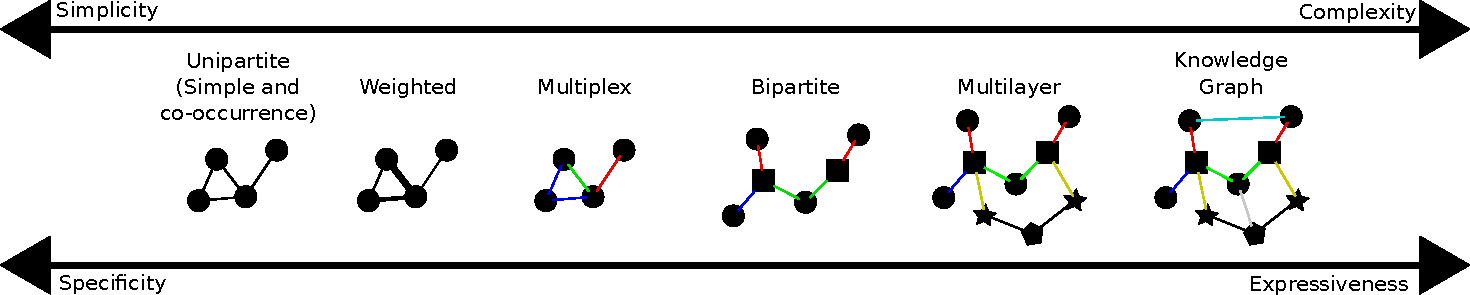
\includegraphics[width=\columnwidth]{static/figures/HSNAProcess/OriginalPaperFigures/models.pdf}
%    \caption{Schematic representations of Different network models used for analyzing historical documents, ordered by complexity and expressiveness}
%    \label{fig:HSNA-network-models}
%\end{figure}

%\autoref{fig:HSNA-network-models} shows a schematic representation of the different network models, ranked on simplicity/complexity and specificity/expressiveness axis.


% \begin{table}
% \centering
% \resizebox{\columnwidth}{!}{%
% \tiny
% \begin{tabular}{|l|l|l|l|}
% \hline
%                               & Traceability & Reality & Simplicity \\ \hline
% Simple Networks               & \xmark       & \xmark  & high       \\ \hline
% Co-occurrence Networks        & \xmark       & \xmark  & high       \\ \hline
% Multiplex Unipartite Networks & \xmark       & \xmark  & high       \\ \hline
% Bipartite Networks            & \cmark       & \cmark  & medium     \\ \hline
% Multilayer Networks           & \cmark       & \cmark  & low       \\ \hline
% Knowledge Graphs              & \cmark       & \cmark  & low  \\ \hline
% \end{tabular}%
% } \caption{Network models table.}
%  \label{tab:HSNA-modelsAndProps}
% \end{table}

\subsection{Bipartite Multivariate Dynamic Social Network}\label{subsec:hsna-bipartite-model}

Historical documents are well modeled by bipartite multivariate dynamic networks with roles, that can be formalized as

\begin{equation}
    G = (V, E, B, R, T, L)
\end{equation}

where $V$ is the set of vertices, $E$ the set of edges, and $B = (person, document)$ the set of node types.
Each node $u \in V$ is defined as

\begin{equation}
    u = (u_{id}, b_u, a_u)
\end{equation}

where $u_{id}$ corresponds to the unique identifier of $u$, $b_u \in B$ is the type of the node and $a_u$ is a tuple of the attributes (or properties) values of $u$. If $b_u = person$, then

\begin{equation}
    a_u = (a_i, \dotsc, a_N)
\end{equation}

with $a_i, \dotsc, a_N$ the attributes values of the node $u$ of the $N$ attributes defined on person nodes, defined on their domains $A_i, \dotsc, A_n$.
Document nodes always have a time and location such that for a document node $v \in V$  with $b_v = document$ then

\begin{equation}
    a_v = (t, l, a_i, \dotsc, a_M)
\end{equation}

with $t \in T$ is the time of the event witnessed by the document, $l \in L$ its location, and $a_i, \dotsc, a_M$ the attributes values of the node $v$ of the $M$ attributes defined on document nodes (other than time and location), defined on their domains $A_i, \dotsc, A_M$.
Similarly, each edge $e \in E$ is defined as

\begin{equation}
    e = (u, v, r, a_e)
\end{equation}

with $u, v$ the vertices connected by $e$ such that $b_u \neq b_v$, $r \in R$ the role of the person mentioned in the document and $a_e$ the attributes tuple of $e$ such that

\begin{equation}
    a_e = (a_i, \dotsc, a_O)
\end{equation}

with $a_i, \dotsc, a_O$ the attributes values of the edge $e$ of the $O$ edge attributes defined on their domains $A_i, \dotsc, A_O$.

The model has, therefore, the following properties:
\begin{description}[nosep,leftmargin=2mm]
    \item[{Bipartite:}] There are \textbf{two types of nodes}, persons and documents (or events). An event, such as a marriage, is most of the time witnessed by a document, and we refer to them interchangeably as events and documents. Events considered in the network can be of the same sub-type, such as contracts, or of multiple subtypes, \eg for genealogy: \emph{birth certificates}, \emph{death certificates}.
    \item[Links and Roles:] A link models the mention of a person in a document. \textbf{Each link has a type corresponding to the role of the person in the document}. For a marriage act, the roles include \emph{wife}, \emph{husband}, and \emph{witness}. This is a key aspect of our model since it clarifies the relationship between the persons within an event. In contrast, Jigsaw~\cite{staskoJigsawSupportingInvestigative2008} does not consider the roles.
    \item[{Multivariate:}] Each entity of the model can have attributes, that give additional information. Person nodes are referenced by a key that reflects the disambiguation process. They can have general information (standardized name, gender, birth date). Documents are also identified by a key, \eg an archive reference. The associated event can have a date, a location, and potentially other information. Links can also carry information to describe contextual properties (activity, residence, etc.).
    \item[{Geolocated:}] Events should have a location when it makes sense, ideally with the longitude and latitude.
    \item[{Dynamic:}] Events are always dated. We rely on this date since it encodes the social dynamics of the network.
\end{description}

One of the main benefits of this model is that the document nodes represent both the physical documents and the events the documents refer to.
For example, concerning marriage acts, the document nodes represent both the physical documents with their texts but also the marriage events with their characteristics modeled as attributes (time, location, etc.).
Therefore, social historians can use this model to store, process, and annotate their original documents and follow an analytical workflow with the same representation.
This model is \textit{simple} enough to manipulate and visualize for historians and allows tracing back every entity of the network to the documents according to the \traceability principle.
Still, the network preserves the \reality of the social relationships mentioned in the sources as no projection or transformation is applied.

Visualization tools using this model can focus on the topology of the network, and/or the attributes which I express here in the format of tuples, commonly used by databases and visualization systems\cite{stoltePolarisSystemQuery2002}.
However, it has to be taken into account that if the attributes extracted from the historical documents are related to vertices and edges independently to the topology of the network, it can be appropriate to compute vertices and edges measures---such as the centrality---and store them similarly to the other attributes, especially so that visualization systems can leverage the same interactions for both.
In that case, these types of attributes are directly dependent on potential topology changes in the network (for example after subgraph extraction or network modification interactions).


\section{Applications}\label{sec:hsna-applications}

%% After constructing their network, historians can explore and analyze them using specifically designed visual analytics tools.
%Several tools have been designed for visualizing dynamic bipartite networks that can also be considered dynamic hypergraphs~\cite{valdivia_analyzing_2021, penaarayaHyperStorylinesInteractivelyUntangling2022}, but few incorporate attributes and complex interactions.
%We designed ComBiNet~\cite{pister2022visual} to explore and navigate through historical documents modeled as \modelplural and to help social scientists answer their questions with the help of visual queries and interactive comparisons of query results. \autoref{fig:HSNA-combinet} shows the interface to compare two meaningful groups of construction documents in Piemont during the 18th-century~\cite{Cristofoli2018}. In this example, we see that the \textit{Zo} family has more construction contracts in \textit{Turin} than the \textit{Menafoglio} family.
%Exploring historic datasets modeled as \modelplural allows answering complicated questions both related to the events (here the constructions) and the persons while being able to trace back to the original documents directly in the interface for cleaning or debugging purposes.
%% Exploring historic datasets modeled as \modelplural allows answering complicated questions both related o the events (here the constructions) and the persons while being able to trace back to the original documents directly in the interface for cleaning purposes.


Several tools have been designed for visualizing dynamic bipartite networks that can also be considered dynamic hypergraphs~\cite{valdiviaAnalyzingDynamicHypergraphs2021, hyperstorylines}, but few incorporate attributes.
Moreover, the vast majority of visual analytics tools are solely focused on the analytical part of the data, meaning that the link between the original documents and the hypergraph abstraction is often broken.
Social scientists, therefore, always have to do many back and forth between the visual analytics tools and their original documents and the annotation/modeling processes.
More visual analytical tools should thus incorporate the textual documents in their data model similarly to Jigsaw\cite{staskoJigsawSupportingInvestigative2008}, as it would allow tracing the entities of the network back to the original documents more easily.
Mechanisms to modify the annotations and reflects on the network modeling process directly in the analytical environment could also ease the social scientists' workflow loop.
It would allow them to directly correct errors and inconsistencies in the annotations and propagate them in the visual analysis workflow.
I propose in \autoref{ch:combinet} and \autoref{ch:pk-clustering} two proof-of-concept interfaces leveraging \modelplural as a representation of social historians sources with the aim of analysis, network modeling, and reflection on the encoding process, with a focus on \traceability, \reality, and \simplicity.
%For example, the Vistorian\cite{serranomolineroUnderstandingUseVistorian2017} lets users modify and correct their data in a table format if they see errors or inconsistencies.


\section{Discussion}

% We propose a way of modeling the majority of historical document datasets using \modelplural, as it satisfy \textit{reality}, \traceability and \simplicity properties in relation to the original documents.
% We also argue for the elaboration of visual analytics tools to explore and analyze this type of data. However, other network models could be better suited for answering some questions or to represent specific underlying phenomena. Simple network models such as co-occurrence networks can be effective to answer simple questions related to the centrality for example, while more complex models such as multipartite networks could also be used to model more complex entities.
% However, we think using \modelplural as a first step in the analysis is a good way of stepping in the network domain space while keeping the traceability to the original sources, and can be used easily to create other networks with the help of projections and transformations~\cite{andrei2011porgy}.

Most tools for social network visualization focus solely on the visualization and analysis steps, without considering the whole historical data analysis process, preventing researchers from going back to the original source, and supporting the social analyst in the annotation and modeling steps.
I think visual analytics tools helping social scientists annotate and model their data with \reality, \traceability, and \simplicity principles in mind are essential to conducting socio-historical inquiries with limited friction, realistic training, and scientific transparency.
% useful if even more than purely analytical systems and can be an interesting research direction.
Concerning the network modeling step, \modelplural model well the majority of structured historical documents such as marriage acts, birth certificates, and business contracts as these documents refer to specific events (birth, marriage, transaction, etc.).
The two-mode structure enables the representation of both the persons and the documents/events, without any simplification or distortion of the social reality of the documents and their annotations, compared to the classical one-mode representation\footnote{Another approach proposed by Everett and Borgatti is to have a dual-projection of this two-mode network to manipulate simultaneously two linked one-mode networks\cite{everettDualprojectionApproachTwomode2013} (in our case person-person and document-document). The Detangler visualization system successfully proposed such an approach\cite{renoustDetanglerVisualAnalytics2015}.}.
The document nodes represent both the textual documents and the specific events.
This dual representation works well for semi-structured documents but could be more limiting for other more literary documents.
Moreover, structured documents can also provide information about other relationships not directly linked to the main event.
For example, marriage acts sometimes refer to the place and date of birth of the spouses with the names of the parents.
This information relates to the birth of the spouses and not the marriage specifically.
In that case, social historians can either ignore this type of information in the annotation process or encode it with specific roles ( for example \textit{husband's father} and \textit{wife's father}), thus turning the network into a model of the documents only, and not events.
We show what would look like the resulting networks \autoref{fig:HSNA-doc-vs-event-model}for the two cases where marriage acts mention birth information and the case where only marriage-related information is present in the document.

\begin{figure}
    \begin{overpic}[width=\linewidth, trim={0 0 0 0},clip]{static/figures/HSNAProcess/documentVsEvents.pdf}
        \put(4,7){\bipartiteParentsOneEvent{1}}
        \put(42,10){\bipartiteNoParents}
        \put(70,7){\bipartiteParents{1}}
    \end{overpic}
    \caption{bipartite multivariate dynamic network modeling for two cases of marriage acts of example \zacarias. Some marriage acts mention the parents of the spouses, which is a relationship different than the marriage in itself. This case can be modeled using a document model (a) or an event model (c) by splitting the document into several different event nodes. The other case refers to documents that do not mention the parents (b), and in that case, the network represents both the documents and the events with the same model. M: Marriage, H: Husband, W: Wife, T: Witness, (H/W)(M/F): Husband/Wife Mother/Father. Yellow links refer to parenting mentions/relationships.}\label{fig:HSNA-doc-vs-event-model}
\end{figure}

%\bipartiteParentsOneEvent{1}
%\bipartiteNoParents
%\bipartiteParents{1}

% Concerning, the \model model, it represents well the majority of historical documents such as marriage acts, birth certificate and business contracts as these documents refer to specific events (birth, marriage, transaction etc). The document nodes therefore represent both the textual documents and the specific events. The person nodes linked to the documents nodes represent then both a mention in the document but also the participation of this person in the event (the role being modeled as link type). This dual modeling works well for this type of structured documents but could be more limiting for other types such as conversational letters.
% Moreover, structured documents can also provide information about other relationships not directly linked to the main event. For example, marriage acts sometimes refer to the place and date of birth of the spouses with the names of the parents.
% In that case, social historians can either ignore this type of information in the annotation process or still encode it. In the latter, the network will reflect the documents but not the events.

% Several projections


\section{Conclusion}

\hsna is a complex process that starts by collecting historical documents and ends with elaborating high-level sociological conclusions.
Historians support their conclusions by modeling individuals' social relationships extracted from the documents and analyzing them through network visualization and analysis methods.
Most historical work do not provide details on how they constructed their final network, even though it is a complicated and tedious process that can result in many biases and distortions if not done carefully\cite{alkadi2022}.
We shed light on this process by dividing it into 5 steps and describing recurrent pitfalls we encountered in our projects and collaborations.
More importantly, I explain why this process should be done following the principles of \traceability, \reality, and \simplicity to avoid biasing the analysis, allowing to go back to the original source at any point of the workflow for easier corrections and replicability, and using models and methods simple and powerful enough for social scientists.
Visual analytics software designed for \hsna should consider those principles to provide tools allowing to follow non-biased and reproducible analysis starting from the raw documents while supporting historians in going back and forth more easily between the annotation and analysis/visualization steps.
I discussed the network modeling process in depth and claimed that \modelplural satisfy those three core principles, letting historians both wrangle their data and characterize sociological phenomena using a common model and visual representation, thus answering \qone.
Using this model, \va interfaces could help social scientists manage and analyze their data, starting at the data acquisition and annotations steps instead of focusing on the analysis only while providing efficient representations of the data for analysis and exploration.
We explore what could be such VA interfaces in the next two chapters.

    \chapter{ComBiNet: Visual Query and Comparison of Bipartite Dynamic Multivariate Networks with Roles}\label{ch:combinet}

In the previous chapter \autoref{ch:hsna-process-and-network-modeling}, we showed that \modelplural allow to model well historical documents, with \emph{simplicity}, \emph{reality} and \emph{traceability} properties.
However, no visual tools currently exist to explore and analyze this type of data.
In this chapter, we propose a \va interface aimed at exploring historical documents modeled as \modelplural.
We try to answer \textbf{Q2} by analyzing tasks and questions historians have on their data and providing interactions mechanisms which would allow them to answer their historical questions while finding errors in their data.

\paperbox{This chapter is an updated version of an article currently submited to the journal Computer Graphics Forum, and a poster presented at the conference EuroVis 2022 \cite{pisterVisualQueriesBipartite2022}. It was a joint work with my advisors Christophe Prieur and Jean-Daniel Fekete. I did the development of the interface, and led in the discussions, evaluation, and writing of the paper.}


\section{Context}

Social scientists such as historians aim at characterising the structure and dynamics of social groups of interest, on a region and period of time they focus on\cite{tilly1984retrieving}.
Their work essentially relies on documents---such as marriage acts, census records, surveys, and business contracts---to gather information about the life of important actors that they explore in-depth, or to draw conclusions on social aspects of groups in the society of that period and place.
Instead of drawing conclusions from their gathered knowledge and interpretations of the documents, a more systematic approach consists in constructing a social network from the documents and following a network analysis approach~\cite{wetherellHistoricalSocialNetwork1998}.
For this, they need to encode their documents to extract the persons and any other useful information in the text and transfer it into a structured file or a database.
Social scientists can then explore, validate, or refute their hypotheses by visualizing and analyzing the network structure and the connectivity patterns between the entities of the resulting network.

Currently, social scientists often model their datasets as simple networks where the nodes are the persons mentioned in the documents (see \autoref{ch:hsna-process-and-network-modeling}).
Usually, Two persons are then connected together in the network when they appear in shared documents.
This representation is easy to visualize and analyze but simplifies and distorts the information by hiding the documents that witness the relationships between the persons.
Thus, another approach consists in modeling the data as bipartite networks, where both the documents and the persons are represented as nodes and are connected together when a document mentions a given person~\cite{grandjeanAnalisiVisualizzazioniReti2017, rossiExplorationLargeDatabase2014, shafieHypergraphRepresentationsStudy2017}.

In addition, historical documents include time and geospatial information corresponding to the date and location of the events they refer to, and potential additional information on the mentioned individuals such as their gender, profession, and date of birth.
These are often essential to understanding underlying social phenomena, as time, space, and classical social categories play an important role in sociological structures and dynamics\cite{lemercier12FormalNetwork2015}.
For these reasons, as we discussed in \autoref{ch:hsna-process-and-network-modeling}, historical sources and the underlying social events they refer to can be modeled well by \emph{bipartite} with \emph{roles},  \emph{multivariate} \emph{dynamic} networks. \emph{Bipartite} means that both persons and documents (or events, that are often witnessed by physical documents) are modeled as typed nodes. \emph{Multivariate} means that the nodes and links can carry additional attributes. \emph{Dynamic} means that time is a mandatory attribute of documents.
Furthermore, a link created between a person's node and a document's node (when the person is mentioned in the document), has an associated link type that models the \emph{role} of the person in the document/event.
Additionally, documents can optionally carry a geographical location.
This model unifies several social network models and allows to represent historical documents with simplicity, traceability, and document reality, \ie the relationships appear as they are mentioned in the documents without distortions implied by projections\cite{cristofoliAuxSourcesGrands2008}.

More complicated models exist such as knowledge graphs\cite{opitzInductionLargeScaleKnowledge2018}, which are very expressive but hard to manipulate, especially for social scientists.
In contrast, most visual and analytics tools widely used by social scientists such as Gephi~\cite{Gephi} and NodeXL~\cite{NodeXL} enforce too simplistic network models and only provide limited interactions for exploring the network data, even if they provide the computation of several network measure.
This results in many social historians end their analysis by plotting the network using a node-link diagram---which is hard to read with dense networks---, and identifying the most important actors with the help of centrality measures\cite{lemercierQuantitativeMethodsHumanities2019}.
Lemercier \& al complain about this phenomenon: ``Network graphs of the “spaghetti monster” variety are a case in point. Often, in historical papers, they are used to show that a network is dense (and that the author has mastered the new technology). The narrative then comments on the individuals identified as central in the network. This approach can indeed be quite interesting, but it is hardly the only possible use for network analysis.\cite{lemercierQuantitativeMethodsHumanities2019}''.

\va tools guiding social scientists towards more complex exploration with the help of interaction mechanisms are therefore needed.
% Contrary to the early taxonomy of tasks on graphs~\cite{lee:hal-00851754}, with the data model we use, it becomes impossible to characterize a finite set of simple tasks to support, along with their associated visual representations and interactions techniques.

In this chapter, we present a visual analytic system to explore and analyze Bipartite Multivariate Dynamic Social Networks, with the aim of answering historical and sociological questions.
We elaborated our tool based on four collaborations with social scientist colleagues.
We first collected important questions they each had on their data and transcribed them from a network analysis perspective.
The majority of the questions raised consisted in either finding specific patterns in the network---corresponding to specific groups or individual exhibiting intriguing behaviours---or in comparing several subsets of the network, in terms of network measures, attribute distributions, and their overlaps.

% In this paper, we thus present a visual analytic system to explore and analyze Bipartite Multivariate Dynamic Social Networks. Based on the needs and questions of our collaborators,
we thus focus on three high-level tasks: exploration, queries, and comparison of this type of network.
Users can explore the data using two layouts: a node-link bipartite view showing the sociological structure of the network, and a map layout based on the geolocation of documents.
We designed and implemented a new visual graph query system that allows us to build both topological and attribute constraints, based respectively on a node-link interactive representation, and dynamic widgets.
For this, we rely on the Neo4j graph database~\cite{neo4j} and its language \emph{Cypher}.
Most visualization systems offer dynamic queries to hide the complexity of query languages.
However, using a rich data model, some queries are easier to refine using scripting than dynamic queries.
We implemented dynamic queries that also show the translated Cypher queries, and inversely, can translate textual queries into visual queries.
With that interface, social scientists can start building their queries with simple widgets and, if needed, complement them by editing the query, alone or with the help of power users.
Furthermore, they can export their query, the associated results, and its history at any point to share it with someone else or to start an analysis session from a previous result.
\name also implements subgraph comparison techniques, allowing the comparison of networks, network-related measures, and attribute distributions between the entities returned by the queries.
% In this first version of \name, we focused on the power of queries and comparisons and not usability so most of the explorations have been done by one of the authors or close to.
We validate the query and comparison system with a formative usability study and we demonstrate \name can be used to answer sociological questions by describing in depth several real-world use cases.

% 1) a succession of attribute and topological queries that are usually applied sequentially, from the simplest to the more complex, % which can be done with a graph database system and associated query language;
% \item The comparison of several query resulting subgraphs, in terms of connectivity metrics or attribute distributions
% and 2) the comparison of networks, measures, and attribute distributions, either between the entire network and the results of a query or between two separate query results.
% Several sophisticated tools exist to explore and analyze rich social networks, such as Gephi~\cite{Gephi}, NodeXL~\cite{NodeXL}, Jigsaw~\cite{Jigsaw}, or VERTIGo~\cite{cuenca_vertigo_2021}. However, these tools often enforce a data model which are often either too simple
% except for Jigsaw, they provide too limited interactions to query and explore richly encoded data.

% Social Science use node link diagram
% There are now bipartite approaches
% Historical sources use time, attributes, locations. there should be more of these
% Need tools to explore these specific kind of dataset
% Query and comparison to answer historical and sociological questions

After the related work section, we describe our design process in \autoref{sec:combinet-tasks}, present our system \name in \autoref{sec:combinet-system} with the design of the visual query and comparison features, and present three use cases demonstrating the utility of our system in \autoref{sec:combinet-usecases} showing it can be used to explore complex historical data and allowing historians to answer several of their questions using queries and comparisons.
We finish if the results of the formative usability study in \autoref{sec:combinet-usability}.
Our contributions are:
\begin{itemize}
% \item The description, motivations, and benefits of our unified data model: \emph{bipartite} with \emph{roles}, \emph{multivariate} and \emph{dynamic}, for the visual exploration and analysis of social networks;
% \item The design and implementation of a bipartite graph visualization and map layout specific to social scientist needs.
    \item The design and implementation of a graph query system, synchronizing the visual representation of the query and the associated script;
    \item The design and implementation of visualization and interaction techniques aimed at comparing subgraphs, in terms of topology, attributes, time, and geographical location.
    \item A usability study and three real-world use cases demonstrate the utility of the system to answer socio-historical questions.
\end{itemize}



\section{Related Work}\label{sec:combinet:related-work}

As we already discussed the related work on network modeling and social network visualization in \autoref{ch:related-work} we only discuss in this section the related work on graphlet analysis, visual graph querying, visual graph comparison, and provenance.

\subsection{Graphlet Analysis}

One of the inspirations for this project came after participating in the 2020 VAST challenge\footnote{This is a challenge organized in the context of the IEEE Visual Analytics Science and Technology (VAST) conference. The challenge consisted of a series of analytical questions united under an overarching cyber threat scenario. We participated in the Mini-Challenge 1 which asked participants to identify a group of people that accidentally caused an internet outage. To identify this group, we were given a network profile and a large multi-variate social network to search in.} where our team used graphlets to measure similarity between several networks~\cite{tovanichVAST2020Contest2021}.

Graphlets are small connected induced, non-isomorphic subgraphs composing any network (see \autoref{subsec:methods-and-measures} for mor details).
They were first introduced by Milo et al.~\cite{miloNetworkMotifsSimple2002} to explore the structural differences between biological networks, but they are now used in several disciplines involving networks such as sociology\cite{charbeyStarsHolesPaths2019}.

One of the aims of the VAST 2020 challenge was to compare several multivariate networks.
However, by using graphlets we realized that 1) it was not very efficient to compare several networks in contrast to other measures and 2) the interpretation of all graphlets patterns that are found in a network is complicated given the fact that one specific pattern can have various interpretations given the nodes involved and their positions in the network~\cite{ingramNetworkMotifsStructure2006}.
This is especially true that the number of potential graphlets grows exponentially as we increase the number of nodes considered (there are 6 graphlets of size 4 and 21 graphlets of size 5 for example) and if we add complexity to the network model, for example by using directed links or node and link types~\cite{ribeiroDiscoveringColoredNetwork2014}.

Instead of counting every graphlet occurrence and interpreting them with sociological meanings, it appeared more efficient to let social scientists finding specific patterns to answer questions they ask themselves on the data.



\subsection{Visual Graph Querying}


% Guess~\cite{adar_guess_2006} has been designed to provide a dual view of networks, one from a scripting language (a variation of Python) coupled with a visual representation of the network. However, it still relies on scripting to search and manipulate the network, contrary to modern visualization systems using dynamic queries~\cite{DynamicQueries}.

Graph pattern matching is an important task in \sna, which consists in finding a subgraph of interest in a larger graph\cite{fanGraphPatternMatching2012}.

Several scripting languages, such as R~\cite{Rstat} and Python~\cite{Python}, have been extended to support the exploration of social networks using specialized libraries such as igraph~\cite{igraph} and NetworkX~\cite{NetworkX}, and provide functions for graph pattern matching.
However, social scientists are often challenged to use scripting languages and programming, as they often do not have formal training in such technologies.

Graph databases allow to store and manipulate network data with the use of query languages, such as the Cypher language for Neo4j\cite{neo4j}.
%Constructing and querying a pattern from a graph requires knowledge of graph databases and query languages.
To lower the complexity barrier of their usage, several visual graph query systems have been developed to allow analysts to rapidly build and refine their queries visually.
Some systems hide the scripting language such as GRAPHITE~\cite{chauGRAPHITEVisualQuery2008} and VERTIGo~\cite{cuencaVERTIGoVisualPlatform2021} that allow specifying a graph query as a node-link diagram that the user creates interactively.
Shadoan and Weaver~\cite{shadoanVisualAnalysisHigherOrder2013} use a similar concept with hypergraphs to filter multidimensional data.
Other systems, such as VIGOR~\cite{pientaVIGORInteractiveVisual2018} only visualize the query after it has been written by the user with a scripting language and do not allow direct interaction of the visual representation of the query.
All these visual query systems are limited to topological queries with constraints on the vertex and edge types and do not allow to make constraints on other dimensions such as attributes and time associated with vertices and edges.

\iffalse
\subsection{Tasks Taxonomies}

Lee et al.~\cite{lee:hal-00851754} have introduced a taxonomy of tasks related to general graphs.
It relies on the taxonomy of low-level activities by Amar et al.~\cite{Amar05}, and extends it by considering different types of tasks: topology-based, attribute-based, browsing, and overview. These tasks can be applied to different kinds of graph-specific objects: nodes, links, paths, and various kinds of groups.
They also mention higher-level tasks but not time.

This taxonomy has been extended for dynamic networks by Bach et al.~\cite{bach:hal-00906597} and Ahn et al.~\cite{Ahn14}, using a similar method of applying the low-level taxonomy of Amar et al.\ to all the graph objects plus time. The method reaches its limit here since the number of tasks is proportional to the Cartesian product of the objects considered and time, and becomes too large to be fully discussed.
In parallel, Adrienko \& Andrienko~\cite{andrienko2006exploratory}
Kerracher et al.~\cite{Kerracher15} summarize these taxonomies \jdf{Revise the Andrienko' taxonomy for our bipartite networks.}

None of these taxonomies mention ``comparison'' as a primary task, maybe because, in their reference taxonomy of interaction techniques, Yi et al.~\cite{yiDeeperUnderstandingRole2007} write: ``we debated adding a \emph{Compare} category but ultimately
omitted it because we believe that Compare is a higher-level user goal or objective than the other user intents we identify''. Gleicher~\cite{Gleicher18, gleicherVisualComparisonInformation2011} develops an abstract framework to clarify the ``comparison'' task in visualization and argues for its importance.
We agree with Gleicher since several of the use cases reported by our social scientists' colleagues involve comparisons.
\fi

%\vspace{-2mm}
\subsection{Visual Graph Comparison}

Gleicher et al.~\cite{Gleicher18} propose a taxonomy of visual comparison designs for complex objects. They claim any visual comparison system can be classified into one (or a mix) of the three following categories: juxtaposition, superposition, or explicit design.
Yet, few visual systems support comparison tasks for social networks.

Andrews et al.~\cite{andrewsVisualGraphComparison2009} describe a technique to compare several networks, using a combination of juxtaposition and superposition techniques.
The two candidate networks are shown side by side, along with a third view composed of a fusion network highlighting both the shared nodes along with the non-shared nodes with different colors.
%
Freire et al~\cite{ManyNets} describe the ManyNets system to compare many networks by using a table where each describes one graph and each column shows graph measures in terms of small visualizations, from simple bars to distributions, allowing the comparison of a large number of graphs. However, ManyNets does not visualize the networks per se (no layout shown), and do not take into account attributes, node types, or time.
%
Hascoët and Dragicevic~\cite{HascoetD12} describe a system to match and compare graphs using superposition, focusing on the topology, not taking into account attributes or time.
Tovanich et al.\cite{tovanichVAST2020Contest2021} propose a visual analytics tool to compare multivariate, sometimes bipartite, dynamic networks and find common structures.
However, their tool does not handle roles and is designed for the specific task of matching a subgraph into a larger network.

\subsection{Provenance}

Provenance in the context of Visual Analytics consists in the logging of the sequence of actions of users on an interactive visualization system during analysis sessions.
Collecting provenance information has proven to benefit users by providing them action recovery (undo) plus collaborative and reproducibility capabilities~\cite{raganCharacterizingProvenanceVisualization2016}.
For example, the VisTrails system allows users to reproduce their visual analyses by providing an executable history graph of their actions,~\cite{callahanVisTrailsVisualizationMeets2006} while GraphTrail provides provenance tools to ease collaborative analysis~\cite{dunneGraphTrailAnalyzingLarge2012}.
Provenance can also be beneficial for visualization designers and researchers, as it gives them a tool to understand users' behaviors~\cite{battleCharacterizingExploratoryVisual2019, borsProvenanceTaskAbstraction2019}
and evaluate/improve visualization systems~\cite{renCharticulatorInteractiveConstruction2019}.
All the reasons and concrete implementations of provenance are discussed in depth in Xu's survey~\cite{xuSurveyAnalysisUser2020}.

\section{Task Analysis and Design Process}\label{sec:combinet-tasks}

I designed the \name tool in collaboration with social historians who wanted to follow a network analysis on their historical semi-structured documents, that are well modeled by \modelplural.
I first collected questions they had about their data and what they wanted to see in a visual interface.
By analyzing the questions we leveraged tasks and requirements that I used to design and implement the interface, with continuous feedback from our collaborators.
%We designed the interface from the requirements with continuous discussions with our collaborators.
%We showed them visual prototypes during the development phase to get feedback iteratively.

\subsection{Use Cases}

We elaborated this interface from the collaborations with historians we described in \autoref{sec:HSNA-examples}.
These collaborations involved regular meetings and multiple discussions over two years.
All these datasets are textual corpora constituted of historical documents mentioning people with complex relationships, which are well modeled with \modelplural.
We give more details about the datasets of these collaborations in this section, along our collaborators' main questions with the associated network queries to answer them.
The full answers involve visualizations of the query results and attribute summaries that I describe in the next section.
%We list the most important questions our collaborators shared with us on their respective datasets.
We categorized the questions according to four dimensions: global (G)/local (L) (do they want to categorize a group of nodes or retrieve specific persons/documents), if the question can be answered using the topology (T), and/or the attributes (A), and finally if a comparison (C) using several filters is needed or not (N).

\begin{enumerate}
    \item Analysis of the social dynamics from \textbf{construction contracts in Italy in the 18\ts{th} century (141 documents, 272 persons)~\cite{Cristofoli2018}.}
    The corpus is made of contracts (manuscript documents) for different types of constructions in the Piedmont area in Italy. People are mentioned in three different roles: \textit{Associates}, who participate in the construction; \textit{Guarantors}, who bring financial guarantees; and \textit{Approvers}, who vouch for the guarantors. Along with the time and location of the construction site, documents have a construction type (military, religious, and civil), work type (big work, small work, reparation, transportation, etc.), and material (wood, stone, metal). People also have an origin attribute (the place they come from), manually extracted from the original documents.
    \begin{footnotesize}
    \begin{description}
    \item[Question 1] Do approbators act as bridges compared to associates and guarantors? (G, T, C)
    \item[\myindent Query 1.1] Request all approbators occurrences
    \item[\myindent Query 1.2 ] Request all associates and guarantors occurrences
    \item[Question 2] Are there people mutually guarantors to each other in different contracts? (G, AT, N)
    \item[\myindent Query 2.1] Select pairs of people connected each to the two same document, with a guarantor role and any other role
    \item[Question 3] Who are the persons of the extended Zo family (G, AT, N)
    \item[\myindent Query 3.1] Request all the persons of the Zo family and their N+2 ego network
    \item[Question 4] Compare the Menafoglio and Zo families in terms of contracts and activities (G, AT, C)
    \item[\myindent Query 4.1] Request all the persons of the Menafoglio family and the documents that mention them
    \item[\myindent Query 4.2] Request all the persons of the Zo family and  the documents that mention them
    \item[Question 5] Who are the persons having the 3 roles? (G, AT, N)
    \item[\myindent Query 5.1] Select persons with associate, guarantor, and approbator roles in 3 different documents
    \item[Question 6] What are the differences between Torino and Torino surroundings, concerning the types of constructions and actors involved? (G, AT, C)
    \item[\myindent Query 6.1] Request all documents located in Torino, with the persons mentioned
    \item[\myindent Query 6.2] Request all documents located in the Torino area, with the persons mentioned
    \end{description}
    \end{footnotesize}

    \item Analysis of migrations from the \textbf{genealogy of a french family between the 17\ts{th}--20\ts{th} centuries (2053 events, 957 persons from a private source).}
    The corpus is made of family trees referring to several document/event types: birth and death certificates, marriage acts, military mobilization, and census report. The roles are different for each event type and consist of \textit{children, father, mother} for the birth events, \textit{deceased} for the death event, \textit{spouse} and \textit{witnesses} for the marriages, and \textit{family member}s for the census events.
    \begin{footnotesize}
    \begin{description}
    \item[Question 7] What is the trajectory of life for a given specific individual (birth, living, marriage, death) (L, A, N)
    \item[\myindent Query 7.1] Select one person and all her/his documents (to use the mentioned places)
    \item[Question 8] What is the trajectory of live for a family (L, A, N)
    \item[\myindent Query 8.1] Select birth certificates with the child, parents, and birthplace
    \item[Question 9] Where are located the main migrations, and at which time do they occur? (G, A, N)
    \item[\myindent Query 9.1] Select persons with a geolocated birth and death certificate
    \item[Question 10] Are there differences in volume and location between migrations in the 18\ts{th} and 19\ts{th} centuries? (G, A, C)
    \item[\myindent Query 10.1] Select persons with a geolocated birth and death certificate from the 18\ts{th} century
    \item[\myindent Query 10.2] Select persons with a geolocated birth and death certificate from the 19\ts{th} century
    \item[Question 11] In the Haute-Vienne and Cote d'Armor administrative areas, are there cycles in living places every 10/20 years? (G, A, N)
    \item[\myindent Query 11.1] Select persons with their census reports located in Cote d’Armor and Haute-Vienne
    \item[Question 12] In the 19\ts{th} century, was there an overall decrease in the social status and professions of persons in the dataset? (G, A, C)
    \item[\myindent Query 12.1] Select persons in the first half of the 19\ts{th} century with a profession mentioned
    \item[\myindent Query 12.2] Select persons in the second half of the 19\ts{th} century with a profession mentioned
    \end{description}
    \end{footnotesize}

    \item Analysis of migrations from Spain to Argentina through the \textbf{marriage acts at Buenos Aires in the 17--19\ts{th} centuries (1396 acts, 6731 persons)~\cite{moutoukiasBuenosAiresPort2016}.}
    The corpus is made of acts that mention the spouses and the witnesses of the wedding, which are the roles modeled by the links. The origin, date of birth, and parents' names are specified for both spouses.
    % These parenting relationships are important for our collaborator, but do not refer to the same event as the marriage. Thus, we create another event node referencing the birth event, with \textit{father, mother}, \textit{child} as roles and the associated birth year and location as node attributes.
    \begin{footnotesize}
    \begin{description}
    \item[Question 13] How are spouses and witnesses linked in their family network? (G, T, N)
    \item[\myindent Query 13.1] Select marriages with spouses and witnesses, where the spouse and witnesses have the same parents
    \item[\myindent Query 13.2] Select marriages with spouses and witnesses, where the spouse and witnesses have the same grandparents
    \item[Question 14] Who are the persons with 2 marriages with a long delay? (L, A, N)
    \item[\myindent Query 14.1] Select persons in 2 marriages as husband or wife. Put a constraint on the difference of time in the marriages
    \item[Question 15] Where are the persons marrying in Buenos Aires coming from? (G, A, N)
    \item[\myindent Query 15.1] Select persons with a birth certificate not located in Buenos Aires
    \end{description}
    \end{footnotesize}

    \item Socio-political analysis of \textbf{migration of ethnic Germans from communist Romania to West Germany in the 20th century (ongoing work)~\cite{diminescuMigrationEthnicGermans2020}.}
    The corpus is made of administrative forms that mention persons requesting to migrate, along with the persons they want to join, and the administrative persons of the ministry in charge of the forms (3 roles).
    The family members of the aspiring migrant are also mentioned in the forms, with their respective dates of birth.
     \begin{footnotesize}
    \begin{description}
    \item[Question 16] What member of their family do emigrants usually join? (G, AT, N)
    \item[\myindent Query 16.1] Select all migration documents with the emigrant and the person they are joining
    \item[Question 17] What price does the emigrant have to pay, given their socio-economic profiles? (G, A, C)
    \item[\myindent Query 17.1] Select people who are mentioned in a budget and a migration document
    \end{description}
    \end{footnotesize}
\end{enumerate}


\subsection{Tasks Analysis}

Most of the questions we collected from our collaborators could be answered by isolating a subgroup of entities and analyzing them in the context of the whole network, or by comparing two subgraphs, in terms of their entities, structure, and attribute distributions.
From discussions with our collaborators and the analysis of their questions on their data, we elaborated a list of requirements for the visual interface, split into three main parts: 1) Exploration of the data, 2) Queries, and 3) Comparisons.
The elaboration of the tasks was an iterative process, as we showed the interface to our collaborators several times in the development phase to get feedback.
The tasks are described here and summarized in \autoref{tab:tasks}:

\begin{enumerate}
    \item \textbf{Exploration of \model}. The visual interface must allow exploration of this specific type of network, using every aspect of the data, i.e.\ its topology (T1.1), node attributes  (T1.2), roles (T1.3), geolocation of the documents/events (T1.4) and time (T1.5).
    Common interactions such as selection and zooming are also needed for the exploration.
    \item \textbf{Applying filters}. To answer their questions, users need to be able to apply filters to the data, to isolate specific groups of entities having specific behaviors or characteristics. To answer the diversity of questions, they should be able to put constraints on every aspect of the data, i.e.\ the topology, the roles (T2.1), and the attributes (including time and geolocation) (T2.2).
    % As queries can be quite complex, we want users to be able to write their queries textually (T2.3).
    Access to provenance information can also help them in their query construction, by going to previous states and exploring different paths more easily (T2.3). Once they are satisfied with their query, they want to explore the results, usually in the context of the whole network (T2.4).
    \item \textbf{Comparison of several subgraphs.} Users should be able to compare several subgraphs isolated after applying filters, to see the similarities and differences between groups of entities of interest. The system should be able to easily see the common and shared entities of the two subgraphs (T3.1), their respective place in the network, their structural differences (T3.2), and their different attribute distributions (T3.3).
\end{enumerate}


\begin{table*}
    \center \scriptsize
    \begin{tabular}{|l|V{4cm}|l|V{2cm}|}
        \hline
        Main Tasks & Subtasks                                                       & Views    & Constraints \\ \hline
        \multirow{5}{*}{Bipartite Graph Exploration} &
        T1.1 Overview of the network &
        V1 &
%        \multirow{5}{*}{\begin{tabular}[c]{@{}l@{}}A node-link representation is expected.\\ The geolocation of events has to be done according to the historical period.\end{tabular}} \\ \cline{2-3}
        \multirow{5}{*}{\parbox{2cm}{A node-link representation is expected.\\ The geolocation of events has to be done according to the historical period.}} \\ \cline{2-3}
        & T1.2 Overview of nodes attribute values and distributions        & V1,V2,V4 &             \\ \cline{2-3}
        & T1.3 Show the persons' roles in the documents they appear in & V1       &             \\ \cline{2-3}
        & T1.4 Show the location of the different documents               & V2       &             \\ \cline{2-3}
        & T1.5 Show the time of the documents                            & V1,V2,V4 &             \\ \hline
        \multirow{5}{*}{Apply filters to isolate subgraphs} &
        T2.1 Filter on topological patterns &
        V6,V8 &
        \multirow{4}{*}{\parbox{2cm}{Constraints must be easy to set and visual.}} \\ \cline{2-3}
        & T2.2 Filter on attribute values                                & V7,V8       &             \\ \cline{2-3}
        & T2.3 Show the provenance of filters      & V9   &             \\ \cline{2-3}
        & T2.4 Show the subgroups alone or in network's context & V1,V2 &             \\ \hline
        \multirow{3}{*}{Compare several subgroups} &
        T3.1 Show the shared and exclusive entities &
        V1/V2 &
        \multirow{3}{*}{} \\ \cline{2-3}
        & T3.2 Compare the node attribute distributions                  & V4       &             \\ \cline{2-3}
        & T3.3 Compare the subgraph measures                             & V3       &             \\ \hline
    \end{tabular}
    \caption{Tasks to support during exploration, according to our expert collaborators, split into 3 main high level tasks. }\label{tab:tasks}
\end{table*}


\section{The \name System}\label{sec:combinet-system}

\begin{figure}[!ht]
 \centering
    \begin{overpic}[width=\textwidth]{static/figures/ComBiNet/OriginalPaperFigures/CGF/teaser/v2/teaser}
    \put(30,17){\tiny Comparison}
    \put(6, 2){\circledColored{\small A}{blue}}
    \put(20, 2){\circledColored{\small B}{red}}

    \put(15, 26){\circled{\tiny V6}}
    \put(23, 16){\circled{\tiny V7}}
    \put(23, 8){\circled{\tiny V8}}
    \put(73, 21){\circled{\tiny V1}}
    \put(95, 21){\circled{\tiny V2}}
    \put(42, 18){\circled{\tiny V9}}
    \put(95, 2){\circled{\tiny V3}}
    \put(64, 10){\circled{\tiny V4}}
    \put(95, 10){\circled{\tiny V5}}
    \end{overpic}

    \caption{The \name system used to compare two subgroups of a social network of contracts from \protect\cite{Cristofoli2018}, extracted with dynamic visual queries. (A) and (B) show the two visual queries created by the user in the query panel using an interactive node-link diagram editor (V6), dynamic query widgets (V7), and the equivalent Cypher script (V8). The right part shows \name's global interface in \textit{comparison} mode: (V1) Network visualization panel, (V2) Map of the geolocalized nodes, (V3) Table of persons, (V4) Graph measures comparison, (V5) Attribute distribution plots, and (V9) Provenance tree. The two visual queries on the left, translated into Cypher queries below, select the ``Menafoglio'' family on the left, and the ``Zo'' family on the right, along with their construction contracts and close collaborators.
    }\label{fig:combinet-overall}
\end{figure}

\name is designed to visualize, explore, and analyze social networks encoded as \model.
Some other systems exist to explore bipartite social networks such as Jigsaw and Puck, but do not encode every aspects of historical documents historians are interested in.
\autoref{tab:combinet-VA-comparison} shows a comparison of their data model compared to \name.

\begin{table}[]
\centering
\resizebox{\textwidth}{!}{%
\begin{tabular}{|l|l|l|l|l|l|}
\hline
         & Bipartite & Node Attributes & Links Attributes & Dynamic & Geolocated \\ \hline
Jigsaw   & \cmark    & Only some       & \xmark           & \cmark  & \cmark     \\ \hline
Puck     & \cmark    & \xmark          & \xmark           & \cmark  & \xmark     \\ \hline
ComBiNet & \cmark    & \cmark          & Encode roles     & \cmark  & \cmark     \\ \hline
\end{tabular}%
}
    \caption{Comparison of the data model of several VA systems aimed at exploring bipartite social networks.
    }\label{tab:combinet-VA-comparison}
\end{table}


When started, \name dynamically collects the node types, roles, sub-types, and attributes when reading the network from the database. The interface is constituted of four main panels, split into different views as shown in\autoref{fig:combinet-overall}: the query and comparison panel (V6, V7, V8, and V9), the bipartite visualization panel (V1), the map visualization panel (V2), and the query results panel (V3, V4, V5).
I present in the following the different views, according their visualization or query functions.
Comparison features are incorporated in the same views with different comparison mechanisms.


\subsection{Visualizations}

\name presents a social network with multiple visualizations and views highlighting different aspects of the data.
The views are linked when it makes sense so that interactions such as selection done on one propagate to other views.

\noindent\textbf{V1: Bipartite Node-Link View}
The bipartite node-link visualization panel shows the network using the DrL force layout from igraph~\cite{igraph} with overlap removal using D3~\cite{d3}.
Node-link representations are very common in social sciences~\cite{Gephi, mrvarAnalysisVisualizationLarge2016, NodeXL, cristofoliPrincipesUsagesDessins} and were a specific request from our collaborators.
In the context of our bipartite model, the persons are represented as circles and the documents/events as squares, while the roles are encoded as link colors.
A link models the mention of a person in a document.
This view provides an overview of the data by showing the structure of the network (T1.1) and the roles of the persons in their different documents (T1.2).
%Attribute values can be overlayed on the nodes using colors when users select an attribute. It allows detecting patterns relative to attributes, in the context of the topology of the network (T1.2, T1.4, T1.5). For example, \autoref{fig:combinet-time-selected} shows the construction dataset of \pascal where the user selected the \textit{year} attribute, coloring the documents nodes with their year in the node-link diagram (left).
The view also provides pan \& zoom and selection interactions for effective navigation.
Nodes' labels are displayed (name of person and ids of documents by default) on the canvas with an occlusion-free mechanism which hide nodes with low degree when two or more nodes labels overlap.


\noindent\textbf{V2: Map View}
The map visualization panel on the right shows an event-centric view, displaying only the geolocalized event nodes on a map.
By default, only event nodes are shown, but users can select a threshold to show links between nodes when they share at least a given number of persons in their mentions.
%The system can create links between event nodes that share persons with a user specified threshold.
% A link is created between two nodes when the two events share at least one person.
Persons are not directly shown in this view as they do not have a unique location.
This map view presents a transformation of the bipartite network, focused on the geospatial information that is very important to social scientists (T1.3).

As we collaborate with historians who study different periods, we cannot use modern map backgrounds such as the default one provided by OpenStreetMap or Google Maps since many features are anachronistic (\eg roads, administrative areas, borders). We, therefore, provide a map background with only these non-administrative features: elevation, lakes, rivers, and types of environment.
We also show the most important cities as most of them existed in the past and provide landmarks.
The map uses Natural Earth tiles and vector data~\cite{NaturalEarth}.

The map has the same interactions mechanisms than the bipartite node-link view.
The two views are also coordinated: selecting/hovering an event node in the graph view highlights it on the map and vice versa, while hovering a person node highlights all its corresponding documents on the map, rapidly showing the person's events' locations.
%The views are also linked to the entities tables: selecting a node highlights the corresponding row and pushes it at the top of the table.

\noindent\textbf{V3: Entities Tables}
All the persons and the documents of the loaded dataset are listed in two separate tables, showing the attributes of the entities (person or document).
This way, users can order the entities according to any attribute they want (T1.2).
The tables are linked to the visualizations, meaning that selecting a row highlights the respective entity in the visualizations and vice-versa.
Selecting a node hence highlights the corresponding row and pushes it at the top of the table.
Tables in social network visualization systems have been proven to be efficient and useful for social scientists when exploring their data~\cite{bezerianosGraphDiceSystemExploring2010}.
It allows them to link the visualization to the network entities more easily, and dive deeper into one entity's attribute values after selecting it in the network.
It also makes ranking entities according to various criteria easier and more straightforward.

\noindent\textbf{V4: Graph Measures}
The Graph Measures view shows measures related to the network and gives insights into its structure to users (T1.1).
We report simple measures like the number of persons, documents, links, and components, and more sophisticated bipartite network measures asked by our users, that they can report for their analysis: the bipartite density, bipartite average clustering coefficient, and bipartite average redundancy\cite{latapyBasicNotionsAnalysis2008}.
These measures are updated in real-time when filters and comparisons are applied.


\noindent\textbf{V5: Attributes View}
All the attributes in the network are shown as buttons in the bottom right of the interface, sorted by their associated node type (person, document, and ``All'' for both types).
They can be quickly visualized by hovering over the button, producing two effects: it colors all the nodes on the two views according to their attribute values, and it shows a plot of the distribution of the selected attribute. \autoref{fig:combinet-time-selected} shows the construction dataset of collaboration \pascal where the user selected the \textit{\_year} attribute, coloring the documents nodes with their year in the node-link diagram (left) and the map view (right), revealing for example that most construction occurring in 1714 occurred in Torino and Torino close surrounding.
By clicking on the button, the visual encoding and the distribution plot remain selected.
 This interaction is inspired by the x-ray technique of the Vizster system~\cite{heerVizsterVisualizingOnline2005}.
Users can follow a first exploration of their data by visually detecting correlations between attribute values and some groups of persons or between attribute values and some specific areas in the map view (T1.2, T1.4, T1.5).

\begin{figure}[!ht]
 \centering
    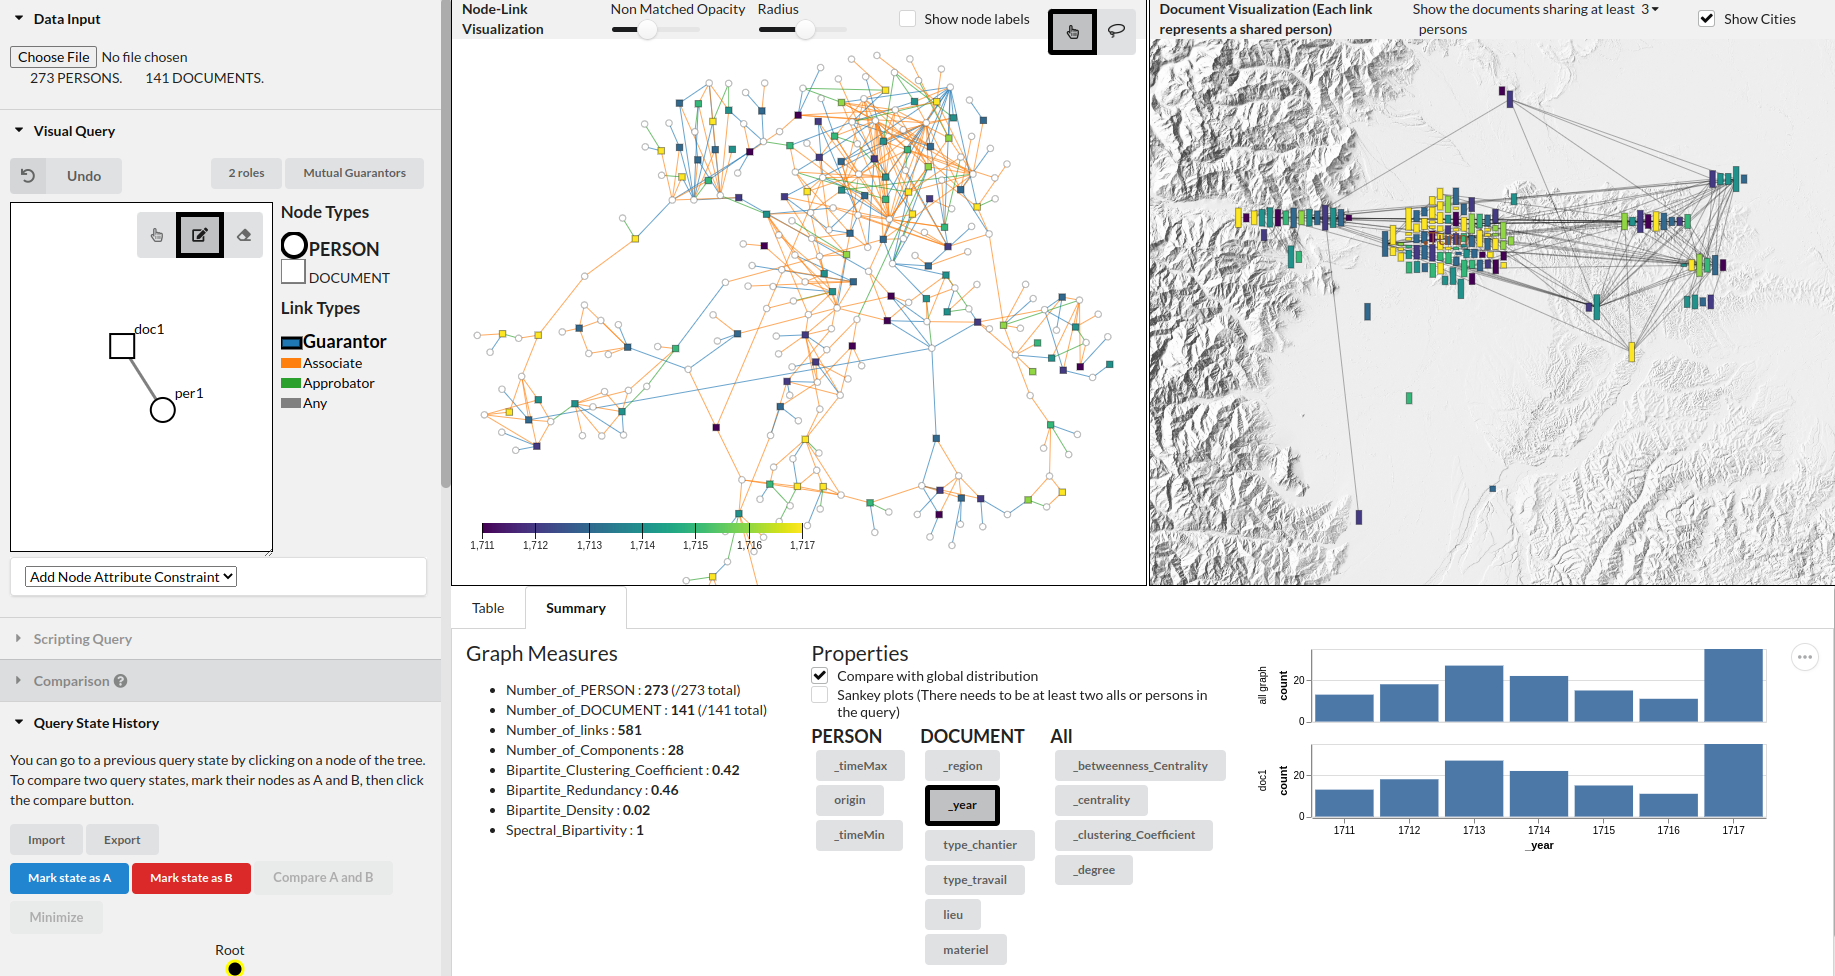
\includegraphics[trim={15.9cm 0 0 0},clip,width=\textwidth]{static/figures/ComBiNet/Piemont_timeSelected.png}
    \caption{\name interface with the dataset of collaboration \pascal. The user selected the \textit{\_year} attribute, showing the distribution of document years with a histogram (bottom right), and coloring the documents node on the bipartite view (left) and map view simultaneously (right).}\label{fig:combinet-time-selected}
\end{figure}

\subsection{Query Panel}

The query panel allows users to rapidly build queries visually, with topological and attribute constraints.
The visualization of the query is synchronized with the Cypher query sent to the database.
Modifying one representation update the other, allowing users to build a query visually and refine it in Cypher when appropriate.
Experts users who know the Cypher language can also start to construct their query textually and modify it visually later on.
In this subsection, I describe all the features and interactions allowing \name to build a query and illustrate them with questions 2 and 6 of our collaboration \pascal.
Our collaborator wants to \textit{find the persons who are mutually Guarantor to each other in separate contracts (2)} and to know \textit{how Torino and Torino's surroundings differ according to their contracts? (6)}.
\autoref{fig:visualQueriesExamples} (left) shows the final queries, but first, I explain how to create them.

\noindent\textbf{V6: Node-Link Dynamic Query}
% \todo{talk about the different links types, ego networks and paths, lasso}

The interactive node-link diagram allows the construction of a subgraph query graphically, that represents a topological constraint (T2.1).
The query subgraph is built and edited interactively.
At each modification, the visual query is converted into a Cypher query and run in the database which return the results.
All the matches are displayed in the entities tables (V3) and highlighted in the main visualizations views (V1, V2).
Three modes of interaction are available through the top-right menu: \textit{selection, addition}, and \textit{deletion}.
The \textit{selection} mode allows to drag the nodes in the panel, while the \textit{addition} and \textit{deletion} modes allow the following actions:
\begin{description}
    \item[\textbf{Node Creation:}] In \textit{addition} mode, clicking on an empty area creates a new node. The node will be of the selected type from the legend on the right (Person or Document).
    \item[\textbf{Node Deletion:}] In \textit{deletion} mode, clicking on a node deletes it and its links.
    \item[\textbf{Change Node type:}]  In \textit{selection} mode, clicking on a node opens a menu allowing to change its type.
    \item[\textbf{Link Creation:}] In \textit{addition} mode, clicking on a node and dragging the mouse to another node will connect the two with a link. Its type (color) will be the link type selected on the legend.
    \item[\textbf{Link Deletion:}] In \textit{deletion} mode, clicking on a link deletes it.
    \item[\textbf{Change link type:}] In \textit{selection} mode, clicking on a link opens a menu to change its type.
\end{description}

Users build concrete subgraphs with the same representation as in the bipartite network view: a visual query is a network template with additional attribute consraints.
Each role (link type) is rendered using a color (\autoref{fig:linkTypes} left).
Users can also create untyped links using the \textit{Any} value, which will match all the existing link types (\autoref{fig:linkTypes} left).
Created links can be matched by different selected link types, by checking several possible types for one link.
These links are represented by a dashed line with the colors of the possible types (\autoref{fig:linkTypes} middle right).
Several links with different types can also be created among two nodes to query a person with more than one role in the same event (\autoref{fig:linkTypes} right).
%All possibilities for link creation are shown in \autoref{fig:linkTypes}.
When a node or link is created in the query, it is given an identifier starting with \emph{per} for a person, \emph{doc} for a document, \emph{link} for a link, followed by a number.
These identifiers are used in the attribute constraint panels and the textual query and can be changed through their textual representations.


\begin{figure}[!ht]
    \centering
    % \begin{overpic}[width=0.6\linewidth]{static/figures/ComBiNet/OriginalPaperFigures/links/allLinks.pdf}
    % \end{overpic}
    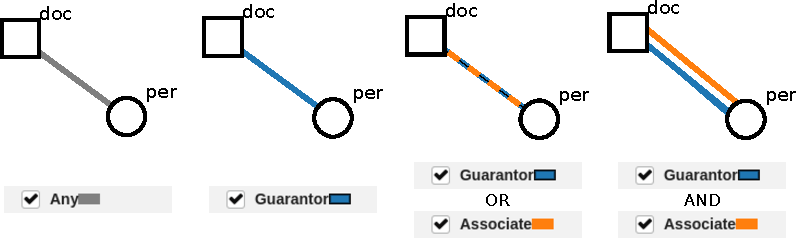
\includegraphics[width=0.9\linewidth]{static/figures/ComBiNet/OriginalPaperFigures/CGF/links.pdf}
    \caption{All link creation possibilities: Any link type (left), one selected link type, here guarantor (middle left), the union of several link types (middle right), several links with different types (right)}\label{fig:linkTypes}
\end{figure}

To find persons who are mutually guarantors in our collaboration \pascal, we first create one person and two documents using the addition mode and by clicking on the canvas.
We then link the person node to the first document with a link that is not typed (\autoref{fig:linkTypes} left), and link it to the second document with a \textit{guarantor} link (\autoref{fig:linkTypes} middle left).
We then create a second person node and link it to the two documents with opposite link types.
The resulting visual query is presented in \autoref{fig:visualQueriesExamples} (a).
To answer the question 6 (comparing Torino and Torino surroundings), we start to request all the links in the graph, no matter the type, as shown in \autoref{fig:visualQueriesExamples} (b).
The database then returns all the links in the graph with their attached nodes.
Putting attribute constraints on the location of the contracts will then let us answer the question.



\begin{figure}[!ht]
    \centering
    \begin{subfigure}[b]{0.29\linewidth}
    \centering
    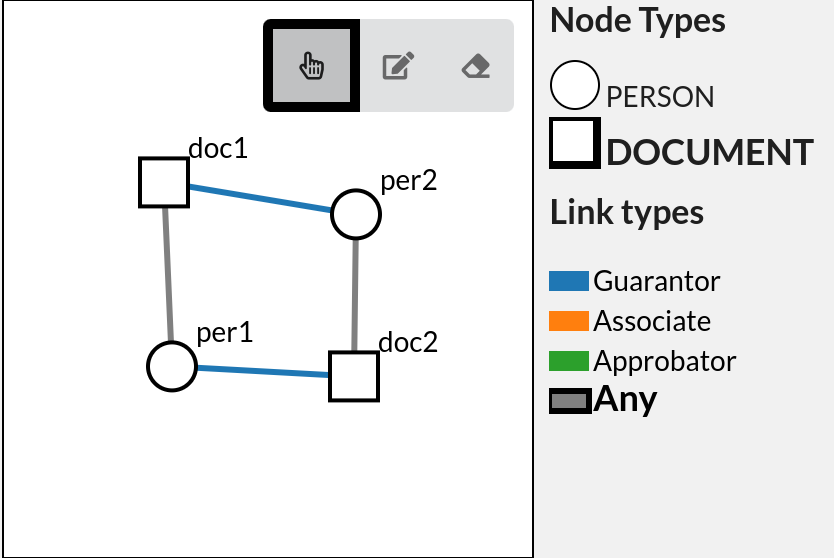
\includegraphics[width=\textwidth]{static/figures/ComBiNet/OriginalPaperFigures/CGF/MutualGuarantors.png}
    \caption{}
    \end{subfigure}
    \begin{subfigure}[b]{0.70\linewidth}
    \centering
    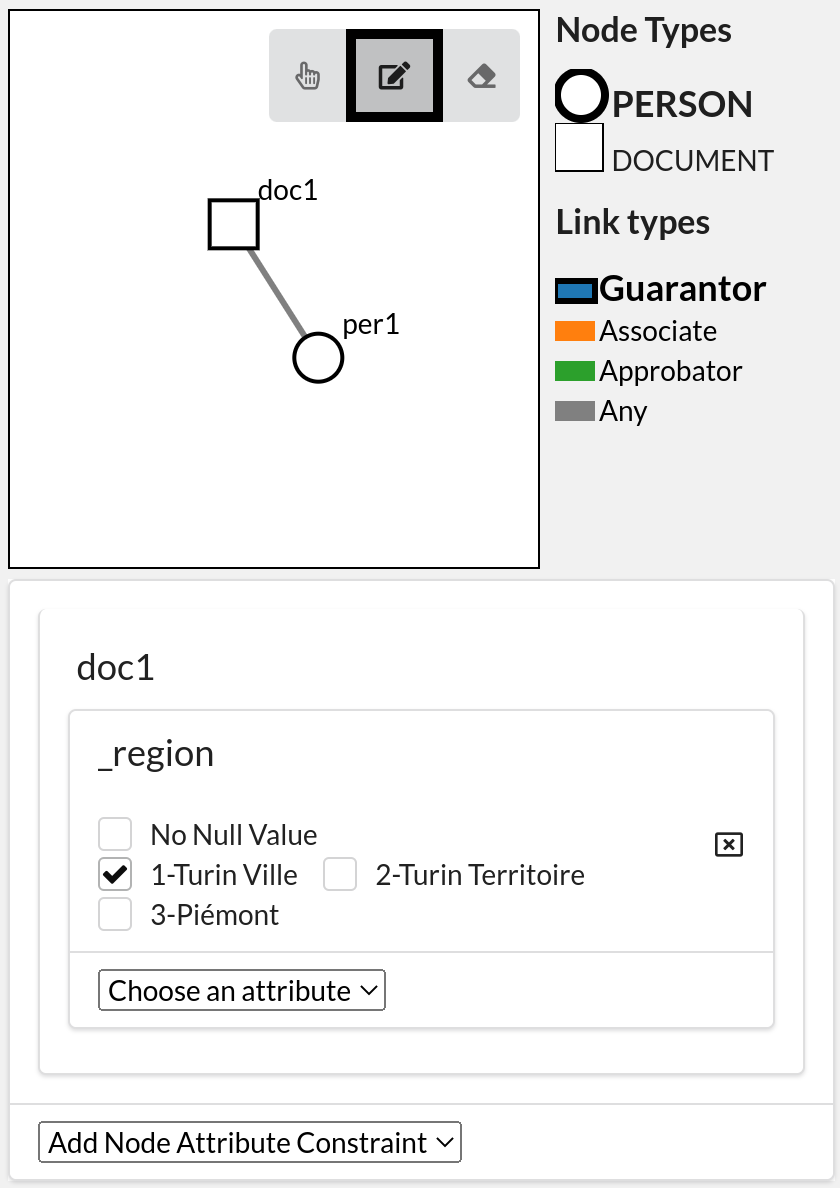
\includegraphics[width=0.46\textwidth]{static/figures/ComBiNet/OriginalPaperFigures/CGF/Turin.png}
    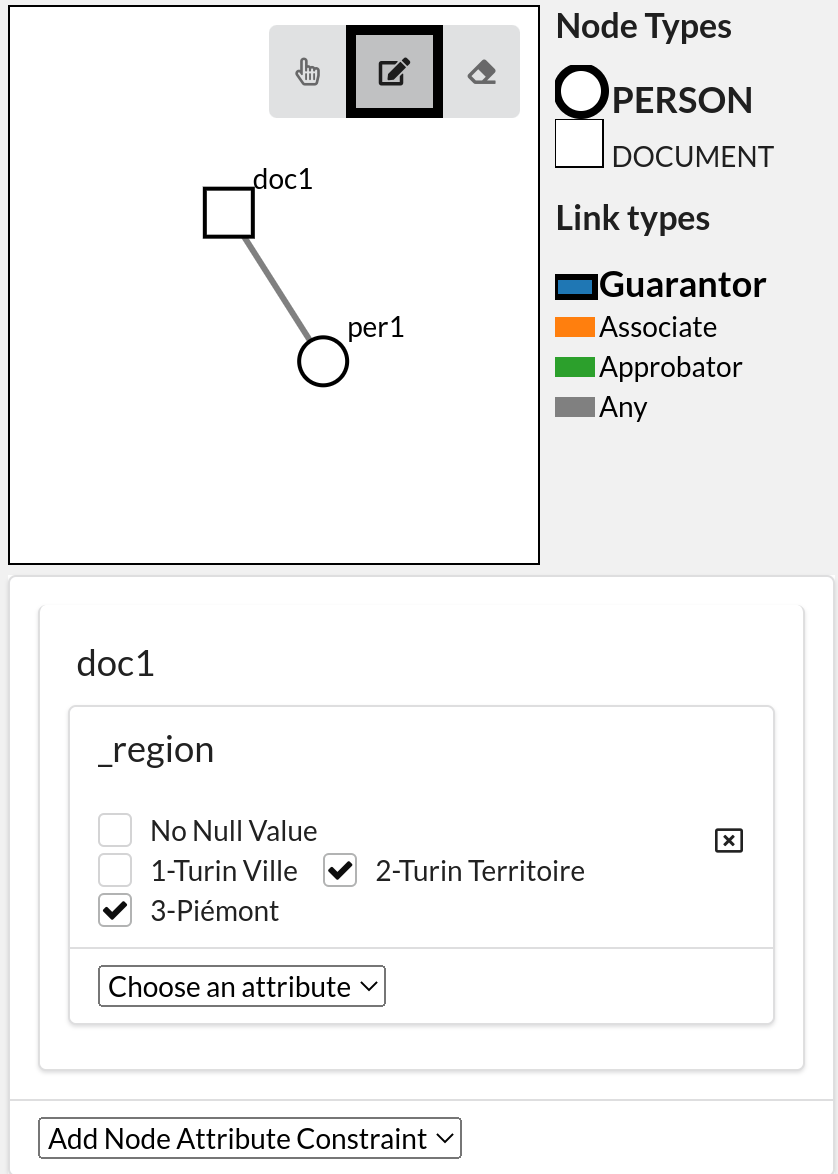
\includegraphics[width=0.46\textwidth]{static/figures/ComBiNet/OriginalPaperFigures/CGF/TurinoSuburbs.png}
    \caption{}
    \end{subfigure}

    \caption{Visual queries created to answer questions 2 and 6 of our collaboration \pascal. (a) The visual query retrieves individuals who are mutually guarantor to each other in separate construction contracts.
        (b) The two visual queries retrieve the documents---along with the signatories---of Torino (\textit{Turin} in french) (left) and of Torino surroundings (\textit{Turin Territoire} and \textit{Piemont}) (right)}\label{fig:visualQueriesExamples}
\end{figure}


%\iffalse
%\begin{figure}
%    \centering
%
%    \begin{overpic}[trim=60 60 60 60, width=0.2\linewidth]{static/figures/ComBiNet/OriginalPaperFigures/NL01}
%    \put(55, 12) {\circled{1}}
%    \end{overpic}
%    \begin{overpic}[trim=60 60 60 60, width=0.2\linewidth]{static/figures/ComBiNet/OriginalPaperFigures/NL02}
%    \put(55, 12) {\circled{2}}
%    \end{overpic}
%    \begin{overpic}[trim=60 60 60 60, width=0.2\linewidth]{static/figures/ComBiNet/OriginalPaperFigures/NL03}
%    \put(55, 12) {\circled{3}}
%    \end{overpic}
%    \begin{overpic}[trim=60 60 60 60, width=0.2\linewidth]{static/figures/ComBiNet/OriginalPaperFigures/NL04}
%    \put(55, 12) {\circled{4}}
%    \end{overpic}
%
%    \caption{Steps to create a new node and link in the node-link diagram. 1: Initial query of one document. 2: Creation of one person node by click. 3: Creation of one Approbator (marked A, green link) link by click and drag. 4: The link between the document and the person has been created after mouse release.}\label{fig:NodeLinkCreation}
%\end{figure}
%\fi



\noindent\textbf{V7: Attribute Constraint Widgets}\label{sec:attributes}
Users can also add attribute constraints (T2.2) on the created nodes with the help of interactive widgets.
An input button is created for each node and link identifier from the node-link query panel.
It allows to create a dynamic query widget for any of its attributes.
% When selected, it initialize a constraint visualized by a widget users can interactively modify.  The possible choices of attributes depend on the node type (person or document).
The widget design vary according to the three possible attribute types: numeric, categorical, and nominal, as in the original dynamic queries formalization by Shneiderman~\cite{DynamicQueries}:
\begin{enumerate}
    \item \textbf{Numeric constraints} are modeled as range sliders, allowing the selection of lower and upper bounds to the filter.
    \item \textbf{Categorical constraints} are modeled as a set of checkboxes. Each possible value has a corresponding checkbox.
    \item \textbf{Nominal constraints} are modeled as text input, where the user can write any desired value. All the possible values are shown at the same time and filtered as the user writes.
\end{enumerate}

For the categorical and nominal widgets, selecting several values corresponds to the union of the filters.
The three widget types are shown in \autoref{fig:combinet-widgets}.

\begin{figure}[!ht]
    \centering
%    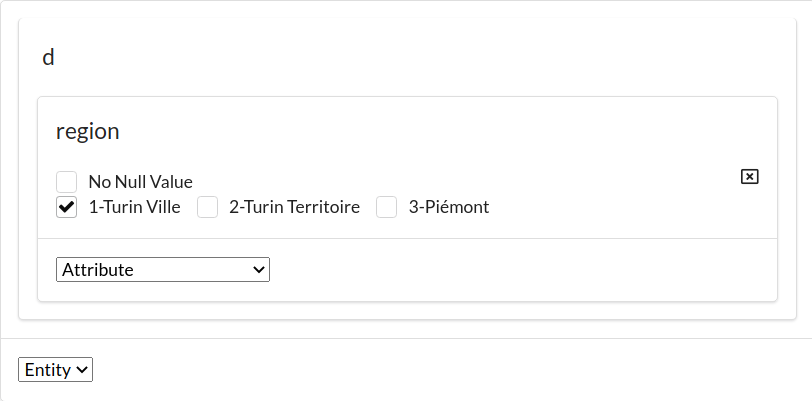
\includegraphics[trim=30 145 300 110,clip,width=0.8\linewidth]{static/figures/ComBiNet/OriginalPaperFigures/constraintRegion.png}%
    % 
\includegraphics[width=0.8\linewidth]{static/figures/ComBiNet/OriginalPaperFigures/categoricalWidget}
    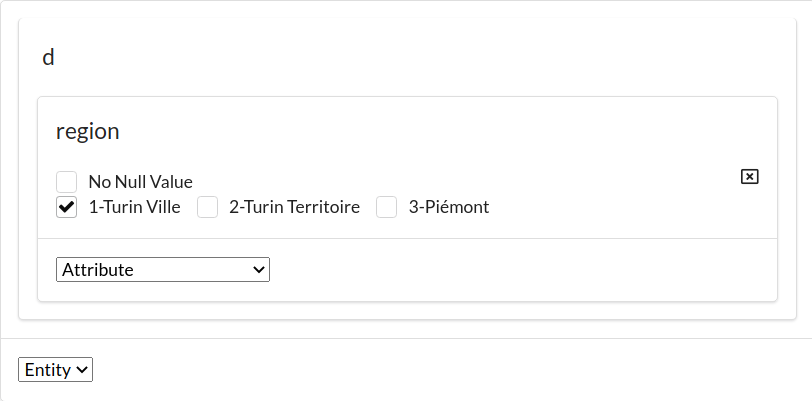
\includegraphics[width=0.7\linewidth]{static/figures/ComBiNet/OriginalPaperFigures/constraintRegion.png}\\
    
\includegraphics[width=0.6\linewidth]{static/figures/ComBiNet/OriginalPaperFigures/nominalWidget}\\
    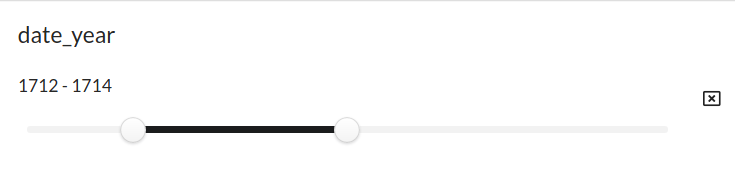
\includegraphics[width=0.6\linewidth]{static/figures/ComBiNet/OriginalPaperFigures/numericWidget}

    \caption{Widget designs for the different attribute types: checkboxes for categorical attributes (top), text input for nominal attributes (middle), and a double slider for numerical attributes (bottom). The categorical attribute example shows the  inputs letting users create new constraints for other attributes and other nodes.}\label{fig:combinet-widgets}
\end{figure}
%\fi

To answer our collaborator's second question (\textit{how do Torino and Torino's surroundings differ according to their contracts?}), we first filter the documents which are located in Torino (\textit{Turin}).
For this, we select the whole dataset by linking a person and document node with an untyped link.
Then, we select the id \textit{doc1} of the document of our visual node-link query, and the \textit{region} attribute.
It initializes a categorical widget including all the values found in the dataset for this attribute with associated checkboxes.
We check the region of interest ``\textit{1-Turin Ville}'' to select all the documents from this region.
 The first widget of \autoref{fig:combinet-widgets} illustrates the created constraint.
To select the documents of Torino's surroundings, we can simply uncheck the ``\textit{1-Turin Ville}'' value for the \textit{region} attribute and check the two other values ``\textit{2-Turin Territoire}'' and ``\textit{3-Piemont}'' which are areas corresponding to the surroundings of Torino.
Both queries are represented in \autoref{fig:visualQueriesExamples} (b).


\noindent\textbf{V8: Cypher Editor}
Users can build or modify a query using the Cypher query language, with the Cypher text editor.
This allows users to start creating a query visually and refining it by text for complex constraints which can not be represented by a visual form easily.
The parts of the Cypher query which are not visually expressible appear in Cypher widgets next to the other widgets.
The editor supports autocompletion to e.g., help to discover and spell the attribute names.
The visual and textual representations are synchronized, meaning that modifying one update the other and return the results in the visualizations, tables, and attribute distributions.


\noindent\textbf{Query Results}
Each modification of the query, whether from the node-link dynamic query, the widgets, or the Cypher text box, update the two visualization panels (V1, V2), the entities tables (V3), the network measures view (V5), and the attribute plots (V6).
The nodes and links that do not match (are not retrieved by the query) are grayed out in V1 and V2 and are removed from the persons and documents tables (V3).
A third table shows every occurrence found of the created pattern that we call the occurrence table.
The occurrence table for question 1 of collaboration \pascal is shown in \autoref{fig:combinet-example-results} (a).
It tells us that the occurrence has been found 72 times, meaning that the pattern exists 36 times in the network by taking into account the symmetry of the subgraph query.
Users can switch between the three tables in the table view using the tabs.
The network measures are computed on the new subgraph formed by the union of all patterns found and updated on the network measures view (V5).
\autoref{fig:combinet-example-results} (b) (left) shows to the user the different graph measures of the subgraph induced by the patterns found.
Since some measures can be long to compute, the values are computed iteratively in the backend and shown progressively~\cite{feketeProgressiveDataAnalysis2019} to avoid blocking the interface.
The distribution plots in the attributes view (V6) are updated, showing the values of the entities of the latest constructed query, next to the global distributions.
%By selecting the \textit{origin} attribute as seen in \autoref{fig:combinet-example-results} (b) (right)

% Each modification of the query, whether from the node-link dynamic query, the widgets, or the Cypher text boxes, update the two visualization panels. The nodes and links that do not match (are not retrieved by the query) are grayed out. It allows to rapidly visualize the subset of entities resulting from the applied query while maintaining the context.
% The results are shown in detail in the results section panel, constituted of the results tables and summary tabs, both shown in \autoref{fig:ResultsSection}. The table shows each occurrence of the query pattern found in the graph, with details on demands. Clicking on a row shows every attribute of the matched entities. Users can select a set of rows to highlight and visualize the occurrences directly in the two graph views.

% The summary tab presents graph measures computed from the subgraph resulting from the union of all occurrences of the queried pattern, such as the number of persons, documents, bipartite density, and the bipartite clustering coefficient. For the specified query, 42 documents are localized in Torino, 99 persons are mentioned in these contracts 153 times (given by the number of links).

\begin{figure}[!ht]
    \centering
    \begin{subfigure}[b]{\linewidth}
        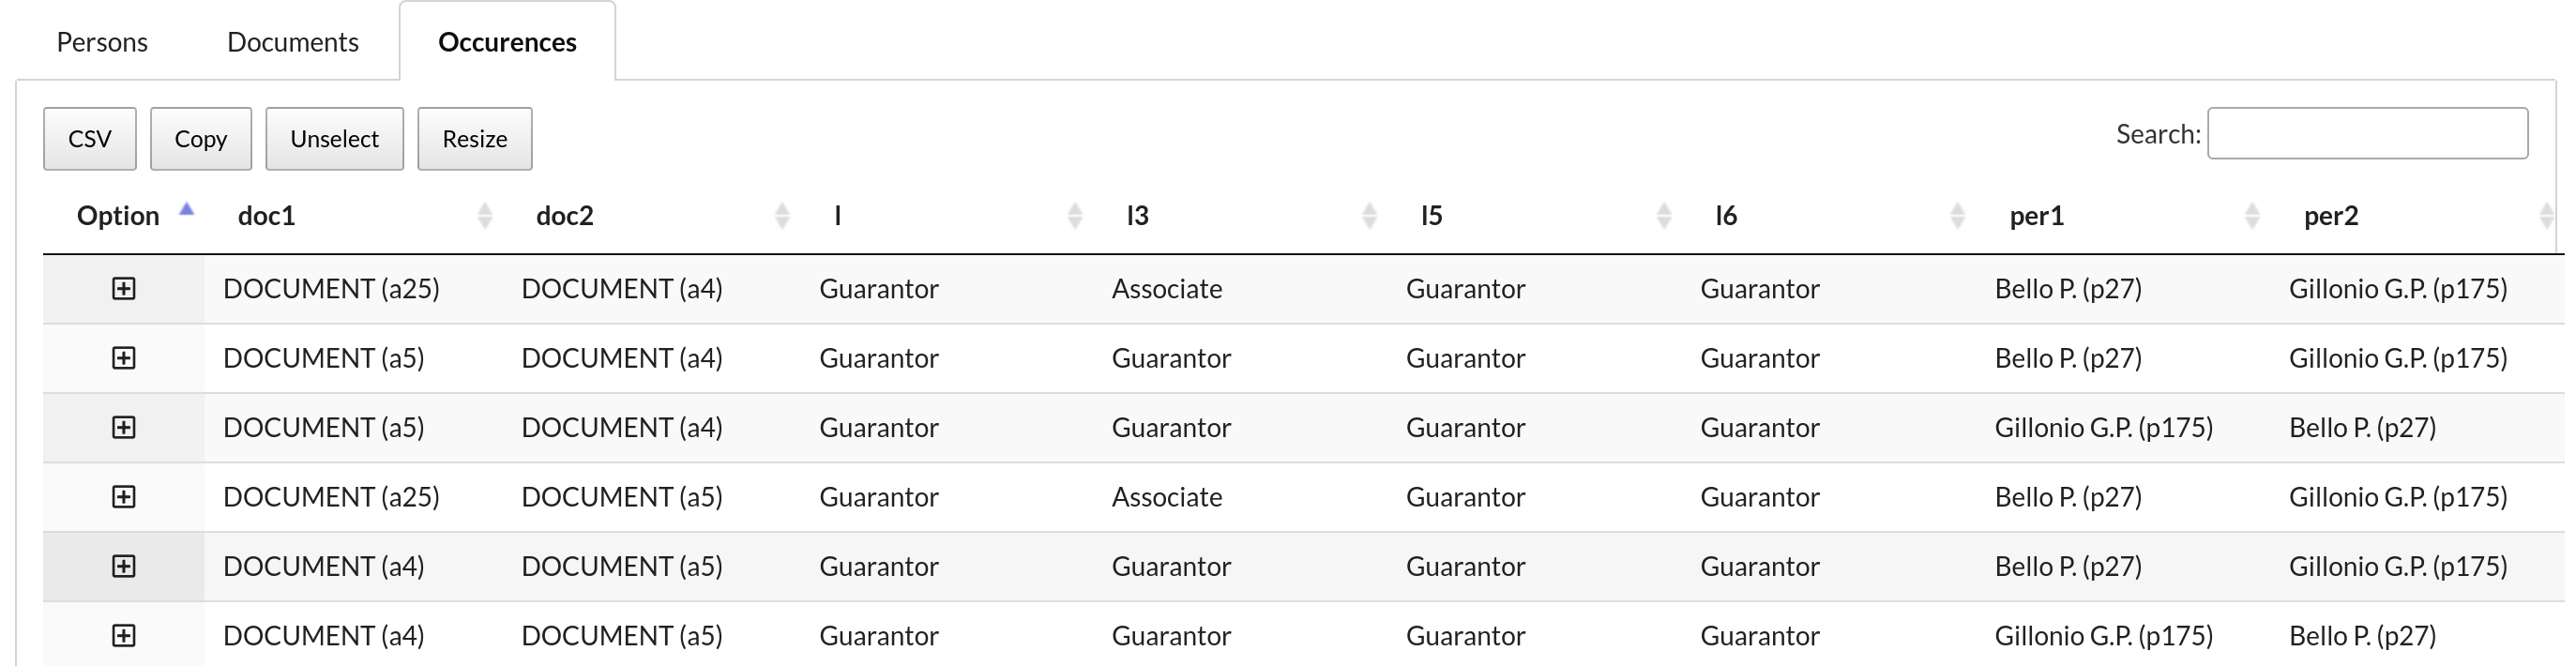
\includegraphics[width=\textwidth]{static/figures/ComBiNet/Piemont-mutual-guarantor-table}
        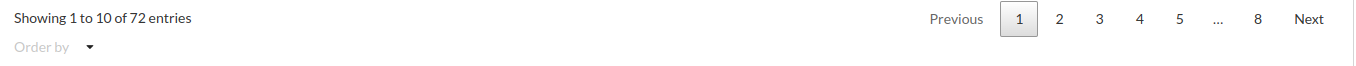
\includegraphics[width=\textwidth]{static/figures/ComBiNet/mutualGuarantor-table-bottom}
    \caption{}
    \end{subfigure}

    \begin{subfigure}[b]{\linewidth}
            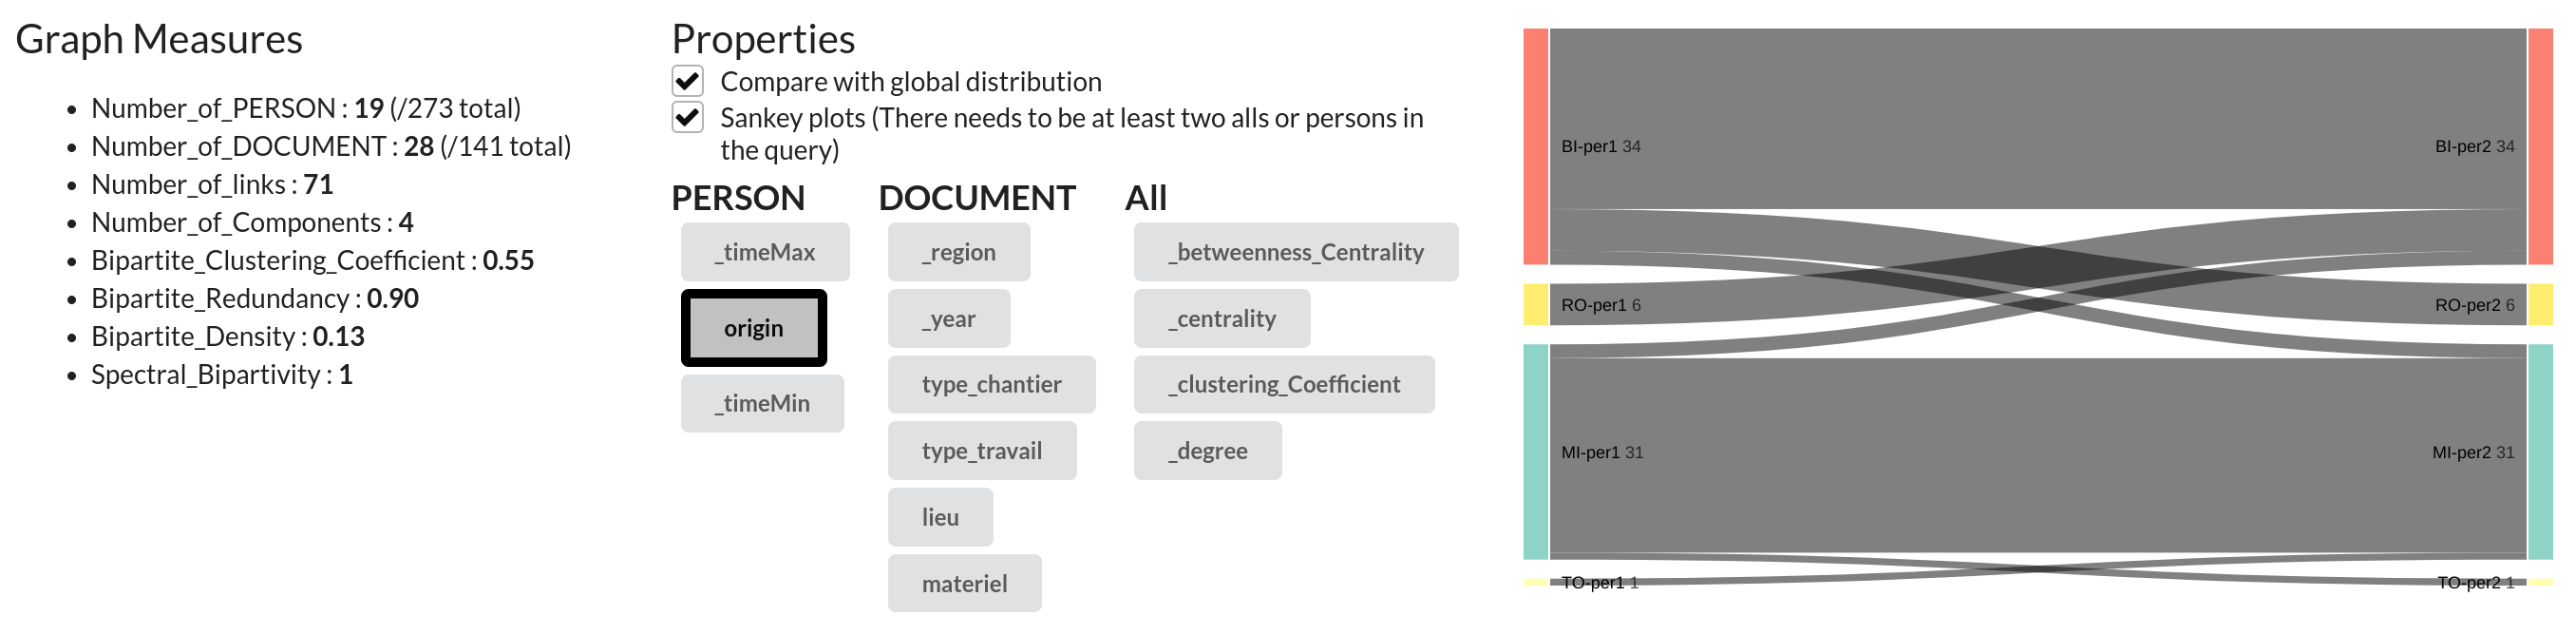
\includegraphics[width=\textwidth]{static/figures/ComBiNet/piemont-mutual-guarantors-results}
    \caption{}
    \end{subfigure}

    \caption{Results of question 2 of collaboration \pascal: (a) shows a subset of the table view with every occurrence of the pattern found. (b) shows the summary panel, with the graph measures and the attributes view with the \textit{origin} attribute selected and the Sankey option checked. It allows us to see the attribute distribution of the persons included in the pattern and see if there is a relationship between persons who are mutually guarantors and their origin.
%    bioglio BI
%    Comune di Ro
%    MI Milano
    }\label{fig:combinet-example-results}
\end{figure}


\noindent\textbf{Attributes Visualization} When users select an attribute in the attributes view (V5), its distribution is visualized for the queried entities and the whole network with an histogram.
However, these plots show the aggregated values and we lose the potential value transitions between the query nodes.
For example, \autoref{fig:sankeys} shows a query to list the persons with the role of ``approbator'' (green) in a contract after being a ``guarantor'' (blue) in another contract (using a time constraint).
We may want to see if the locations or types of the two contracts are the same or if they change, case by case.
Unfortunately, we lose this information with the aggregated plots.
By checking the ``Sankey'' option on top of the distribution visualization, the plots are transformed into Sankey diagrams, giving information on how the attribute values relate between the nodes (person or event) of the same query.
% The given query example along the distribution of the \textit{type chantier} in both a stacked bar chart and Sankey diagram is shown in .
A Sankey diagram showing the attribute distributions is particularly useful for queries where nodes have a relationship in regard to time, such as birth certificates, marriage, or death certificates where we know the order in which these events occurred.
It is also useful for queries with user-defined time order constraints as in \autoref{fig:sankeys}.


\begin{figure}[!ht]
    \centering

    \begin{subfigure}[b]{0.24\linewidth}
    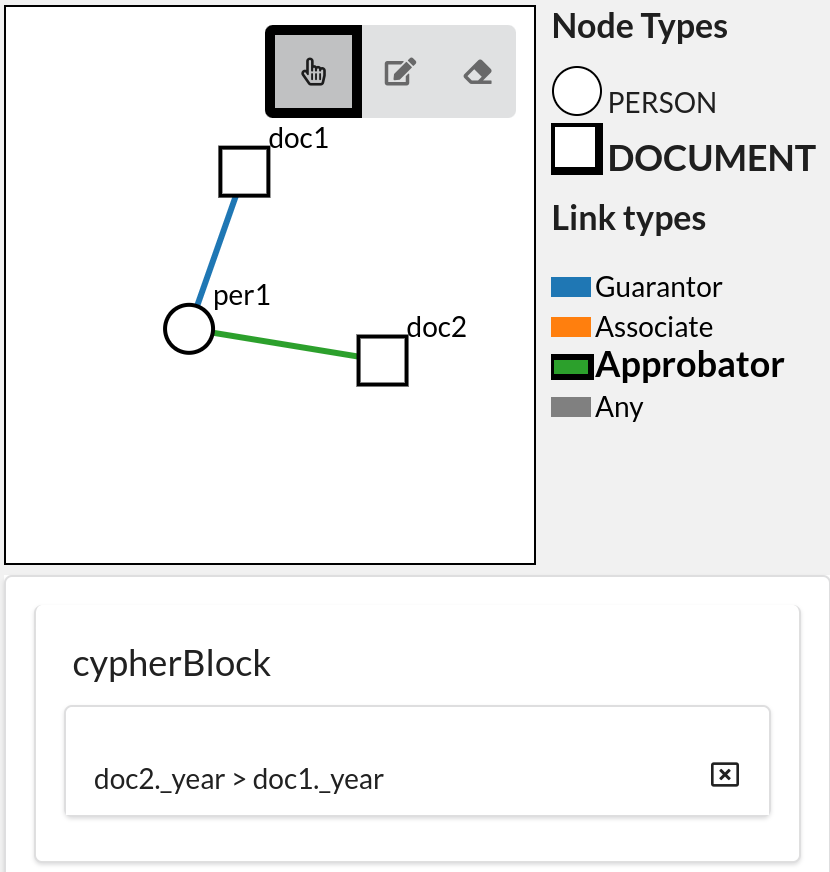
\includegraphics[width=\textwidth]{static/figures/ComBiNet/OriginalPaperFigures/CGF/sankeyPLot/apprGuar.png}
    \caption{}
    \end{subfigure}
    \begin{subfigure}[b]{0.3\linewidth}
    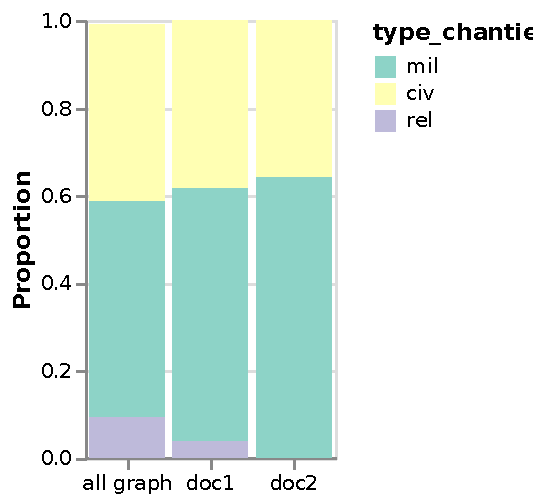
\includegraphics[width=\textwidth]{static/figures/ComBiNet/OriginalPaperFigures/CGF/sankeyPLot/barchart.pdf}
    \caption{}
    \end{subfigure}
    \begin{subfigure}[b]{0.44\linewidth}
    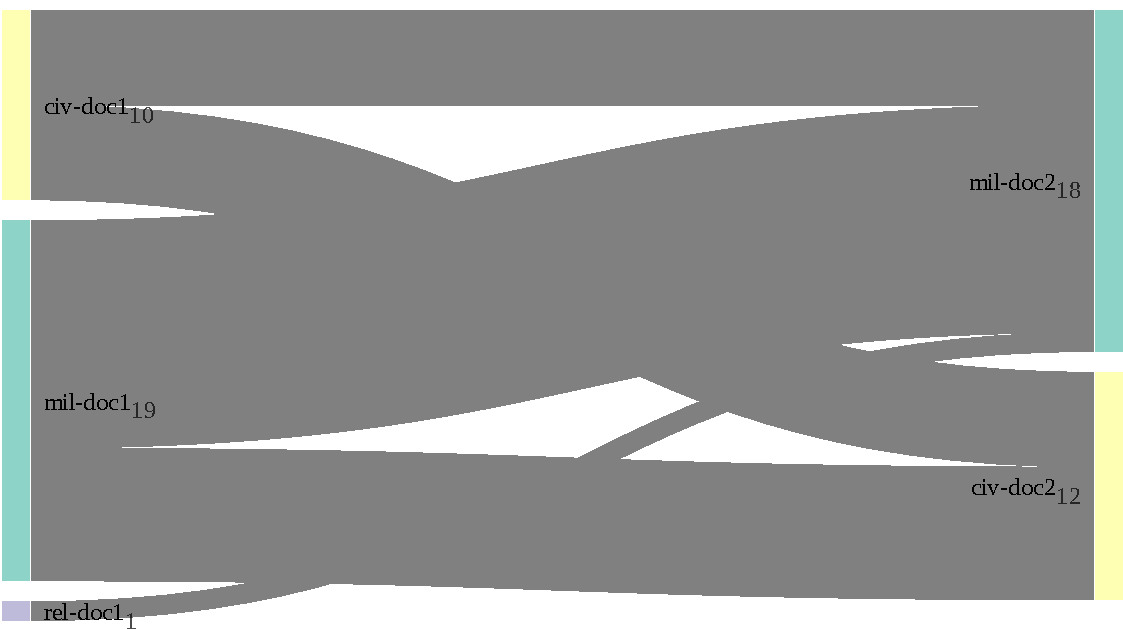
\includegraphics[width=\textwidth]{static/figures/ComBiNet/OriginalPaperFigures/CGF/sankeyPLot/sankey_bigger.pdf}
    \caption{}
    \end{subfigure}
    \caption{Two ways of showing the distribution of ``type chantier'' (type of works), a categorical attribute with three possible values ``\textsl{rel}igious'', ``\textsl{mil}itary'', and ``\textsl{civ}ilian''.
    (a) A query matching the contracts made by the same person (\textit{per1}) as an ``approbator'' (green link to \textit{doc2}) after being a ``guarantor'' (blue link to \textit{doc1}) using the constraint (\texttt{doc2.\_year > doc1.\_year}). (b) Stacked bar chart for the matches, the earlier contract (\textit{doc1}), the older contract (\textit{doc2}), and (c) Sankey diagram with the early values on the left and the last on the right.
    The Sankey diagram reveals the value changes between the two documents: the guarantor who worked initially on religious work switched to military work.} \label{fig:sankeys}
\end{figure}

The graph measures and attribute views for the results of question 2 of collaboration \pascal are shown in \autoref{fig:combinet-example-results}.
The Sankey view of the \textit{origin} attribute shows that mutual guarantors come from 4 regions only and that usually, people have mutual guarantor relationships only with persons of the same origin.
This is especially true for persons from \textit{Milano}, and with some reciprocal links between persons from \textit{Bioglio} and the \textit{Comune di Ro}.

% \begin{figure}
%     \centering
%     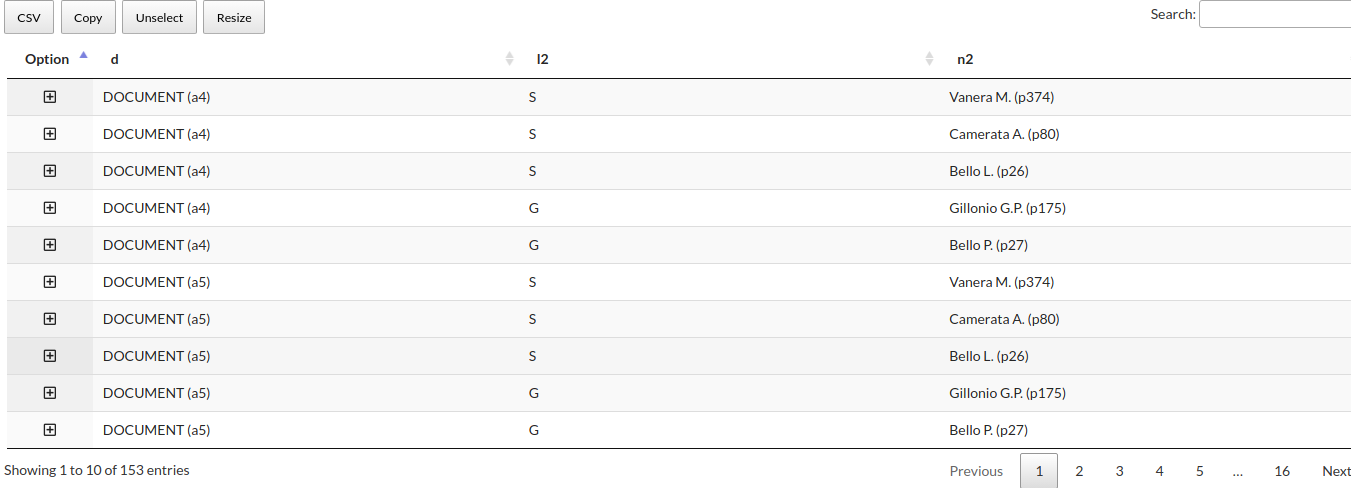
\includegraphics[width=0.99\linewidth]{static/figures/ComBiNet/OriginalPaperFigures/TableExample}
%     \caption{The table tab of the result panel shows every pattern which matched with the constructed query. Clicking on the plus button shows details on the matched nodes, and users can select specific occurrences to highlight them in the graph view and center the view around them.}\label{fig:ResultsSection}
% \end{figure}

% \begin{figure}[b]
%     \centering
%     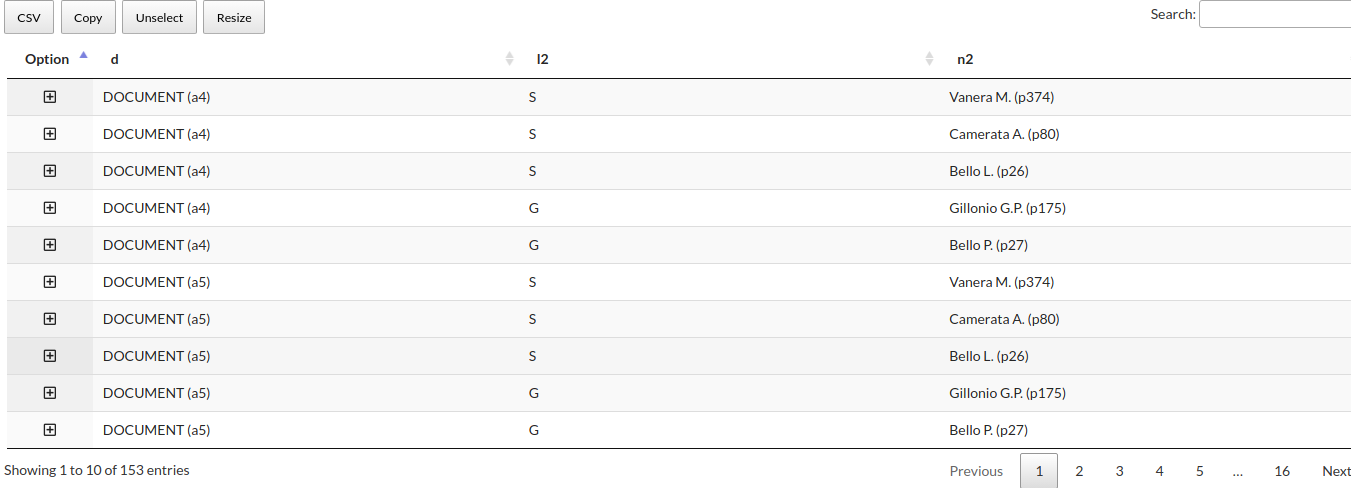
\includegraphics[width=0.99\linewidth]{static/figures/ComBiNet/OriginalPaperFigures/TableExample}
%     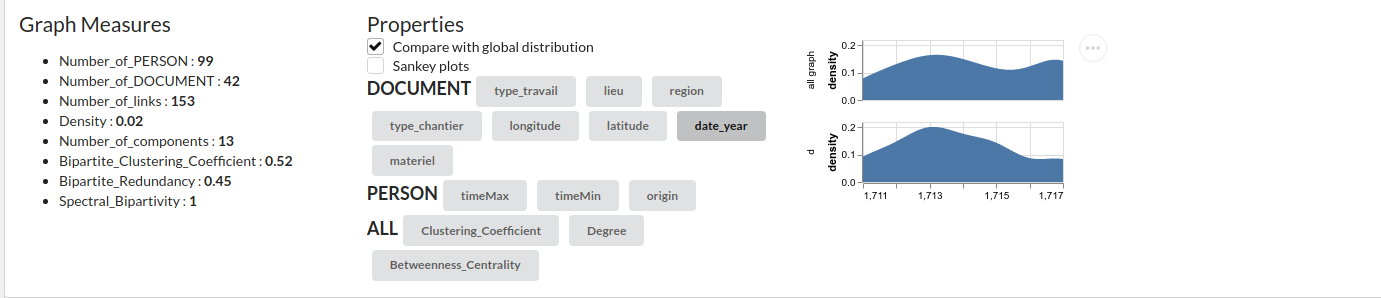
\includegraphics[width=0.99\linewidth]{static/figures/ComBiNet/OriginalPaperFigures/SummaryExample}
%     \caption{The detailed results panel shows a table (top) and summary tab (bottom) of the request specified in the query panel. The table shows each match of the query, while the summary presents graph measures for the graph elements matching the query, along with the distributions of the attributes. Here, the user selected the \textit{date\_year} attribute; the distributions show that the distribution of the selection is similar to the distribution of the whole graph.}\label{fig:ResultsSection}
% \end{figure}


\noindent\textbf{V9: Provenance Tree}
Each change in the query panel is saved with the computed results so that the history of the query construction can be shown in the form of a provenance tree (T2.4), managed with the Trrack library~\cite{cutlerTrrackLibraryProvenanceTracking2020}.
Each node of the tree represents a query change, with a description label such as ``New Link''.
It allows to rapidly visualize the succession of filters applied with their refinements.
At any moment, users can rename a tree node or click on it to go back to the previous state; allowing them to explore different query possibilities easily and iteratively.
Hovering over a node shows a tooltip with the query panel associated with the selected query state.
It let users rapidly see what query is associated with each node of the tree
If a new change is made on the query from a previous state, a new branch is created on the tree, allowing to revisit and refine explorations.  \autoref{fig:combinet-trees} shows the provenance tree made to answer question 2, split into 2 branches, with the tooltip showing one of the node query state.

\begin{figure}[!ht]
     \centering
%     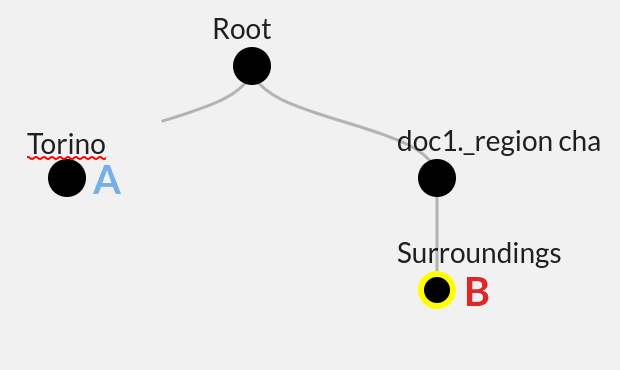
\includegraphics[width=0.3\linewidth]{static/figures/ComBiNet/torino_tree}
     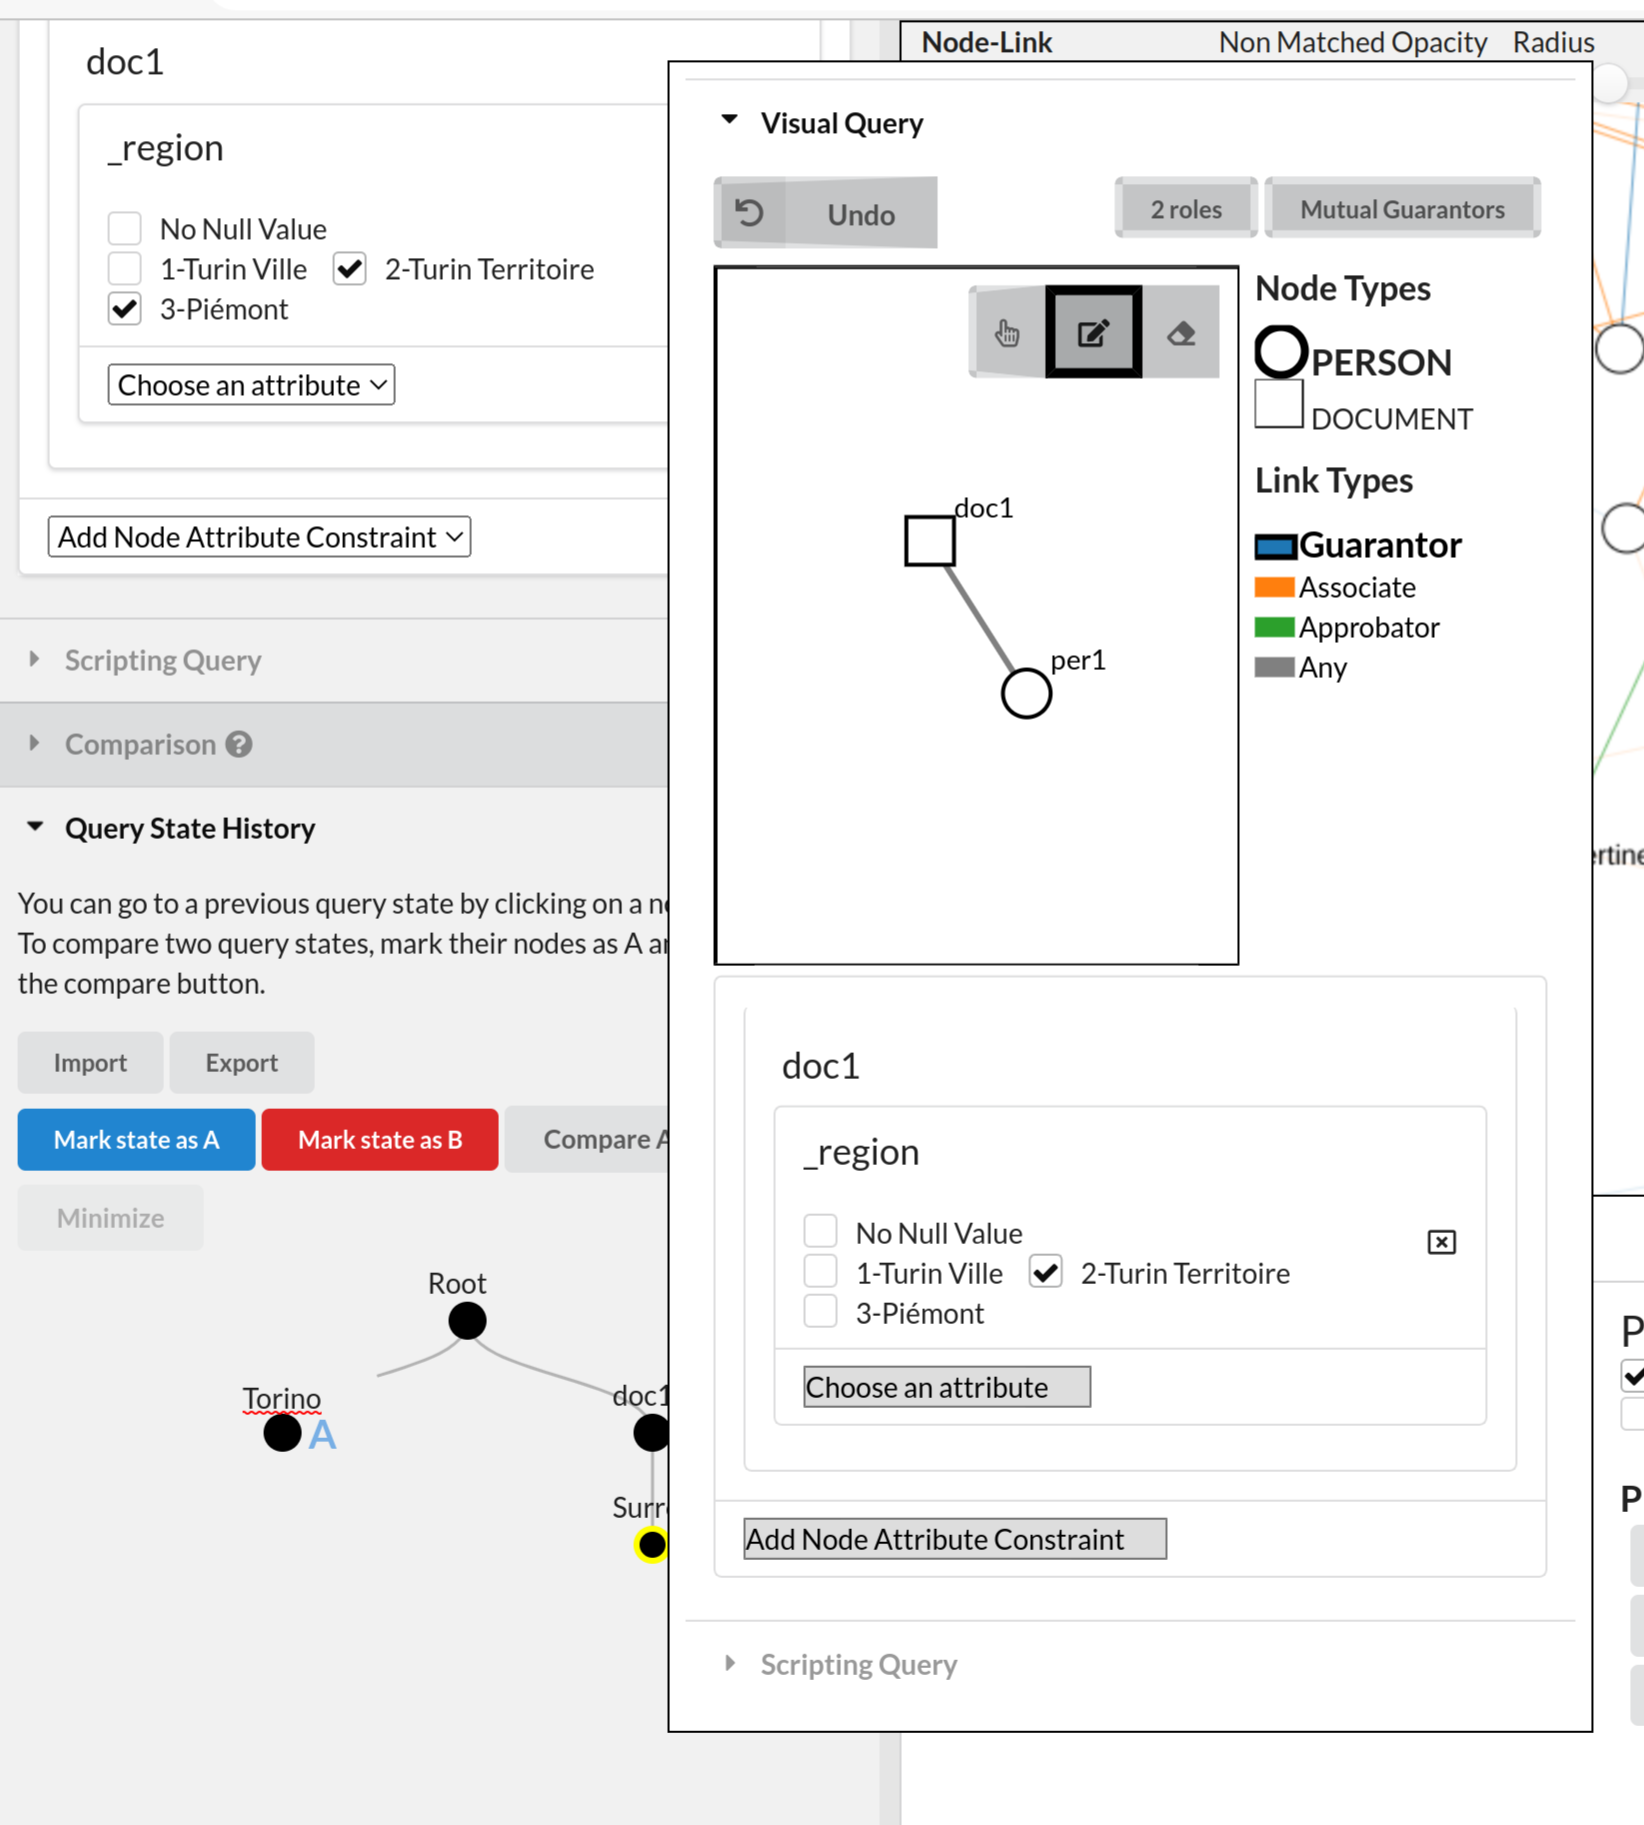
\includegraphics[width=0.5\linewidth]{static/figures/ComBiNet/tree_tooltip_torinoquery_crop}
%     \caption{(a) Provenance tree to answer question 2 of collaboration \pascal: left branch lead to Torino documents (the node is labeled as A) while right branch lead to surrounding documents (the node is labeled as B). }\label{fig:combinet-trees}
     \caption{Provenance tree to answer question 2 of collaboration \pascal: left branch leads to Torino documents (the node is labeled as A) while right branch leads to surrounding documents (the node is labeled as B). The user hovers over one node, revealing a tooltip that shows the visualization of the node's query..}\label{fig:combinet-trees}
 \end{figure}


\subsection{Comparison}

In addition to comparing the results of a query to the whole graph, \name allows comparing the results of two queries.
Users can select two query states in the provenance tree and mark them either as ``A'' or ``B''.
Clicking on the button ``Compare State A and B'' compares them.
The interface changes to \emph{comparison mode}.
Several buttons appear on top of the provenance tree: $A$, $B$, $A-B$, $B-A$, $A \cap B$, and $A \cup B$ for exploring the combinations of the two results of A and B in the two visualizations panels.

To answer several of the questions raised by our collaborators, we need to compare two subsets of the network.

In the question 6 of collaboration \pascal, we want to compare the constructions in Torino with the ones in Torino surrounding.
Since we previously constructed the query returning all the contracts from Toriono (\textit{Turin}) with the mentioned people, we can
return to this point in the provenance tree, and change the constraint of the \textit{region} attribute from \textit{Turin} to \textit{Turin Territoire} and \textit{Piemont} using the checkboxes to get the documents of Torino surroundings in a second query.
Both queries are shown in \autoref{fig:visualQueriesExamples} (b).
The user can then rename the provenance tree nodes with explicit names such as ``Torino'' and ``Surroundings'', and mark them as A and B using the appropriate buttons.
Clicking on the ``Compare State A and B'' will make the interface compare the two query results.


% \begin{figure}
%     \centering
%     % \includegraphics[width=0.2\linewidth]{static/figures/ComBiNet/OriginalPaperFigures/query01.png}
%     % \includegraphics[width=0.2\linewidth]{static/figures/ComBiNet/OriginalPaperFigures/query02.png}
%     % \includegraphics[width=0.2\linewidth]{static/figures/ComBiNet/OriginalPaperFigures/query03.png}
%     % \includegraphics[width=0.2\linewidth]{static/figures/ComBiNet/OriginalPaperFigures/query04.png}
%     \includegraphics[scale=0.1]{static/figures/ComBiNet/OriginalPaperFigures/CGF/MutualGuarantors.png}
%     \includegraphics[scale=0.1]{static/figures/ComBiNet/OriginalPaperFigures/CGF/Turin.png}
%     \hspace{-8pt}
%     \includegraphics[scale=0.1]{static/figures/ComBiNet/OriginalPaperFigures/CGF/TurinoSuburbs.png}
%     \caption{Queries to answer our collaborator's four questions.
%     % Visual queries made to find back the four patterns our collaborator is interested in.
%     }\label{fig:queries}
%     \vspace{-8pt}
% \end{figure}

\noindent\textbf{Topological Comparison}
In comparison mode,
% the two graph visualization panels do not change but
users can rapidly switch between the visual filters of (A) and (B) by hovering over their respective buttons on the comparison menu and thus compare the structure of the two resulting subgraphs (T3.1).
Similarly, different boolean comparison operations are available by hovering their respective buttons (\autoref{fig:combinet-overall}-C), such as the intersection, union, and differences between the two filters. % It allows to rapidly change filters to find interesting persons or group of persons in a exploratory process.
Moreover, the summary tab allows comparing the different graph measures of the two subgraphs by showing them side by side (T3.3).
\autoref{fig:combinet-comparisonTable} shows the comparison table for the queries returning the subgraph of Torino (A) and Torino surroundings (B).
% as shown in \autoref{fig:comparisonTable}.
Comparing these measures, such as the number of matched documents or the densities, is crucial for \sna.
For example, the table indicates that the density is two times higher for Torino, suggesting that less persons paticipate in the same construction compared to Torino surroundings.

\begin{figure}[!ht]
    \centering
%    \includegraphics[width=0.8\linewidth]{static/figures/ComBiNet/OriginalPaperFigures/comparisonPlots/graphMeasuresComparison.png}
    \includegraphics[width=0.8\linewidth]{static/figures/ComBiNet/graph_measures_Torino_territoireandpiemont}
  \caption{Comparison table of the networks measures for Torino subgraph (A) and Torino surroundings subgraph (B).}\label{fig:combinet-comparisonTable}
\end{figure}

%\todo{comparaison de torino et territoire sur le graphe} ?

\noindent\textbf{Attribute-Based Comparison}
The comparison of one or several attribute distributions between (A) and (B) is also useful for answering the historical questions of our users.
In the attribute view (V5) of the results panel, hovering or clicking on an attribute name will show the distribution of this attribute in four contexts: the nodes of the whole graph, the queries (A), (B), and the currently selected Boolean operator (e.g., intersection or union) if one is selected.
This allows users to compare attribute distributions between several subsets of interest (T3.2).
For example, we can compare the attributes between the contracts of Torino and the ones of its surroundings.
We can also compare the persons who worked in Torino, in Torino's close territory, and in both areas, by selecting the intersection operator.
% or the persons who collaborated in those regions, if we select the intersection operator.
\autoref{fig:attributeComparison} illustrates the comparison plots for different attributes.
The first plot indicates that the types of construction sites differ between the two regions: the city of Torino clearly has a lot of military sites compared to the surroundings of Torino, which has almost none.
This is the opposite for the number of religious sites, which are almost all localized in the surroundings of Torino.
If we now look at the year distribution of the contracts, we can see a difference in the distributions.
The years of Torinos's construction contracts were steady between 1711 and 1717 with a little spike in 1713, while the constructions were more scarce in the surroundings before 1716.
We can see a big spike in construction in 1717.
This is interesting to our users, as it shows the dynamic of the construction in the area: the center of the city started to be constructed before other constructions arose in the surroundings.
%The majority of Torino's contracts occurred around 1713 and around 1717 for Torino's surroundings.

We can also compare the profiles of persons who collaborated at Torino and Torino surroundings by selecting the intersection of those two queries.
One of the questions the historian had (question 2 of \autoref{tab:tasks}) was to know if those persons were a group with specific attributes and characteristics, or were inseparable from other persons working in the two areas.
If we look at the betweenness centrality, on average, the values are higher for this group of people, meaning that the persons who work on the construction site at Torino and Torino's territory are clearly two distinct groups, and the persons collaborating in the two areas act as bridges between these groups.
This visual demonstration was convincing and revealing for our users.

\begin{figure}[!ht]
    \centering

    % \includegraphics[width=0.2\linewidth]{static/figures/ComBiNet/OriginalPaperFigures/comparisonPlots/type_chantier}
    % % \includegraphics[width=0.2\linewidth]{static/figures/ComBiNet/OriginalPaperFigures/comparisonPlots/type_travail}
    % \includegraphics[width=0.2\linewidth]{static/figures/ComBiNet/OriginalPaperFigures/comparisonPlots/date_year}
    % \includegraphics[width=0.2\linewidth]{static/figures/ComBiNet/OriginalPaperFigures/comparisonPlots/Betweeness_Centrality}

    % \includegraphics[height=90px]{static/figures/ComBiNet/OriginalPaperFigures/comparisonPlots/type_chantier}
    % % \includegraphics[width=0.2\linewidth]{static/figures/ComBiNet/OriginalPaperFigures/comparisonPlots/type_travail}
    % \includegraphics[height=90px]{static/figures/ComBiNet/OriginalPaperFigures/comparisonPlots/date_year}
    % \includegraphics[height=90px]{static/figures/ComBiNet/OriginalPaperFigures/comparisonPlots/Betweeness_Centrality}

    \includegraphics[height=90px]{static/figures/ComBiNet/OriginalPaperFigures/CGF/TurinPlots/type+chantier.pdf}
    \includegraphics[height=90px]{static/figures/ComBiNet/OriginalPaperFigures/CGF/TurinPlots/time.pdf}
%    \includegraphics[height=90px]{static/figures/ComBiNet/OriginalPaperFigures/CGF/TurinPlots/centrality.pdf}
    \includegraphics[height=90px]{static/figures/ComBiNet/TorinoCompBC.pdf}

    \caption{Distribution of the type of constructions, the years, and the betweenness centrality for the documents and signatories of Torino (A), Torino surroundings (B), and the whole graph (top).}\label{fig:attributeComparison}
%    \caption{Distribution of two document attributes and one global attribute for the documents and signatories of Torino (A), Torino surroundings (B), and the whole graph. (top).}\label{fig:attributeComparison}
\end{figure}


\subsection{Implementation}

\name is made of three components: a web visual interface, a python server, and a Neo4j\cite{neo4j} graph database instance.
The client interface is written in JavaScript using D3~\cite{d3}, Vega~\cite{satyanarayan2016vega}, and the Trrack library~\cite{cutlerTrrackLibraryProvenanceTracking2020}.
The python server is written in Flask and interacts with the Neo4j instance for query processing before sending the results to the frontend.
We implemented the Cypher parser with the ANTLR parser generator~\cite{parr1995antlr}.
The abstract syntax tree of the Cypher query is used as a representation of the query.
Modifying the query visually update the tree, which is translated into Cypher in the textual query panel.
Similarly, a manual change in the Cypher query update the abstract syntax tree which is translated into a visual query.

%\todo{Talk about AST and implementaion}


\section{Use Cases}\label{sec:combinet-usecases}

In this section, we describe  how our system has been able to specifically answer questions from two of our collaborations.
the tool was mostly operated by the developers working side by side with the collaborators to test the expressiveness of the queries and the value of the results visualizations.
The tool was refined as needed along the way.

% Since usability issues have not been resolved yet, the tool was mostly operated by the developers working side by side with the collaborators to test the expressiveness of the queries and the value of the results visualizations. The tool was refined as needed along the way.

\subsection{Construction sites in Piedmont (\#1)}

One of the main questions of our collaborator was to compare two families which he knew played a big role in the structure of the network: the \textit{Menafoglio} and \textit{Zo} families (question 4 in \autoref{tab:tasks}).
Specifically, he was interested in knowing if there were differences in specialization in type of contracts and area of work for the core members of these families, and to what extent the two families were collaborating.
Moreover, he was very interested in characterizing the group of people collaborating with both families.

To answer those questions, we first selected the core members of the \textit{Menafoglio family}, by checking the people known by the historian, and their close neighbors.
Looking at the bipartite view (see Figure 1 of the supplementary material), we can see that the group is pretty dense with people collaborating a lot between them.
Looking at the map, we can clearly see that the family has been mostly active in Piedmont outside of Torino and Torino's close territory.
We also have a first view of the attribute distribution of the persons in the group and their contracts.

We then do the same query for the Zo family. We keep the same topological filter and replace the name filters with the core members of the Zo family known by the historian. We see on the graph view (Figure 2 of the supplementary material) that the group is smaller and is in a different area in the graph. The map enriched with a selection of the \textit{region} attribute shows that, contrary to the Menafoglio, the Zo family has been more active in Turin and around.

The two groups can be compared using the \textit{comparison mode} by selecting the two queries in the provenance tree. This opens the comparison menu to quickly navigate between the visual selection of (A), (B), and the set $A \cap B$ that interests our collaborator. The table showing the graph measures of the two subsets confirms what is shown visually: the Menafoglio group is more populated but less dense than the Zo family.

Our user is then interested in comparing the distribution of several attributes between the two groups. We can clearly see in \autoref{fig:useCasePascal} (middle) that the Menafoglio family is more specialized in military sites, while the Zo family is doing more civil construction. This is confirmed by the ``material'' distribution that shows that the contracts of the Menafoglio are often using stones, whereas it is never the case for Zo contracts. Finally, the persons collaborating in the two groups have a betweenness centrality higher on average. This makes sense as they act as bridges linking the two families.
% Moreover, we can see in detail the difference in the region of contracts of the two families.


\begin{figure}[!ht]
    \centering

    % \includegraphics[height=70px]{static/figures/ComBiNet/OriginalPaperFigures/CGF/MenaZoPlots/materiel.pdf}
    %  \includegraphics[height=70px]{static/figures/ComBiNet/OriginalPaperFigures/CGF/MenaZoPlots/type_chantier.pdf}
    %  \includegraphics[height=70px]{static/figures/ComBiNet/OriginalPaperFigures/CGF/MenaZoPlots/type_travail.pdf}
    %   \includegraphics[height=80px]{static/figures/ComBiNet/OriginalPaperFigures/CGF/MenaZoPlots/BC_crop.pdf}

    \includegraphics[width=0.3\linewidth]{static/figures/ComBiNet/OriginalPaperFigures/CGF/MenaZoPlots/v2/region.pdf}
     \includegraphics[width=0.3\linewidth]{static/figures/ComBiNet/OriginalPaperFigures/CGF/MenaZoPlots/v2/type-chantier.pdf}
     \includegraphics[width=0.3\linewidth]{static/figures/ComBiNet/OriginalPaperFigures/CGF/MenaZoPlots/v2/materiel.pdf}
     %\includegraphics[width=0.35\linewidth]{static/figures/ComBiNet/OriginalPaperFigures/CGF/MenaZoPlots/v2/BC_crop.pdf}

    \caption{Attributes distributions plots between the whole graph, the \textit{Menafoglio} family (A), the \textit{Zo} family (B), and $A\cap B$, for the \textit{region,type\_chantier,  material type.}
    % , and \textit{betweeness centrality}.}
    \label{fig:useCasePascal}}
\end{figure}

% \begin{figure*}
%     \centering

%     \begin{overpic}[width=0.15\linewidth]{static/figures/ComBiNet/OriginalPaperFigures/useCase01/queryMena.png}\end{overpic}
%     \begin{overpic}[width=0.15\linewidth]{static/figures/ComBiNet/OriginalPaperFigures/useCase01/queryZo.png}
%     \end{overpic}
%     \begin{overpic}[width=0.6\linewidth]{static/figures/ComBiNet/OriginalPaperFigures/useCase01/comparisonRegionNoZoom.png}
%     \end{overpic}

%     \caption{}\label{fig:useCasePascal}
% \end{figure*}


% \begin{figure*}
%     \centering

%     \begin{overpic}[width=\linewidth]{static/figures/ComBiNet/OriginalPaperFigures/useCase01/queryAndComparePascal}

%      \put(30,14){\small Comparison}
%     %  \put(25, 22){\circled{\large A}}
%     \put(25, 4){\circled{\large I}}
%      \put(40, 4){\circled{\large II}}
%     \end{overpic}

%     \includegraphics[height=120px]{static/figures/ComBiNet/OriginalPaperFigures/useCase01/attributes/materiel.pdf}
%     %  \includegraphics[width=0.2\linewidth]{static/figures/ComBiNet/OriginalPaperFigures/useCase01/attributes/region.pdf}
%      \includegraphics[height=120px]{static/figures/ComBiNet/OriginalPaperFigures/useCase01/attributes/type_chantier.pdf}
%      \includegraphics[height=120px]{static/figures/ComBiNet/OriginalPaperFigures/useCase01/attributes/type_travail.pdf}
%      \includegraphics[height=120px]{static/figures/ComBiNet/OriginalPaperFigures/useCase01/attributes/betweenness.pdf}

%     \caption{Comparison of the two group of interests for use case \pascal. (I) shows the two queries the user created to select the two groups of interest. (II) presents \name in comparison mode, with the intersection of (A) and (B) selected. The table shows the structural difference of the two groups, while the two graph views highlight the persons who collaborated between the two groups, who are of interest for our collaborator. The user selected the \textit{region} attribute, creating a plot showing that the Menafoglio and Zo families are working respectfully more in Piemont and Torino, while their collaboration has no strong associated region.}  \label{fig:useCasePascal}
% \end{figure*}

%\vspace{-1mm}
\subsection{French Genealogy (\#2)}

We describe how \name allowed us to answer an important question of the use case \nicole: to detect the largest migrations across several generations, in which areas, and at what time they occurred (question 7 in \autoref{tab:tasks}).
The map view shows at a glance (Figure 3 in the supplementary material) that the majority of events have taken place in three specific regions west, mid-north, and mid-south.

To find patterns of migrations within families, we first make a query representing a simple family by linking a person node to a birth event, connected to the parents using a link of \textit{father} or \textit{mother} type. We repeat the process to the new parent node to add another generation. Finally, we connect the latest generation child with a death event, to have another date and location to compare to (see \autoref{fig:UseCaseNicoleQ}). This query returns every person with their parents and grandparents, along with their respective birth and death data for the latest person. We also create a constraint on the \textit{department} attribute on the documents to only retrieve the events that have a non-null associated location. This request returns a subgraph of 64 persons and 88 documents. The user can now select the \textit{department} attribute to create a Sankey diagram that shows the change of departments across the different generations of the families. \autoref{fig:UseCaseNicoleS} shows that the majority of families are from \textit{Haute-Vienne} (which can easily be confirmed by checking the map), and do not move much across generations. Our collaborator however detected interesting patterns of people moving from the department \textit{Creuse} to \textit{Haute-Vienne} across two generations. She refined the query by adding an attribute filter on this specific department using a widget. The table view then showed her who these migrants were and when it occurred. The bipartite visualization panel allowed exploring more in-depth this specific group of people. %, with their close neighbors.


% We now can use the Sankey visualization of the \textit{department} attribute to see if there is interesting patterns of migration.
\begin{figure}[!ht]
    \centering
    % \begin{subfigure}{0.49\linewidth}
    % \includegraphics[width=\textwidth]{static/figures/ComBiNet/OriginalPaperFigures/useCase02/queryParents3gen.png}
    % \caption{Visual query to find all 3-generation families (documents without department have been filtered out)}
    % \label{fig:UseCaseNicoleQ}
    % \end{subfigure}
    % % \includegraphics[width=0.4\linewidth]{static/figures/ComBiNet/OriginalPaperFigures/useCase02/armorConstraint.png}
    % \begin{subfigure}{0.49\linewidth}
    % \includegraphics[width=\textwidth]{static/figures/ComBiNet/OriginalPaperFigures/useCase02/sankey3genDep.pdf}
    % \caption{Sankey diagram showing the birthplace of people across generations and the death place}
    % \label{fig:UseCaseNicoleS}
    % \end{subfigure}

    \begin{subfigure}[b]{0.4\linewidth}
    \includegraphics[width=\textwidth]{static/figures/ComBiNet/OriginalPaperFigures/CGF/frenchGenealogy/migrationQuery.png}
    \caption{Visual query to find all 3-generation families %(only documents mentioning a department are shown)
    }
    \label{fig:UseCaseNicoleQ}
    \end{subfigure}
    % \includegraphics[width=0.4\linewidth]{static/figures/ComBiNet/OriginalPaperFigures/useCase02/armorConstraint.png}
    \begin{subfigure}[b]{0.59\linewidth}
    \includegraphics[width=\textwidth]{static/figures/ComBiNet/OriginalPaperFigures/CGF/frenchGenealogy/migration3.pdf}
    \caption{Sankey diagram showing the birth and death places of people across generations}
    \label{fig:UseCaseNicoleS}
    \end{subfigure}

    \caption{Migrations across departments over three generations}  \label{fig:useCaseNicole}
\end{figure}

Afterward, we answered question 8 (\autoref{tab:tasks}),
% of our user closely related to the first one.
to compare the migrations between the 18th and 19th centuries. She thought people started moving in the 19th century and wanted to confirm it. To answer this, we first created a query to retrieve the people with birth and death certificates from a specified department. We then applied a time filter on the death certificate node, first for the 18th century and then the 19th century, compared the two query results using the comparison mode, and looked side by side the Sankey graphs related to \textit{departments} (\autoref{fig:useCaseNicole2}). We can clearly see that people do not move at all in the 18th century, while in the 19th century even if the majority of people stay in the same place from their birth to their death, more than half moved.%  It thus confirms the hypothesis of our collaborator.

\begin{figure}[!ht]
    \centering
    % \begin{subfigure}{0.49\linewidth}
    % \includegraphics[width=\textwidth]{static/figures/ComBiNet/OriginalPaperFigures/useCase02/sankeyDep18c.pdf}
    % \caption{18th century}
    % \end{subfigure}
    % \begin{subfigure}{0.49\linewidth}
    % \includegraphics[width=\textwidth]{static/figures/ComBiNet/OriginalPaperFigures/useCase02/sankeyDep19c.pdf}
    % \caption{19th century}
    % \end{subfigure}

    \begin{subfigure}{0.49\linewidth}
    \includegraphics[width=\textwidth]{static/figures/ComBiNet/OriginalPaperFigures/CGF/frenchGenealogy/migration_18.pdf}
    %\caption{18th century}
    \end{subfigure}
    \begin{subfigure}{0.49\linewidth}
    \includegraphics[width=\textwidth]{static/figures/ComBiNet/OriginalPaperFigures/CGF/frenchGenealogy/migration_19.pdf}
    %\caption{19th century}
    \end{subfigure}

    \caption{Sankey diagrams showing the migration of people in the 18th and 19th centuries, extracted from their birth and death places.}\label{fig:useCaseNicole2}
\end{figure}

\subsection{Marriage acts in Buenos Aires (\#3)}

I present in this subsection how \combinet has been used to detect erroneous encoding during the annotation process of the marriage acts.
The documents mention 6659 individuals, whom can have the same name, especially between fathers and sons in this period and region as specified by our collaborator.
During the annotation process, the historian and his collaborators gave identifiers to the persons mentioned in the documents---which is the common annotation procedure.
However, for this case of homonyms, it can be hard to know if some mentions between different documents refer to the same or different persons.
Historians cross the information contained in the different documents to disambiguate the persons\cite{winchesterLinkageHistoricalRecords1970}, but errors can easily be made, \ie giving the same identifier to different persons or giving different identifiers to the same person.
I used \combinet in collaboration with researchers of this project to detect erroneous patterns and help them refine their encoded data.
%For this, we created a query to detect persons mentioned in two acts either as \textit{husband}, \textit{wife}, or \textit{witness} with a time difference of 70 years or more.
For this, we can find the persons mentioned in two acts either as \textit{husband}, \textit{wife}, or \textit{witness} with a time difference of 70 years or more.
Such person nodes in the network are with almost full certainty representing two different persons who lived in different generations.
We constructed a request to find this pattern with the visual query view and added the time constraint between the two marriage acts with the Cypher textual input.
%returning this pattern visually and added the time constraint between the two marriage acts with the Cypher view.
\autoref{fig:combinet-BuenosAires-correction} shows the visual query constructed (left), the bipartite view with the persons and documents matching the query highlighted (middle), and the table listing all the documents having mentions of people with erroneous identifiers (bottom right).
%The query returned 29 persons found in this pattern.
The table permit to browse through all persons nodes (29 have been found) who correspond in fact to more than one person and to the documents which contain the wrongly given identifiers.
Using the exporting capabilities, our collaborator have exported the occurrence table indicating him with their identifiers the pairs of documents mentioning two different persons who have been given the same identifier.
Using this table, he has been able to rapidly correct those errors in his annotation framework.

\begin{figure}[!ht]
    \centering
    \includegraphics[width=\linewidth]{static/figures/ComBiNet/BuenosAires_correction}
    \caption{\name used to request persons appearing as husband, wife, or witness in two marriages which occurred at 70 years apart or more.}\label{fig:combinet-BuenosAires-correction}
\end{figure}


% 54 occurence, 71 documents, 29 persons
%MATCH (mar2:MARRIAGE_ACT)-[l3:HUSBAND|WIFE|WITNESS]-(per1:PERSON)-[l:WIFE|HUSBAND|WITNESS]-(mar1:MARRIAGE_ACT) where mar1._year - mar2._year > 70 RETURN *
%6659 PERSONS. 1381 MARRIAGE_ACTS




\subsection{Sociology thesis in France}

I describe in this third use case how \name can be used to answer questions about thesis in France between 2016 and 2022.
Indeed, some sociological datasets made of documents can also be well modeled as \modelplural like for example thesis dissertations: a thesis is a document with specific attributes such as the subject, the doctoral school, the domain, the university, and the date of defense, and mention several peoples who are socially connected through the thesis defense with different roles: author (\textit{auteur} in french), director(s) (\textit{directeur}), referees (\textit{rapporteur}), and jury president (\textit{président de jury}).
%We discussed with sociologists who were interested in this type of data for explorations purposes.
We present here an exploration of the data by ourselves using \name.
A first look at the graph measures tells us that 896 theses have been defended in sociology in France between 2016 and 2021 in France, with 2453 persons included in the defenses (see \autoref{fig:combinet-thesis-exploration} bottom).
The bipartite node-link view shows us an overview of the network but is hard to parse due to the network's size.
Zoom actions though allow centering the view for specific parts of the network.
The map view allows us to see that theses has been defended all around France, even though the majority are defended in Paris.
This is confirmed by a look at the distribution of the cities (\autoref{fig:combinet-thesis-exploration} bottom right): around half of the defenses are in Paris, compared to the rest of the country which is more or less homogeneous.
By setting the threshold to link creation to one (meaning that a link is created between two documents if they mention at least one common person), a lot of links are created as seen in \autoref{fig:combinet-thesis-exploration} (right).
It means that a lot of thesis defenses include referees and juries from different cities.


\begin{figure}[!ht]
    \centering
    \includegraphics[width=0.8\textwidth]{static/figures/ComBiNet/Thesis-first-exploration}
    \caption{\name used for exploring theses of sociology defended in France between 2016 and 2021. The bipartite and map views show an overview of two visions of the network. The user selects the \textit{region} attribute, showing the geographical distribution of the defended thesis.}\label{fig:combinet-thesis-exploration}
\end{figure}

Let's now try to answer an interesting question: ``Do referees and jury presidents often ask thesis directors to be referees and jury presidents in their turn of another thesis where they are directors ?''.
For this, we can construct a visual query representing this pattern by creating two person nodes and two document nodes, and by connecting them with two president links and two referee or jury director links in a symmetrical way, as shown in \autoref{fig:combinet-thesis-query} (right).
The occurrence table tells us that this pattern has been found 76 times in the network, meaning that this is a recurrent behavior.
We are now interested in characterizing the thesis occurring in this pattern, by their regions.
We can look at the \textit{city} attribute distribution for this thesis by selecting it in the attribute view as shown in \autoref{fig:combinet-thesis-query} (bottom right).
We can first see on the map that this pattern occurs mainly in the biggest cities of the country.
By selecting the Sankey view option, we can investigate if this pattern occurs between thesis defended in different regions or if it occurs mainly in the same ones.
We learn that it depends mainly on the regions: in Bourgogne-Fanche-Comté 26 out of 29 theses are connected with the thesis of another region.
On contrary, in \textit{Occitanie} it is the case for only 4 out of 17.
On average, we can see that this pattern occurs a lot for theses of the same region.
In Ile-de-France, it is the case for around half of the thesis (28/50).
This exploratory analysis shows that \name can be used to explore and gain insight into such datasets.



\begin{figure}[!ht]
    \centering
    \includegraphics[width=0.8\textwidth]{static/figures/ComBiNet/Thesis-query01-and-results}
    \caption{Sociology thesis dataset explored with \name. The user constructed a visual query to see if there are symmetrical relationships between thesis directors and referees (or jury directors). The \textit{region} attribute is selected with the Sankey option, letting the user see if there are correlations between the regions of the thesis found in this pattern.  }\label{fig:combinet-thesis-query}
\end{figure}



% \subsection{Feedback}

% After a few iterations, we showed the final system to two of our collaborators during
% a three hours session. We answered their questions step by step while describing the process and the interface.
% They also took part in the analysis by asking new questions on their data, leading to new explorations and discussions.

% Both of them liked the Sankey view of the attributes, allowing them to see the evolution of distributions and answering several of their questions. Our collaborator of the use case \nicole\ was making sense of it by linking the migration patterns she was seeing in the Sankey view with specific persons of the dataset she knew in depth. She was also curious about other migration patterns she was not aware of, and wanted to know who these persons were, the system allowing her to select them and follow a deeper exploration.

% Both liked the export capabilities of the system to collect results in CSV or JSON format, as well as the charts in SVG, for inclusion in their publications or for processing with other tools.


\section{Formative Usability Study}\label{sec:combinet-usability}

%\subsection{Procedure}

% After showing our tool can be used to answer socio-historical questions,
We performed a formative usability study with two historians and one expert in visualization. We had 3 meetings with each and gave them control of the tool to see if they could use it to explore their data and perform queries and comparisons. At each meeting, we asked them to speak aloud, commenting on their aims and actions. At the end of each session, we asked them their general feedback and what other features they would like to have. We improved the system and made the changes asked by the users before setting up new appointments. This usability study led to the redesign of some core features, like the activation of the comparison mode which is now started by first marking the state nodes in the provenance tree. It also led to the implementation of new features, such as the person and document tables (which are updated after each query), the persistent selection of nodes across the two views and the tables, and the undo feature for visual queries.
% The list of all feedback and modifications are shown in the supplementary material.
At the final meetings, the three users were able to perform exploration, queries, and comparisons to answer socio-historical questions by themselves.


%\vspace{-1mm}
\subsection{Feedback}

All three users liked the table views and were exploiting them to study in depth who were the person and documents found in their specific queries.
Both historians liked the Sankey diagram of the attributes, allowing them to see the evolution of distributions and answering several of their questions. Our collaborator of the use case \nicole was making sense of it by linking the migration patterns she was seeing in the Sankey diagram with specific persons of the dataset she knew in depth. She was also curious about other migration patterns she was not aware of and wanted to know who these persons were, the system allowing her to select them and follow a deeper exploration.

% [jdf] You don't mention theses capabilities in the paper
% Both liked the export capabilities of the system to collect results in CSV or JSON format, as well as the charts in SVG, for inclusion in their publications or for processing with other tools.



\iffalse
\section{Discussion}

Useful to social scientists provide a good trade-off between expressive power and simplicity compared to alternatives, either not expressive enough or too complex.

Compared to other systems:
\textbf{Jigsaw}: close on many aspects, also relies on a stable data model, but more expressive using attributes and roles. Yet, we do not handle general named entities that seem less important than for intelligence analysis; they can sometimes be emulated with attributes.

We applied it to other projects, such as research administration: publication and contracts visualization, and exploration.


\textbf{VERTIGo}: similar for queries, but VERTIGo can adapt to any data model, does not prescribe a data model, and handles attributes.

We want to distribute \name as an open-source tool and facilitate its use.

Still needs the help of a programmer to import data. Other systems, such as Gephi, provide plugins for that.

\jdf{Maybe} We need to improve the usability, most of the use cases have been done with the help of the authors.


Possible discussion points :
- Hard to evaluate
- No dynamic visualization
- A bit hard to do query on the orders of events
- Dirty data
\fi

\section{Discussion}

% We discuss here several points of potential limitations.

\noindent\textbf{Query Expressiveness.}
The visual query system currently allows finding occurrences of attributed subgraphs, with potential union operations on constraints (links and node attribute values can be set at one value or as a set of values). Being able to express attribute constraints (other than for labels and ids) and unions is new compared to other visual graph query systems.
More complex constraints are then expressible using the Cypher editor, such as dependent constraints, e.g., if one node attribute value has to be greater or lower than another attribute value.
The visual query system could be extended by introducing more complex time constraints capabilities, such as in~\cite{monroe2012exploring}.

\noindent\textbf{Scalability.} We assess the scalability in network size (number of nodes and links) concerning the cluttering and readability of the network visualizations. Our biggest dataset from \zacarias\ comprises 7212 nodes (4886 persons and 2326 events) and 7790 links, after splitting the documents into birth and marriage event nodes. The system allows the exploration of networks of this size with a decent frame rate.
% Large networks are usually hard to read due to edge crossings~\cite{shneiderman2006network}.
\name allows navigating relatively large sparse graphs (thousands of nodes) with the node-link visualization using zoom \& pan and filtering with the query system. It lets users focus on subsets of the data, one or two at a time.

\noindent\textbf{Generalizibility.} The system has been designed specifically for \modelplural, which models well a diversity of historical sources we encountered via our collaborations: marriage acts, birth/death certificates, construction/work contracts, census, and migrations forms.
Moreover, \model can also be used to model other similar data types, such as scientific publications or thesis data.
However, other kinds of historical textual data exist where documents can mention each other, such as in private letters for example.
The model and interface would need to be slightly modified to take into account document-to-document links for these datasets.
Bipartite networks are also used in various other disciplines, such as biology~\cite{klamt2009hypergraphs} and chemistry~\cite{konstantinovaApplicationHypergraphTheory2001}. \name could be extended to these other application domains, in particular by modifying the map view to show other location data related to the entities of the network, or removing it altogether if it makes no sense for a particular domain.

% \noindent\textbf{Dynamic representation.} The current system allows to explore the temporal aspect of the data by letting users select a color scale which encodes the time, or by filtering the graph according to a time constraint using the query features. Other layouts taking into account the time could be implemented in the future. The visual query system could also be extended by introducing more complex time constraints capabilities, such as in~\cite{monroe2012exploring}.

% \textbf{Visual and textual queries} As visual queries systems can become overbloated and difficult to use as the power of expression increases, we decided to keep our query system easy to use, with the possibility of refining queries textually.

%\vspace{-1mm}
\section{Conclusion and Future Work}

We presented \name, a system for exploring social networks modeled from historical textual sources, aimed at social scientists.
It relies on modeling data as bipartite, multivariate, dynamic social networks where persons are linked to documents or events using typed links that express roles.
% We have successfully applied our data model to a wide variety of historical, sociological, genealogical datasets, and publication data.
Our tool \name relies on this data model to let historians explore their data and then answer their socio-historical questions using 1) dynamic queries on the network structure and attributes to highlight groups of interests, and 2) visual comparisons to contrast selected groups according to their structure, time, or any other attribute.
% \name supports dynamic queries that are translated in textual queries in the Cypher language, providing a mixed modality to query data.
The results can be visualized as a node-link diagram, a geographical map, graph measures, and distributions of values for the attributes.
We have shown that complex explorations and analyses were easy or possible to perform, and validated our approach by first describing two use cases among many more projects we are collaborating with and by performing a formative usability study showing that the system is usable by social scientists.
%Our collaborations with social scientists revealed that the process of modeling historical sources into an analyzable network is not easy.
% Several weeks of discussion led to the decision to model their data as \model which allows to have a representation of the original documents while modeling well the social relationships mentioned in the sources. It
%Modeling their data as \model allows social scientists to have a common representation to both cleanup and analyze their data.

By specifying a unifying data model and novel high-level visual and interactive tools for comparing topology, attributes, and time, social scientists were able to clean their data more easily by finding errors and inconsistencies by exploring the network and querying errors-induced patterns.
Thanks to the document-centered model, it was easy for them to trace back the errors and inconsistencies to the sources for corrections.
With the same representation, they were able to operate explorations and analyses using complex interactions implemented in \name such as coordinated views, visual querying, and comparison mechanisms.

Using these mechanisms, social scientists were able to perform visual exploratory analyses of their network based on topological and attribute descriptions and comparisons of subgroups of interests, and of the overall network.
This methodology allows them to either ground or refute their hypotheses in their results, or to generate new ones from new insight revealed thanks to the complex exploratory and interaction mechanisms.

We believe \name leads the way toward a new generation of highly interactive exploration tools applicable to wrangle and analyze a wide variety of real social networks modeled from textual sources, with a focus on the traceability of the network and results, which is essential for any historical workflow.

For future work, \name could be extended to support more SNA measures and computations such as clustering; it would create a new attribute containing a cluster identifier.
The interface currently proposes two layouts based on the topology and the geolocations of the entities.
Providing more layout options could be interesting, especially one to highlight better the time, similar to the PAOHvis technique~\cite{valdiviaAnalyzingDynamicHypergraphs2021}.
Finally, the interface currently lets social scientists build their queries to answer questions they have about their data.
In the future, the system could make suggestions on the query construction process with a mixed-initiative perspective, to guide users towards frequent subgraphs in the data which could be interesting to investigate.



%By specifying a unifying data model and novel high-level visual and interactive tools for comparing topology, attributes, and time, we believe \name leads the way towards a new generation of highly interactive exploration tools applicable to wrangle and analyze a wide variety of real social networks modeled from textual sources.




% For future work, we need to improve the usability of \name, now that we know that the system is effective at exploring and analyzing real social networks. Our collaborators are eager to use it on their own and asked us to teach it to their students.
% For future work, \name will be extended to support more SNA measures and computations such as clustering;
% it would create a new attribute containing a cluster identifier.
% For future work, we are interested in providing more layout options for the network to highlight better the time, similar to the PAOHvis technique~\cite{valdivia:hal-02264960}.

    \chapter{PK-Clustering}


\section{Context}


The goal of this work is to help social scientists, such as historians and sociologists, create meaningful clusters from social networks they study.
In contrast to the belief that most data is easily available on the Web, as of today, most social scientists spend a long time collecting data, to construct social networks, based on documents or surveys, in order to create and carefully validate medium-sized networks (50--500 vertices).
%Many %suchprojects involve a long data generation process, searching archives, interviewing participants, analyzing documents, and generating medium-sized networks (50--500 vertices), followed by careful and detailed analysis of all the relationships.
Before the start of the cluster analysis a great deal of effort goes into analysing other data and gathering knowledge (which we call prior knowledge in the rest of the paper).
Social scientists study in great details the network entities (most of the time people), and the social ties they weave together, as it is the unit brick with which they can make historical or social hypothesis and conclusions.
When the network is small, less than 30--50 nodes, it is possible to remember most of the relations and persons and visualization directly helps to show groups, hubs, disconnected entities, outliers, and other interpretable motifs.
When the network grows larger, with hundred entities or millions of them, it becomes impossible to perform the visual analysis only at the entity level.
The graph has to be summarized, and typically social scientists want to organize it in social \emph{communities}.  A large number of algorithms are available today to compute \emph{clusters} of entities from a graph, with the assumption that the computed clusters represent faithfully the social communities.
However, most social scientists are not familiar with all of the available algorithms and are challenged to choose which algorithm to run, with which parameters, and how to reconcile the computed clusters with their prior knowledge. Furthermore, the clusters computed by the algorithms do not always align with the concept of community from the social scientists.


Typically, social scientists select an analysis tool based on their familiarity with the tool and the level of local or online support they can access.
Therefore, they most often use popular systems such as R~\cite{Rstat}, Gephi~\cite{gephi}, Python with NetworkX~\cite{networkx}, or Pajek~\cite{pajek}.
To compute clusters, they follow a strained process: they select and run algorithms provided in the tool and then try to make sense of the results (see~\autoref{fig:PK-traditionalpkprocess}).
When they are not satisfied or unsure, they iteratively tweak the parameters of the algorithms at hand, run them again and hope to get results more aligned with their prior knowledge. This analysis process is unsatisfactory for three main reasons:
\begin{wrapfigure}{r}{0.5\columnwidth}
    \includegraphics[width=0.5\columnwidth]{static/figures/PK-Clustering/VISPaperFigures/traditionalclustering.png}
    \caption{Traditional Clustering.  The output is a clustering, usually from a randomly chosen algorithm.}
    \label{fig:PK-traditionalpkprocess}
\end{wrapfigure}
\begin{enumerate}[left=0pt .. \parindent,nosep]
    \item it forces them to try a sometimes large number of black-box algorithms one by one, tweaking parameters that often do not make sense to them; \item even when a parameter makes sense to them, such as the number of clusters to compute, $k$ in $k$-means clustering, they have no clue of what value would generate good results, and are left with trial and error;
    \item even if they could % , in the end,
    painstakingly evaluate the results of all clustering algorithms  according to their prior knowledge, no existing system allows users to do so easily, leading users to give up and blindly accept the results of one of the first algorithms they try.
\end{enumerate}
Those complaints have been heard repetitively during the decades our team has worked with social scientists.


Moreover, clustering is an ill-defined problem: for one dataset, there is no ground truth, and several partitions can be considered good according to the metric chosen to evaluate the result~\cite{kleinberg2003impossibility}.
In a Social Sciences setting, this means, for example, that the same social network could be clustered to find families, friend groups, or business relationships.
One partition is not better than the other: it depends on the purpose of the analysis.
This problem increases the need for interactive tools, which let the user specify which type of partition is expected.

To address those issues we propose a novel approach, called PK-clustering, which allows social scientists to iteratively construct and validate clusters using both their \emph{prior knowledge} and consensus among clustering algorithms.
A prototype system illustrates such approach.

%\begin{figure*}
%    \centering
%    \includegraphics[width=0.7\linewidth]{pkprocess}
%    \caption{Traditional clustering vs PK-clustering processes}
%    \label{fig:PK-pkprocess}
%\end{figure*}

\begin{figure}
    \centering
%    \includegraphics[width=\columnwidth]{static/figures/PK-Clustering/VISPaperFigures/pkprocess_new.png}
    \includegraphics[width=\textwidth]{static/figures/PK-Clustering/VISPaperFigures/pkprocess_new}
    \caption{PK-clustering. The output is a clustering supported by algorithms and validated (fully or partially) according to the user's Prior Knowledge.}
%\cp{need to update the diagram to add "provenance table and summary"}}
\label{fig:PK-pkprocess}
\end{figure}

The proposed approach includes three main steps (see~\autoref{fig:PK-pkprocess}):
\begin{enumerate}[nosep]
\item \textit{Specify Prior Knowledge (PK)}. Users  introduce their prior knowledge of the domain by defining partial clusters. The tool then runs all available clustering algorithms.
\item \textit{Consolidate expanded PK clusters}. Users review the list of algorithms, ranked according to how well they match the prior knowledge.  They compare results and consensus, then accept or ignore suggestions to expand the prior knowledge clusters
\item \textit{Consolidate extra clusters}. The tool suggests extra clusters on unassigned nodes. The user reviews consensus on each proposed cluster, then accepts or rejects suggestions.
\end{enumerate}

The output of the process is, using a direct quote from a social scientist providing feedback on the prototype: ``a clustering that is supported by algorithms and validated, fully or partially, by social scientists according to their prior knowledge".

\rev{According to the need to combine data mining with visualizations~\cite{Ben02DiscoveryTools} and inspired by the idea of letting the user collaborate with the machine to reach specific goals~\cite{Horvitz99}, the proposed approach follows a \rev{user-initiated} mixed-initiative~\cite{Horvitz99} visual analytics process.}
%, where the control is taken by who is the most qualified to provide the solution in a given step of the process~\cite{healey08MI}.
%\jdf{Quote Horvitz: ``Mixed-initiative interaction refers to a flexible interaction strategy in which each agent (human or computer) contributes what it is best suited at the most appropriate time.''}
%provides social researchers high-level control over the clustering process.
%The user informs the system about the relevant items to take into account, in order to guide the underlying model to compute the solution~\cite{Endert12chiforcespire}.
%\jdf{If this is a quotation, you should use quotes around:}
%In mixed-initiative systems humans work together with computer by providing their ability to create or extend hypoteses, in order to construct meaning from data~\cite{calderon15}.

In our case, users focus on the results that expand on their prior knowledge, filter-out the most implausible results, but can readjust  when they realize that several algorithms are consensual despite not matching the prior knowledge (hinting at other possible meaningful structures). Our   mixed-initiative approach allows social scientists to seed the clustering process with a small set of well-known entities that will be quickly and robustly expanded into meaningful clusters (details in~\autoref{sec:pk-clustering}).

Contrary to a current trend\cite{molnar2019}, we do not aim to improve the interpretability of algorithms but to improve the interpretation of the results of black-box algorithms in light of prior knowledge, provided by the user.  Every day, we use complex mechanisms that we do not fully understand, like motorbikes, cars or electric vehicles using various kinds of engines, shifts, and gears, but we are still able to choose which one best fit our needs according to their external utility and not by understanding their complex internal machinery. In addition, it is usually more important to social scientists to find an algorithm that provides useful results than to understand why another algorithm failed to do so.

The main contributions of this article are:
\begin{enumerate}[left=0pt .. \parindent,nosep]
\item a new interactive clustering approach;
\item a prototype (shown in \autoref{fig:PK-teaser}) implementing PK-clustering with 11 clustering algorithms of different families applied with different parameters configurations;
\item two case studies.
\end{enumerate}

\begin{comment}
Currently, two types of social network analysis systems exist:
\begin{itemize}
\item interactive systems based on visualization and direct manipulation where researchers can tweak the layout and visual attributes to highlight communities;
\item data analysis systems where algorithms are used to compute ``clusters" with various levels of control through ``parameters"
\end{itemize}

These two worlds are still quite separated and they offer a trade-off between four aspects: control, speed, understandability and reproducibility.
Manual systems offer a complete control to the analyst and the outcome of the work is understood, at least by the persons who created the communities, but this work is very slow, tedious, and probably not reproducible (another set of researchers will produce different communities).
Automatic systems are fast and reproducible, but provide very little and indirect control (parameter tweaking) and their results is often difficult or impossible to understand.

Our main question is: Can we bridge the two worlds: providing more control to the users, higher speed, and yet keep the results understandable and the process reproducible?
\end{comment}


\section{Related Work}

Our approach relies on several families of clustering methods and the visualization and exploration of their results. We first describe a brief overview of clustering for graphs, as well as semi-supervised methods, then several works in the literature related to \rev{visual analytics: interactive clustering, }groups in networks and ensemble cluster visualization.

\subsection{Graph Clustering}

One of the main properties of social networks is their community structure~\cite{Girvan7821} that reveals group relationships between nodes, known as communities or clusters, having higher density of edges than the rest of the graph. Similar characteristics or roles are often shared between nodes of the same community.
%Nodes belonging to the same community often share common characteristics or roles in the network.
In social networks, a community can mean a lot of things like families, workgroups, or friend groups. There is abundant and growing literature on clustering methods to find these communities for social networks. The majority of the research is made only on topological algorithms, \ie algorithms which use only the structure of the network to find clusters. \cite{FORTUNATO201075} proposes a description and a classification of various algorithms, such as divisive, spectral and dynamic algorithms, or methods, such as modularity-based, statistical inference, to cite a few.
\rev{In contrast, many multidimensional clustering algorithms use a distance function as parameter, but graph clustering algorithms mainly rely on the structure of the graph instead.}

Even if the majority of studies are based on simple graphs, real-word phenomena are often best modeled with bipartite graphs, also known as 2-mode networks. It is the case for social scientists, who often build their networks from raw documents containing mentions of people. In that case, it is more straightforward to model the persons as one set of nodes, the documents as the other one, and linking an individual to a document if the individual is mentioned in it. This is one of the reasons some research is made on bipartite graph community detection~\cite{alzahrani2016community}.

Moreover, recent new approaches try to use the attributes of the nodes~\cite{yang2013community} and the dynamic aspect of the networks~\cite{rossetiSurvey} to find more relevant communities. Some toolkits offer a large number of algorithms; for example, the Community Discovery Library (CDLIB)~\cite{cdlib} implements more than 30 clustering methods with variations inspired by 67 references.



\subsection{Semi-supervised Clustering}\label{sec:semisupervised}

In semi-supervised clustering the user integrates the data mining task with additional information to improve the clustering quality in terms of minimizing the error in assigning the cluster to each data of interest.

Semi-supervised clustering can be divided into constraint-based and seed-based clustering.
The former includes must-link (ML) and cannot-link (CL) constraints~\cite{basu08, wagstaff2001constrained}. ML($x,y$) indicates that given two items $x$ and $y$, they must belong to the same cluster, while CL($x,y$) means that $x$ and $y$ must belong to different clusters.

Seed-based clustering requires a small set of seeds to improve the clustering quality. Several works addressing seed-based clustering have been proposed in the literature, such as: $k$-means~\cite{basu02}, Fuzzy-CMeans~\cite{bensaid96}, hierarchical clustering~\cite{bohm08}, Density-Based Clustering~\cite{lelis09}, and graph-based clustering~\cite{wagstaff2001constrained}.
%Problems related to the topology of the graph or the computational capability.
Shang et al.~\cite{shang2017efficiently} use a seeding then expanding scheme to discover communities in a network. Their clustering method considers edges as documents and nodes as terms.

Swant and Prabukumar~\cite{SAWANT2018} review graph-based semi-supervised learning methods in the domain of hyperspectral images.
Nodes of the graph represent items that may be labeled, while the edges are used to specify the similarity among the items.
The technique classifies unlabelled items according to the weighted distance from the labeled items.
%The process involves two stages: the construction of the graph adjacency matrix, and the computation of graph weights.


\begin{revs}
\subsection{Mixed-Initiative Systems and Interactive Clustering}

Introduced by Horviz~\cite{Horvitz99}, mixed-initiative systems are ``interfaces that enable users and intelligent agents to collaborate efficiently''. Several Visual Analytics systems are based on mixed-initiative interactions, \eg~\cite{makonin16, cook15, zhou13, wall18}, in particular the interactive clustering systems.

%Since many clustering algorithms exist, end users often have to test and compare several of them, which can be tedious.
PK-Clustering is an interactive clustering system. A review by Bae et al~\cite{baeetal20} shares our concerns:
``Real-world data may contain different plausible groupings, and a fully unsupervised clustering has no way to establish a grouping that suits the user’s needs, because this requires external domain knowledge.''
Interactive clustering systems aim at producing visual tools that let users interact and compare several clustering results with their parameter spaces, making it easier to find a satisfactory algorithm for a particular application. Several such systems exist (\eg~\cite{cavallo2018clustrophile, l2015xclusim}) but few deal with graph data.
%Do and Eades~\cite{do2001interactive} propose a system for interactive clustering of graphs where constraints are specified as weights in an iterative solver. They provide one algorithm that takes these weak constraints they call ``hints''.
%Wang and Davidson~\cite{Wang:2010:ASC} propose an active learning framework for constrained spectral clustering, one specialized active learning algorithm that iteratively improves both the clustering and the prior knowledge (constraints).
%Vikram and Dasgupta~\cite{pmlr-v48-vikram16} create a novel interactive Bayesian hierarchical clustering algorithm based on constraints.
These systems adapt one algorithm to become interactive using some type of constraints.
Instead, our approach applies ML/CL constraints on a wide variety of existing algorithms, providing richer algorithms and control than the reviewed systems.

\end{revs}

%\subsection{Visualization}
%One of the need in social network clustering is to group entities according to different criteria, thus, groups and set visualizations are relevant. The paradigm proposed in this article also uses ensemble clustering approach. Some proposal of ensemble clustering visualization also exists in the literature.

%There is a wide literature on social network visualization. Brandes et al.~\cite{Brandes2004} proposes a tool that uses graph-theoretic concepts to analyze the social structure from a topological perspective.

%M\"{u}ller and Brandes focused on the evolution of roles in social network, based on the concept that role-equivalent actors are related to others in similar or compatible ways~\cite{muller19}. They provide a rigorous and elegant conceptions that however, are difficult to apply on visualizations.

\subsection{Groups in Network Visualization}

\rev{
To assess the quality of clusters in graphs, the clusters should be visualized.
A state of the art report (STAR) on the visualization of group structures in graphs is proposed by Vehlow et al.~\cite{EVstar.groupstructures15}.}
Several strategies exist to display group information on top of node-link diagrams. Jianu et al. evaluated four of them: node coloring, LineSets, GMap and BubbleSets~\cite{Jianu14}. They show that BubbleSets is the best technique for tasks requiring group membership assessment.
%Jianu et al.~\cite{Jianu14} evaluate four strategies for displaying group information overlaid on node-link diagrams: node coloring, GMap, LineSets and BubbleSets, and show that BubbleSets is the best alternative for tasks involving group membership assessment.
But, displaying group information on a node-link diagram can reduce the accuracy by up to 25 percent when solving network tasks.
%But, visually adding group information over node-link representations causes an accuracy loss of about 25 percent in solving network tasks.
Another finding is that the use of GMap of prominent group labels improves memorability. Saket et al. evaluated the same four strategies~\cite{Saket14}, using new tasks assessing group-level understanding.

%The same four techniques have been evaluated by Saket et al.~\cite{Saket14}, defining a new set of tasks that assess group-level comprehension.
Holten~\cite{Holten2006HierEdgeBundles} proposes edge bundling on compound graphs. He bundles together adjacenct edges, making explicit group relationships at the cost of losing the detailed relationships.
%Buchm\"{u}ller et al.~\cite{buchmuller19} proposes a technique for visualizing moving groups of entities over space and time . In their work they provide a visual interpretation of a MotionRug, highlighting the vertical variation in position over time/space.
%For instance, they divide movement into four main changes: stagnation, change, progression, split.
A good example of manual grouping and tagging is SandBox, which allows users to organize bits of information and their provenance in order to conduct an analysis of competing hypotheses~\cite{proulx06sandbox}. \rev{A lot of work has also been done on the visualization of categorical variable in tabular data \cite{kosara2006parallel, gratzl2014domino}, which is similar to the notion of groups in networks}.


%They also proposed SurVis, an interactive online tool that collects works presented in the STAR~\cite{survis}.


\subsection{Ensemble Clustering}
In the context of machine learning, an ensemble can be defined as ``a system that is constructed with a set of individual models working in parallel whose outputs are combined with a decision fusion strategy to produce a single answer for a given problem''~\cite{wang08}. Several strategies exist for combining multiple partitions of items in a clustering setting~\cite{strehl2002cluster}.
Concerning visualization research, Kumpf et al.~\cite{kumpf18} consider ensemble visualization as a sub-field of uncertainty visualization, for which some surveys exist~\cite{Bonneau2014, maceachren05}. They describe a novel interactive visual interface that shows the structural fluctuation of identified clusters, together with the discrepancy in cluster membership for specific instances and the incertitude in discovered trends of spatial locations.
%They propose an interactive visual interface that allows simultaneous visualization of the variation in composition of identified clusters, variability in cluster membership for individual ensemble members and uncertainty in the spatial locations of identified trends.
They aim at identifying ensemble members that can be considered similar and propose three different compact representation of clustering memberships for each member.
\rev{Our system provides a consensus based interactive strategy that takes into account user's prior knowledge instead of relying on mathematically defined optimal assignments only.}

\subsection{Summary}\label{sec:summary}

The community detection problem in graphs has been studied in a lot of different settings. We can classify it this way from the user perspective:
\begin{description}[leftmargin=0pt,nosep]
\item [Standard clustering.] One algorithm is picked with a set of parameters and the user check if the results are consistent with his prior knowledge, which is not represented in the process.
\item [Ensemble clustering.] Many algorithms run with potentially many parameters, and a final partition is obtained by trying to merge optimally the partitions. At the end of the process, one clustering is given to the user who has to check if it is consistent with the prior knowledge, which is not used either.
\item [Semi-supervised clustering.] The user provides the prior knowledge and lets the algorithm propose a final solution using this information in its computation. The results should be good by design, regarding the knowledge of the user.
\end{description}

The aim of our proposed framework is to combine these three approaches, to integrate the user in the analysis loop and allow him to have a better impact on the final community detection result.




% -*- mode: latex; TeX-master: "main"; -*-
%!TEX root = main.tex
\section{PK-clustering}

We present a new approach, inspired by the three types of clustering methods described in~\autoref{sec:summary}: Standard clustering, Ensemble clustering and Semi-supervised clustering. It runs a set of algorithms, then highlights those that best match the prior knowledge provided by the domain expert. %A mixed-initiative interface helps
The user then reviews and compares the results of the selected algorithms, in order to consolidate a satisfactory and consensual partition.

PK-clustering is not tied to any specific graph representation technique and could be used to augment any of them. Our prototype is implemented in the \paovis tool~\cite{paohvis} which illustrates how users can view their networks as PAOH (Parallel Aggregated Ordered Hypergraph) or traditional Node Link diagrams. PK-clustering relies heavily on having a list of nodes, so the PAOH representation is naturally adapted to PK-clustering, and will be used in all the figures.
%\begin{revs}Other similar tools might also be used, such as DyNetVis~\cite{dynetvis17,LINHARES2019185}.\end{revs}

After a general overview of the process, we describe each step in more details, illustrated with screen samples taken during the analysis of a small fictitious network.

\subsection{Overview}
\label{sec:pk-clustering}

In PK-clustering the user and the system take turn to construct and validate clusters.
The process involves three main steps, each with several activities (see ~\autoref{fig:PK-pkprocess}.
The blue boxes describe the user activities while the yellow boxes describe the system activities.)
After loading the dataset, the process is as follows:

\noindent \textbf{(1) Specify Prior Knowledge (PK)}.
\begin{enumerate}[left=.3em,nosep,label={\arabic*}.]
\item The domain experts interactively specify the PK by defining  groups, \ie naming groups and assigning entities to them.
Typically, an expert would assign a few items (1-3) to a few groups (2-5), thus creating a set of partial clusters.
\item All available clustering algorithms are run. Algorithm parameters (\eg number of clusters) may also be varied manually or automatically using a grid search or a more sophisticated strategy, resulting in additional results. Depending on the type of algorithm, topology and/or data attributes are used. The specified PK is used by the semi-supervised algorithms, which are the only ones able to use it.
\end{enumerate}

\noindent \textbf{(2) Consolidate expanded PK clusters}.
\begin{enumerate}[left=.3em,nosep,label={\arabic*}.,start=3]
\item Users review the ranked list of algorithms. They can see if the algorithm results match the PK completely, partially or not at all. Information about the number of clusters generated by each algorithm is also provided.  Users select the set of $N$ algorithms they think are the most appropriate.
\item The consensus between the selected algorithms is computed and visualized next to the graph visualization  (in the \paovis display in our prototype)
\item Users review and compare the suggestions made by the algorithms to expand the PK-groups into larger clusters and examine consensus between algorithms.
\item Users accept, ignore, or change the cluster assignments. This consolidation phase is crucial, as users take into account their knowledge of the data, the graph visualization, and the results of the clustering algorithms to make their choices.
\end{enumerate}

\noindent \textbf{(3) Consolidate extra clusters}.
\begin{enumerate}[left=.3em,nosep,label={\arabic*}.,start=7,itemindent=0pt]
\item The system proposes extra clusters using nodes that have not being consolidated yet and remain unassigned. Users can select any algorithm and see the extra clusters it suggests.
\item For each proposed cluster, users can see if other algorithms have found similar clusters, and then consolidate again by accepting, ignoring, or changing the suggestions for all the nodes in the proposed cluster.  This step is repeated with other clusters until the user is satisfied.
\end{enumerate}

/dev{At any point users can go back, select different algorithms, or even change the PK specification to add new partial clusters.  Users can also opt not to specify any PK partial clusters at all, and accept all consensual suggestions without reviewing them in details. This gives users control over how much they want to be involved in the process. Similarly, users are not required to assign every single node to a cluster.}

\begin{wrapfigure}{r}{0.4\linewidth}
\includegraphics[trim=15 10 10 10,width=\linewidth]{static/figures/PK-Clustering/VISPaperFigures/Small-PK_specification}
\caption{Prior Knowledge specification, the user defined two groups composed of two members.}% for the Marie Boucher dataset.}
\label{fig:PK-Small-PK_specification}
\end{wrapfigure}
By specifying the PK in the first phase, before running the algorithms, users avoid being influenced by the first clustering results they encounter.  The process leads to algorithms whose results match the PK, but it also allows to review results that contradict it.


We believe that PK-clustering addresses the important problems identified in the introduction: it helps users decide which algorithm(s) to use, facilitates the review of the results taking into consideration both the consensus between algorithms and the knowledge users have of their data.
We will now review each step in more details.


%\begin{figure}
%    \centering
%    \includegraphics[width=0.6\linewidth]{static/figures/PK-Clustering/VISPaperFigures/groupeditor_and_bou_abtbou.png}
%    \caption{The user has defined three partial clusters (groups), each composed of two people}
%    \label{fig:PK-MBHubertBA}
%\end{figure}


\subsection{Specification of Prior Knowledge}

We ask users to represent prior knowledge as a set of groups. Each group contains the node(s) that the expert is confident belong to the defined group.
In the case of \autoref{fig:PK-Small-PK_specification}, each of the two prior knowledge groups contains two nodes, and it specifies that the user is expecting to see at least two clusters, with the first two people in a blue cluster A, and the other two in a red cluster B.
This representation expresses \emph{must-link} and \emph{cannot-link} constraints described in \autoref{sec:semisupervised} in a simple visual and compact form. It is not required to specify all binary constraints because the information is derived from the prior knowledge groups. %\cp {please check, as I corrected a broken sentence but I am not completely sure}\pv{ok}

\subsection{Running the Clustering Algorithms} \label{sub:families}

Our prototype includes 11 algorithms taken from three families:
%\jdf{I think attribute-based is simpler than multi-attributes or topological based actually.} \cp{I avoided the problem by removing the mention of ordering by simplicity... it doesn't really matter}
\begin{description}[leftmargin=0pt,nosep]
\item[Attribute based algorithms.] Graph nodes can have intrinsic or computed attributes that can be used for grouping, such as gender, family name and age. Some community detection algorithms use those attributes alone or together with the topology to partition the graph.
A clustering algorithm considers attributes according to their type. For categorical attributes (\eg male / female) it finds matching attributes and merges them if necessary. For numerical attributes (\eg income) the algorithm seeks to define intervals which can be adjusted for propagating clusters.
% Clustering can then be limited to \emph{group-by} an attribute, but it can also use \emph{binning} by a numerical attribute, or use a more general \emph{multi-dimensional clustering} method, disregarding the topological information.
Algorithms in this family can also use multiple attributes together.

\item[Topology based algorithms.] Most of the clustering algorithms consider only the graph topology \cite{baroni17} and try to optimize a topological measure such as \emph{modularity} \cite{brandes08}.
Those algorithms only use the connections between the people to find groups. Their aim is to find groups of nodes such that the density of edges is higher between the nodes of one group than between the group and the rest of the graph.

\item[Propagation / Learning based algorithms.] Semi-supervised machine learning algorithms learn from an incomplete labeling of data and use it to classify the rest of the data. They represent a class of machine learning methods, also called label propagation methods, which can take into account users' Prior Knowledge groups in its clusters computation.
By design, this type of algorithms will always provide a perfect match with the Prior Knowledge, even if the Prior Knowledge makes no sense.
%, this type of algorithm will still give a community structure following this input.
%\cp{I decided to remove the next sentence about interpretability and save space.  As we explained in the intro we do not really care about interpretability. }
% However, they are often less interpretable: we can explain the results of a topology or attribute based community detection algorithms, respectively, by the connections between the nodes or the attributes, but this is less true for semi supervised algorithms.

\end{description}


% \subsubsection{Attribute-based clustering}

% \subsubsection{Topological-based clustering}

%Such type of clustering runs all the algorithms and computes the scores on them. A graph $k$-means algorithm is also limited in the number of $k$ values.

%In order to deal with multiple connected components, they are separated first, then all the clustering algorithms are run on components containing at least one node in the prior knowledge.
%Then, the algorithm tries to reconcile the results with the prior knowledge.

% \subsubsection{Propagation / Learning-based clustering}

%for finding communities in a graph. Although they take into account the prior knowledge, there is no guarantee that they will find a result that perfectly matches it, so the same scoring method as for previous families applies.

%\medskip

%Ensemble clustering consists in running a multitude of clustering algorithms on the same data and then trying to merge the results. Thus ending up with a better partition than the algorithms results taken only by one algorithm. The set of partitions can be obtained by running different algorithms, \cp{but this is NOT what we do... We just run them all in parallel and that's it! so this is confusing. Both the title of the section + this paragraph are confusing. I would just that we all run them at once} but it is also possible to run the same algorithms with different sets of parameters to increase the number of partitions.
%\pb{The previous description is what happens in general.}

Our prototype implements 2 attribute based algorithms (one for numerical attributes and the other for categorical attributes), 7 topology based algorithms and 2 propagation based. Since we often deal with hypergraphs 2 of the topology-based algorithms are bipartite node clustering algorithms: Spectral-co-Clustering \cite{coClustering} and Bipartite Modularity Optimisation. Since the majority of community detection algorithms are for unipartite graphs, we perform a projection into a one-mode network \cite{bipartiteProjection}. Basically, each pair of nodes which are in the same hyperedge are connected together in the resulting graph, with a weight being the number of shared hyperedges~\cite{guimera2007module}.
%\jdf{Not sure what that last reference is for.}

\begin{revs}
Some algorithms require parameters to be specified. We do not force the user to specify values for all the parameters, when possible, we infer them from the PK-groups. For instance, instead of using an arbitrary default for the number of expected clusters $k$ in $k$-means clustering, we run the algorithm several times with a value of $k$ from the number of specified PK-groups to this number plus two. Therefore, our implementation computes a total of 15 clustering algorithms ($11+4$).
%
The strategy of using several parameter combinations for the same algorithm is often used in ensemble clustering to increase the number of different clusterings.
However, the number of parameter combinations can be extremely high. The research field of \emph{visual parameter space exploration} (see \eg \cite{6876043}) is devoted to exploring this space of parameter values in a sensible way; we currently address the problem only for simple cases.

%Whereas multidimensional clustering often use a distance function as parameter, the majority of graph clustering algorithms are based on the structure of the graph and thus do not use any distance function.


Once all the algorithms finish the computation, we try to match the resulting partitions with the PK and rank the algorithms by how interesting their results are likely to be for the user.
\end{revs}


%Some algorithms like $k$-means can be used with a hyper-parameter $k$, which varies from a minimum number (larger or equal than the number of groups in the prior knowledge). A maximum number is also specified, to avoid running an infinite number of algorithms.
%The algorithms are run with increasing $k$ until there is a perfect match or the maximum number is reached. There is no need to produce more than one $k$-means clustering result, according to our parsimony criteria.

\subsection{Matching Clustering Results and Prior Knowledge}
\label{sec:matching}

Once a clustering is computed, we want to know how well it is compatible to the PK, and if possible, match every PK-group with a specific cluster.
We use the \textit{edit distance} to measure this matching, as its computation allows us to directly link each PK-group to a specific cluster.
Given two partitions, the edit distance is the number of single transitions to transform the first partition into the second one.
For example, the edit distance between the two partitions of 4 nodes $ P_1 = \{\{1,2,3\}, \{4\}\}$ and  $ P_2 = \{\{1,2\}, \{3,4\}\}$ is 1 because moving the node 3 from the first to the second set of $P_1$ would transform it into $P_2$.
A clustering can be seen as a partition since every node has a label, but the PK can only be seen as a partial partition because only some nodes are labeled.
We say that the edit distance between the PK and a clustering is 0 if every group of the PK is a subset of an exclusive cluster, \ie if every person of a PK-group is retrieved in the same cluster, with no overlaps.
Thus, we define the edit distance as the number of node transitions between the groups of the PK to get to the state where each group is a subset of an exclusive cluster. %in the state described above \pb{which state?}.

%We compute the edit distance to get a mapping between the groups of the prior knowledge and the clusters produced by the algorithms.

To compute the edit distance and the matching, we build a bipartite graph: each meta-node corresponds either to a PK-group, or a cluster. We then link them if they share a node, with a weight equals to the number of shared nodes.
Computing the edit distance and producing a matching between the PK-groups and the clusters is then equivalent to the assignment problem, where the goal is to find a maximum-weight matching in the graph. \cite{Assignment}.

Once this matching is computed, the total sum of the weights minus the sum of the weight of the matching is equivalent to the number of transitions needed to transform the first partition into the second one (or the PK into a sub-partition where each set is an exclusive subset of the sets of the second partition), \ie the edit distance.


\begin{wrapfigure}{r}{0.5\linewidth}
\centering
\includegraphics[width=\linewidth]{static/figures/PK-Clustering/VISPaperFigures/bipartiteMatching.png}
\caption{Red edges represent the prior knowledge matching}
\label{fig:PK-BipartiteMatching}
\end{wrapfigure}
For example, given a clustering of 12 nodes $N = {1,2, \ldots, 12}$, the clusters $C_1 = [1,2,3,4]$, $C_2 = [7,9,10,12]$ and $C_3 = [5,6,8,11]$ and a PK composed of 3 groups $PK_1 = [1,2]$, $PK_2 = [5]$ and $PK_3 = [3,7]$, the maximum-weight matching is given by the edges $(PK_1, C_1)$, $(PK_2, C_3)$ and $(PK_3, C_2)$. This is illustrated in ~\autoref{fig:PK-BipartiteMatching}. The edges of the matching correspond to the matching between the PK-groups and the clusters. The edit distance is then equal to the sum of all the weights of the bipartite graph minus the sum of the weights of the maximum matching (in red), thus equaling $5 - 4 = 1$. In other words, we only have to move the node 3 from $PK_3$ to $PK_1$, for every PK-group to be a subset of an unique cluster, with no overlap.


%If two PK-groups are subsets of a cluster, only the one with the biggest intersection will be linked to the cluster, and the other will be linked to nothing. If the two intersections are of the same size, then one PK-group is selected randomly.
%If a PK-group is shared between several clusters which do not share any nodes with an other PK-group, it follows the same rules: the PK-group will be matched to the cluster with the biggest intersection, and if the size of the two intersections is equal, one cluster will be chosen randomly.

%In the end, if one group of the PK is not matched with any cluster, we say that the clustering did not match the PK and we do not show it to the user, as we think it is not relevant.

In the end, we hope to find matches linking every PK-group to one specific cluster, with no overlaps. This is not always the case and sometimes two or more PK-groups are subsets of the same cluster. In that case, it is not possible to link all these PK-groups to the same cluster since we want one unique cluster for each group. Thus, we say that the algorithm failed to match the prior knowledge and we do not summarize it visually.

%The main problem occur when two or more PK-groups are subsets of the same cluster. In that case, we cannot link the two PK-groups to the same cluster, so we say that the algorithm failed to match the Prior Knowledge. We do not summarize it visually.

% Compute the results, match and rebuild clusters from prior knowledge, then score.

% We use dynamic programming to compute a score for matching a computed clustering with the prior knowledge.
% Our score is an edit distance with the option to change the weight for operations like merging clusters and merging connected components.
% \ap{move in next section ?}

\subsection{Ranking the Algorithms}
%Using the edit distance measure, the algorithms can be ranked. We also introduce a \emph{parsimony} criterion when dealing with computed clusters: an algorithm that produces results matching the prior knowledge can be better than another one if it produces fewer clusters overall. Thus, a simpler algorithm with the same score is preferred.

\rev{
The algorithms are ranked by their degree of matching with the prior knowledge, using the edit distance. We also introduce a \emph{parsimony} criterion if there is a tie between two or more algorithms. The algorithm with the smaller number of other clusters will be shown first, as the results are easier to interpret. Moreover, the number of specified prior knowledge groups is expected to be close to the final number of clusters the user wants to retrieve, as social scientists often have a good knowledge of their data.
}

%\cp{I now added a subsub section for the ranking. Please check that it makes sense}.
To complement the parsimony rule, we also consider that the family of propagation/learning based clustering algorithms is more complex than the two previous families (attribute or topological based clustering), \rev{in the sense that they are more difficult to explain.}
If a simple and a complex algorithm match the prior knowledge, the simpler one is presented first. For example, if grouping by the attribute ``profession'' provides a perfect match, then it is ranked higher than a propagation based method achieving the same perfect match.

%\jdf{Add a paragraph about unmatched prior-knowledge, \ie matches with only propagation-based algorithms. The user should reconsider his prior-knowledge or provide more information in the graph.}
\rev{
Semi-supervised methods will always provide a perfect match by definition. But if all the other algorithms (topological and attribute based) do not give a match, it means that the PK does not align well with the data. This would signal the user to reconsider his PK or provides more information in the graph.}

\subsection{Reviewing the Ranked List of Algorithms}

%As stated in \autoref{sub:families}, we use the parsimony constraint to rank more compact clusterings first.

Once the clustering algorithms have been matched with the PK, users can review the list of algorithms, ranked by how well their results match the PK.
\autoref{fig:PK-matchingvis} shows two modalities to visualize the ranked list (individual nodes, and aggregate representation). We will describe in details the first modality, which shows individual nodes as small colored circles (also used on the left of~\autoref{fig:PK-teaser}):


\begin{wrapfigure}{r}{0.5\linewidth}%}figure}[hbt]
\centering
%\includegraphics[width=\linewidth]{Small-modalities-01}
\includegraphics[width=\linewidth]{static/figures/PK-Clustering/VISPaperFigures/matchingExampleFinal.png}
\caption{Two different modalities for the ranked list of algorithms. Top: persons are shown as circles. Bottom: aggregated view. Colors indicate the matching group. Gray indicates no match. White indicates extra nodes or clusters.}
\label{fig:PK-matchingvis}
\end{wrapfigure}


Each row is an algorithm, and the algorithms are grouped by family. On the right of the name of the algorithm we can see a representation of the clusters that best match each of the PK-groups. In~\autoref{fig:PK-matchingvis} we first see the cluster which best matches the blue PK-group, and then the cluster which best matches the red PK-group.  In each cluster we see colored dots for each person that matches, and dark gray dots with a X for no match. Additional nodes in the cluster are represented as white dots with a number next to it.  On the right most we see how many other clusters (if any) have been found by the algorithm - also represented as white dots with a number next to it.

So for example, the second algorithm \emph{fluid\_k3} has a blue cluster that matches the blue PK-group plus 1 extra node, a red cluster that matches the red PK-group plus 5 nodes, and one extra cluster.  We see that the top four algorithms match the PK perfectly, while the next one \emph{fluid\_k4}  have a partial match. At the bottom, an algorithm has no match.

The alternate modality of representing the matches (shown at the bottom of~\autoref{fig:PK-matchingvis}) uses bars to aggregate the nodes and show the proportion of matching, non-matching and other nodes in each cluster . This is more useful when dealing with bigger graphs, because it allows the user to see the results in a more compact way.


%The algorithms are ranked by edit distance and then by the simplicity of the type of algorithm (attribute-based, topological and propagation-based).% if there is a match.
%\pb{In the UI it seems that the are ranked by simplicity and then by edit distance, because they are separated by algorithm type (topological $\rightarrow$ attribute $\rightarrow$ propagation)}.

%This visualisation also displays overlaps and shows if a person of a prior knowledge group has been misclassified into a cluster linked to another pk-group (see \autoref{fig:PK-matchingvis} top).

% [ap] Images of the matching visualisation, node_centred and aggregated

%\subsection{User Tasks}
%In the following, a detailed description of the steps described in ~\autoref{sec:pk-clustering} are reported, according to the user perspective.

%\subsubsection{Exploring the ranked results}


Once users have reviewed the list of algorithms they can review results of a single algorithm, or review and compare the results of all the selected algorithms.
By default only the top algorithms are selected for inspection, but users can select any set of algorithms according to different criterion:
the \textit{degree of matching} (\ie they can choose to look at algorithms with no match to challenge their prior knowledge);
the \textit{algorithm type} (the user may prefer an attribute-based algorithm, rather than one based on topology);
the \textit{size} of the matched clusters;
or the number and size of \textit{other clusters} found by the algorithm.
% Indeed, if for example the user specifies two prior knowledge groups, but an algorithm finds three clusters, it means that there is at least one cluster not matched with any PK-group defined by the user, but nevertheless interesting.

\begin{revs}
PK-Clustering expresses its prior knowledge through \emph{must-link} and \emph{cannot-link} constraints. However, at this stage, the user can decide to use this expressive power as strong constraints---only selecting algorithms that match all of them---or as weak constraints---to explore clustering results that support most or some of them. Our historian colleagues have used both, either to cluster a well-understood dataset with strong constraints or to generate hypotheses on less known ones.
\end{revs}

% \begin{figure}
%     \centering
%     \includegraphics[width=0.6\linewidth]{static/figures/PK-Clustering/VISPaperFigures/fluidk4_clusters.png}
%     \caption{Two views of the clusters proposed by the \texttt{PK\_fluid\_k4} algorithm, before and after the user clicks on \textit{Others} group label. This is a portion in the larger PAOHVIS display}
%     \label{fig:PK-groupsAndClusters}
% \end{figure}

\rev{\subsection{Reviewing and Consolidating Final Results }
To consolidate the final results several approaches are possible. Applying mixed-initiative principles users can rapidly accept labels from a specific algorithm (which is particularly useful for large datasets), or review consensus between selected algorithms then accept only consensual suggestions, or dig in manually to review labels one by one, override labels when appropriate, or leave certain nodes unlabeled.  The tool generally  guides users to first focus on the PK clusters, then other clusters.
The notion of prior knowledge can evolve during the exploration and the process can be iterated from the beginning when new knowledge is gained, thus giving new algorithm matches. Therefore, the approach is not linear but can be iterative.}

\subsubsection{Reviewing Results of a Single Algorithm}
By clicking on an algorithm name the results of that algorithm are displayed in the \paovis view (see~\autoref{fig:PK-initialView}). \rev{In this view, each line corresponds to a person in the graph, and each vertical line represents an hyperedge connecting them~\cite{paohvis}, in a way visually similar to the UpSet representation~\cite{lex2014upset} but semantically different.  Alternative graph representations are available as well---such as node link diagrams---but the \paovis view is well adapted to PK-Clustering.}

%This is particularly useful if one algorithm stands out as being superior.

Names are grouped by the proposed clusters. Clusters that match the prior knowledge are at the top, colored by their respective colors.  Black borders around labels highlight nodes that belong to the PK, making them easy to find.   All the other (non PK) clusters are initially regrouped in a single group labeled \textit{Others}.
A click on the \textit{Others} label expands the group into the additional clusters defined by the selected algorithm.
% ~\autoref{fig:PK-MBstaticFamily} shows two different moments, on the left the \textit{Others} group contains four nodes. On the right, after the user has clicked on the \textit{Others} label, two clusters labeled with a number appear, each containing two nodes.
Users can rename the clusters, and change which algorithm is used for grouping and coloring the nodes.

\subsubsection{Comparing Multiple Algorithm Results}

From the ranked list of algorithms users can select a set of algorithms and click the large green button to review and compare the selected algorithms in the \paovis view (see ~\autoref{fig:PK-initialView}
% was ~\autoref{fig:PK-extendedPartialConsolidatedDataset} but I think it was wrong
and also ~\autoref{fig:PK-teaser} for overall context). By default, the \paovis view groups the names using the clusters of the 1st algorithm, but on the left of the node names now appears complementary information about the results of all the selected algorithms.

On the far left, the consensus distribution appears as a horizontal stacked bar chart. The size of bar segments corresponds to the number of algorithms that associate the specific node to the cluster having the same color. On the right of the stacked bar chart, first appears the prior knowledge (with square icons). Icons and names of PK nodes have a black border. Further right are shown the individual algorithms' results, represented by diamonds, one for each node and algorithm. When the node is classified in one of the clusters matching a PK-group the diamond is colored with the color of that group.


For each node, the horizontal pattern of colored diamonds quickly tell users if there is agreement among the algorithms. If all algorithms agree the line of diamonds is of a single color. Conversely, if they disagree diamonds will vary in color. If a node does not match any PK-group then no icon is displayed in this phase.

In ~\autoref{fig:PK-initialView} PK\_louvain is selected as the base algorithm for the grouping of names in the list. We see that there is very good consensus on the red cluster, but in the blue cluster only 4 out of 7 algorithms see Joseph as belonging to it.  Others see him as belonging to the red cluster. In \emph{Others}, 4 algorithms consistently disagree by assigning 3 more nodes to the blue cluster.
There are clearly many ways to cluster data, and users must decide the more meaningful one, based on their deep knowledge of the people in the network before validating clusters, possibly by re-reading source documents or gathering more.

\begin{figure}
\centering
\includegraphics[width=\linewidth]{static/figures/PK-Clustering/VISPaperFigures/Small-initial.png}
\caption{Reviewing and comparing results of multiple algorithms. One algorithm is selected to order the names and group them, but icons show how other algorithms cluster the nodes differently, summarized in the consensus bar on the left.}
\label{fig:PK-initialView}
\end{figure}


\begin{figure}
\centering
\includegraphics[width=\linewidth]{static/figures/PK-Clustering/VISPaperFigures/Small-validating.png}
\caption{The user quickly drags on consecutive icons (in yellow) representing the suggestions made by one algorithm to validate node clustering. Once the cursor is released the validated nodes appear as squares icons in the Consolidated Knowledge column.}
\label{fig:PK-multipleValidation}
\end{figure}

\subsubsection{Consolidating the prior knowledge clusters}
\label{sec:validating-pk}

Next, using their knowledge and the consensus of the algorithms, users validate clusters that expand the prior knowledge groups. We call the validated data \emph{consolidated knowledge}. It is kept in an additional column on the right of the algorithms, left of the names. The tool provides several ways to consolidate knowledge \rev{and keeps track of the decisions}:


\begin{description}[leftmargin=0pt,nosep]

\item [Partial Copy.] By clicking on one of the icons or dragging the cursor down on a set of icons, users validate the suggestion(s) of an algorithm, adding colored squares in the consolidation column. Once this validation is done, the squares do not change color anymore and represent the user's final decision (unless changed manually again). \autoref{fig:PK-multipleValidation} shows how a user drag-selects a set of diamonds in the column PK\_fluid\_k4. They are connected by a yellow line, which appears while dragging over the icons.
When done the status of the nodes in the Consolidated Knowledge column (rightmost) will change to square.

\item [Consensus slider.] Users can set the consensus slider to a certain value (for example 4) to automatically select all nodes that have been classified in the same cluster by at least 4 algorithms. While the slider is being manipulated circles appear in the consolidated column.  Then users can validate the suggestions \rev{by clicking or dragging on the circles, or by using the \emph{consolidate suggestions} button which will validate all suggestions at once. This button is shown in Fig. \ref{fig:PK-teaser}.}  In summary, diamonds represent suggestions from one algorithm, circles temporary choices, and squares represents the knowledge validated by the user.



%If the classification of one specific algorithm seems good to an user for a specific set of nodes, given his global knowledge on the dataset, the graph and how she wants to partition the data, she can copy the results from this algorithm column to the consolidated knowledge column by clicking or dragging the diamonds corresponding to these nodes, in the chosen algorithm column.




% (thus, the minimum number for this threshold must be equal to at least half the number of algorithm, otherwise there can be ties). To still give users more control, the automatic suggestions appear as circles in the consolidated knowledge column (see~\autoref{fig:PK-consolidatedDataset}).

\item [Direct tagging.] At any time, users can manually overwrite the association of a node to a cluster by right clicking on the node in the consolidated knowledge column and selecting an cluster from a menu.
%    A menu of clusters appears (~\autoref{fig:PK-consolidatedDataset}.)
When no clear decision can be made users can leave nodes unassigned, and no shape is displayed in the consolidated knowledge column.
\end{description}

%If at the end of this PK consolidation many nodes remain unassigned more work needs to be done, otherwise the work is done.
%users may be done (if the majority of the nodes ended up in the PK clusters), but if .
%At the end of this PK consolidation users may be done (if the majority of the nodes ended up in the PK clusters), but if many nodes remain unassigned more work needs to be done.


\subsubsection{Consolidating extra clusters}

%Thus, no information about these groups are given in the prior knowledge and at the end of validating the PK-groups, there are still a lot of nodes without any group.
The last step of PK-clustering aims to find new clusters for the nodes that have not been validated yet, based on the consensus of the selected algorithms. The suggestions are made from the point of view of one clustering algorithm that the user can change along the process.
First, the user selects one algorithm in the PAOHVis view and the nodes are grouped by the clusters found by the algorithm.
iThe PK-clusters are displayed at the top, followed by \emph{Others}, which contains everyone else. When users click on \emph{Others}, the other clusters are displayed ordered by consensus. Since the number of clusters can be high, all new clusters appear in gray to avoid the rainbow effect. A secondary matching process matches the clusters of the current algorithm with those of all the other algorithms, one by one (similar to the matching process described in~\autoref{sec:matching}) . Once the matching is done, the consensus of one cluster is computed as the sum of the cardinalities of the intersections between the cluster and all the other clusters of the other algorithms matched with it, divided by the number of nodes of the cluster.

When users hover over one cluster name, a new color is given to that cluster (\eg green) and new (green) diamonds appear for each algorithm that match the cluster and for each node that is assigned to the cluster (\autoref{fig:PK-extraClusteringInteraction}).
%all its corresponding clusters in the other algorithms will be showcased with the apparition of diamonds the same color this algorithms columns for the nodes of the matched clusters.
Users can therefore see if the selected cluster is consensual, and with which algorithms.  The top part of~\autoref{fig:PK-extraClusteringInteraction} shows the mouse pointer before hovering on the cluster 2. The bottom part shows that hovering the mouse pointer over the cluster 2, it changes to green and several green diamonds appear along three columns.

%\begin{figure}[ht]
%    \centering
%    \includegraphics[width=0.6\linewidth]{static/figures/PK-Clustering/VISPaperFigures/Small-manualGroupAssignment.png}
%    \caption{To modify the cluster assignment of a single node users right click on the node. The gray box means no cluster.}
%    \label{fig:PK-consolidatedDataset}
%\end{figure}

\begin{figure}
\centering
\includegraphics[width=\linewidth]{static/figures/PK-Clustering/VISPaperFigures/Small-extraClusters-01.png}
\caption{Suggestion of extra clusters. The two PK-groups (red and blue) are validated (nodes in the consensus column are all squared). One extra clusters is proposed by the Louvain algorithm, labeled as 2. Hovering over the cluster 2, the consensus is displayed by the green diamonds. This feedback is also visible in the graph.}
\label{fig:PK-extraClusteringInteraction}
\end{figure}

\begin{comment}
\begin{figure}[hb]
\centering
\includegraphics[width=0.7\linewidth]{static/figures/PK-Clustering/VISPaperFigures/Small-multivis_distribution_consensus.png}
\caption{The user has multiple possibilities to compare the consensus. Looking at \textit{Claude} node, four algorithms suggest the red cluster, one algorithm the blue cluster and one the green one.\jdf{we can remove this figure if needed}}
\label{fig:PK-multivisConsensus}
\end{figure}
\end{comment}


\begin{figure}
\centering
\includegraphics[width=\linewidth]{static/figures/PK-Clustering/VISPaperFigures/Small-FinalPartition.png}
\caption{The dataset has been fully consolidated. The persons are grouped and colored by the consolidated knowledge. The user decided to assign Claude, Guillaume, Madeleine and Renexent to cluster $C$, by taking into account the graph and the consensus of the algorithms.}
\label{fig:PK-extendedPartialConsolidatedDataset}
\end{figure}


The evaluation of the best cluster for a node can be done using multiple encodings.
%\autoref{fig:PK-multivisConsensus} shows that
The suggested clusters appear into the consensus bar chart, in the set of algorithm output and when hovering over the node. A click on the color will validate the node into the cluster having that color.
If users are satisfied with the association proposed by the current algorithm, they can validate it by clicking on the cluster name. This will create a new group, so the user can classify the nodes into this new group, as seen before (\autoref{sec:validating-pk}): using the consensus slider, copying an algorithm result, or through manual labeling.
This process is repeated for the other clusters until there are no unlabeled nodes or the user is satisfied with the partial clustering. An example of a fully consolidated dataset is shown in \autoref{fig:PK-extendedPartialConsolidatedDataset}.

% \subsubsection{Update Clustering results}
% Once the mixed-initiative algorithm compute the clusterings, the results is shown to the user as in \autoref{fig:PK-Clustresult}, where each single node of the graph is associated to a clustering and multiple column, one for each clustering algorithm the user has selected, with different results appear.

% The user may want to change the associations proposed by the algorithms. There are two ways to do this. A quick change is performed by clicking on the circle corresponding to the node and to the clustering algorithm and chose the desired cluster in the list that appears. This is good for a small number of edits and for quick fix.

% The other possibility, that is more fast for a bigger number of items to edit is by using the group editor, shown in \autoref{fig:PK-groupeditorMBandA} that, after the clustering results appears updated with the results chosen by the user. The group editor also allows to easily add new groups and associate unlabeled nodes to them.


\begin{revs}
\subsection {Wrapping up and Reporting Results}

At any stage of the process, the user can finish instantaneously, either by not labeling undecided nodes, or selecting and validating the results of a single algorithm---as traditional approaches do, or by using a specified threshold of consensus and not labeling the remaining entities. The appropriateness of the choice is up to the user and should be documented in the publication.

In addition to the consolidated clustering, the output of PK-clustering consists of provenance information in the form of a table and a summary report.
%or as transient results to further investigate on unknown entities that will be consolidated and will eventually become ready for publication. At the publication stage,
The table provides, for each vertex, the consolidated label, along with the labels produced by all the selected algorithms, and a description of the interaction that has led to the consolidation, such as ``selected from \verb|algorithm x|'', ``consensus $>= 5$'', or ``override'' when manually selected by the user instead of selected from an algorithm.  The summary provides counts of how many nodes were labeled using the different interactions methods and can be used in a publication. Examples are provided in the Supplemental Materials (as Fig. 2 and Fig. 5). %Complementary Materials (as \#2 and 5).

Clustering results can thus be reviewed in a more transparent manner, revealing the decisions taken. In contrast, traditional reporting in the Humanities rarely questions or discusses how choices were made and merely mentions the  algorithm and parameters used.

\end{revs}


% -*- mode: latex; TeX-master: "main"; -*-
%!TEX root = main.tex

\section{Case studies}
%\jdf{Write-down a realistic reporting of the results as a publication would, stressing transparency of the multiple choices.}

We describe two case studies using realistic scenarios where the clustering has no ground truth solution but has consequences, scientific or practical. We also report on the feedback received from practitioners.

\subsection{Marie Boucher Social Network}
\label{sud:MB}

We asked our historian colleague her prior knowledge on her network about the trades of Marie Boucher~\cite{Dufournaud17},  %\autoref{fig:PK-MBstaticFamily} shows that the Marie Boucher dataset is
composed of two main families: Antheaume and Boucher. Family ties were important for merchants, but could not scale above a certain level. Marie Boucher expanded her trade network far beyond that limit. She then had to connect to bankers, investors, and foreign traders, far outside her family and yet connected to it indirectly. % The network is visualized with the PAOH technique using only one time slot from 1660 to 1692.
As hinted in her article, Dufournaud believes that the network can be split in three clusters: one related to the Boucher family, one to the Antheaume family, and the third to the Boucher \& Antheaume company. Using standard visualization tools, she could see different connection patterns over time, but she wanted to validate her hypothesis using more formal measures and computational methods.

%This last cluster is also visible by selecting the Marie Boucher and Hubert item from the list on the left, as shown in \autoref{fig:PK-groupeditorMBandA}.

%\begin{figure}[tb]
%    \centering
%    \includegraphics[width=\linewidth]{static/figures/PK-Clustering/VISPaperFigures/MBStaticFamily.png}
%    \caption{Marie Boucher dataset with two families Antheaume (blue) and Boucher (red).}
%    \label{fig:PK-MBstaticFamily}
%\end{figure}

So she specified her hypotheses as Prior Knowledge and started the analysis. \autoref{fig:PK-teaser} (top left) shows the three PK groups: Marie Boucher for the Boucher family, Hubert Antheaume for the Antheaume family, and the Boucher \& Antheaume corporation alone for the company.

After running the algorithms, 9 algorithms produced a perfect match out of the 13 executed (see \autoref{fig:PK-teaser} - left.) with the first algorithm listed an attribute based algorithm that uses the time attribute in its computation. That summary alone was found very interesting because the 3 clusters seemed very consensual among all the 9 algorithms, and furthermore, they appeared explainable by time alone..

\begin{comment}
\begin{figure}[tb]
\centering
\includegraphics[width=\linewidth]{static/figures/PK-Clustering/VISPaperFigures/MB-Matching.png}
\caption{Ranking of the clustering algorithms based on their matching with the PK for the Marie Boucher dataset}
\label{fig:PK-MB-matching}
\end{figure}
\end{comment}

In the PAOH view, she started by consolidating the 3 PK-groups using the amount of consensus among the algorithms as well as the graph representation and her own knowledge of the persons. At the end of this step, the Boucher, Antheaume, and Boucher \& Antheaume groups were consolidated, but there were still several persons not labeled on the consolidated knowledge. She decided to review in more detail the clustering results using the \emph{ilouvain\_time} algorithm because of its reliance on the time attribute, and also because its results seemed good in the matching view. After clicking on the virtual group \emph{Others}, the four other clusters computed by \emph{ilouvain\_time} appeared and were reviewed  by hovering the mouse on the names of these new groups. She selected only one clusters she was comfident about and consolidated it.

The final validated partition of the dataset is represented in \autoref{fig:PK-teaser} (right).
The persons are colored and grouped by the consolidated knowledge. We can see that the final grouping makes sense in the PAOH visualization on the right. Only one person is not part of any group: Jacques Souchay. It is not unusual in historical sources to have persons mentioned without any information on them. % except their connection pattern.

Our historian colleague can now publish a follow-up article validating her hypotheses. \rev{The summary report will help document where the final grouping came from, increasing trust with regard to her claims.}
%Furthermore, she can publish the dataset and explain how to reproduce the analysis online, increasing trust with regard to her claims.
\begin{comment}
For the Marie Boucher case study, the report would write \todo{check}:
\textit{
``Nine out of thirteen algorithms matched our prior knowledge for three communities, supporting our hypothesis and assigning minors actors to the clusters.  Furthermore, the clusters were strongly correlated with three time periods, consistent with the life history of Marie Boucher and the constitution of her trading network.''}
\end{comment}
%\cp{I like the MB case study. My only concern is that it seems ODD to see the Fig 12 at first. People might say: you already know those 2 clusters by family so why look for similar clusters again? it would almost seem better not to show it.   Or you may try to clarify why this is not good enough}


% \begin{figure}[tb]
%     \centering
%     \includegraphics[width=\linewidth]{static/figures/PK-Clustering/VISPaperFigures/newGroupsMB.png}
%     \caption{Final phase of PK-clustering. The \emph{ilouvain\_time} algorithm proposes four extra clusters. After reviewing them one by one, based on the graph and on her knowledge, the user validated one of them, thus becoming purple. The majority of the people in the 3 other clusters (3, 6 and 10) were already consolidated in one of the PK-group.}
%     \label{fig:PK-detailConsolidated}
% \end{figure}



%how the tool appears at the beginning, reporting only the groups existing in the dataset. Since the user knows that there is also the Boucher \& Antheaume relationship she decide to add such information before running the clustering.
%Once the user configures the prior knowledge as visible in \autoref{fig:PK-MB-PK}.
%She runs the system and obtains 2 algorithms that perfectly match, while the others contain some unmatched results. \autoref{fig:PK-Clustresult} reports the results, sorted by prior knowledge.%\pb{bug in the figure}
%All the algorithms match Hubert Antheaume, Marie Boucher and Marie Boucher et Hub company. The user then wants to explore what happens in ``Others'' group.

%Once the prior knowledge has been matched the algorithm proposes other associations that can be considered in the dataset, which are all those without the black border. The user can then revise such associations in the group editor and then run again the algorithm, in order to refine the clustering.
%Given the importance of the task for historians this can iterate several times, however, a good algorithm should help to quickly get to the solution.
\begin{comment}
\begin{figure}
\centering
\includegraphics[width=\linewidth]{static/figures/PK-Clustering/VISPaperFigures/MB-finalPartition_BA.png}
\caption{Final consolidated partition of the Marie Boucher dataset. The persons are colored and grouped by the consolidated knowledge. We can see that the final grouping makes sense in the graph visualization on the right. Only one person is not part of any group: Jacques Souchay.}
\label{fig:PK-MB-finalPartition}
\end{figure}
\end{comment}


\subsection{Lineages at VAST}
\label{sud:VAST}

\begin{figure}[tb]
\centering
\includegraphics[width=\linewidth]{static/figures/PK-Clustering/VISPaperFigures/Vast_PK_Clustering_View.png}
\caption{Computing the Lineages of VAST authors: Prior Knowledge from Alice and results of the clusterings matching it.}
\label{fig:PK-Vast_PK_Clustering_View}
\end{figure}

In the second cases study we took the role of Alice, a VAST Steering Committee (SC) member, who participates in a SC meeting to validate the Program Committee proposed by the VAST paper chairs for the next conference.
One of the many problems that all conference organizers face is to balance the members of the Program Committee according to several criteria.
%This is a non standardized activity but it can be done using common sense criteria, such as: balancing the geographic provenance, gender, culture, and other aspects that characterize the diversity of the people. However, there are relationships %among researchers that are less evident, for instance the previous relationships a person has with the others.
The InfoVis Steering Committee Policies FAQ states that the composition of the Program Committee should consider explicitly how to achieve an appropriate and diverse mix ~\cite{infovisfaq} of:
\begin{itemize*}
\item academic lineages
\item research topics
\item job (academia, industry)
\item geography (in rough proportion to the research activity in major regions)
\item gender.
\end{itemize*}
Most of these criteria are well understood, except \emph{academic lineage} which is not clearly defined.
Alice will use the ``Visualization Publications Data'' (VisPubData~\cite{VisPubData}) to find-out if she can objectify this concept of lineage to check the diversity of the proposed Program Committee accordingly.

Using PK-clustering, Alice loads the VisPubData, filtered to only contain articles from the VAST conference, between 2009--2018. Only prolific authors can be members of the program committee, but highly filtering the co-authorship network  would change its structure and disconnect it. Thus, she will use the unfiltered network of 1383 authors to run the algorithms and perform the matching (Step 1 of the process), even if at the end only 113 authors with more than 4 articles will be need to consolidated (Steps 2 and 3).

Alice starts the PK-clustering process by entering her prior knowledge, which is partial and based on two strategies: her knowledge of some areas of VAST, and the name of well-known researchers who have developed their own lineage. She runs the algorithms (\autoref{fig:PK-Vast_PK_Clustering_View}) and 5 algorithms produce a perfect match, acknowledging her knowledge of some areas of VAST. She then shows the results to other members of the SC who will help her consolidate the lineage clusters.

% Create clear lineages groups and discuss with other SC members to name them.
Her initial PK clusters are quickly consolidated, using Internet search to validate some less known authors. She then decides to create as many additional clusters and lineage groups as she can.
For some authors, she decides to override the consensus of the algorithms. For example, she decides, and her colleagues agree, that Gennady and Natalia Andrienko should be in their own lineage group and not in D. Keim's (\autoref{fig:PK-vast_some_consolidated_groups}). The history of VAST in Europe, very much centered around D.\ Keim and the VisMaster project~\cite{VisMaster}, has strongly influenced the network structure and some external knowledge is required to untangle it.

Using the \emph{PK\_louvain} algorithm as starting point, Alice creates new groups and achieves a consensus among the experts on a plausible set of lineages for VAST.
She then checks with the list proposed by the program committee by entering it in on a spreadsheet with the names and affiliations. She adds the groups and their color, and sort the list by group.
Alice can now report her work to the whole SC, which can check the balance of lineages according to this analysis, and decide if some lineage groups are over or under represented.  By keeping the affiliations in the list, the SC can also check the balance of affiliations that is not always aligned with the lineages.  The final results are available in the supplemental material of the article.

%Note that balancing the affiliations is easier since they appear next to the authors, but the lineage has to be constructed from the network.

Using partitioning clustering (although with outliers) forces the algorithms or experts to make strong decisions related to lineages. But using a soft clustering (or overlapping partitions), while providing a more nuanced view of lineages, would not be as simple to interpret as coloring spreadsheet lines and sorting them;
%complicate the task of balancing those lineages when
in the end, the final selection only uses the lineage criterion among many others.  Still, we believe PK-clustering can provide a partial but concrete answer to the problem of defining what the scientific lineages are.

\begin{figure}[tb]
\centering
\includegraphics[width=\linewidth]{static/figures/PK-Clustering/VISPaperFigures/vast_some_consolidated_groups.png}
\caption{Four consolidated groups in the VAST dataset: C North, RVAC, Andrienko and London}
\label{fig:PK-vast_some_consolidated_groups}
\end{figure}

%\subsection{General feedback about usability}
%\cp{we probab;y dont have enough for such section}
%The users who tested it found it very useful and efficient because it is necessary a singe gesture (mouse drag) to validate the result.

\iffalse
\begin{figure}[tb]
\centering
\includegraphics[width=\linewidth]{static/figures/PK-Clustering/VISPaperFigures/vast_PC_dist.pdf}
\caption{VAST Program Committee from 2019. The first column represents the respective lineage groups found using PK-clustering. Second column is the name of the PC Member, and the third one, their affiliation in 2019. }
\label{fig:PK-MB-vast_PC_dist}
\end{figure}
\fi

\subsection{Feedback from practitioners}

Although we could not conduct face to face meetings with historians and sociologists due to the COVID19 lockdown, we showed the system to three practitioners and asked their feedback through videoconferencing systems, sharing video demonstrations and sharing our screen.

They all acknowledged the pitfalls of existing systems providing clustering algorithms as black boxes with strange names and mysterious parameters.
They also agreed that the current process for clustering a social network was cumbersome when they wanted to validate the groups and compare the results of different algorithms. None of the popular and usable systems provide easy ways to compare the results of the clusterings. Usually, the analyst needs to try a few algorithms, remembering the groups that seemed good in some of the algorithms, sometimes printing the clustered networks to keep track of the different options. Still, they all confirmed that they usually stop after trying 2 to 3 algorithms because of lack of time and support from the tools. Evaluation of clusterings is long and tedious.

They were intrigued by the idea of entering the prior knowledge to the system, but acknowledged that it was easy to understand and natural for them to think in terms of well-known entities belonging to groups. They felt uneasy thinking that this prior knowledge could bias the results of the clustering and of the analysis. However, after a short discussion, they also agreed that the traditional process of picking in a more or less informed way two or three algorithms to perform a clustering was also probably priming them and adding other biases. Still, they said that they would need to explain the process clearly in their publications and that some reviewers could also stress the risks.

They all agreed that the process was clear and made sense, but they also felt it was complicated and that they would need time to master it. They said that it was more complicated than pressing a button, but that the extra work was worth it.

One historian who spends a lot of time analyzing her social networks and finding information about all the people was shocked by the idea that you could want to use an algorithm that did not match fully the prior knowledge. For us, it matters if the prior knowledge is given as constraints or preferences, but we did not want to introduce these notions in the user interface so analysts are free to interpret the prior knowledge as one or the other.

They also identified some issues with the prototype. It was not managing disconnected networks at all when we showed the demo, and they stressed the fact that real networks always have disconnected components. They were also asking about structural transformations, such as filtering by attribute or by node type. We chose not support these functions at this stage, but they can be done through other standard network systems.

They were also interested in getting explanations about the algorithms, why some would pick the right groups and others would not. Our system is not meant to provide explanations and works with black box algorithms. We wished we could help them but that would be another project. Still, when an attribute-based algorithm matches the prior knowledge, we believe that attribute-based explanations are more understandable, \eg groups based on time, or income.

\rev{The table and summary report was added after those sessions so no feedback was gathered}.  We will continue to collaborate with those practitioners and help them test PK-culstering during their next social network analysis project.



% -*- mode: latex; TeX-master: "main"; -*-
%!TEX root = main.tex

\section{Discussion}

\begin{revs}
As presented in~\autoref{sec:summary}, the existing approaches to create clusters in social networks consider three options: standard clustering, ensemble clustering, and semi-supervised clustering. Our proposed PK-clustering approach combines aspects of the three options in order to give more control to users in the analysis loop, and allow them to have more say in the final results.
%PK-clustering is different than ensemble clustering, in the sense that an ensemble method construct automatically an optimal partition from a set of algorithms, whereas in PK-clustering the final partition is built iteratively by the user using the algorithms' consensus.

Proponents of automatic methods may argue that PK-clustering gives users too much influence on the final result as they can change the cluster assignments at will. On the other hand we know that social scientists are rarely satisfied with current clustering methods, in part because they run on graph data that rarely represent all the knowledge they have of the social network, so providing user control to correct mistakes is critical.

Traditional methods push users to believe the results of the first algorithms and parameter selection they try (typically chosen randomly). Using PK-Clustering, users can still follow blindly the results of one algorithm but PK-clustering provides a more systematic approach. It allows users to compare results, review consensus, think at each phase and reflect on decisions. Instead of passively accepting what the algorithms propose, users provide initial hypotheses---which limits the chances of being primed by an algorithm, and explicitly validate the cluster assignment of nodes, therefore performing a critical review of the automated results, yet with fast interaction to accept many suggestions at once when appropriate.

This new approach allows users to discover alternative views. For example when algorithms do not match the PK, it is an indication that the PK is being challenged and may not be correct.  Users actively participate in the process of assigning, a requirement for social scientists. The report produced at the end of the analysis adds transparency by recording where the results come from for each node so decisions can be reviewed. Ultimately social scientists remain responsible for reporting and justifying their choices and interventions in their publication.

We acknowledge that bias issues are complex. The absence of ground truth limits researchers' ability to measure those biases, and no approach solves all issues yet, but we believe that PK-clustering offers a fresh perspective on those issues and will lead to results that are more useful to social scientists.
\end{revs}


\subsection{Limitations}

Many more clustering algorithms exist and could be added.
%For example, classical multidimensional clustering algorithms that operate on node attributes.
Moreover, expanding the exploration of parameter spaces for clustering algorithms seems needed.  Another limitation of the current prototype is that some algorithms do not work well with disconnected components of the graph. Unfortunately, social scientists datasets typically have many disconnected components. This issue can be mitigated by separating components into a set of connected components, run the algorithms on them, and merge the results.
Our prototype runs both with node-link and PAOH representations, but it is better tuned to the PAOH representation because of its highly readable nodes list and table format which makes the review of consensus easier. Better coordination of the table with node link diagrams and other network visualizations is needed.
\rev{Further case studies will help us improve the utility of the tool as well as the provenance table and summary, which could include annotations documenting the decision process}

\subsection{Performance}
\label{sub:performances}

\rev{The performance of PK-clustering strongly depends on the clustering algorithms. We implemented fast algorithms to have acceptable computation times.  Currently a cut-off automatically removes algorithms that
% take too much resources and
have not produced a clustering after 10 seconds of computation.
We ran a benchmark of the performance on the two datasets of the case studies with a laptop equipped with an Intel Core i7-8550U CPU 1.80GHz × 8 and 16 Gigabytes of memory.
For the full Marie Boucher social network described in \autoref{sud:MB}, composed of 189 nodes and 58 hyperedges (1000 edges after the unipartite projection) it took 0.6 seconds to run all our implemented algorithms and produce the matching.
For the graph of \autoref{sud:VAST} about the VisPubData of the VAST conference, made of 1383 nodes and 512 hyperedges (4554 edges after projection), one algorithms (the Label Propagation algorithm) took 11.37 seconds to finish and was  abandoned because deemed too computationally expensive.
Those two datasets are representative of the many medium size datasets historians and social scientists carefully curate (\ie 50--500 nodes).}


%\subsection{Addressing Scalability}

In order to improve the computational scalability, we will implement progressive techniques to deal with larger sizes~\cite{Progressive}.
The current user interface design for PK-clustering would allow the ranked list of algorithms to be progressively updated, and users to review a few individual algorithms first while other algorithms are still running.  Of course, visual scalability is also an issue with larger datasets, as the list of people also grows.
PAOHVis allows groups (like clusters) to be aggregated or expanded, so we expect that users would expand clusters one by one to review and consolidate them, while also being able to review the connections between the proposed clusters.  \rev{Users can also use the automated features of PK-Clustering to consolidate the nodes (\eg selecting one algorithm based on the ranking, or using the consensus slider to consolidate all the nodes at once). Pixel-oriented visualizations~\cite{keim2000pixel} would facilitate the review of consensus for a large number nodes and clusters.}
%\cp{cite Keim, D.A., 2000. Designing pixel-oriented visualization techniques: Theory and applications. IEEE Transactions on visualization and computer graphics, 6(1), pp.59-78.}
Classic techniques like zooming or fisheye views~\cite{Jakobsen06-fisheye, rao94} would help as long as names remain readable, which is critical to our users.
%carefully attention is given to readability of the names (which is critical to our users).

\section{Conclusion}

In this article, we introduced a new \rev{approach}, called PK-clustering, to help social scientists create meaningful clusters in social networks. It is composed of three phases: 1) users specify the prior knowledge by associating a subset of nodes to groups, 2) all algorithms are run and ranked, 3)  users review and compare results to consolidate the final clusters.

This mixed-initiative approach is more complex than a traditional clustering process where users simply press a button and get
the results, but it provides social scientists with an opportunity to correct mistakes and infuse their deep knowledge of the people and their lifes in the results. With simple actions such as moving a slider, or dragging over icons, users are able to interactively perform complex tasks on many nodes at once. The output of PK-clustering is---using a direct quote from a social scientist providing feedback on the prototype:  ``a clustering that is supported by algorithms and validated, fully or partially, by social scientists according to their prior knowledge''. Two case studies illustrated the benefits of PK-clustering.

\rev{Clustering and social network analysis remains a challenging task, typically without ground truth to formally evaluate the results. The risk of introducing bias remains always present, in this new approach as well as in traditional methods. We believe that PK-clustering offers a fresh perspective on the process of clustering social networks and gives users the opportunity to report their results in a transparent manner. }The next frontier will be the analysis of dynamic social networks, that are often used in social science, and our approach will need to take into account the evolution of the communities over time.
    \chapter{Conclusion}




\section{Summary}

In this thesis, we tried to give answers and leads to the high-level question of how VA can help historians following HSNA, in their entire process and not just focus on the analysis.
For this goal, we first defined the HSNA process from data acquisition to visual analysis, to define recurring pitfalls we encountered with collaborations with social scientists.
We divided the process into five steps: textual sources acquisition, digitization, annotation, network creation and network visualization/analysis, and identified recurring pitfalls for each step, such as wrongly chosen network models or named entity recognition errors.
We concluded that reality, traceability and simplicity properties should be satisfied during the overall workflow as much as possible, to respectively not introduce bias and distortion in the analysis, ease the back and forth between the analysis and the processing steps and assure reproducibility of the results, and have expressive representations and tools which are simple enough to manipulate for social scientists.
Specifically, we answer our question \qone on how to model historical documents by proposing to use \modelPlural which satisfy these three conditions.
Leveraging this model, we first tried to find the right representations and types of interactions which could help social scientists answer their complex questions (\qtwo).
For this, we developed ComBiNet using feedbacks of historians, leveraging bipartite node-link representation and maps to let social scientists explore there data modeled as \modelPlural, and implementing visual queries and comparisons capabilities to let them answer their potential complex questions.
Finally, we proposed PK-Clusering, a new method for clustering based on social historians needs in control over algorithmic results, as a demonstration of a VA system with the right balance of usability, control and traceability.
These two systems demonstrate that VA systems can help social historians in their overall workflow, and increase the traceability and control of the process while leveraging complex representations and algorithmic power.


\section{Discussion}\label{sec:discussion}

We discuss in this section different limitations of our work:

\noindent\textbf{Temporality.} The time is a key information for historians, as they want to contextualize the phenomena they study in a period, relative to other events.
This is why we encode time in our suggested model of \modelplural, so historians can explore and analyze this dimension of their data.
However, dynamic graphs are complex to visualize and analyze.
In our proposed interfaces ComBiNet and PK-Clustering, time is not a central part of the interactions, and historians could therefore miss some potential interesting patterns related to it.
In ComBiNet, time is encoded as an attribute in documents nodes, and users can therefore apply filters on it, and see time distributions related to the overall network, specifics documents, and filtered groups.
It allows them for example to compare two periods they are interested in.
However, the two layouts focus on the topology and the location first.
In PK-Clustering, social scientists can build a satisfactory partition based on their prior knowledge and consensus of clustering algorithms.
The prototype now consider only static clustering, which can be seen as a simplification of the real world groups which are often evolving with time.
Indeed, persons often can change groups with time and clusters can sometimes merge, split, and disappear according time.
Pk-Clustering is already a complex process for static clustering, but could be extended to the building of dynamic groups with the use od prior-knowledge time-dependant and dynamic graph clustering algorithms.
%However, clustering can be considered dynamic with evolutions in the groups, with persons changing groups, and merging and splitting of groups.
%Dynamic clusters are however harder to visualize, comprehend and manipulate.
%Similarly, expressing prior knowledge relative to time is more complicated for users.

\todo{Put figure of dynamic layout prototype}



\noindent\textbf{VA for the HSNA workflow.} Our key point in this thesis is to show that VA should be used in the overall HSNA workflow of historians.
VA could be used to help them from data collection to their final analysis in the same environment, to ease back and forth between the steps, allowing easier exploration of different analysis goals, and better traceability/reproducibility for the overall analysis.
By modeling historical documents into \modelplural (see \autoref{ch:hsna-process-and-network-modeling}), we represent the documents and their content as a network, allowing a traceability between the network entities and the original documents.
If historians find errors in the network, they can rapidly trace it back from which document the errors come from, and correct it either directly in the visual interface, or in their annotation software using the unique identifier of the document.
This modeling choice is a first step towards a better integration of the different steps into the same VA loop.
Moreover, with \name, social scientists can apply filters to study specific visions of the network and follow multiple analysis paths on different dimensions of the data.
\name therefore allow a better integration of the cleaning of the annotation, modeling and analysis/visualization steps, using the same interface.
However, it does not allow complex network transformations (such as creating simple unipartite networks) nor adding new annotations in the documents texts.
Historians still need to use ad-hoc methods for data collection and annotation, and may want to make other network transformations for specific analysis goals.



\noindent\textbf{HSNA and Social History.} HSNA is now a widely used method in quantitative history to study relational phenomena of the past, and our reflexions and tools descibred in this thesis aim at improving the workflow of historians following such a method.
Yet, historians usually have heterogeneous and various documents when they are researching an area and era of interest, and usually apply different methods at the same time to make their historical conclusions.
The core of their work consists in extracting knowledge from rigorous inspection and cross-referencing of their documents.
If providing VA tools for their HSNA analysis from start to finish is useful to them, other types of analysis methods should also be implemented in their work environments to allow them a larger set of options to make their conclusions.
This includes methods like text analysis, correlation computations, and statistical testing \cite{lemercierQuantitativeMethodsHumanities2019}.

History is also often considered a qualitative process, meaning that historians often make conclusions and hypothesis based on the reading of other sources and the qualitative analysis of their documents.
VA tools which aim to encompass the whole historic worlflow should be able to manage this type of analysis, for example by managing textual annotation management on the digital documents, similar to Jigsaw's feature for intelligence analysis \cite{staskoJigsawSupportingInvestigative2008}.
Some quantitative methods can also let users express some of their qualitative knowledge to influence the results.
For example, bayesian statistics and semi-supervised machine learning methods are based on expressing prior-knowledge which will influence the computation and results.
With PK-Clustering, historians can also express their prior-knowledge and use it as a start to find meaningful clusters, by seeing how the diversity of algorithms match their vision of the data.
VA tools for history should therefore let users follow both qualitative and quantitative inspection of their documents from data collection to final analysis, with combinations of several tools and prior-knowledge expression.

%Social historians also have to integrate their knowledge of the subject they are studying into their work, as they often have prior knowledge coming from other historical work or other sources.
%Quantitative methods should take
%Social history
%VA tools should allow historians to express this prior knowledge if possible, as PK-Clustering allow for expressing prior-knowledge as partial clusters.



\noindent\textbf{Diversity of Historical Documents.} We elaborated our reflexions on the HSNA workflow and VA tools in collaborations with historians who base their work on semi-structured documents such as marriage acts, birth certificate, and migrations forms.
These types of documents have a repetitive structure and mention people in a restricted number of relationships (spouses and witness for marriages, parents and child for birth certificate, etc.) that can be encoded as roles in a consistent manner.
Historians often leverage those types of documents in their work, as they can find them in national archives.
However, other types of textual documents can be used as historical sources, which can be less structured or without any predefined structure at all.
One example is correspondence letters, which is a type of document often studied in history \todo{cite}.
The content of letters is more verbose and vary from one to another, making the process of definying a set of relationships to encode more difficult.
\modelplural would therefore not necessarily be an efficient model to encode this type of data, and other network models may be a better fit.
Other types of quantitative methods can also be used by historians, such as text analysis.





\section{Perspectives}

We list in this section how this work could be extended, and interesting research directions for social history VA applications.


\noindent\textbf{Dynamic Layouts and Clustering.} As discussed in \autoref{sec:discussion}, temporality is one of the key dimension of historical networks modeleds as \modelplural.
Several layouts have been proposed to show the dynamic aspect of dynamic graphs and bipartite dynamic graph, such as PAOHVIS \cite{valdiviaAnalyzingDynamicHypergraphs2021}, which is the layout PK-Clustering is based on.
However, this type of layout do not allow to see the attributes of persons and documents, nor the geolocation of entities.
Moreover, most proposed layouts do not scale beyond approximately one hundred nodes.
One way to solve this scalability problem is to aggregate the network, for example using dynamic clustering.
Several dynamic clustering algorithms have been developed for dynamic networks, but they often struggle to take into account complex dynamic of clusters, such as merging, splitting, or community drifting.
Furthermore, no layout currently exist to visually display those dynamic communities specifically for dynamic hypergraphs.
More work can still be done in this space, to visualize the dynamic aspect of \modelplural, and visualizing dynamic communities.
\todo{talk about prototype}
As with static clustering, the results produced by algorithms can be biased, and several interesting dynamic partitions coexist.
A similar procedure of PK-Clustering but with dynamic clustering would mitigate those problems, by providing a way to construct meaningful clusters for social scientists using their prior-knowledge, algorithmic consensus, and exploration capabilities.













\noindent\textbf{Machine Learning, Automation, and Agency.} A lot of work has been done in the recent years on machine learning, due to its rapid progress in various tasks such as questions answering, automatic driving, fraud detection, or node classification.
Machine learning has also been applied to social sciences and DH, for example for historical documents digitization \cite{philipsHistoricalDocumentProcessing2020}, or link prediction \cite{michalskiPredictingSocialNetwork2012}.
Machine learning can give state-of-the-art accuracy on many of those tasks, but often set issues on the explainability and reliability of the results in real world applications.
Several methods and approaches now focus on trying to explain the results of those black-box algorithms to the end-user.
Similarly, research is done on how to design interactive systems which leverage machine learning algorithms to guide and advise users, who still have to take the main decisions \cite{heerAgencyAutomationDesigning2019}.
PK-clusterering is based on this idea that machine learning should help users make decision based on automatic computations while letting them at the center of the analysis loop.
\name could also be extended with machine learning features and with the same agency idea, for example to suggest social scientists recurring subgraphs in the data, that could be interesting to them.
The over represented subgraphs could be a query start that the users could refine.

This idea of empowering users with the help of machine learning algorithms could be extended to the overall workflow of social historians.
In their workflow, as we saw in \autoref{ch:hsna-process-and-network-modeling} they have to manually do various tasks like transcription, Named Entity Recognition, and Named Entity Disambiguation that machine learning is efficient at.
VA interfaces could help social scientists do these tasks more easily by providing help and suggestions from  machine learning results and interactions.


\noindent\textbf{A common workflow interface.} Currently, most social scientists have to use a lot of different pieces of software, files and ad-hoc processes to follow quantitative analyses.
We provided two VA interfaces to help historians analyze their data and ease back and forth between the different steps of their analysis.
However, historians still have to collect, annotate, and process their data manually with ad-hoc methods, and may have to convert their data to various formats when using several visual analysis softwares.
All these operations make their process tedious, and usually break the traceability and reproducibility of their analyses.
In the contrary, if all the processes they do is integrated in the same visual environment, it would help the flow of their analysis, increase the traceability of the results and actions, and allow them to take several explorations paths more easily.
An interesting research direction would be to develop such systems, allowing social historians to collect, annotate, apply transform, analyze and visualize their data in the same environment, and with visual analytics capabilities.

\todo{combining both projects}


\section{Conclusion}




    % \bibliographystyle{IEEEtranS}
    \bibliography{main}
    \bibliographystyle{plain}

%    \printbibliography
\end{document}
